\documentclass[11pt,twoside,a4paper,fleqn]{book} 
%\documentclass[11pt,twoside,a4paper,fleqn,draft]{book} 


%--- Packages to use
%
\usepackage[]{fancyhdr}   
\usepackage[]{natbib}
\usepackage{alltt}
\usepackage{times}
\usepackage{lscape}         % landscape mode of a single page
\usepackage[]{longtable}    % allow tables longer than one page
\usepackage{makeidx}        % index of terms
\usepackage{tabularx}       % allows line breaking in table columns
\usepackage{algorithm}      % for describing algorithms with pseudo-code
\usepackage{algorithmic}
\usepackage{ifthen}
\usepackage{ifpdf}
\usepackage{xr-hyper}
\usepackage{fancyvrb}
\usepackage{xcolor}


%--- Margins
%
\voffset-1.5cm
\headheight16pt
\headsep1.1cm
\textheight23cm
\hoffset-1.3cm
\oddsidemargin2.2cm
\textwidth14.0cm


%--- Headings
%
\pagestyle{fancy}
\renewcommand{\chaptermark}[1]{\markboth{#1}{}}
\renewcommand{\sectionmark}[1]{\markright{\thesection\ #1}}
\fancyhf{}
\fancyhead[LE,RO]{\small{\sc\thepage}}
\fancyhead[LO]{\small{\scshape\rightmark}}
\fancyhead[RE]{\small{\scshape\leftmark}}
\renewcommand{\headrulewidth}{0.5pt}
\renewcommand{\footrulewidth}{0pt}
\fancypagestyle{plain}{%
  \fancyhead{}
  \renewcommand{\headrulewidth}{0pt}
}  


%--- Some layout commands
%
\sloppy
\raggedbottom
\hbadness=10000
\makeindex
\bibliographystyle{agu}


%--- Some fixes

%- To avoid hyperref error:
\newcommand{\theHalgorithm}{\theHchapter.\arabic{algorithm}}

%- Width of the caption in longtable:
\setlength{\LTcapwidth}{0.9\textwidth} 

%- Change brace type for comments in algorithmic
\renewcommand{\algorithmiccomment}[1]{(#1)}


%--- Symbol definitions
%
\input{symbol_defs.tex}



%--- PDF/LaTeX specific options
\ifpdf
  \usepackage{graphicx}    % includegraphics
  \DeclareGraphicsExtensions{.pdf}
  \usepackage{color}
  \definecolor{DarkRed}{rgb}{0.5,0,0}
  \usepackage
    [pdftex,                         % or dvips
     colorlinks=true,
     linkcolor=DarkRed,
     citecolor=DarkRed,
     urlcolor=DarkRed,
%     pdftitle={ARTS User Guide},
%     pdfauthor={The ARTS development team},
%     pdfsubject={},
%     pdfkeywords={},
%     bookmarks=true,
%     bookmarksopen=false,
%     pdfpagemode=None,
%     plainpages=false,
%     pdfpagelabels
      ]
  {hyperref}
  \setcounter{tocdepth}{3}
\else
  \usepackage{graphicx}    % includegraphics
  \DeclareGraphicsExtensions{.eps}
  \setcounter{tocdepth}{1}
\fi


%--- Command definitions -----------------------------------------------------

%- Document history
\newcommand{\starthistory} {\begin{table}[b]  \begin{tabular}{l p{11cm}} 
                             \hline {\bf History} & \\ }
\newcommand{\stophistory}  {\end{tabular} \end{table} }


%- Symbol table
\newcommand{\startsymbols} {\begin{table} \begin{center} 
                            \caption{Examples of symbols used in this chapter,
                            the corresponding notation in the ARTS source code
                            and a short description of the quantity. }
                            \begin{tabular}{l l l}
                            {\bf Here} & {\bf In ARTS} & {\bf Description} 
                            \\ \hline \\ } 
\newcommand{\stopsymbols}  {\\ \hline \end{tabular} 
                           \end{center} \end{table}}      
\newcommand{\startsymbolswithunits} 
                   {\begin{table} \begin{center} 
                            \caption{Examples of symbols used in this chapter,
                            the corresponding notation in the ARTS source code
                            and a short description of the quantity. }
                   \begin{tabular}{l l l l}
                   {\bf Here} & {\bf Unit} & {\bf In ARTS} & {\bf Description} 
                   \\ \hline \\ } 
\newcommand{\stopsymbolswithunits} {\stopsymbols}


%- Command to create link to ARTS built-in documentation. (Consider
% using \wsmindex, \wsvindex, etc., instead. They use this command
% implicitly.  But direct use may be useful if you use the same term
% several times in a short section, and don't want all of these
% occurrences to be in the index.)
% Underscores must be escaped by leading backslash!
\newcommand{\builtindoc}[1]{\href{http://arts.mi.uni-hamburg.de/docserver-stable/all/#1}{#1}}

%- Command to write an internal ARTS variable, internal function, or
% file name with special style. Anything that does not have built-in
% documentation. Also for other things that are code,
% but inside the text. Use the "code" environment for longer pieces of
% code.
% Underscores must be escaped by leading backslash!
\newcommand{\shortcode}[1]{\texttt{#1}}

%- Define verbatim environment for arts code examples.
% (For longer pieces of code, for in-text use "\shortcode".)
% This is the only code command where you do not have to escape
% underscores. 
\DefineVerbatimEnvironment{code}{Verbatim}{fontsize=\small}


%- Commands for easy indexing of terms
%
% Underscores must be escaped by leading backslash!
%
% Index command to use when text and index reference are equal. Otherwise
% the normal \index command must be used.
\newcommand{\textindex}[1]{#1\index{#1}} 
%
% Index command to make index for a workspace method. It writes out the
% function name in verbatim style and makes an index reference.
\newcommand{\wsmindex}[1]{\builtindoc{#1}\index{workspace methods!#1}} 
%
% Index command to make index for workspace variable. Works as \wsmindex.
\newcommand{\wsvindex}[1]{\builtindoc{#1}\index{workspace variables!#1}}
%
% Index command to make index for workspace agenda. Works as \wsmindex.
\newcommand{\wsaindex}[1]{\builtindoc{#1}\index{workspace agendas!#1}} 
%
% Index command to make index for a ARTS file. Works as \wsmindex.
\newcommand{\fileindex}[1]{\shortcode{#1}\index{ARTS files!#1}}
%
% Index command to make index for an internal function. Works as \wsmindex.
\newcommand{\funcindex}[1]{\shortcode{#1}\index{internal ARTS functions!#1}}
%
% Index command to make index for a ARTS data structure. Works as \wsmindex.
\newcommand{\typeindex}[1]{\shortcode{#1}\index{data types!#1}}


%- For FIXMEs:
\newcommand{\FIXME}[1]{\textcolor{gray}{\bfseries FIXME: #1}}


%- Names of the different documentation documents:
\newcommand{\user}{\emph{ARTS User Guide}}
\newcommand{\developer}{\emph{ARTS Developer Guide}}
\newcommand{\theory}{\emph{ARTS Theory}}

%------------------------------------------------------------------------------



%%% Local Variables: 
%%% mode: latex
%%% TeX-master: t
%%% End: 


% External documents for cross references:
\externaldocument[D-]{arts_developer}
\externaldocument[T-]{arts_theory}

%===   Start of report   ===================================================
\begin{document}


%--- Title page
%
% To suppress hyperref warning about duplicate page labels:
\renewcommand{\thepage}{title \arabic{page}} 

\thispagestyle{plain}
\begin{center}
  \vspace*{1cm}
  {\Huge \bf ARTS User Guide\\}
  \vspace*{1cm}
  {\large edited by \\}
  \vspace*{1cm}
  {\Large \bf Patrick Eriksson and Stefan Buehler }\\
   \vspace*{2cm}
   {\large \today\\
    ARTS Version \input{auto_version}
   }
\end{center}
\vspace*{\fill}
{\normalsize \bf
  \noindent
  The content and usage of ARTS are not only described by this
  document. An overview of ARTS documentation and help features are
  given in Section~\ref{sec:concept:doc}. For continuous reports on
  changes of the source code and this user guide, subscribe to the
  ARTS developers mailing list at \artsurl{contact/}.

  We welcome gladly comments and reports on errors in the software or the
  document. Send then an e-mail to: \verb|patrick.eriksson(at)chalmers.se| or
  \verb|sbuehler(at)ltu.se|.

  If you use data generated by ARTS in a scientific publication, then please
  mention this and cite the most appropriate of the ARTS publications. The
  relevant publications are summarised at
  \artsurl{docs/}. }

\newpage                          
\thispagestyle{empty}
\vspace*{\fill}
\noindent
\begin{code}
Copyright (C) 2000-2012
Stefan Buehler <sbuehler (at) ltu.se>
Patrick Eriksson <patrick.eriksson (at) chalmers.se>

The ARTS program is free software; you can redistribute it
and/or modify it under the terms of the GNU General Public
License as published by the Free Software Foundation; either
version 2, or (at your option) any later version.

This program is distributed in the hope that it will be
useful, but WITHOUT ANY WARRANTY; without even the implied
warranty of MERCHANTABILITY or FITNESS FOR A PARTICULAR
PURPOSE. See the GNU General Public License for more
details. 

You should have received a copy of the GNU General Public
License along with the program; if not, write to the Free
Software Foundation, Inc., 59 Temple Place - Suite 330,
Boston, MA 02111-1307, USA. 
\end{code}



%--- Contributing authors -----------------------------------------------------
%
\newpage
\thispagestyle{plain}
%
\begin{center}
  {\Large \bf Contributing authors}
\end{center}
\vspace*{5mm}
\begin{tabular}{lp{10mm}l}
  \hline
  {\bf Author/email} & & {\bf Main contribution(s)} \\
  \hline
  Stefan Buehler$^a$ & & Editor, Sections \ref{sec:concept},
  \ref{sec:absorption} and \ref{sec:batch}.\\
  sbuehler (at) ltu.se & &        \\
%  \hline
%  Cory Davis$^d$ & & Section FIXME. \\
%  cory.davis (at) metservice.com & & \\
 \hline
  Claudia Emde$^c$ & & Sections \ref{sec:clouds} and \ref{sec:scattering}.\\
  claudia.emde (at) dlr.de & & \\
  \hline
  Patrick Eriksson$^b$ &  & Editor, 
  Sections \ref{sec:atmosphere}, \ref{sec:rte_basics}, \ref{sec:complcalcs}, 
  \ref{sec:rindex}, \ref{sec:rte}, \ref{sec:ppath}, \ref{sec:surface}, 
  \ref{sec:sensor}, \ref{sec:wfuns}, \\  
  patrick.eriksson (at) chalmers.se & & \ref{sec:winds}, \ref{sec:faraday}, 
  \ref{sec:trans}, 
  and \ref{sec:cradar}. \\
  \hline
  Oliver Lemke$^a$ & & Latex fixes.\\
  olemke (at) core-dump.info & & \\
  \hline
 &&\\
\end{tabular}


\vspace{1ex}\noindent
The present address is given for active contributors, while for others
the address to the institute where the work was performed is given:\\

\begin{tabular}[c]{ll}
$^a$&Department of Computer Science, Electrical and Space Engineering,
Division of\\&Space Technology, Lule{\aa} University of Technology, Box
812, SE-98128 Kiruna,\\&Sweden. \\
$^b$&Department of Earth and Space Sciences, Chalmers University of Technology,
\\&SE-41296 Gothenburg, Sweden. \\
$^c$&Institute of Environmental Physics, University of Bremen, P.O. Box 33044, 
\\&D-28334 Bremen, Germany. 
\end{tabular}
%$^d$ Institute for Atmospheric and Environmental Science, University of 
%Edinburgh, EH93JZ Edinburgh, Scotland, UK. \\


%--- Create an empty page
%
\newpage
\thispagestyle{empty}
\rule{0pt}{10pt}
\newpage

\pagenumbering{roman}
\tableofcontents

\cleardoublepage
\pagenumbering{arabic}
     

% ===========================================================================
% === The chapters
%============================================================================

\part{Overview}
%-----
%
% To start the document, use
%  \levela{...}
% For lover level, sections use
%  \levelb{...}
%  \levelc{...}
%
\levela{The ARTS concept}
 \label{sec:concept}

%
% Document history, format:
%  \starthistory
%    date1 & text .... \\
%    date2 & text .... \\
%    ....
%  \stophistory
%
\starthistory
  000616 & Created by Stefan Buehler, based on my DPG2000 poster.\\
  011121 & Practical hints added by Stefan Buehler.
\stophistory

%
% Symbol table, format:
%  \startsymbols
%    ... & \verb|...| & text ... \\
%    ... & \verb|...| & text ... \\
%    ....
%  \stopsymbols
%
%

%
% Introduction
%
This section describes the basic ideas underlying ARTS. It also
introduces some terminology. You should read it if you want
to understand how the program works and how it can be used
efficiently. At the end of the chapter, there is also some practical
information about useful command line parameters and such things. 


\levelb{Introduction}
%====================
\label{sec:concept:intro}

The number of satellite sensors in the millimeter and sub-millimeter
spectral range is rapidly growing. They use various frequency
bands and observation geometries. Two important groups of
sensors are for example the nadir viewing millimeter wave
sensors like AMSU\footnote{The \textbf{A}dvanced
  \textbf{M}icrowave \textbf{S}ounding \textbf{U}nit is a
  sensor on board the polar orbiting satellites of the
  US-American National Aeronautics and Space Administration.}
and the limb viewing sub-millimeter wave sensors like the
planned SMILES\footnote{The \textbf{S}uperconducting
  Sub-\textbf{Mi}llimeter Wave \textbf{L}imb \textbf{E}mission
  \textbf{S}ounder is a Japanese Sensor which will be flown
  for the first time on the International Space Station.}.

For the data analysis all such sensors require accurate and
fast forward models, which can simulate measurements for a
given atmospheric (and maybe ground) state. Depending on the
objective of the sensor, the measurement will depend for
example on the distribution of atmospheric temperature, water
vapor, ozone, and many other trace gases.

So far, a lot of effort has been wasted in developing
dedicated forward models for different sensors, although all
these models have many features in common. Moreover, existing
models were not easily modifiable and extendable. Hence, it
was decided to develop a new model which emphasizes
modularity, extendibility, and generality.


\levelb{The scope of ARTS}
%====================
\label{sec:concept:scope}

The present version of ARTS is limited to cases where scattering can
be neglected and local thermodynamic equilibrium applies. ARTS has
been developed having passive emission measurements in mind, put pure
transmission (that is, the emission is neglected) observations are
also handled. The forward model can be used to simulate measurements
for all (normal?)  observation geometries: ground-based, nadir
looking, limb sounding and balloon/aircraft measurements. It can be
noted that ARTS handles measurements from a point inside the
atmosphere, such as an aircraft or a balloon, in a downward direction.
ARTS covers so far only monochromatic pencil beam calculations, that
is, no sensor characteristics can be included. This part is presently
covered by the AMI (ARTS Matlab interface) set of Matlab functions 
(see below). Sensor characteristics will be included in ARTS.

Beside providing set of spectra, ARTS calculates weighting functions
for a number of variables. Analytical expressions for the weighting
functions are used for species, continuum absorption and ground
emission, and for temperature if hydrostatic equilibrium is \emph{not}
assumed. Weighting functions are also provided for pointing off-sets,
calibration and temperature (with hydrostatic equilibrium).

For Matlab users there are two accompanying packages called AMI and
Qpack\footnote{AMI is distrubuted by ARTS, while Qpack is a separate
  package} which extends the usage of ARTS considerably. First of all,
AMI has functions to include sensor characteristics in the
calculations. AMI has further functions to read and write ARTS data
file, and various functions that are of general usage. Qpack is an
Matlab environment to perform OEM inversions and producing set of
spectra to test the inversions, where ARTS is used as calculating
engine.



\levelb{Enter: ARTS}
%===================
\label{sec:concept:arts}

The most important notion in ARTS is the \emph{workspace}. All
physical quantities (for example absorption coefficients) are
\emph{workspace variables}. But workspace variables can also be of
a more technical nature, for example various grids. 

The program performs a calculation by executing a list of
\emph{workspace methods}, which are specified in a
controlfile. These workspace methods take workspace variables as
input, and generate workspace variables as output. Additional
input parameters can be specified as \emph{keyword parameters} in
the controlfile (Figure \ref{fig:method}).

\begin{figure}
  \begin{center}
    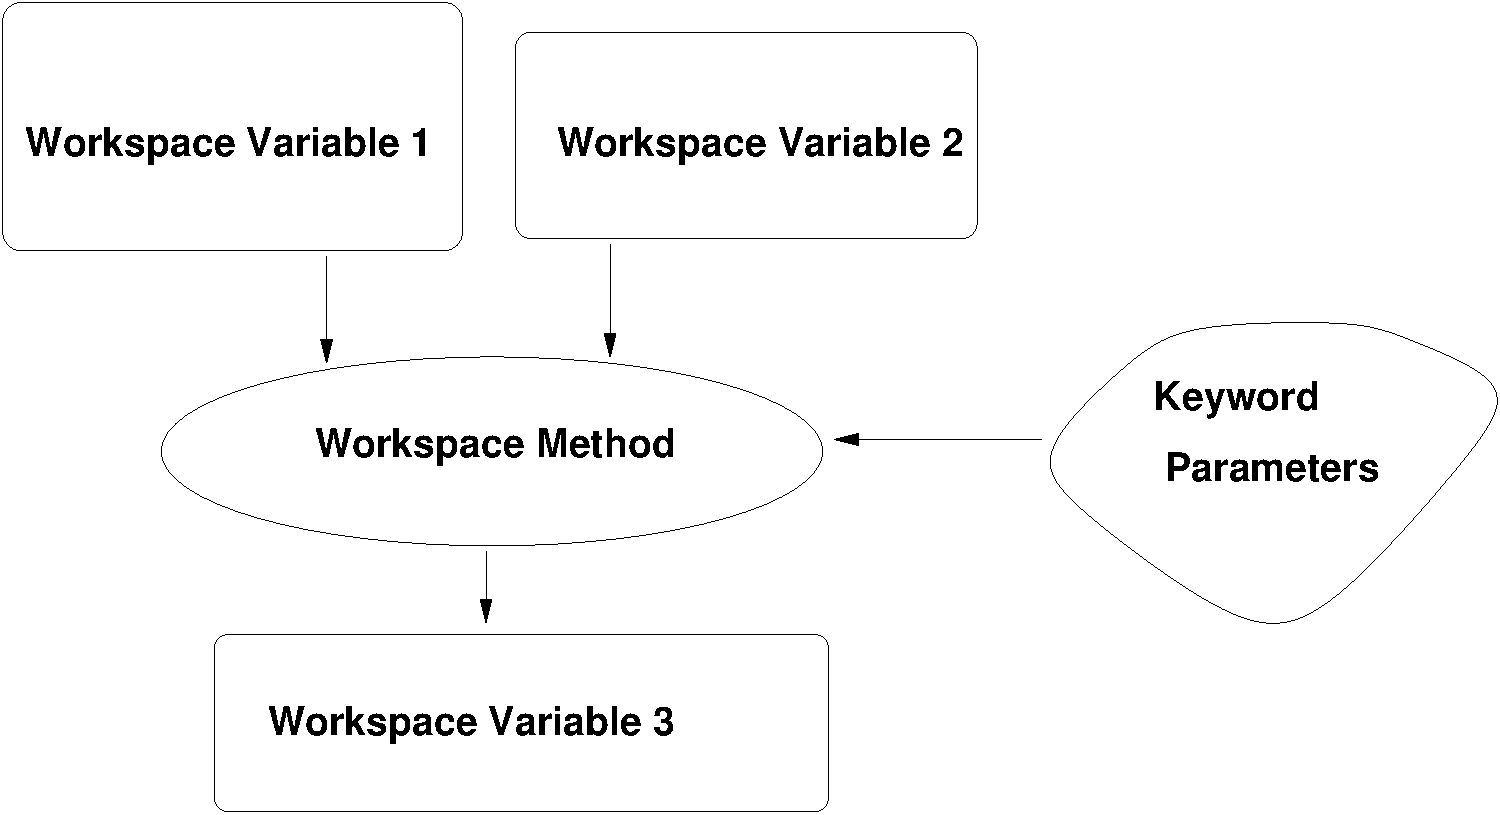
\includegraphics[width=\hsize,draft=false]{method}
    \caption{\emph{Specific}
        workspace methods act on specific workspace variables to
        generate other specific workspace variables. Additional input
        parameters can be specified as keyword parameters in the
        controlfile.}
    \label{fig:method}
  \end{center}
\end{figure}

It is important to note that the controlfile has a fixed and
well-defined syntax. This syntax is understood by the ARTS parser.
The great advantage of this concept is that it is very easy to add
new workspace variables and new workspace methods. The program has
an internal lookup table which lists all workspace methods, as well
as their input variables, output variables, and keyword
parameters. To add a new method, one just has to add an entry to
this lookup table, and write the code for the method itself. No
further changes to the program are necessary. In particular, no
changes to the program logic or to the parser. How such an extension
can be made practically is described in Section \ref{sec:development}.


\levelb{Generic Workspace Methods}
%=================================
\label{sec:concept:generic}

Generic methods (Figure \ref{fig:generic_method}) allow the user of the
program even more freedom than specific methods. A generic method is
for example \verb|VectorReadAscii|, which can be used to read any
workspace variable which is a vector from an ASCII file. For example
\begin{quote}
  \verb|VectorReadAscii(f_mono){"freqeuency_grid.aa"}|
\end{quote}
will read the specified file and generate the workspace variable
\verb|f_grid|.

\begin{figure}
  \begin{center}
    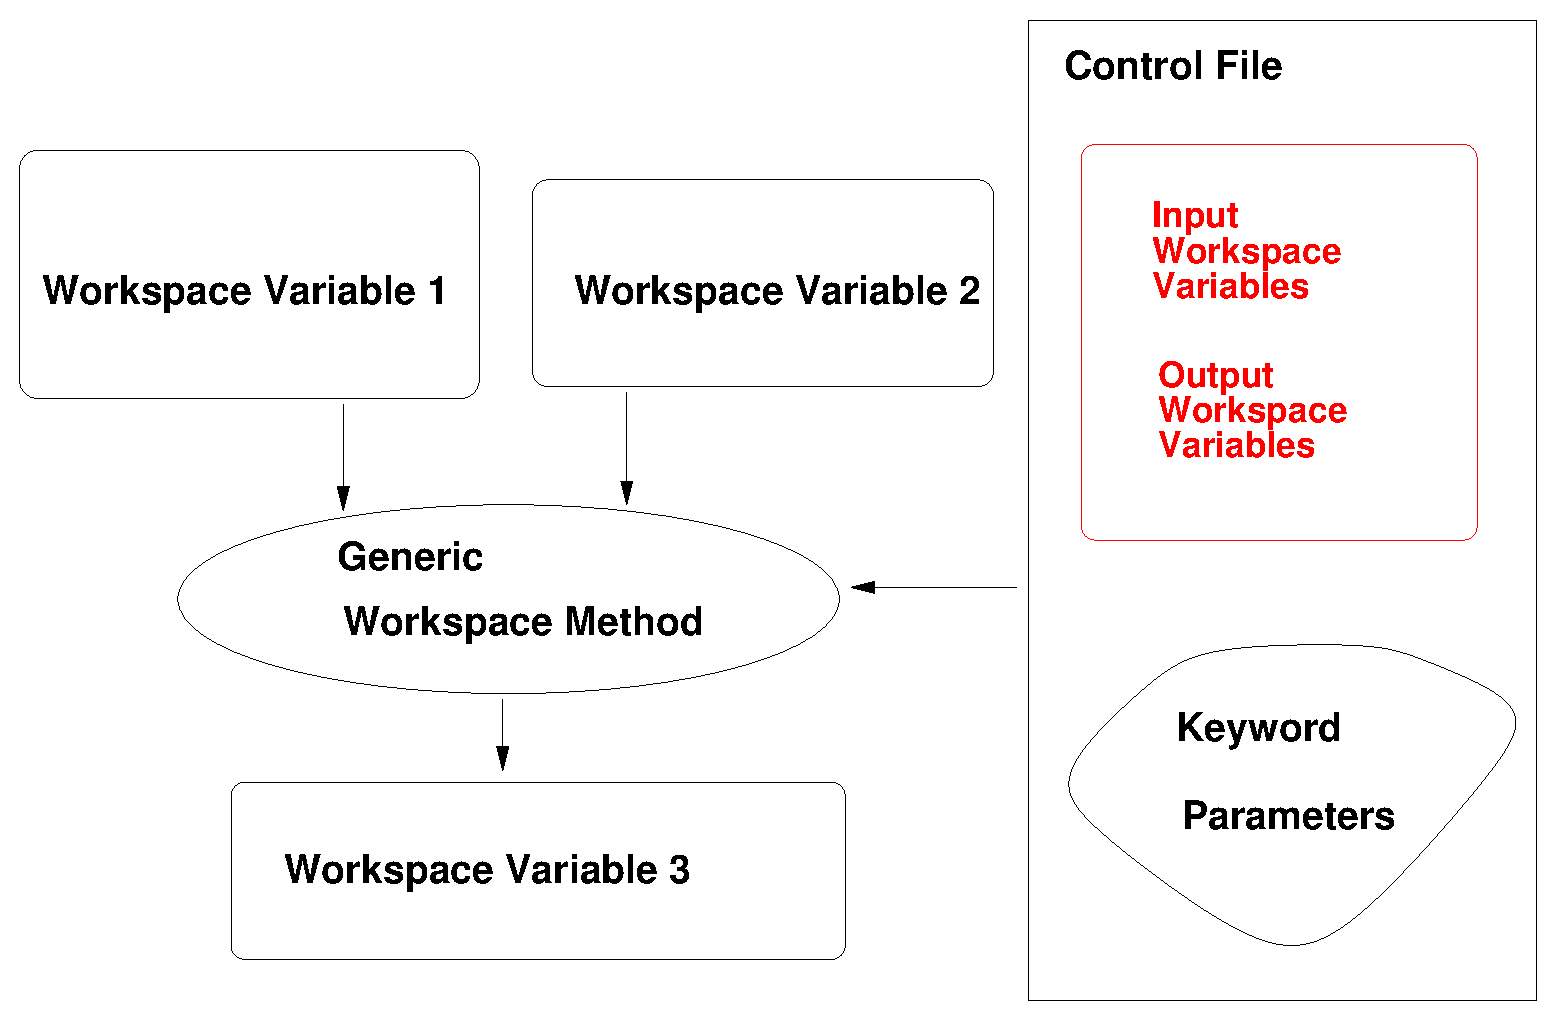
\includegraphics[width=\hsize,draft=false]{generic_method}
    \caption{For \emph{generic}
      workspace methods the workspace variables to act on are
        specified in the controlfile.}
    \label{fig:generic_method}
  \end{center}
\end{figure}

Generic methods are particularly useful for IO operations like in the
example above. No new IO functions are necessary for new workspace
variables, as long as they are of standard types already known to the
program (for example vectors or matrices). 

\levelb{Practical hints}
%=================================
\label{sec:concept:practical}

The subdirectory \verb|examples| of the \verb|doc| directory contains
some example controlfiles. You should study them to learn more about
how the program works. You can also run these controlfiles like this:
\begin{quote}
\begin{verbatim}
  arts absorption_example.arts
\end{verbatim}
\end{quote}
This assumes that you are inside the directory where the controlfiles
are, and that the \verb|arts| executable is in your path.  You can
also run all of the examples, by saying
\begin{quote}
\begin{verbatim}
  make check
\end{verbatim}
\end{quote}

ARTS offers a number of useful command line parameters. In general,
there is a short form and a long form for each parameter. The short
form consists of a minus sign and a single letter, whereas the long
form consists of two minus signs and a descriptive name. To get a full
list, type
\begin{quote}
\begin{verbatim}
  arts -h
\end{verbatim}
\end{quote}
or
\begin{quote}
\begin{verbatim}
  arts --help
\end{verbatim}
\end{quote}
Most useful at the beginning should be the \verb|-d|
(\verb|--describe|), \verb|-m| (\verb|--methods|), \verb|-w|
(\verb|--workspacevariables|), and \verb|-i| (\verb|--input|) flags.
For instance, the \verb|-d| (\verb|--describe|) flag gives you online
documentation for any workspace method or workspace variable. Usage:
\begin{quote}
\begin{verbatim}
  arts -d f_mono
\end{verbatim}
\end{quote}
will print documentation about the workspace variable \verb|f_mono|, which
happens to be the monochromatic frequency grid.

But what methods and variables are available? You can find out by
typing
\begin{quote}
\begin{verbatim}
  arts -m all
\end{verbatim}
\end{quote}
which will list all workspace methods, or by typing 
\begin{quote}
\begin{verbatim}
  arts -w all
\end{verbatim}
\end{quote}
which will list all workspace variables. As you can see, these lists
are quite long. But you can get more specific information:
\begin{quote}
\begin{verbatim}
  arts -m f_mono
\end{verbatim}
\end{quote}
will give you a list of all methods that can generate the workspace
variable \verb|f_mono|. Specific and generic methods are listed
separately. Generic methods are in this case all methods producing a
Vector, since \verb|f_mono| belongs to this group. A similar task is
performed by the \verb|-i| (\verb|--input|) flag, with the difference
that \verb|arts -i f_mono| will list those methods that require
\verb|f_mono| as \emph{input}, whereas \verb|arts -m f_mono| lists
those that produce \verb|f_mono| as output. Finally,
\begin{quote}
\begin{verbatim}
  arts -w absCalc
\end{verbatim}
\end{quote}
will give you all variables required by the method \verb|absCalc|
(the variable \verb|f_mono| happens to be one of them).

Using these command line parameters, it is easy to build up a
controlfile. The trick is, to start at the end. Say you want to
compute absorption coefficients. First of all, you have to find out
in which workspace variable these are stored. Look at the list
produced by \verb|arts -w all|. You can use \verb|arts -d| to look at
some candidates a bit more closely. This way, you will find out that
\verb|abs| is the variable you are looking for.

In the next step, you can use \verb|arts -m abs| to find all methods
that can calculate \verb|abs|. So, you will find the method
\verb|absCalc|. Now you can use \verb|arts -w absCalc| to find out the
required input variables of that method. Then you can use the
\verb|-m| flag again, to find the methods producing these variables,
and so on.

%%% Local Variables: 
%%% mode: latex
%%% TeX-master: "uguide"
%%% End: 

\include{in_and_out}
\include{atmosphere}
\include{rte_basics}
\include{complete_calcs}


\part{Atmospheric properties}
%-----
 %
% To start the document, use
%  \levela{...}
% For lover level, sections use
%  \levelb{...}
%  \levelc{...}
%
\levela{Gas Absorption}
 \label{sec:absorption}


%
% Document history, format:
%  \starthistory
%    date1 & text .... \\
%    date2 & text .... \\
%    ....
%  \stophistory
%
\starthistory
  2001-07-05 & Template created by Stefan Buehler.\\
  2001-10-05 & Line absorption part written, Nikolay Koulev\\
  2001-11-21 & Continuum absorption part written, Thomas Kuhn.\\
\stophistory
%
% Symbol table, format:
%  \startsymbols
%    ... & \verb|...| & text ... \\
%    ... & \verb|...| & text ... \\
%    ....
%  \stopsymbols
%
%
%\startsymbols
%  -- & -- & -- \\
% \label{symtable:wfuns}     
%\stopsymbols

% ============================================================================

% ============================================================================
% TKS definitions for the sections "Continuum Absorption" and 
% "Complete Absorption Models"
%
\def\deni{\rho_{\mbox{\rm i}}}
\def\denl{\rho_{\mbox{\rm l}}}
\def\denli{\rho_{\mbox{\rm l,i}}}
%
\def\imn{{N''}}
\def\ime{\epsilon^{''}_r}
\def\ree{\epsilon^{'}_r}
\def\er{\epsilon_r}
%
\def\bek{\rm b_{\rm 1,k}}
\def\bzk{\rm b_{\rm 2,k}}
\def\bdk{\rm b_{\rm 3,k}}
\def\bvk{\rm b_{\rm 4,k}}
\def\bfk{\rm b_{\rm 5,k}}
\def\bsk{\rm b_{\rm 6,k}}
%
\def\bekp{\rm \widehat{b}_{\rm 1,k}}
\def\bzkp{\rm \widehat{b}_{\rm 2,k}}
\def\bdkp{\rm \widehat{b}_{\rm 3,k}}
\def\bvkp{\rm \widehat{b}_{\rm 4,k}}
\def\bfkp{\rm \widehat{b}_{\rm 5,k}}
\def\bskp{\rm \widehat{b}_{\rm 6,k}}
%
\def\beks{\rm b^*_{\rm 1}}
\def\bzks{\rm b^*_{\rm 2}}
\def\bdks{\rm b^*_{\rm 3}}
\def\bvks{\rm b^*_{\rm 4}}
\def\bfks{\rm b^*_{\rm 5}}
\def\bsks{\rm b^*_{\rm 6}}
%
\def\bekps{\rm \widehat{b^*}_{\rm 1,k}}
\def\bzkps{\rm \widehat{b^*}_{\rm 2,k}}
\def\bdkps{\rm \widehat{b^*}_{\rm 3,k}}
\def\bvkps{\rm \widehat{b^*}_{\rm 4,k}}
\def\bfkps{\rm \widehat{b^*}_{\rm 5,k}}
\def\bskps{\rm \widehat{b^*}_{\rm 6,k}}
%
\def\air{\mbox{air}}
\def\am{\mbox{NH}_3}
\def\hzo{\mbox{H}_2\mbox{O}}
\def\nzo{\mbox{N}_2\mbox{O}}
\def\nz{\mbox{N}_2}
\def\oz{\mbox{O}_2}
\def\co{\mbox{CO}}
\def\coz{\mbox{CO}_2}
\def\clo{\mbox{ClO}}
%
\def\vmroz{VMR_{\mbox{\rm \small O}_{2}}}
%
\def\ptot{P_{\mbox{\rm \small tot}}}
\def\phzo{P_{\mbox{\rm \small H2O}}}
\def\pnz{P_{\mbox{\rm \small N2}}}
\def\poz{P_{\mbox{\rm \small O2}}}
\def\pda{P_{\mbox{\rm \small d}}}
\def\pdair{P_{\mbox{\rm \small air}}}
\def\pan{P_{\mbox{\rm \small air,N2}}}
\def\pcoz{P_{\mbox{\rm \small CO2}}}
%
\def\alphatot{\alpha_{\mbox{\rm \small tot}}} 
\def\alphal{\alpha_{\ell}} 
\def\alphac{\alpha_{\mbox{\small c}}}
\def\alphacs{\alpha_{\mbox{\rm \small c,s}}} 
\def\alphacf{\alpha_{\mbox{\rm \small c,f}}}
%
\def\alphampmotot{\alpha^{\mbox{\rm \small MPM87}}_{\mbox{\small tot}}} 
\def\alphampmmtot{\alpha^{\mbox{\rm \small MPM89}}_{\mbox{\small tot}}} 
\def\alphampmntot{\alpha^{\mbox{\rm \small MPM93}}_{\mbox{\small tot}}} 
\def\alphapwrtot{\alpha^{\mbox{\rm \small R98}}_{\mbox{\small tot}}} 
\def\alphacptot{\alpha^{\mbox{\rm \small CP98}}_{\mbox{\small tot}}} 
%
\def\alphampmol{\alpha^{\mbox{\rm \small MPM87}}_{\mbox{\small $\ell$}}} 
\def\alphampmml{\alpha^{\mbox{\rm \small MPM89}}_{\mbox{\small $\ell$}}} 
\def\alphampmnl{\alpha^{\mbox{\rm \small MPM93}}_{\mbox{\small $\ell$}}} 
\def\alphampml{\alpha^{\mbox{\rm \small MPM}}_{\mbox{\small $\ell$}}} 
\def\alphapwrl{\alpha^{\mbox{\rm \small R98}}_{\mbox{\small $\ell$}}} 
\def\alphacpl{\alpha^{\mbox{\rm \small CP98}}_{\mbox{\small $\ell$}}} 
%
\def\alphampmoc{\alpha^{\mbox{\rm \small MPM87}}_{\rm c}} 
\def\alphampmmc{\alpha^{\mbox{\rm \small MPM89}}_{\rm c}} 
\def\alphampmnc{\alpha^{\mbox{\rm \small MPM93}}_{\rm c}} 
\def\alphapwrc{\alpha^{\mbox{\rm \small R98}}_{\rm c}} 
\def\alphacpc{\alpha^{\mbox{\rm \small CP98}}_{\rm c}} 
%
\def\gamk{\gamma_{\mbox{\rm \small k}}}
\def\gamc{\gamma_{\mbox{\rm \small c}}}
%
\def\ws{w_{\mbox{\rm \small s,k}}}
\def\xs{x_{\mbox{\rm \small s,k}}}
\def\wf{w_{\mbox{\rm \small f,k}}}
\def\xf{x_{\mbox{\rm \small f,k}}}
%
\def\wn{\bar{\nu}}
\def\nucc{\nu_{\mbox{\rm \small c}}}
\def\nucut{\nu_{\mbox{\rm \small cutoff}}}
\def\nuo{\nu_{\mbox{\rm \small 0}}}
\def\nuk{\nu_{\mbox{\rm \small k}}}
%
\def\shape{F(\nu,\nuk)}
\def\shapec{F_{c}(\nu,\nuk)}
\def\shapefp{f_{c}(\nu,+\nuk)}
\def\shapefm{f_{c}(\nu,-\nuk)}
\def\shapefpm{f_{c}(\nu,\pm\nuk)}
\def\inten{S_{\mbox{\rm \small k}}(T)}
\def\inteno{S_{\mbox{\rm \small k}}(300\,K)}
\def\intencp{S_{\mbox{\rm \small 0}}(T)}
%
\def\cx{C_{\mbox{\rm \small x}}}
\def\cs{C_{\mbox{\rm \small H}_{2}\mbox{\rm \small O}}} 
\def\cf{C_{\mbox{\rm N}_{2}}} 
\def\cxo{C^{\mbox{\rm o}}_{\mbox{\rm \small X}}} 
\def\cso{C^{\mbox{\rm o}}_{\mbox{\rm \small H}_{2}\mbox{\rm \small O}}} 
\def\cfo{C^{\mbox{\rm o}}_{\mbox{\rm \small N}_{2}}} 
\def\cao{C^{\mbox{\rm o}}_{\mbox{\rm \small air}}}
\def\cdo{C^{\mbox{\rm o}}_{\mbox{\rm \small d}}}
\def\xx{{\rm n}_{\mbox{\rm \small  x}}} 
\def\xs{{\rm n}_{\mbox{\rm \small  s}}} 
\def\xf{{\rm n}_{\mbox{\rm \small  f}}} 
\def\xd{{\rm n}_{\mbox{\rm \small  d}}}
%
% ============================================================================


                                          

In general there are three types of absorption/emission spectra:
\begin{itemize}
\item sharp lines of finite width
\item aggregations (series) of lines called bands
\item continua extending over a broad range of wavelengths, with
      no single lines in it.
\end{itemize}
This section is therefore firstly devised to give a short theoretical
overview of the absorption quantities which are used in ARTS. The
presentation of the calculation methods within ARTS of these
quantities is the second goal. There are two major subsections which
deal separately with the respective types of spectra regarded by ARTS,
lines and continua.  The second one extends beyond the scope of mere
treatment of the continua and thus gives an integrated view of
continua and spectral lines.

% ================================================================================
% The following section is written by Nikolay Koulev, iup Bremen, nkoulev@uni-bremen.de
% ================================================================================

\levelb{Line Absorption}
%-----------------------
\label{sec:line_absorption}

 
We will introduce here the main concepts concerning
line absorption. The approach, however, does not aim  at the
derivation, but rather at the presentation the following expressions.

Any line is presented by the corresponding profile of the absorption/emission
coefficient as a function of the frequency, in our case that of the
absorption - given by the quantity $\alpha(\nu)$. The latter dependency
is related to other quantities, which express the three
characteristics of a single line uniquely describing it - position,
strength and shape. 
The strength, or better the line intensity, is given by the quantity
$S(T)$, where $T$ is absolute temperature. The shape and the position are expressed through the
line-shape function $F(\nu)$. Thus we have the relation    
\begin{equation}\label{abs_coeff}
  \alpha(\nu)=nS(T)F(\nu)
\end{equation} 
where $n$ is the number density of the absorber, \citet{goodyandyung:89}. The line-shape
function is normalized as follows

\begin{equation}\label{line_shape_norm}
  \int F(\nu)d\nu=1
\end{equation}
The values of $S(T)$ at reference temperature $T_0$ are contained in
spectroscopic databases. The conversion to different temperatures is
done by
\begin{equation}\label{line_intensity}
  S(T)=S(T_0)~\frac{Q(T_0)}{Q(T)}~\frac{e^{-E_f/(kT)}
    - e^{-E_i/(kT)}}{e^{-E_f/(kT_0)} - e^{-E_i/(kT_0)}}
\end{equation}
given the energies $E_f$ and $E_i$ of the two levels between which the
transition occurs as well as the partition function~~$Q(T)$, \citet{rothman:98}. The
databases contain the lower state energy $E_l$ tabulated along with
the $S$ and the transition frequency $\nu$, so that the upper state
energy can be computed by $E_u$=$E_l$+h$\nu$. Partition functions for
all molecular species are also available along with spectroscopic
databases, either in the form of tabulated values for a set
temperatures, or in the form of FORTRAN routines. One can obtain the
total absorption coefficient by adding the absorption of all spectral
lines of all molecular species.

The problem of determining the explicit kind of the line-shape
functions is treated in the following subsection. Another one is
dedicated to the partition functions and their calculation..


\levelc{Line Shape Functions} Up to date there is no way to calculate
the line-shape functions analytically just from the theoretical
expressions of quantum dynamics, statistical physics, and theoretical
mechanics. Certain approximations have to be made to account for
different physical phenomena related to the absorption/emission
process or to suit better the calculation of different parts of the
spectral line.

There are three phenomena which contribute to the line-shape. These
are, in increasing order of importance, the finite lifetime of an
excited state in an isolated molecule, the thermal movement of the gas
molecules, and their collisions with each other. They result in
corresponding effects to the line-shape: natural broadening, Doppler,
and pressure broadening. Of these, the first one is completely
negligible compared to the other two. Nevertheless, we will pay a
special attention to the natural broadening because its implications
are of a conceptual importance for the broadening processes.

The spectral line shape can be derived in the case of natural
broadening from basic physical considerations and a well-known Fourier
transform theorem from the time to the frequency domain, \citet{thorne:99}. If we
consider classically the spontaneous decay of the excited state of
two-level system in the absence of external radiation, then population
$n$ of these level decreases according to
\begin{equation}\label{spon_decay_diff}
  \frac{dn(t)}{dt} = -A\,n(t)
\end{equation}
where $A$ is Einstein A coefficient, which equation can also be
interpreted as the rate of the spontaneously emitted photons because
of decay. This relation is more usefully in this case to be written in
the following manner 
\begin{equation}\label{spon_decay_exp}
  n(t)=n(0)~e^{-At}=n(0)e^{-t/\tau}
\end{equation}
where $ \tau$ is the mean lifetime of the excited state. Thus the
number of spontaneously emitted photons and in this way the flux of
the emitted radiation then will be proportional to $n$. Therefore we
can write for the flux $L$ that
\begin{equation}\label{flux}
  L(t)=L(0)~e^{-t/ \tau}=L(0)~e^{-\gamma t}
\end{equation}
By the afore mentioned theorem, multiplying in the time domain by
$e^{-\gamma t}$ is equivalent to convolving in the frequency domain
with a function $1/[\nu^2 - (\gamma/4\pi)^2]$. Accordingly the line
profile of a spectral line at frequency $ \nu_0$ as a normalized
line-shape function will be, as difined in \citet{thorne:99},
\begin{equation}\label{natural_lorentz}
  F(\nu)=\frac{1}{\pi}\frac{\gamma/4\pi}{(\nu - \nu_0)^2 + (\gamma/4\pi)^2}
\end{equation}
This gives a bell-shaped profile and the function itself is called
Lorentzian. The dependence on the position of the line is apparent
through $\nu_0$, that is why some authors prefer to denote the
function by $F(\nu,\nu_0)$.  The result is important because of two
major reasons.  Firstly, without the natural broadening the line would
be the delta function~$\delta (\nu - \nu_o)$, as pointed out in
\citet{bernath:95}. So the spontaneous decay of the excited state is
responsible for the finite width and the certain shape of the
line-shape function. Secondly, the Lorentzian type of function comes
significantly into play when explaining some of the other broadening
effects or the complete picture of the broadened line, \citet{thorne:99}.

The second effect, Doppler broadening, is important for the upper
stratosphere and mesosphere for microwave frequencies. The line-shape
follows the velocity distribution of the particles. Under the conditions
of thermodynamic equilibrium, we have  a probability distribution for
the relative velocity $u$ between the gas molecule and the observer 
of Maxwell type 
\begin{equation}\label{maxwell_distribution}
  p(u)=\sqrt{\frac{m}{2\pi kT}}~~exp~\left[-\frac{mu^2}{2kT}\right]
\end{equation}
where $m$ is the mass of the molecule. Using then the formula for the
Doppler shift for the non-relativistic region~~  $\nu$- $\nu_0$ =
$\nu_0$$u$ / $c$ , one can easily derive the line-shape function, \citet{bernath:95}, 
\begin{equation}
 F_D(\nu)=\frac{1}{\gamma_D\sqrt{\pi}}~~exp~\left[-\left(\frac{\nu - \nu_0}{\gamma_D}\right)^2\right]
\end{equation}
where the quantity $\gamma_D$ is called Doppler line width and equals
\begin{equation}
 \gamma_D=\frac{\nu}{c}\sqrt{\frac{2kT}{m}}
\end{equation}
In contrast to the afore mentioned line-shape function for the natural
broadening the Doppler broadening is expressed by a Gaussian
line-shape function $F(\nu)$. The Doppler line width $\gamma_D$ is so
defined that it is equal to the half width at half of the maximum
(HWWM) of the line-shape function. The same way of notating is used
for all other width parameters $\gamma_{xy}$ below.

It can be said without any exaggeration that the pressure broadening
effect is the most complicated one among the others and still
represents a complex theoretical task to be tackled, and is in the
same time of major experimental importance. So far, there is no way to
calculate analytically from the basics the profile of a pressure, or
collisional, line through a single approach near the line center as
well as in the far wing region. The various approximations, which are
therefore used, are immanently limited to the certain line regions
they deal with.  The most popular among these approximations is the
{\it{impact~approximation}} which postulates that the duration of the
collisions of the gas particles is very small compared to the average
time between the collisions. Lorentz was the first to achieve a result
exploiting this approach, the Lorentz line-shape function:
\begin{equation}\label{pressure_lorentz}
 F_L(\nu)=\frac{\gamma_L}{\pi}\frac{1}{(\nu-\nu_0)^2+\gamma_L^2}
\end{equation}
where $\gamma_L$ is the Lorentz line width, \citet{thorne:99}. As one
can see, the result Eq.\,\ref{pressure_lorentz} is pretty similar to
Eq.\,\ref{natural_lorentz} but the specific line parameters $\gamma$
and $\gamma_L$ make them differ significantly in the corresponding
frequency regions of interest. For atmospheric pressures $\gamma_L$ is
much greater and because of that, of experimental
significance in contrast to $\gamma$.\\
Elaborating the model of Lorentz, van Vleck and Weisskopf made a
correction to it, \citet{vanvleck:45},particularly for the microwave
region:
\begin{equation}\label{eq:vvw}
 F_{VVW} (\nu)=\left(\frac{\nu}{\nu_0}\right)^2\frac{\gamma_L}{\pi}
 \left[\frac{1}{(\nu-\nu_0)^2+\gamma_L^2}+\frac{1}{(\nu+\nu_0)^2+\gamma_L^2}\right]
\end{equation}
which can be reduced to a Lorentzian for $(\nu-\nu_0) << \nu_0$ and $0
<< \nu_0$. Except for the additional factor $(\nu/\nu_0)^2$ ,
$F_{VVW}$ can be regarded as the sum of two $F_L$, or respectively
lines, one with its center frequency at $\nu_0$, the other at
$-\nu_o$.

The van Vleck and Huber lineshape \citep{vanvleckhuber:77} is similar
to Eq.\,\ref{eq:vvw}, except for the factor $(\nu/\nu_0)^2$ which is
replaced by $(\nu * \tanh(h*\nu/(2kT)))/(\nu_0 *
\tanh(h*\nu_0/(2kT)))$, with $k$ the Boltzmann constant, $h$ the Planck
constant, and $T$ the atmospheric temperature (the denominator is
actually a consequence of the line strength definition in the
spectroscopic catalogs). The lineshape Eq.\,\ref{eq:vvw} with this
factor can be used for the entire frequency range, since
the microwave approximation: $\tanh(x) = x$, that leads to the factor
$(\nu/\nu_0)^2$, is not made.

The combined picture of a simultaneously Doppler and pressure
broadened line is the next step of the approximations development. The
line-shape function has to approximated in this case by the Voigt line-shape
function 
\begin{equation}\label{voigt}
 F_{Voigt}(\nu,\nu_0)= \int F_L(\nu,\nu')~F_D(\nu',\nu_0)~d\nu'
\end{equation}
though there's no strict justification for its use - the two processes
are assumed to act independently, which in reality is not the
fact. Regardless of this flaw, it is the only way up to date to model
the combination of the broadening processes. The integral in Eq.\,\ref{voigt}
can not be computed analytically, so certain approximation algorithms
must be used.


Another possibility would be the combination of the last two equations
Eq.\,\ref{eq:vvw} and Eq.\,\ref{voigt}. The respective result then will be 
\begin{equation}\label{voigt_mirror}
 F_S=\left(\frac{\nu}{\nu_0}\right)^2~[F_{Voigt}(\nu,\nu_0)+F_{Voigt}(\nu,-\nu_0)]
\end{equation}
The advantage of such a model is that it behaves like a van
Vleck-Weisskopf line-shape function in the high pressure limit and
like a Voigt one in the low pressure limit. There is one important
caveat to the equation Eq.\,\ref{voigt_mirror}: it has to be made sure that the
algorithm that is used to compute the Voigt function really produces a
Lorentz line in the high pressure limit. Another point of significance
is the demand that the model yields meaningful results far from the
line center, since the line center from the ``mirror'' line at
-$\nu_0$ is situated approximately 2$\nu_0$ away from the frequency
$\nu_0$ of computation. The algorithm of \citet{Drayson:76} and
\citet{Oliveiro:77} was explicitly checked to satisfy both
requirements, while this was found to be not true for some other
algorithms, commonly used for Voigt-shape computation. In particular,
the it is not true for the Hui-Armstrong-Wray Formula, as defined in
\citet{hui:78} and in Equation 2.60 of \citet{pwr:93}. So, provided
the stated above is fulfilled, the $F_S$ line shape gives a smooth
transition from high tropospheric pressures to low stratospheric ones,
and should be valid near the line centers throughout the microwave region.






\levelc{Partition Functions}

The treatment of the partition functions is directly related to the molecular
energy states and their statistical distribution during the
radiation process. 

In any case of spectroscopic interest the free molecules of a gas are
not optically thick at all frequencies, so the radiation energy is not
represented by blackbody radiation. The most common assumption made,
which is sufficient in the case of tropospheric and low stratospheric
research, is the {\textit{local thermodynamic equilibrium}\nocorr} or
{\textit{LTE }\nocorr}. According to it, it's possible to find a common temperature,
which may vary from place to place, that fits the Boltzmann energy
population distribution and the Maxwell velocities distribution.
This practically means, that under $LTE$ the collisional processes
must be of greater importance than radiative ones. In other words,
an excited state must have a higher probability of de-excitation by
collision than by spontaneous radiation. This is the important
factor which makes natural broadening differ quantitatively so much
from the pressure (collisional) one, though both are described
qualitatively almost identically by Lorentzian line- shape
functions.

According to the Maxwell-Boltzmann distribution law, in $LTE$ the total number
of gas particles $N_n$  in a state $E_n$ is given by 
\begin{equation}\label{maxwell_distribution}
 N_n=N_0\frac{g_n}{g_0}e^{-E_n/kT}
\end{equation}
where $N_0$ is particle number in the ground state, and $g_n$, $g_o$
are the statistical weights (degeneracies) of the $n-$state and the
ground state, \citet{gordyandcook:70}. Thus the total particle number $N$ is given by
\begin{equation}\label{total_part_number}
 N=\frac{N_0}{g_0}\sum_{n=0}^\infty g_n~e^{-E_n/kT}=\frac{N_0}{g_0}~Q(T)
\end{equation}
The quantity $Q(T)$ is the {\it{partition function}\nocorr} of the
gas, which generally speaking describes the energy states distribution
of the gas particles. 

The partition function for a perfect gas molecule can be represented
by the product of the {\it{translational}\nocorr} and the
{\it{internal}\nocorr} partition functions, as defined in \citet{herzberg:45},
\begin{equation}\label{partition_f_general}
 Q  =  Q_{tr}~Q_{int}
\end{equation}
bearing in mind that the respective energies, translational and
internal, are independent of each other. The first quantity $Q_{tr}$ accounts
for the distribution of the translational energy of the gas particles
- it takes into account that the translational velocities of the
particles fulfill the Maxwell distribution. The quantity, however,
which we are interested in in (3.3) is the {\it{internal}\nocorr}
partition function (or the {\it{total internal partition  function}\nocorr}
 because the transitions between the discrete
internal energy states are responsible for the absorption or emittance
of radiation. Accordingly $Q_{int}$ describes the
distribution of energy among the internal energy states of the gas
particles.

The internal partition function for free gaseous molecules is a
function of the electronic, the vibrational, the rotational, and the
nuclear spin states. An approximation is used in
\citet{gordyandcook:70} in order to display the individual
contribution explicitly
\begin{equation}\label{int_partition}
 Q_{int}=Q_e~Q_v~Q_r~Q_n
\end{equation}
and thus the interaction between these various states is neglected.
For practically all polyatomic molecules the excited electronic states
are entirely negligible to those of the ground states, i.e. $Q_e=1$ .
Only for the very few polyatomic molecules with a multiplet ground
state ($NO_2$ , $ClO_2$ , and free radicals) has the
electronic contribution to be considered.\\
If we neglect the anharmonicities, the vibrational partition function,
with vibrational energy levels measured with respect to the ground
state for the {\it harmonic oscillator}, is acording \citet{herzberg:45}
\begin{equation}\label{vib_partition}
 Q_v=\left(\sum_{\nu_1}e^{-\nu_1 h\omega_1/kT}\right)\left(\sum_{\nu_2}e^{-\nu_2 h\omega_2/kT}\right)...
\end{equation}
where $\nu_1$, $\nu_2$,..., the vibrational quantum numbers, can each
have the values 0,1,2,... and $\omega_1$, $\omega_2$,..are the
frequencies of the fundamental modes of vibration. The summation is
taken over all values of $\nu_1$, $\nu_2$,..., and each fundamental
mode is counted separately. This result is valid for non-degenerate
vibrations. If we use the simple expression for geometric progression
\begin{equation}\label{geom_progression}
 \sum_{\nu_i}e^{-\nu_i h\omega_i/kT}=\frac{1}{1-e^{h\omega_i/kT}}
\end{equation}
and the degeneracies $d_1$, $d_2$,... of the fundamental modes, we get
finally for the vibrational partition function
\begin{equation}\label{vib_partition_fin}
Q_v=\left(1-e^{h\omega_1/kT}\right)^{-d_1}\left(1-e^{h\omega_2/kT}\right)^{-d_2}...
\end{equation}

The rotational partition function looks differently for the different
symmetry types of molecules.
For diatomic and linear  polyatomic molecules with no center of
symmetry the corresponding expression is, as defined in \citet{gordyandcook:70}
\begin{eqnarray}\label{rot_partition}
Q_r & = & \sum_{J=0}^\infty (2J+1)e^{-hBJ(J+1)/kT}\nonumber\\
   & = & \frac{kT}{hB}+\frac{1}{3}+\frac{1}{15}\frac{hB}{kT}+\frac{4}{315}\left(\frac{hB}{kT}\right)^2+...\nonumber\\
   & \cong & \frac{kT}{hB}
\end{eqnarray}
For {\it{ rigid symmetric-}}, {\it{asymmetric-}}, and {\it{spherical}} top molecules there are also
other factors to be taken into consideration, such as the
spatial structure of the molecules, nuclear spin, inversion and
internal rotation. The general expression in the case of a 
{\it{ rigid symmetric-}} top molecule according \citet{herzberg:45}
is
\begin{equation}\label{rot_partition_symtop}
Q_r  =  \frac{1}{\sigma}\sum_{J=0}^\infty \sum_{K=-J}^{J}(2J+1)~e^{-h[BJ(J+1)+(A-B)K^2]/kT}
\end{equation}
where $\sigma$ is measure of the degree of symmetry. The usual
symmetric top has $C_3$ or $C_{3\nu}$ symmetry, therefore $\sigma$ = 3. To a good
approximation, the summation above can expressed as in \citet{gordyandcook:70}
\begin{equation}\label{rot_partition_top_appro}
Q_r  = 
\frac{1}{\sigma}\left[\left(\frac{\pi}{B^2A}\right)\left(\frac{kT}{h}\right)^3\right]^{1/2}=
\frac{5.34\times 10^6}{\sigma}\left(\frac{T^3}{B^{2}A}\right)^{1/2}
\end{equation}
For an  {\it{asymmetric}} top the formula would then be 
\begin{equation}\label{rot_partition_asymtop}
Q_r = \frac{5.34\times 10^6}{\sigma}\left(\frac{T^3}{ABC}\right)^{1/2}
\end{equation}
and for a {\it{spherical}} top, using the current notation of
\citet{gordyandcook:70} in the respective expression in \citet{herzberg:45},
\begin{equation}\label{rot_partition_sphetop}
Q_r = \frac{5.34\times 10^6}{\sigma}\left(\frac{T^3}{A^3}\right)^{1/2}
\end{equation}








\levelc{Line Catalogs} There are several spectroscopic catalogs
implemented in ARTS: HITRAN, JPL, MYTRAN, and the ARTS inherent
catalog format.

Special attention will be paid here only to the inherent format in ARTS.
To keep track with the changes in the catalog format, every catalog file
must start with $ARTSCAT-x$ , where for current version $x=2$.  Files
with different or missing version will be rejected. The current
version is stored in the private member variable mversion. It can be
read with the member function Version, which returns a String `ARTSCAT-x'.
After the version tag (ARTSCAT-x), ARTS outputs the number of lines
when catalog files are written. This number is not used by reading
routines, though.

The line catalog should not have any fixed column widths because the
precision of the parameters should not be limited by the format. The
catalog can then be stored in principle as binary or ASCII, though
currently are implemented only ASCII files. In the ASCII version
the columns are separated by one or more blanks. The line format is
then specified by only the order and the units of the columns. As the
catalog entry for each transition can be quite long, it can be broken
across lines in the ASCII file. Each new transition is marked with an
`@' character.  The first column will contain the species and isotope,
following the naming scheme described below. Scientific notation is
allowed, e.g. 501.12345e9.  Note that starting with ARTSCAT-2, the
intensity is per molecule, i.e., it does not contain the isotopic
ratio. This is similar to JPL, but different to HITRAN.  The line
format is:

\begin{verbatim}

Col  Variable                     Label    Unit     
-----------------------------------------------      
 0   `@'                         ENTRY        -     
 1   name                         NAME        -     
 2   center frequency                F       Hz     
 3   pressure shift of F           PSF    Hz/Pa    
 4   line intensity                 I0   m^2/Hz     
 5   reference temp. for I0       T_I0        K
 6   lower state energy           ELOW        J    
 7   air broadened width          AGAM    Hz/Pa     
 8   self broadened width         SGAM    Hz/Pa
 9   AGAM temp. exponent          NAIR        -     
10   SGAM temp. exponent         NSELF        - 
11   ref. temp. for AGAM, SGAM   T_GAM        K
12   number of aux. parameters   N_AUX        -
13   auxiliary parameter          AUX1        -
14   ... 
15   error for F                    DF       Hz
16   error for I0                  DI0        %
17   error for AGAM              DAGAM        %
18   error for SGAM              DSGAM        %
19   error for NAIR              DNAIR        %
20   error for NSELF            DNSELF        %
21   error for PSF                DPSF        %
22   quantum number code         QCODE           
23   lower state quanta         QLOWER            
24   upper state quanta         QUPPER            
25   information source of F                      IF
26   information source of I0                     II0
27   information source of line width variables   ILW
28   information source of pressure shift         IPSF
29   information source of auxiliary parameters   IAUX
\end{verbatim}
The parameters 0-12 must be present, the others can be missing, since
they are not needed for the calculation. For the error fields (15-21),
a~$-1$ means that no value exists. Fields 22-29 are strings inside quotes
\verb ""  for maximum flexibility.\\
Thus a valid ARTS line file would be:
\begin{verbatim}
ARTSCAT-2 2
@ CH4-211 1011349857.063 0 2.96070344144819e-27 296
2183.6851 13314.2468393782 21302.7949430052 0.75 0.75 296 0
@ O3-666 1088246622.54 0 2.82913939200384e-22 296
522.5576 21361.9693734024 27723.2206411054 0.76 0.76 296 0
\end{verbatim}
Some species need special parameters that are not needed by other
species (for example overlap coefficients for $O_2$). In the case of
oxygen two parameters are sufficient to describe the overlap, but
other species, e.g., methane, may need more coefficients. The default
for \texttt{N\_AUX} is zero. In that case, no further \texttt{AUX}
fields are present.







\levelc{Species specific data}

The following part treats the species related data in ARTS - all
currently implemented species with the respective molecular masses,
isotopic ratios, partition functions, and the sources for this
information. 

Table \ref{table:impl_secies} lists the implemented species in ARTS.
The first row gives the ARTS molecule name, the second the ARTS
isotope name (these two identify the species within ARTS). The third
row gives the number of this species in the MYTRAN catalog, the fourth
the one used in HITRAN96, and the fifth the corresponding tag numbers
of the JPL00 catalog.



\begin{longtable}{lllll}
 K & K & K & K & K \kill
%
% --------------------- only begin of table ------------------------------

 \hline
 {\it ARTS }& {\it ARTS }& {\it MYTRAN}& {\it HITRAN}& {\it JPL00}\\
 {\it Name}& {\it Isotope}& {\it Tag}& {\it Tag}& {\it Tag}\\ 
 \hline
 \endfirsthead
% --------------------- every page begin of table ------------------------
 \hline
 {\it ARTS }& {\it ARTS }& {\it MYTRAN}& {\it HITRAN}& {\it JPL00}\\
 {\it Name}& {\it Isotope}& {\it Tag}& {\it Tag}& {\it Tag}\\ 
 \hline
 \endhead
% --------------------- every page end of table ------------------------
 K & K & K & K & K \kill
 \hline
 \caption[]{(continued)}\\
 \endfoot
% --------------------- only end of table ------------------------------
 K & K & K & K & K \kill
 \hline
 \caption{Implemented species in ARTS} 
 \label{table:impl_secies}
 \endlastfoot
% --------------------- body of table ---------------------------------- 

 

  H2O& 161&  11&    11&  18003, 18005\\
     & 181&  12&    12&  20003\\
     & 171&  13&    13&  19003\\
     & 162&  14&    14&  19002\\
     & 182&  -1&    15&  21001\\
     & 172&  -1&    16&       \\
     & 262&  -1&    -1&  20001\\
     &SelfContStandardType&             -1&  -1 & \\      
     &ForeignContStandardType&          -1&  -1 & \\  
     &ForeignContMaTippingType&         -1&  -1 & \\      
     &ContMPM93&                        -1&  -1 & \\      
     &SelfContCKD24&                    -1&  -1 & \\      
     &ForeignContCKD24&                 -1&  -1 & \\ 
     &ForeignContATM01&                 -1&  -1 & \\         
     &CP98&                             -1&  -1 & \\      
     &MPM87&                            -1&  -1 & \\      
     &MPM89&                            -1&  -1 & \\      
     &MPM93&                            -1&  -1 & \\      
     &PWR98&                            -1&  -1 & \\  


\hline                  
  CO2& 626&  21&    21&\\
     & 636&  22&    22&\\
     & 628&  23&    23&  46013\\
     & 627&  24&    24&  45012\\
     & 638&  25&    25&\\
     & 637&  26&    26&\\
     & 828&  27&    27&\\
     & 728&  28&    28&\\
     &SelfContPWR93&    -1&-1&\\
     &ForeignContPWR93& -1&-1&\\
\hline                  
  O3& 666&  31&    31&  48004, 48005,\\
    &    &    &      &  48006, 48007,\\
    &    &    &      &  48008\\
    & 668&  32&    32&  50004, 50006\\
    & 686&  33&    33&  50003, 50005\\
    & 667&  34&    34&  49002\\
    & 676&  35&    35&  49001\\
\hline                  
  N2O& 446&  41&    41&  44004, 44009,\\
     &    &    &      &  44012\\
     & 456&  42&    42&  45007\\
     & 546&  43&    43&  45008\\
     & 448&  44&    44&  46007\\
     & 447&  -1&    45&\\
\hline                   
  CO&   26&  51&    51&  28001\\
    & 36&  52&    52&  29001\\
    & 28&  53&    53&  30001\\
    & 27&  -1&    54&  29006\\
    & 38&  -1&    55&\\
    & 37&  -1&    56&\\
\hline                  
  CH4& 211&  -1&    61&\\
     & 311&  -1&    62&\\
     & 212&  -1&    63&  17003\\
\hline                  
  O2& 66&  71&    71&  32001, 32002\\
    & 68&  72&    72&  34001\\
    & 67&  73&    73&  33002\\
    &SelfContStandardType&   -1        &-1&     \\
    &SelfContMPM93&          -1        &-1&     \\
    &SelfContPWR93&          -1        &-1&     \\
    &PWR98&                  -1        &-1&     \\ 
    &PWR93&                  -1        &-1&     \\
    &PWR88&                  -1        &-1&     \\  
    &MPM93&                  -1        &-1&     \\
    &MPM92&                  -1        &-1&     \\
    &MPM89&                  -1        &-1&     \\
    &MPM85&                  -1        &-1&     \\
\hline                  
  NO& 46&  81&    81&  30008\\
    & 56&  -1&    82&\\
    & 48&  -1&    83&\\
\hline                  
  SO2& 626&  91&    91&  64002, 64005\\
     & 646&  92&    92&  66002\\
     & 636&  93&    -1&  65001\\
     & 628&  94&    -1&  66004\\
\hline                  
  NO2& 646&  101&   101&  46006\\
\hline                  
  NH3& 4111&  111&   111&  17002, 17004\\
     & 5111&  112&   112&  18002\\
     & 4112&  -1&    -1&  18004\\
\hline                  
  HNO3& 146&  121&   121&  63001, 63002,\\
      &    &     &      &  63003, 63004,\\
      &    &     &      &  63005, 63006\\
\hline                  
  OH& 61&  131&   131&  17001\\
    & 81&  132&   132&  19001\\
    & 62&  133&   133&  18001\\
\hline                  
  HF& 19&  141&   141&  20002\\
    & 29&  -1&    -1&  21002\\
\hline                  
  HCl&15&  151&   151&  36001\\
     &17&  152&   152&  38001\\
     &25&  -1&    -1&  37001\\
     &27&  -1&    -1&  39004\\
\hline                  
  HBr& 19&  161&   161&  80001\\
     & 11&  162&   162&  82001\\
\hline                  
  HI& 17&  -1&   171&\\
\hline                  
  ClO& 56&  181&   181&  51002, 51003\\
     & 76&  182&   182&  53002, 53006\\
\hline                  
  OCS& 622&  191&   191&  60001\\
     & 624&  192&   192&  62001\\
     & 632&  193&   193&  61001\\
     & 822&  194&   194&  62002\\
     & 623&  195&   195&       \\
\hline                  
  H2CO& 1126&  201&   201&  30004\\
      & 1136&  202&   202&  31002\\
      & 1128&  203&   203&  32004\\
      & 1226&  -1&    -1&  31003\\
      & 2226&  -1&    -1&  32006\\
\hline                  
  HOCl& 165&  211&   211&  52006\\
      & 167&  212&   212&  54005\\
\hline                  
  N2& 44&  -1&   221&\\
    &SelfContMPM93&             -1      &-1     \\
    &SelfContPWR93&             -1      &-1     \\
    &SelfContStandardType&      -1      &-1     \\
    &SelfContBorysow&           -1      &-1     \\
    &DryContATM01&              -1      &-1     \\


\hline                  
  HCN& 124&  231&   231&  27001, 27003\\
     & 134&  232&   232&  28002\\
     & 125&  233&   233&  28003\\
     & 224&  -1&    -1&  28004\\
\hline                  
  CH3Cl& 215&  241&   241&  50007\\
       & 217&  242&   242&  52009\\
\hline                  
  H2O2& 1661&  251&   251&  34004\\
\hline                  
  C2H2& 1221&  -1&   261&\\
      & 1231&  -1&   262&\\
\hline                  
  C2H6& 1221&  -1&   271&\\
\hline
  PH3& 1111&  281&   281&  34003\\
\hline                  
  COF2&  269&  291&   291&  66001\\
\hline                  
  SF6& 29&  -1&   301&\\
\hline                  
  H2S& 121&  311&   311&  34002\\
     & 141&  -1&   312&\\
     & 131&  -1&   313&\\
     & 122&  -1&    -1&  35001\\
\hline                  
  HCOOH& 1261&  321&   321&  46005\\
       & 1361&  -1&    -1&  47002\\
       & 2261&  -1&    -1&  47003\\
       & 1262&  -1&    -1&  47004\\
\hline                  
  HO2& 166&  331&   331&  33001\\
\hline                  
  O& 6&  341&   341&  16001\\
\hline                  
  ClONO2& 5646&  351&   351&  97002\\
        & 7646&  352&   352&  99001\\
\hline                  
  NO+& 46&  -1&   361&  30011\\
\hline                  
  OClO& 656&  431&    -1&  67001\\
      & 676&  432&    -1&  69001\\
\hline                  
  BrO& 96&  401&    -1&  95001\\
     & 16&  402&    -1&  97001\\
\hline                  
  H2SO4& 126&  481&    -1&  98001\\
\hline                  
  Cl2O2& 565&  491&    -1&  102001\\
       & 765&  492&    -1&  104001\\
\hline                  
  HOBr & 169&  371&    371&  96001\\
       & 161&  372&    372&  98002\\
\hline                  
  C2H4 & 221&  381&    371&       \\
       & 231&  382&    372&       \\
\hline                  
CH3CN & 211124&   &        & 41001 \\
      & 311124&   &        & 42006 \\
      & 211134&   &        & 42007 \\
      & 211125&   &        & 42001 \\
      & 211224&   &        & 42008 \\
\hline                  
  HNC & 142&      &        & 27002 \\
  HNC & 143&      &        & 28005 \\
  HNC & 152&      &        & 28006 \\
  HNC & 242&      &        & 28007 \\
\hline                  
liquidcloud& MPM93&  &     &       \\
\hline                  
icecloud& MPM9&      &     &       \\
\hline                  
rain     & MPM93 &   &     &       \\
\end{longtable}
 

Table \ref{table:isoratio} gives an overview of the isotopic ratios
and their sources, and the molecular mass of the species used in used
in ARTS.  The isotopic ratio of the species was in general taken from
HITRAN00, even for species where JPL00 and HITRAN00 give isotopic
ratios. 
Species not present in HITRAN00 were extracted from JPL00.
JPL00 isotopic ratios are normalized to 1 for some molecules, for
these cases, the HITRAN00 isotopic ratio of the major isotope was used
to scale the JPL00 isotopic ratio to relative number.

As in \ref{table:impl_secies} the first two columns give the ARTS
molecule name and  the ARTS isotope name. The next two ones give the
isotopic ratio and the source it is taken from respectively. An entry
of 1 corresponds to HITRAN00, 2 to JPL00, 3 to JPL00 multiplied with
the maximum abundance of this molecule in HITRAN. The
last column contains the molecular masses of the isotopes. An entry of -1 is
prescribed to the continuum tags. 



\begin{longtable}{lllll}
 K & K & K & K & K   \kill
%
% --------------------- only begin of table ------------------------------
 \hline
 {\it ARTS }& {\it ARTS }& {\it Isotopic }& {\it Isotopic Ratio }&{\it Mass}\\
 {\it Name }& {\it Isotope }& {\it Ratio }& {\it Source }         &      \\ 
 \hline
 \endfirsthead
% --------------------- every page begin of table ------------------------
 \hline
 {\it ARTS }& {\it ARTS }& {\it Isotopic }& {\it Isotopic Ratio }&{\it Mass}\\
 {\it Name }& {\it Isotope }& {\it Ratio }& {\it Source }         &      \\  
 \hline
 \endhead
% --------------------- every page end of table ------------------------
 K & K & K & K & K   \kill
 \hline
 \caption[]{(continued)}
 \endfoot
% --------------------- only end of table ------------------------------
 K & K & K & K & K   \kill
 \hline
 \caption{Isotopic ratios within ARTS, source of the ratios and molecular mass}
 \label{table:isoratio}
 \endlastfoot
% --------------------- body of table ---------------------------------- 
  

  H2O& 161&  0.99731702&  1&18\\
     & 181&  0.00199983&  1&20\\
     & 171&  0.00037200&  1&19\\
     & 162&  0.00031069&  1&19\\
     & 182&  6.23003E-07& 1&21\\
     & 172&  1.15853E-07& 1& 20\\
     & 262&  2.2430204E-08&  3&20\\
     &SelfContStandardType&     -1    &-1    &-1     \\
     &ForeignContStandardType&  -1    &-1    &-1     \\
     &ForeignContMaTippingType& -1    &-1    &-1     \\
     &ContMPM93&                -1    &-1    &-1     \\
     &SelfContCKD24&            -1    &-1    &-1     \\
     &ForeignContCKD24&         -1    &-1    &-1     \\
     &ForeignContATM01&         -1    &-1    &-1     \\
     &CP98&                     -1    &-1    &-1     \\
     &MPM87&                    -1    &-1    &-1     \\
     &MPM89&                    -1    &-1    &-1     \\
     &MPM93&                    -1    &-1    &-1     \\
     &PWR98&                    -1    &-1    &-1     \\

\hline                  
  CO2& 626&  0.98420&  1&44\\
     & 636&  0.01106&  1&45\\
     & 628&  0.0039471&  1&46\\
     & 627&  0.000734&  1&45\\
     & 638&  0.00004434&  1&47\\
     & 637&  0.00000825&  1&46\\
     & 828&  0.0000039573&  1&48\\
     & 728&  0.00000147&  1&47\\
     &SelfContPWR93&        -1  &-1     &-1     \\
     &ForeignContPWR93&     -1  &-1     &-1     \\
\hline                  
  O3& 666&   0.992901&  1&48\\
    & 668&   0.00398194&  1&50\\
    & 686&   0.00199097&  1&50\\
    & 667&   0.000740&  1&49\\
    & 676&   0.000370&  1&49\\
\hline                  
  N2O& 446&  0.990333&  1&44\\
     & 456&  0.0036409&  1&45\\
     & 546&  0.0036409&  1&45\\
     & 448&  0.00198582&  1&46\\
     & 447&  0.000369&  1&46\\
\hline                   
  CO& 26&  0.98654&  1&28\\
    & 36&  0.01108&  1&29\\
    & 28&  0.0019782&  1&30\\
    & 27&  0.000368&  1&29\\
    & 38&  0.00002222&  1&31\\
    & 37&  0.00000413&  1&30\\
\hline                  
  CH4& 211&  0.98827&  1&16\\
     & 311&  0.01110&  1&17\\
     & 212&  0.00061575&  1&17\\
\hline                  
  O2& 66&  0.995262&  1&32\\
    & 68&  0.00399141&  1&34\\
    & 67&  0.000742&  1&33\\
    &SelfContStandardType&      -1      &-1     &-1     \\
    &SelfContMPM93&             -1      &-1     &-1     \\
    &SelfContPWR93&             -1      &-1     &-1     \\
    &PWR98&                     -1      &-1     &-1     \\
    &PWR93&                     -1      &-1     &-1     \\
    &PMR88&                     -1      &-1     &-1     \\
    &MPM93&                     -1      &-1     &-1     \\
    &MPM92&                     -1      &-1     &-1     \\
    &MPM89&                     -1      &-1     &-1     \\
    &MPM87&                     -1      &-1     &-1     \\
    &MPM85&                     -1      &-1     &-1     \\
\hline                  
  NO& 46&  0.993974&  1&30\\
    & 56&  0.0036543&  1&31\\
    & 48&  0.00199312&  1&32\\
\hline                  
  SO2& 626&  0.94568&  1&64\\
     & 646&  0.04195&  1&66\\
     & 636&  0.0074989421&  2&65\\
     & 628&  0.0020417379&  2&66\\

\hline                  
  NO2& 646&  0.991616&  1&46\\
\hline                  
  NH3& 4111& 0.9958715&  1&17\\
     & 5111& 0.0036613&  1&18\\
     & 4112& 0.00044792294&  3&18\\
\hline                  
  HNO3& 146& 0.989110&  1&63\\
\hline                  
  OH& 61&  0.997473&  1&17\\
    & 81&  0.00200014&  1&19\\
    & 62&  0.00015537&  1&18\\
\hline                  
  HF& 19&  0.99984425&  1&20\\
    & 29&  0.00014994513&  3&21\\
\hline                  
  HCl& 15&  0.757587&  1&36\\
     & 17&  0.242257&  1&38\\
     & 25&  0.00011324004&  2&37\\
     & 27&  3.6728230E-05&  2&39\\
\hline                  
  HBr& 19&  0.50678&  1&80\\
     & 11&  0.49306&  1&82\\
\hline                  
  HI& 17&  -1&   171&128\\
\hline                  
  ClO& 56&  0.75591&  1&51\\
     & 76&  0.24172&  1&53\\
\hline                  
  OCS& 622&  0.93739&  1&60\\
     & 624&  0.04158&  1&62\\
     & 632&  0.01053&  1&61\\
     & 822&  0.0018797&1&61\\
     & 623&  0.007399 &1&61\\
\hline                  
  H2CO& 1126&  0.98624&  1&30\\
      & 1136&  0.01108&  1&31\\
      & 1128&  0.0019776& 1&32\\
      & 1226&  0.00029578940&  3&31\\
      & 2226&  2.2181076E-08&  3&32\\
\hline                  
  HOCl& 165&  0.75579&  1&52\\
      & 167&  0.24168&  1&54\\
\hline                  
  N2& 44&  0.9926874&  1&28\\
    &SelfContMPM93&             -1      &-1     &-1\\
    &SelfContPWR93&             -1      &-1     &-1\\
    &SelfContStandardType&      -1      &-1     &-1\\
    &SelfContBorysow&           -1      &-1     &-1\\
    &DryContATM01&              -1      &-1     &-1\\
\hline                  
  HCN& 124&  0.98511&  1&27\\
     & 134&  0.01107&  1&28\\
     & 125&  0.0036217&  1&28\\
     & 224&  0.00014773545&  3&28\\
\hline                  
  CH3Cl& 215&  0.74894&  1&50\\
       & 217&  0.23949&  1&52\\
\hline                  
  H2O2& 1661&  0.994952&  1&34\\
\hline                  
  C2H2& 1221&  0.97760&  1&26\\
      & 1231&  0.02197&  1&27\\
\hline                  
  C2H6& 1221&  0.97699&  1&30\\
\hline
  PH3& 1111&  0.99953283&  1&34\\
\hline                  
  COF2& 269&  0.98654&  1&66\\
\hline                  
  SF6& 29&  0.95018&  1&146\\
\hline                  
  H2S& 121&  0.94988&  1&34\\
     & 141&  0.04214&  1&36\\
     & 131&  0.007498&  1&35\\
     & 122&  0.00029991625&  2&35\\
\hline                  
  HCOOH& 1261&  0.983898&  1&46\\
       & 1361&  0.010913149&  3&47\\
       & 2261&  0.00014755369&  3&47\\
       & 1262&  0.00014755369&  3&47\\
\hline                  
  HO2& 166&  0.995107&  1&33\\
\hline                  
  O& 6&  0.997628&  1&16\\
\hline                  
  ClONO2& 5646&  0.74957&  1&97\\
        & 7646&  0.23970&  1&99\\
\hline                  
  NO+& 46&  0.993974&  1&30\\
\hline                  
  OClO& 656&  0.75509223&  2&67\\
      & 676&  0.24490632&  2&69\\
\hline                  
  BrO& 96&  0.50582466&  2&95\\
     & 16&  0.49431069&  2&97\\
\hline                  
  H2SO4& 126&  0.95060479&  2&98\\
\hline                  
  Cl2O2& 565&  0.57016427&  2&102\\
       & 765&  0.36982818&  2&104\\
\hline                  
  HOBr& 169&   0.505579  &  1&102\\
      & 161&   0.491894  &  1&104\\
\hline                  
  C2H4& 221&   0.977294  &  4&28\\
      & 231&   0.0219595 &  4&29\\
\hline                  
CH3CN &211124& 0.97366840&  3&41\\
CH3CN &311124& 0.011091748& 3&42\\
CH3CN &211134& 0.011091748& 3&42\\
CH3CN &211125& 0.0036982817&3&42\\
CH3CN &211224& 0.00044977985&3&42\\
\hline                  
  HNC & 142&   0.98505998  &3 &27\\
  HNC & 143&   0.011091748 &3 &28\\
  HNC & 152&   0.0036982817&3 &28\\
  HNC & 242&   0.00014996849&3&28\\
\hline
liquidcloud&          -1 & -1& -1\\
\hline
icecloud&             -1 & -1& -1\\
\hline
rain&                 -1 & -1& -1\\
\end{longtable}



Table \ref{table:part_fct} refers to the partition function data.  It
is calculated following HITRAN96, where the coefficients of a third
order polynomial in temperature of the partition function are given.
Mainly HITRAN96 coefficients are used, the coefficients of species not
covered in HITRAN96, but present in ARTS, were generated by a
polynomial fit to the partition function given in JPL00. The source of
the partition function coefficients is given in the third column,
where~1 indicates the HITRAN96 source, and~2 the JPL00 source.

Within the generation of partition function coefficients from the
JPL00 catalog, a general comparison of the partition function ratio
(the important quantity for the conversion of the catalog intensity to
other temperatures) for species present in JPL00 and HITRAN96 was
performed. The maximum error found between the JPL00 and HITRAN96
partition function ratios within the temperature range of 150 K  to
300 K is given in the table when both catalogs cover the species.
Otherwise, the quality of the polynomial fit is given as the maximum
difference found between 150 K and 300 K  for the original JPL00
partition function and the polynomial fit.

Errors of more than 10\,\%  were found for some species when no
correction for populated vibrational energy levels was applied. The
correction for vibrational energy levels was performed with data
mainly extracted from the  \citet{chase:85} compilation, except for $\oz$,
$\co$,~ $\am$~ , and $\clo$ which were taken from \citet {pwr:93}.
The vibrational modes for the minor isotopes were taken from the main
isotope when no other data was available. A few species still have
errors of about 10\,\%, which could either be explained by
incorrect/missing vibrational modes or differences in the partition
functions of the two catalogs. All species with no vibrational
information are marked as `no info'.

The continuum tags for the respective species, listed out in the two
tables above, are omitted in this case. The simple reason for this is
because continua calculations do not need any partition functions.

The partition function polynomials (PF) themselves for the individual
species are to be found in {\verb /arts/src/partition_function_data.cc} .


\begin{longtable}{llllll}
 K & K & K & K & K & K \kill
%
% --------------------- only begin of table ------------------------------
 \hline

   {\it ARTS}& {\it ARTS}&   {\it PF}&     {\it No Corr.}& {\it
     Corr.}& {\it Vibrational Modes}\\
   {\it Name }&  {\it Isotope}& {\it Source}& {\it \%}&  {\it \%}&  {\it $cm^{-1}$} \\

 \hline
 \endfirsthead
% --------------------- every page begin of table ------------------------
 \hline
   {\it ARTS}& {\it ARTS}&   {\it PF}&     {\it No Corr.}& {\it
     Corr.}& {\it Vibrational Modes}\\
   {\it Name }&  {\it Isotope}& {\it Source}& {\it \%}&  {\it \%}&  {\it $cm^{-1}$} \\
  
 \hline
 \endhead
% --------------------- every page end of table ------------------------
 K & K & K & K & K & K \kill
 \hline
 \caption[]{(continued)}\\
 \endfoot
% --------------------- only end of table ------------------------------
 K & K & K & K & K & K\kill
 \hline
 \caption{Partition function (PF) within ARTS, comparison with HTRAN96
   and JPL00 PFs, vibrational modes (Note: O3-666 in JPL00 includes
   vibrational modes).}
 \label{table:part_fct}
 \endlastfoot
% --------------------- body of table ---------------------------------- 
  H2O& 161& 1& 0.33& 0.28& 1594.7, 3651.1, 3755.9\\
     & 181& 1& 0.33& 0.28& 1594.7, 3651.1, 3755.9\\
     & 171& 1& 0.39& 0.35& 1594.7, 3651.1, 3755.9\\
     & 162& 1& 0.50& 0.46& 1594.7, 3651.1, 3755.9\\
     & 182& 2& 0.33& 0.32& 1594.7, 3651.1, 3755.9\\
     & 262& 2& 0.35& 0.34& 1594.7, 3651.1, 3755.9\\
\hline
  CO2& 626& 1& & & no info\\
     & 636& 1& & & no info\\
     & 628& 1& 8.76& 4.40& 667.3, 1384.9,  2349.3\\
     & 627& 1& 8.67& 4.32& 667.3, 1384.9,  2349.3\\
     & 638& 1& & & no info\\
     & 637& 1& & & no info\\
     & 828& 1& & & no info\\
     & 728& 1& & & no info\\
\hline
  O3& 666& 1& 1.30& & 705, 1043, 1110\\
    & 668& 1& 5.82& 2.64& 693.0\\
    & 686& 1& 5.88& 2.49& 678.0\\
    & 667& 1& 5.25& 1.25& 705, 1043, 1110\\
    & 676& 1& 5.29& 1.28& 705, 1043, 1110\\
\hline
  N2O& 446& 1& 12.71& 0.89& 588.8, 588.8, 1284.9, 2223.8\\
     & 456& 1& 13.33& 1.26& 588.8, 588.8, 1284.9, 2223.8\\
     & 546& 1& 12.83& 0.95& 588.8, 588.8, 1284.9, 2223.8\\
     & 448& 1& 12.11& 0.82& 588.8, 588.8, 1284.9, 2223.8\\
     & 447& 1& & & 588.8, 588.8, 1284.9, 2223.8\\
\hline
  CO& 26& 1& 0.03& 0.03& 2143.5\\
    & 36& 1& 0.01& 0.01& 2143.5\\
    & 28& 1& 0.01& 0.01& 2143.5\\
    & 27& 1& 0.02& 0.02& 2143.5\\
    & 38& 1& & & 2143.5\\
    & 37& 1& & & 2143.5\\
%
%\Breaker\Breit{\tabref{table:part_fct}}
%
\hline
  CH4& 211& 1&      &      & 1306, 1306, 1306, 1534, 1534,\\
     &    &  &      &      & 2917, 3019\\
     & 311& 1&      &      & 1306, 1306, 1306, 1534, 1534,\\
     &    &  &      &      & 2917, 3019\\
     & 212& 1& 22.18& 21.43& 1306, 1306, 1306, 1534, 1534,\\
     &    &  &      &      & 2917, 3019\\


\hline
  O2& 66& 1& 0.06& 0.11& 1556.5\\
    & 68& 1& 0.68& 0.62& 1556.5\\
    & 67& 1& 0.71& 0.65& 1556.5\\
\hline
  NO& 46& 1& 1.56& 1.56& no info\\
    & 56& 1& & & no info\\
    & 48& 1& & & no info\\
\hline
  SO2& 626& 1& 9.28& 1.26& 517.7, 1151.4, 1361.8\\
     & 646& 1& 9.25& 1.23& 517.7, 1151.4, 1361.8\\
     & 636& 2& 0.35& 1.32& 517.7, 1151.4, 1361.8\\
     & 628& 2& 0.35& 1.32& 517.7, 1151.4, 1361.8\\
\hline
  NO2& 646& 1& 3.46& 0.98& 756.8, 1357.8, 1665.5\\
\hline
  NH3& 4111& 1& 2.07& 1.09& 950, 1629, 1629, 3335,\\
     &     &  &     &     & 3414, 3414\\
     & 5111& 1& 22.22& 21.12& 950, 1629, 1629, 3335,\\
     &     &  &      &      & 3414, 3414\\
     & 4112& 2& 0.52& 0.78& 950, 1629, 1629, 3335,\\
     &     &  &     &     & 3414, 3414\\ 
\hline
  HNO3& 146& 2& 0.38& 4.00& 465, 583, 680, 765, 886,\\
      &    &  &     &     & 1320, 1335, 1710, 3560\\
\hline
  OH& 61& 1& 0.85& 0.85& no info\\
    & 81& 1& 0.84& 0.84& no info\\
    & 62& 1& 1.04& 1.04& no info\\
\hline
  HF& 19& 1& 0.02& 0.02& no info\\
    & 29& 2& 0.04& 0.04& no info\\
\hline
  HCl& 15& 1& 2.32& 2.32& no info\\
     & 17& 1& 2.30& 2.30& no info\\
     & 25& 2& 0.03& 0.03& no info\\
     & 27& 2& 0.03& 0.03& no info\\
\hline
  HBr& 19& 1& 1.89& 1.89& no info\\
     & 11& 1& 1.89& 1.89& no info\\
\hline
  HI& 17& 1& & & no info\\
\hline
  ClO& 56& 1& 0.83& 1.94& 842.4\\
     & 76& 1& 0.81& 1.96& 842.4\\
\hline
  OCS& 622& 1& 19.14& 1.49& 524, 524, 859, 2064\\
     & 624& 1& 19.14& 1.66& 524, 524, 859, 2064\\
     & 632& 1& 20.48& 2.43& 524, 524, 859, 2064\\
     & 822& 1& 20.07& 2.15& 524, 524, 859, 2064\\
\hline
  H2CO& 1126& 1& 3.55& 2.80& 1163.5, 1247.4, 1500.6, \\
      &     &  &     &     & 1746.1, 2766.4, 2843.4\\
      & 1136& 1& 3.94& 3.18& 1163.5, 1247.4, 1500.6, \\
      &     &  &     &     & 1746.1, 2766.4, 2843.4 \\
      & 1128& 1& 1.39& 0.74& 1163.5, 1247.4, 1500.6,\\
      &     &  &     &     & 1746.1,2766.4, 2843.4\\
      & 1226& 2& 0.34& 0.18& 1163.5, 1247.4, 1500.6,\\
      &     &  &     &     & 1746.1,2766.4, 2843.4\\
      & 2226& 2& 0.34& 0.21& 1163.5, 1247.4, 1500.6,\\
      &     &  &     &     & 1746.1, 2766.4, 2843.4\\
\hline
  HOCl& 165& 1& 3.89& 0.95& 725, 1239.4, 3609.5\\
      & 167& 1& 3.89& 0.95& 725, 1239.4, 3609.5\\
\hline
  N2& 44& 1& & & no info\\
\hline
  HCN& 124& 1& 6.84& 0.51& 713.5, 713.5, 2096.3, 3311.5\\
     & 134& 1& 7.05& 0.38& 713.5, 713.5, 2096.3, 3311.5\\
     & 125& 1& 7.13& 0.45& 713.5, 713.5, 2096.3, 3311.5\\
     & 224& 2& 1.42& 1.72& 713.5, 713.5, 2096.3, 3311.5\\
\hline
  CH3Cl& 215& 1& 5.86& 1.65& 732, 1017, 1017, 1355, 1455,\\
       &    &  &     &     & 1455, 2968, 3054, 3054\\
       & 217& 1& 5.92& 1.71& 732, 1017, 1017, 1355, 1455,\\
       &    &  &     &     & 1455, 2968, 3054, 3054\\
\hline
  H2O2& 1661& 1& 14.46& 14.46& no info\\
\hline
  C2H2& 1221& 1& & & no info\\
      & 1231& 1& & & no info\\
\hline
  C2H6& 1221& 1& & & no info\\
%
%\Breaker\Breit{\tabref{table:part_fct}}
%
\hline
  PH3& 1111& 1& 3.70& 2.06& 992, 1122, 1122, 2323, 2328,\\
     &     &  &     &     & 2328\\
\hline
  COF2& 269& 1& 16.72& 13.92& 381, 381, 1074, 1978\\
\hline
  SF6& 29& 1& & & no info\\
\hline
  H2S& 121& 1& 0.60& 0.29& 1183,2615,2627\\
     & 141& 1& & & no info\\
     & 131& 1& & & no info\\
     & 122& 2& 0.40& 0.32& 1183, 2615, 2627\\
\hline
  HCOOH& 1261& 1& 12.54& 12.54& no info\\
       & 1361& 2& 6.53& 6.54& no info\\
       & 2261& 2& 0.55& 0.55& no info\\
       & 1262& 2& 0.57& 0.57& no info\\
\hline
  HO2& 166& 1& 1.10& 1.10& no info\\
\hline
  O& 6& 1& & & no info\\
\hline
  ClONO2& 5646& 2& 1.87& 1.87& no info\\
        & 7646& 2& 1.85& 1.85& no info\\
\hline
  NO+& 46& 1& 0.01& 0.01& no info\\
\hline
  OClO& 656& 2& 1.55& 1.09& 447.4, 945.3, 1109\\
      & 676& 2& 0.75& 1.13& 447.4, 945.3, 1109\\
\hline
  BrO& 96& 2& 0.09& 0.09& no info\\
     & 16& 2& 0.09& 0.09& no info\\
\hline
  H2SO4& 126& 2& 0.39& 0.39& no info\\
\hline
  Cl2O2& 565& 2& 0.29& 0.29& no info\\
\end{longtable}



\levelc{ARTS Workspace Variables and Methods}

Both expressions (3.1) and (3.3) are used for the line by line
calculations of the absorption. In order to calculate it certain 
{\it workspace variables} and {\it methods} are used. It has to be
remembered that the certain values given in the following examples are
arbitrarily chosen and given only for a better illustration. 

There are two alternative ways to calculate the absorption
coefficients in ARTS.The first one is through the workspace method 
\begin{verbatim}
absCalc{}
\end{verbatim}
This method actually works through calling internally in ARTS two other workspace
methods:
\begin{verbatim}
xsec_per_tgCalc{}
absCalcFromXsec{}
\end{verbatim}
The first one calculates the cross section {\it x} per tag group, the
second one - the absorption coefficients $\alpha$ from the cross
sections and the volume mixing ratios {\it VMR} at altitude $i$
through the expression $\alpha_i~=~x_i\times {\it VMR_i}$. The second
alternative way of computing the absorption coefficients is by using
the afore mentioned methods explicitly in the control file in
combination with one another
\begin{verbatim}
xsec_per_tgCalc{}
absCalcFromXsec{}
\end{verbatim}
Therefore we will pay special attention to the functioning, the input
and output workspace variables of {\verb absCalc }. This method
calculates the total absorption coefficient as well as the ones per
defined tag group. Thus the two output workspace variables are 
{\verb abs } and {\verb abs_per_tag }. The input workspace variables are~: 

\begin{description}
\item{{\verb tgs }~:} defining the available tag groups for the 
  calculation of the absorption coefficients;
\item{{\verb f_mono }~:} the monochromatic frequency grid [Hz];
\item{{\verb p_abs }~:} the pressure grid for the absorption coefficients [Pa]; 
\item{{\verb t_abs }~:} temperature associated with the pressures
  in {\verb p_abs } [K]; 
\item{{\verb n2_abs }~:} the total nitrogen profile associated with
  the pressures in {\verb p_abs } [-];
\item{{\verb h2o_abs }~:} the total water profile associated with the
  pressures in {\verb p_abs } [-];
\item{{\verb vmrs }~:} the VMRs (unit: absolute number) on the 
{\verb p_abs } grid; 
\item{{\verb lines_per_tg }~:} a list of spectral line data for each tag;
\item{{\verb lineshape  }~:} lineshape specification: function, norm, cutoff;
\item{{\verb cont_description_names }~:} a list of
names of continuum models;  
\item{{\verb cont_description_parameters }~:} continuum model parameters. 
\end{description}
All these input workspace variables have to be defined and set by the
respective workspace methods for the proper functioning of 
{\verb absCalc }. Any exception of this will lead to an error message.\\
First, the species of interest should be determined. This is done by the
workspace method:
\begin{verbatim}
tgsDefine { 
     [ "O3",
       "ClO",
       "N2",
       "H2O" ]
}
\end{verbatim}
which produces as output {\verb tgs }. In our case case this will
create  a list of four tag groups. For each of them the absorption
coefficients will be calculated later on. The monochromatic grid is created through the method
\begin{verbatim}
VectorNLinSpace(f_mono){
        start = 1e9
        stop  = 200e9
        n     = 200    
}
\end{verbatim}
thus producing {\verb f_mono } . The grid can be optionally saved into
a file through {\verb VectorWriteAscii } {\verb (f_mono) }
 {\verb {""} } . The  pressure grid  is created through the method 
\begin{verbatim}
VectorNLogSpace(p_abs){
        start = 100000
        stop  = 10
        n     = 140
}
\end{verbatim}
with output {\verb p_abs }. Again, it can be optionally written into
a file with
\begin{verbatim}
VectorWriteAscii(p_abs){""} 
\end{verbatim}
The corresponding temperatures to the pressure as well as the VMRs is
realized through loading the respective input profiles, defined by the
workspace variables {\verb raw_ptz } and {\verb raw_vmrs }. The
corresponding methods are
\begin{verbatim}
MatrixReadAscii (raw_ptz) 
{"/arts-data/atmosphere/fascod/midlatitude-summer.tz.aa"}
\end{verbatim}
and
\begin{verbatim}
raw_vmrsReadFromScenario
{"/arts-data/atmosphere/fascod/midlatitude-summer"}
\end{verbatim}
where the profiles are read from the atmospheric
scenarios, in this case the one { \verb midlatitude-summer }.
Both physical profiles of ${\it H_2O}$  and ${\it N_2}$ are
loaded through similar workspace methods
\begin{verbatim}
h2o_absSet{}
n2_absSet{}
\end{verbatim}
needed for the input variables {\verb h2o_abs } and {\verb n2_abs }.
Though they are at the bottom of the above given list of input
workspace variables, it is better to treat the continuum variables at
this place. In our case of line by line calculations we are not
interested in the continuum description, that's why we should just
call a workspace method to assign empty arrays to the variables:
\begin{verbatim}
cont_descriptionInit{}
\end{verbatim}
The next variable to be set is {\verb lines_per_tg } , done by the
method
\begin{verbatim}
lines_per_tgReadFromCatalogues{
  filenames = ["/arts-data/spectroscopy/jpl00/jpl00.cat",
    "/arts-dat/spectroscopy/hitran96/hitran96_lowfreq.par"]
   formats = [ "JPL", "HITRAN96" ]
   fmin    = [ 0,         0      ]       
   fmax    = [ 200e9,     200e9  ]   
 }
\end{verbatim}
where lines from individual catalogs (here JPL and HITRAN96) are
assigned to the different defined tag groups. Another possibility of
doing this is to call two other methods one after another:
{\small
\begin{verbatim}
linesReadFromHitran {
filename = "/arts-data/spectroscopy/hitran96/hitran96_lowfreq.par"
fmin     = 1e9
fmax     = 200e9
}
\end{verbatim}
}
and thus creating the variable {\verb lines } , used afterward as
input in 
\begin{verbatim}
lines_per_tgCreateFromLines{}
\end{verbatim}
in order to get finally {\verb lines_per_tg } defined. Here is the
proper place to give the individual methods for reading the available
spectroscopic catalogs in ARTS, i.e. creating the variable
{\verb lines } from them. The ARTS own catalog format is read by
\begin{verbatim}
linesReadfromArts {
   filename = "ozone.al"
   fmin     = 0
   fmax     = 1e12
}
\end{verbatim}     
A similar procedure is done for the other catalogs:
\begin{verbatim}
linesReadfromHitran {
   filename = "hitran96_lowfreq.par"
   fmin     = 0
   fmax     = 1e12
}
 \end{verbatim}
for HITRAN96,
\begin{verbatim}
linesReadfromJpl {
   filename = "jpl100.cat"
   fmin     = 0
   fmax     = 1e12
}
\end{verbatim}     
for JPL, and 
\begin{verbatim}
linesReadfromMytran {
   filename = "mytran98.my"
   fmin     = 0
   fmax     = 1e12
}
\end{verbatim} 
for MYTRAN.\\
The last input variable for {\verb absCalc } to be discussed is 
{\verb lineshape } . It is created either generally for all tag groups
through 
\begin{verbatim}
lineshapeDefine{
  shape = "Voigt_Kuntz6" 
  normalizationfactor = "linear"
  cutoff = -1
}
\end{verbatim}
or to set it individually for each tag group
\begin{verbatim}
lineshape_per_tgDefine{
  shape = ["Voigt_Kuntz6","no_shape","Voigt_Kuntz6",]
  normalizationfactor = ["quadratic","no_norm","linear",]
  cutoff = [-1,-1,-1]
}
\end{verbatim}
More elucidation on the three parameters {\verb shape } ,
{\verb normalizationfactor } and {\verb cutoff }  is needed. The first
one accounts for the different lineshape models now available in
ARTS. It's done by setting {\verb shape } to a given model name
:
\begin{description} 
\item{{\verb Lorenz }~:} Lorenz line shape;
\item{{\verb Doppler }~:} Doppler line shape
\item{{\verb Voigt_Kuntz6 }~:} Kuntz approximation to the Voigt line
  shape with relative accuracy better than $ 2 \times 10^{-6} $;
\item{{\verb Voigt_Kuntz4 }~:} Kuntz approximation to the Voigt line
  shape with relative accuracy better than $ 2 \times 10^{-4} $;
\item{{\verb Voigt_Kuntz3 }~:} Kuntz approximation to the Voigt line
  shape with relative accuracy better than $ 2 \times 10^{-3} $;
\item{{\verb Voigt_Drayson }~:} Drayson approximation to the Voigt
  profile;
\item{{\verb Rosenkranz_Voigt_Kuntz6 }~:} Rosenkranz oxygen
  absorption including overlap correction, at high altitudes Kuntz
  routine, requires the ARTS catalog with auxiliary overlap
  parameters;
  profile;
\item{{\verb Rosenkranz_Voigt_Drayson }~:} Rosenkranz oxygen
  absorption including overlap correction, at high altitudes Drayson
  routine, requires the ARTS catalog with auxiliary overlap
  parameters
\end{description}
The {\verb normalizationfactor } sets the different normalization
factors of the line shape:
\begin{description} 
\item{{\verb no_norm }~:} 1 (unity);
\item{{\verb linear }~:} $(\nu / \nu_0)$;
\item{{\verb quadratic }~:} $(\nu / \nu_0)^2$;
\item{{\verb VVH }~:} $(\nu * \tanh(h*\nu/(2kT)))/(\nu_0 * \tanh(h*\nu_0/(2kT)))$
\end{description}
The {\verb cutoff } can be set to -1 for
no cutoff or to a positive number for a cutoff at a given frequency
in~ [Hz], e.g. 650e9.

Thus we have generated all input workspace variables for 
{\verb absCalc }. Therefore this part of the subsection is a little bit short
of being able to serve as a control file in ARTS for absorption,
provided that just one method is used where more alternatives are
available and superfluous methods are skipped. The only addition to make
it complete is to use after all input variable generating methods the 
\begin{verbatim}
absCalc{}
\end{verbatim}
method, the result of which can be saved into files through
\begin{verbatim}
MatrixWriteAscii (abs) {""}
\end{verbatim}
or
\begin{verbatim}
ArrayOfMatrixWriteAscii (abs_per_tg) {""}
\end{verbatim}

There is also an alternative version of {\verb absCalc }: 
{\verb absCalcSaveMemory }, which does not calculate 
{\verb abs_per_tg } (only {\verb abs } is calculated), 
thus is not suited for the calculation of weighting functions. 
But {\verb absCalcSaveMemory } is able to handle larger absorption jobs than
{\verb absCalc } if the jobs is close to the machine specific
memory limitations.


% ================================================================================
% The following section is written by Thomas Kuhn, iup Bremen, tkuhn@uni-bremen.de
% ================================================================================

\levelb{Continuum Absorption}
\label{levelb:ContAbs}
% ===========================

As pointed out above, some molecules show beside the resonant line
absorption also non-resonant continuum absorption. The main qualitative
difference is the smooth dependence on frequency of the non-resonant
absorption part in contrast to the resonant absorption part who shows 
strong local maxima and minima.

The implemented continuum absorption modules are connected with water
vapor ($\hzo$), oxygen ($\oz$), nitrogen ($\nz$), and carbon dioxide
($\coz$). Since these molecules have various permanent electric or magnetic
multipoles, the physical explanations for the continuum absorption is 
different for each of these molecules.

Water Vapor has a strong electric dipole moment and posses therefore a 
wealth of rotational transitions in the microwave up to the submillimeter 
range. One explanation for the $\hzo$- continuum absorption is the inadequate 
formulation of the far wings of a spectral line, since the usually employed 
\citet{vanvleck:45} line shape is according to its derivation only valid 
in the near wing zone. Other explanations are (see \cite{pwr:93} for details) 
far wing contribution from far-infrared water vapor lines, collision induced 
absorption (CIA), and water polymer absorption. At present one can not definitively 
decide which of these possibilities is the correct one, probably all of them 
play a more or less important role, depending on the frequency range.

oxygen is one of the rare molecules in the Earth's atmosphere where a permanent 
magnetic dipole moment is present. The aligned spins of the two valence electrons 
gives a $^{3}\Sigma$ ground state of molecular oxygen. 
Due to the selection rules for magnetic dipole transitions, transitions with 
resonance frequency equal to zero are allowed. Such transitions have a characteristic 
Debye line shape function.

The homonuclear nitrogen molecule has in lowest order an electric quadrupole moment 
of modest magnitude.
For the frequency range below 1\,THz the collision induced rotation absorption 
band \cite{goodyandyung:89} is of most importance. The band center is around 3\,THz and 
at 1\,THz the band strength is approximately 1/6 of the maximum value (see 
Figure 5.2 of \cite{goodyandyung:89}). The electric field of the quadrupole 
moment of one molecule induces a dipole moment in the second molecule. This allows 
rotational transitions according to the electric quadrupole selection rules, 
$|\Delta\,J|=$0,2 (see \cite{pwr:93} for details). In a similar way exhibits 
carbon dioxide a collision induced absorption band (maximum around 1.5\,THz, 
Figure 5.10 of \cite{goodyandyung:89}). Characteristic for collision induced 
absorption is the dependency on the square of the molecular density.



\levelc{Water Vapor Continuum Models}
\label{leveld:h2o_Cont}
%------------------------------------
As shown by \cite{liebeandlayton:87}, \cite{pwr:98}, and \cite{ma:90},
the water vapor continuum absorption can be well described by 
\begin{equation} 
  \label{eq:abs_cont}
  \alphac = \nu^2 \cdot \Theta^{3} \cdot 
            (\cso \cdot \phzo^2 \cdot \Theta^{\xs} + 
             \cdo \cdot \phzo \cdot \pda \cdot \Theta^{\xf})
\end{equation}
where the microwave approximation ($h\nu\ll k_BT$ ) of the radiation field term 
is already applied. The adjustment of Eq. \ref{eq:abs_cont} to the data 
is performed through the parameter set $\cso$, $\xs$, $\cdo$, and $\xf$. 
Table \ref{tab:wvcontparam} gives some commonly used continuum parameter sets.
\begin{table}[!hbt]
  \begin{center}
  \begin{tabular}{lrrrrr}
    \hline
    model  & \multicolumn{1}{c}{$\cso$} & 
             \multicolumn{1}{c}{$\xs$}  & 
             \multicolumn{1}{c}{$\cdo$} & 
             \multicolumn{1}{c}{$\xd$}  & 
             ref.\\
           & \multicolumn{1}{c}{$\left[\frac{\mbox{dB/km}}
                               {\mbox{hPa}^2~\mbox{GHz}^2}\right]$} & 
             \multicolumn{1}{c}{$[1]$} & 
             \multicolumn{1}{c}{$\left[\frac{\mbox{dB/km}}
                               {\mbox{hPa}^2~\mbox{GHz}^2}\right]$} & 
             \multicolumn{1}{c}{$[1]$} & \\
    \hline
%    MPM85  & 4.92$\cdot$10$^{-8}$ & 2.5 & 0.255$\cdot$10$^{-8}$  & -0.5 & \cite{liebe:85}\\
    MPM87  & 6.50$\cdot$10$^{-8}$ & 7.5 & 0.206$\cdot$10$^{-8}$  &  0.0 & \cite{liebeandlayton:87}\\
    MPM89  & 6.50$\cdot$10$^{-8}$ & 7.3 & 0.206$\cdot$10$^{-8}$  &  0.0 & \cite{liebe:89}\\
    CP98   & 8.04$\cdot$10$^{-8}$ & 7.5 & 0.254$\cdot$10$^{-8}$  &  0.0 & \cite{cruzpol:98}\\ 
    PWR98  & 7.80$\cdot$10$^{-8}$ & 4.5 & 0.236$\cdot$10$^{-8}$  &  0.0 & \cite{pwr:98}\\
    \hline
    MPM93$^*$ & 7.73$\cdot$10$^{-8}$ & 4.55 & 0.253$\cdot$10$^{-8}$  & 1.55 & \cite{liebeetal:93}\\
    \hline
 \end{tabular}
\end{center}
 \caption{Values of commonly used continuum parameter sets. The last line (MPM93$^*$)
   represents an approximation of the pseudo-line continuum of MPM93
   in the form of Eq. \ref{eq:abs_cont}.}
 \label{tab:wvcontparam}
\end{table}

\leveld{The MPM93 Continuum Parameterization}
\label{leveld:mpm93:contabs}
%-----------------------------------------------
In the MPM93 model \citep{liebeetal:93}, the water 
vapor continuum is treated as a pseudo-line located in the far infrared 
around 2\,THz. The pseudo-line continuum has therefore not four but seven 
parameters, the pseudo-line center frequency ($\nu^*$) and the six 
pseudo-line parameters ($\beks$,$\cdots$,$\bsks$):
%
\begin{eqnarray}
  \label{eq:mpm93:contabs}
  \alphampmnc & = & 0.1820 \cdot \frac{\beks}{\nu^*} \cdot \phzo \cdot 
                \Theta^{3.5} \cdot \exp{\left(\bzks\cdot(1-\Theta)\right)} \cdot 
                \nu^2 \cdot \shapec\\
%
  \label{eq:mpm93:contabs1}
   \shapec & = & \left[\frac{\gamc}{(\nu^*+\nu)^2+\gamc^2} + 
                       \frac{\gamc}{(\nu^*-\nu)^2+\gamc^2}\right]\\
%
  \label{eq:mpm93:contabs2}
  \gamc & = &  \bdks \cdot 
        \left(\bvks \cdot \phzo \cdot \Theta^{\bsks}~~+~~ 
                          \pda  \cdot \Theta^{\bfks}\right)\\
  \nonumber
\end{eqnarray}
%
Table~\ref{tab:mpm93_cont_param} lists the values of this continuum 
parameter set. It is remarkable that all these parameters are much 
larger compared to the physical water vapor line parameters of the 
same model. The only exception is $\bzks$, the parameter 
which governs the exponential temperature behavior of the line strength. 
%
\begin{table}[!hbt]
  \begin{center}
  \begin{tabular}{rrrrrrr}
   \hline
   $\nu^*$ & $\beks$ & $\bzks$ & $\bdks$ & $\bvks$ & $\bfks$ & $\bsks$\\
   {\rm [GHz]}  & {[$\frac{\rm kHz}{\rm hPa}$]} & {\rm [1]} & 
   {[$\frac{\rm MHz}{\rm hPa}$]} & {\rm [1]} & {\rm [1]} & {\rm [1]} \\
    \hline
   1780.000 & 2230.000 & 0.952 & 17.620 & 30.50 & 2.00 & 5.00 \\
   \hline
  \end{tabular}
  \end{center}
  \caption{List of the MPM93 pseudo-line water vapor continuum parameters.}
  \label{tab:mpm93_cont_param}
\end{table}
%
The magnitude of the pseudo-line width is shown for four different 
cases in Table\,\ref{tab:mpm_psl_broad}. 
%
\begin{table}[!htb]
\begin{center}
\begin{tabular}{lrrr}
\hline
 & \multicolumn{2}{c}{contribution} & \multicolumn{1}{c}{total} \\
 & \multicolumn{1}{c}{$\hzo$--$\hzo$} & \multicolumn{1}{c}{$\hzo$--air} & \\
\hline
$\gamc$(200\,K) & 40.8\,GHz & 80.4\,GHz & 121.2\,GHz\\
$\gamc$(300\,K) &  5.4\,GHz & 23.0\,GHz &  28.4\,GHz\\
\hline
\end{tabular}
\caption{Magnitude of the line width of the pseudo-line of the
  continuum term in MPM93. Assumed is a total pressure of 1000\,hPa
  and a water vapor partial pressure of 10\,hPa.}
\label{tab:mpm_psl_broad}
\end{center}
\end{table} 

This change of continuum parameterization makes it difficult 
to compare MPM93 with the models which use Eq. (\ref{eq:abs_cont}). 
However, with respect to microwave frequencies, the 
line shape function, $F_c(\nu)$, can be approximated since 
the magnitude of the pseudo-line width is much smaller compared to the 
distance between microwave frequencies and $\nu^*$, as 
shown for four different cases in Table\,\ref{tab:mpm_psl_broad}:
\begin{equation}
 \label{eq:mpm93:contfapp1}
 \shapec \approx 2 \cdot \frac{\gamc}{\nucc^2}
\end{equation}
Inserting Eq. (\ref{eq:mpm93:contfapp1}) into Eq. (\ref{eq:mpm93:contabs})
gives a quadratic frequency dependence of the MPM93 continuum,
similar to the continuum parameterization expressed in 
Eq. (\ref{eq:abs_cont}). By additionally approximating 
the temperature dependence to the simple form
\begin{eqnarray}
  \xs\cdot\ln{(\Theta)} & = & 
  \ln{\left(\Theta^{3.5} \cdot e^{\bzks\cdot(1-\Theta)}\right)}\nonumber\\
%
  \xs  & = & 3.5 +
  \bzks\cdot\frac{1-\Theta}{\ln{(\Theta)}}\nonumber\\
%
  \xs & \approx & 3.5 -\bzks = 2.55\hspace*{15mm}\mbox{with}\hspace*{2mm}
                 \ln{(\Theta)}\approx(\Theta-1)\\
\nonumber
\end{eqnarray}
%
one can rearrange the pseudo-line continuum to fit Eq. (\ref{eq:abs_cont})
(denoted by MPM93$^*$). The so deduced continuum parameter set is given in 
Table \ref{tab:wvcontparam}.\\
The MPM93$^*$ continuum parameters $\cso$ and $\cdo$ are 20\,\% and 
15\,\% larger, respectively, than in the case of MPM87/MPM89. 
Large discrepancies exist for the temperature exponents $\xs$ 
and $\xd$ between MPM93$^*$ and earlier model versions. The 
exponent $\xs$ is in MPM93$^*$ only 60\,\% of the corresponding 
value in MPM89 and the temperature dependence of the $\hzo$-air 
term is significant larger than for earlier MPM versions.
This reduction of $\xs$ is mainly due to additional measurements 
considered in MPM93 (Refs. \cite{beckerautler:46,godonetal:92}), 
while the continuum parameters in MPM87/MPM89 are determined 
by a single laboratory measurement at 138\,GHz.



\levelc{Oxygen Continuum Absorption}
\label{levelc:o2cont}
%-----------------------------------
As pointed out by \citet{vv:87}, the standard theory for
non-resonant absorption is that of Debye (see also \citet{townes:55}). 
The Debye line shape is obtained from the VVW line shape function 
by the limiting case $\nuk \rightarrow 0$.
Both, \citet{liebeetal:93} and \citet{pwr:93} adopted the
Debye theory for their models. The only difference is the formulation
of the line broadening, where the influence of water vapor is treated 
slightly different: 
\begin{eqnarray}
  \label{eq:abs_cont_pwr_o2}
  \alphac &=&  C \cdot \pda \cdot \Theta^2 \cdot 
             \frac{\nu^2 \cdot \gamma}{\nu^2+\gamma^2}\\
  \label{eq:abs_cont_pwr_o2_1}
  \gamma &=&  w \cdot (\pda\cdot \Theta^{0.8} + 1.1 \cdot \phzo \cdot
  \Theta)\hspace*{5mm}:~\mbox{Rosenkranz}\\
  \label{eq:abs_cont_pwr_o2_2}
  \gamma &=&  w \cdot \ptot \cdot \Theta^{0.8}\hspace*{34mm}:~\mbox{MPM93}\\
\nonumber
\end{eqnarray}
where $\pda$ denotes the dry air partial pressure ($\pda=\ptot-\phzo$). 
The value for the strength is $C =$\,2.56$\cdot$10$^{-20}$\,1/(m\,Pa\,Hz) 
in the case of the Rosenkranz model and 
$C =$\,2.57$\cdot$10$^{-20}$\,1/(m\,Pa\,Hz) in the case of the MPM93 model.
The MPM93 value for $C$ is therefore about 0.4\,\% larger than in the 
Rosenkranz model. Since the volume mixing ratio of oxygen in dry air
is constant in the lower Earth atmosphere (0.20946 \citep{goody:95}), 
both models incorporate the oxygen $VMR$ ($\vmroz$) in the 
constant $C$. In the arts model the separation between the oxygen
$VMR$ and the constant $C$ is explicitely done. In this case follows:
\begin{eqnarray} 
 \label{eq:o2cont_const_vmr_1}
 C &=& 0.20946 \cdot \widehat{C}\\
 \label{eq:o2cont_const_vmr_2}
 \widehat{C} &=& 1.22\cdot 10^{-19}~\mbox{[1/(m\,Hz\,Pa)]\hspace{10mm}:~Rosenkranz} \\
 \label{eq:o2cont_const_vmr_3}
 \widehat{C} &=& 1.23\cdot 10^{-19}~\mbox{[1/(m\,Hz\,Pa)]\hspace{10mm}:~MPM93} 
\end{eqnarray} 
The width parameter $w$ is in both models the same, 
$w =$\,5.6$\cdot$10$^{3}$\,Hz/Pa. If we define the width $\gamma$ in a more 
general way like
\begin{equation} 
 \label{eq:o2_cont_gamma_general}
 \gamma = w \cdot \left( A \cdot \pda  \cdot \Theta^{n_d} + 
                   B \cdot \phzo \cdot \Theta^{n_w} \right) 
\end{equation}
we can fit both models, the Rosenkranz and the MPM93 model, into the 
same parameterization with ($A=1$, $B=1.1$, $n_d=0.8$, $n_w=1.0$) for 
the Rosenkranz model and ($A=1.0$, $B=1.0$, $n_d=0.8$, $n_w=0.8$) for 
MPM93.

The oxygen continuum absorption term is proportional to 
the collision frequency of a single oxygen molecule with other air molecules 
and thus proportional to the dry air pressure\footnote{The absorption
  due to weakly bound complexes of $\oz$--$X$ with $X=\hzo,~\nz$ is 
  treated separately and therefore not included in this Debye formula.}.




\levelc{Nitrogen Continuum Absorption}
\label{levelc:n2cont}
%-------------------------------------
Since molecular nitrogen has in its unperturbed state no electric or 
magnetic dipole moment (but an electric quadrupole moment), it shows 
no rotational spectral signature in the microwave region. Regardless 
of this, nitrogen absorbs radiation in this frequency range due to 
collision induced absorption (CIA). Far--infrared roto-translational
band structures from free--free interactions give rise to far wing
absorption below 1\,THz.

Different parameterizations of this absorption term for the 
frequency range below 1\,THz are available 
\citet{pwr:93,liebeetal:93,borysow:86}. Common to all these 
models is the quadratic dependency on $\nz$ partial pressure which is 
a direct consequence of the underlying CIA processes involved.
The simplest model is given by \citet{pwr:93}, which uses 
the same parameterization as for the water vapor continuum, described 
in Equation \ref{eq:abs_cont}:
\begin{equation}
  \label{eq:abs_cont_pwr_n2}
    \alphac =  C \cdot \nu^{n_{\nu}} \cdot \Theta^{n_T} \cdot \pnz^{n_p}
\end{equation}
with $C = 4.56\cdot 10^{-13}$ dB/(km\,hPa$^2$\,GHz$^2$), $n_{\nu}=$\,2, 
$n_T=$\,3.55, and $n_p=$\,2, respectively. The laboratory data set 
for the determination of $C$ is manly from \citet{dagg:75,dagg:78} 
around 70 and 140\,GHz, respectively.

The MPM models has compared with Equation \ref{eq:abs_cont_pwr_n2} 
an additional frequency dependent term which leads to the 
following expression
\begin{eqnarray}
  \label{eq:abs_cont_MPM89_n2}
    \alphac &=& \widehat{C} \cdot (1.0-1.2\cdot10^{-5}\cdot
               \nu^{1.5}) \cdot \nu^2 \cdot \Theta^{3.5} \cdot \pda^2
               \hspace*{10mm}:~\mbox{MPM89}\\
%
  \label{eq:abs_cont_MPM93_n2}
    \alphac &=& \widehat{C} \cdot \frac{\nu^2}{(1.0+a\cdot \nu^{n_{\nu}})} 
                \cdot \Theta^{3.5} \cdot \pda^2
                \hspace*{16mm}:~\mbox{MPM93}\\
          a &=&  
\nonumber
\end{eqnarray}
where the parameter is $\widehat{C} = 2.55\cdot 10^{-13}$ dB/(km\,hPa$^2$\,GHz$^2$), 
$a=$1.9$\cdot$10$^{-5}$\,GHz$^{-n_{\nu}}$, and $n_{\nu}=$\,1.5.
based on data from \citet{stankevich:74} and \citet{stonenw:84}. 
With respect to the 22\,GHz water vapor line, 
the additional frequency terms in brackets in 
Equations \ref{eq:abs_cont_MPM89_n2} and \ref{eq:abs_cont_MPM93_n2}
are nearly unity and therefore not essential. Therefore all
three parameterizations have the same frequency and temperature
relationship, but the absolute magnitude is in the case of Rosenkranz
80\,\% higher compared with the MPM models.

The not yet in arts implemented model of Borysow and 
Frommhold\footnote{{the source code of this
  model can be downloaded from the home page of A. Borysow:}\\
  http://www.astro.ku.dk/$\sim$aborysow/} is somewhat different since their 
focus is mainly on the radiative transfer in the Titan's atmosphere
with the infrared interferometer spectrometer, IRIS, on board the
Voyager Spacecraft. This detailed model is primarily
designed to parameterize each of the roto-translational spectral lines 
around 200\,cm$^{-1}$ ($\approx$ 6\,THz) accurately. The analyzed data
set incorporate the data source used by the Rosenkranz but is largely 
extended with measurements in the far--infrared.



\levelc{Carbon dioxide Continuum Absorption}
\label{levelc:co2cont}
%--------------------------------------------
\citet{pwr:93} gives a similar parameterization for the $\coz$-continuum 
absorption term as for the nitrogen continuum, with 
\begin{equation}
  \label{eq:abs_cont_pwr_co2}
    \alphac =   \cdot \nu^2 \cdot  
                \left[ C_s \cdot \pcoz^2           \cdot \Theta^{n_s} +
                       C_f \cdot \pcoz  \cdot \pnz \cdot \Theta^{n_f} \right]
\end{equation}
where the parameter values $C_s = 3.23\cdot 10^{-11}$
dB/(km\,hPa$^2$\,GHz$^2$), $C_f = 1.18\cdot 10^{-11}$
dB/(km\,hPa$^2$\,GHz$^2$), $n_s=5.08$, and $n_f=4.7$, respectively, 
are determined from laboratory measurements of \cite{ho:66,dagg:75}. 
Since the foreign term
includes only nitrogen as perturber, one can get an estimate for dry
air by replacing $\pnz$ by the dry air partial pressure in
Equation \ref{eq:abs_cont_pwr_co2}. Because nitrogen is usually a more
efficient perturber than oxygen, this estimation can be regarded as an
upper limit. Concerning the Earth's atmosphere, the foreign broadening
term is more interesting since the carbon dioxide partial pressure is
only approximately 0.04\,\% of the nitrogen partial pressure up to
90\,km.




\levelc{ARTS Workspace Variables and Methods}
\label{levelc:ArtsImplementationContinuum}
% -------------------------------------------
% This section explains how the above described continua are represented 
% in the structure of the arts source code and how one can specify them in 
% the arts control file. Table \ref{tab:artscontlist} gives a short summary 
% of the fixed contiunuum tag names and how they have to be invoked in the arts
% control file. Additionally the arts source code function is given for 
% users who would like to have a look on the source code implementation. All
% these source code functions are located in the file {\it arts/src/continua.cc}. 
% A complete arts control file is shown at the end of this Section with some
% explanations of the necessary methods.

This section explains how the above described continua are represented 
in the structure of the arts source code and how one can invoke them in 
the arts control file.

The continuum tags need more input specification than normal trace gas
tags. Why this is so can be seen from Eq. \ref{eq:abs_cont} and 
Table \ref{tab:wvcontparam}. For a single function for the water vapor 
continuum we find several different function parameters in the literature. 
To solve this ambiguity arts has two methods implemented which helps 
the user to select a single set of parameters in an easy way. 
In connection with this input parameters we distinguish generally two 
types, the referenced models which are taken from the literature 
(e. g. \cite{liebeetal:93} or \cite{pwr:93}) and the user model, 
for which the arts user is providing the necessary parameter values.

After selecting the continuum tag with the {\tt tagDefine} method, 
the arts user has to setup the arts internal structure (i. e. the workspace 
variables {\it cont\_description\_names, cont\_description\_models, 
and cont\_description\_parameters}) for the selected continuum tags, 
which can simply be done by putting the following line into the 
arts control file:
\begin{verbatim}
cont_descriptionInit{}
\end{verbatim}

After this initialization is done, the continuum tag specific
information has to be transfered to arts. This is possible with the 
arts method {\it cont\_descriptionAppend}, which has itself 
three input variables: {\it tagname}, {\it model}, and 
{\it userparameters}. The user has to specify these input 
variables in the arts control file for each selected continuum tag. 
Below is a list of all the implemented continuum tags and the associated
valid range of the input variables for {\it cont\_descriptionAppend}. 
For a condensed overview of the possible continuum tags and their 
referenced models see Table \ref{tab:artscontlist} and the 
online documentation can be found under {\it arts/doc/doxygen/html/continua\_cc.html}.

One has to note at this place that the two input variables {\it model} and
{\it userparameters} are to some extend redundant. Therefore one can also 
produce an ambiguity by giving contradicting values for these two input variables.
To avoid such ambiguities the arts user should keep in mind the general 
rule that only the user model ({\it model ="user"}) needs input parameters 
via the input variable {\it userparameters}. All the referenced models 
need no input via {\it userparameters}. If you try to run the arts control 
file with a referenced model and input parameters you will get an error message.
Below in the detailed description of {\it cont\_descriptionAppend} you 
can find correct examples for all the continuum tags.
 
\begin{itemize}
\item[$\bullet$] The general water vapor continuum function
as described in Eq. (\ref{eq:abs_cont}) is divided up into 
two separate tags in arts. The term proportional 
to $\phzo^2$ has the tag name {\tt "H2O-SelfContStandardType"}. 
This tag can be used for eider the referenced models 
MPM87 \citep{liebeandlayton:87}, MPM89 \citep{liebe:89}, 
CP98 \citep{cruzpol:98}, PWR98 \citep{pwr:98} or with
an arbitrary user defined model parameter set ($\cso$, $\xs$).
The information if a referenced or a user model is selected 
is given to arts via the input parameter {\it model} of the 
method {\it cont\_descriptionAppend}. The valid models are
"MPM87" (for the MPM87 model), "MPM89" (for the MPM89 model), 
"CruzPol" (for the CP98 model), "Rosenkranz" (for the PWR98 model), 
and "user"  (for the user defined model). Only in the case 
of the user defined model has thew user to specify the 
parameter set ($\cso$, $\xs$) via the input parameter 
{\it userparameters}. Here one has to obey the arts units for 
$\cso$ and $\xs$ which are $[$1/(m$\cdot$Hz$^2\cdot$Pa$^2$)$]$ and 
$[$1$]$, respectively. For all the referenced models the necessary
parameters are internally stored in arts and have not to be given by
the user. Therefore the input parameter {\it userparameters} is empty
in these cases. However, if you give some valuers via 
{\it userparameters} to arts and select simultaneously a 
referenced model via the input parameter {\it model} you will get 
a warning message. It is a general rule that in the method 
{\it cont\_descriptionAppend} the value of the input 
parameter {\it model} dominates over the values specified with 
input parameter {\it userparameters}, so the calculation will be
performed according to the selected model.

The following list describes all the valid combinations of parameters for the
tag {\tt "H2O-SelfContStandardType"} are listed (the values for the 
model user are just example values): 
\begin{verbatim}
cont_descriptionAppend{
    tagname        = "H2O-SelfContStandardType"
    model          = "Rosenkranz"
    userparameters = [ ]
}
cont_descriptionAppend{
    tagname        = "H2O-SelfContStandardType"
    model          = "CruzPol"
    userparameters = [ ]
}
cont_descriptionAppend{
    tagname        = "H2O-SelfContStandardType"
    model          = "MPM87"
    userparameters = [ ]
}
cont_descriptionAppend{
    tagname        = "H2O-SelfContStandardType"
    model          = "MPM89"
    userparameters = [ ]
}
cont_descriptionAppend{
    tagname        = "H2O-SelfContStandardType"
    model          = "user"
    userparameters = [ 2.046e-33, 5.289 ]
}
\end{verbatim}


\item[$\bullet$] The general water vapor continuum function
as described in Equation~(\ref{eq:abs_cont}) is divided up into 
two separate tags in arts. The term proportional 
to $\phzo^2$ was explained above while the term proportional 
to $\phzo \cdot \pda$ is named {\tt "H2O-ForeignContStandardType"}
will be described here.
This tag can be used for eider the referenced models 
MPM87 \citep{liebeandlayton:87}, MPM89 \citep{liebe:89}, 
CP98 \citep{cruzpol:98}, PWR98 \citep{pwr:98} or with
an arbitrary user defined model parameter set ($\cso$, $\xs$).
The information if a referenced or a user model is selected 
is given to arts via the input parameter {\it model} of the 
method {\it cont\_descriptionAppend}. The valid models are
\"MPM87\" (for the MPM87 model), \"MPM89\" (for the MPM89 model), 
\"CruzPol\" (for the CP98 model), \"Rosenkranz\" (for the PWR98 model), 
and \"user\"  (for the user defined model). Only in the case 
of the user defined model has thew user to specify the 
parameter set ($\cso$, $\xs$) via the input parameter 
{\it userparameters}. Here one has to obey the arts units for 
$\cso$ and $\xs$ which are $[$1/(m$\cdot$Hz$^2\cdot$Pa$^2$)$]$ and 
$[$1$]$, respectively. For all the referenced models the necessary
parameters are internally stored in arts and have not to be given by
the user. Therefore the input parameter {\it userparameters} is empty
in these cases. However, if you give some valuers via 
{\it userparameters} to arts and select simultaneously a 
referenced model via the input parameter {\it model} you will get 
a warning message. It is a general rule that in the method 
{\it cont\_descriptionAppend} the value of the input 
parameter {\it model} dominates over the values specified with 
input parameter {\it userparameters}, so the calculation will be
performed according to the selected model.

The following list describes all the valid combinations of parameters for the
tag {\tt "H2O-ForeignContStandardType"} are listed (the values for the 
model user are just example values): 
\begin{verbatim}
cont_descriptionAppend{
    tagname        = "H2O-ForeignContStandardType"
    model          = "Rosenkranz"
    userparameters = [ ]
}
cont_descriptionAppend{
    tagname        = "H2O-ForeignContStandardType"
    model          = "CruzPol"
    userparameters = [ ]
}
cont_descriptionAppend{
    tagname        = "H2O-ForeignContStandardType"
    model          = "MPM87"
    userparameters = [ ]
}
cont_descriptionAppend{
    tagname        = "H2O-SelfContStandardType"
    model          = "MPM89"
    userparameters = [ ]
}
cont_descriptionAppend{
    tagname        = "H2O-ForeignContStandardType"
    model          = "user"
    userparameters = [ 5.793e-35, 1.551 ]
}
\end{verbatim}


\item[$\bullet$] The MPM version 1993 ("MPM93") \citep{liebeetal:93} 
has a special treatment of the water vapor continuum. The simple 
function of Eq. \ref{eq:abs_cont} is therefore not valid. In MPM93 
the $\hzo$-continuum is described by a pseudo water vapor line in the 
far-infrared (FIR) region. This means that seven parameters are 
needed, one central frequency and six line parameters. The original 
parameter set is given in \cite{liebeetal:93}. The MPM93 water vapor 
continuum has the arts tag name {\tt "H2O-ContMPM93"}. Since this 
parameterization is very special, the valid models 
in the arts method {\it cont\_descriptionAppend} are only 
"MPM93" and "user". For the referenced model "MPM93" the 
input parameter {\it userparameters} must be empty while 
for the user model one has to specify all seven continuum 
parameters in arts units: the pseudo-line center frequency, 
$\nu^*$ (in Hz), and the six pseudo-line parameters $\beks$,$\cdots$,$\bsks$ 
(in units of $[$Hz/Pa$]$, $[$1$]$, $[$Hz/Pa$]$, $[$1$]$, $[$1$]$, $[$1$]$).

In the following all the valid possibilities for the
tag {\tt "H2O-ContMPM93"} are listed (the values for the 
model user are just example values):
\begin{verbatim}
cont_descriptionAppend{
    tagname        = "H2O-ContMPM93"
    model          = "MPM93"
    userparameters = [ ]
}
cont_descriptionAppend{
    tagname        = "H2O-ContMPM93"
    model          = "user"
    userparameters = [ 1780.0e9, 22300.0, 0.952, 
                       17.60e4, 30.5, 2.0, 5.0 ]
}
\end{verbatim}


\item[$\bullet$] The oxygen continuum models of Rosenkranz
  \citep{pwr:93} and MPM93 \citep{liebeetal:93}, as described in
  Section~\ref{levelc:o2cont}, are only slightly dif\-ferent in some
  respect so that
  both can be described with a single arts tag named {\tt
    "O2-SelfContStandardType"}. The only discrepancy is in the
  formulation of the width $\gamma$. If the user model is selected,
  then the following parameter set has to be given: ($\widehat{C}$,
  $w$, $A$, $B$, $n_d$, $n_w$) which are explained in Eqs.
  (\ref{eq:abs_cont_pwr_o2}) and (\ref{eq:o2_cont_gamma_general}).
  The units of these parameters are: $[$1/(m$\cdot$Pa$\cdot$Hz)$]$,
  $[$Hz/Pa$]$, $[$1$]$, $[$1$]$, $[$1$]$, $[$1$]$. For a description
  of these parameters see Eqs. (\ref{eq:abs_cont_pwr_o2}),
  (\ref{eq:o2cont_const_vmr_1}), and (\ref{eq:o2_cont_gamma_general}).
  
  The following list describes all the valid combinations of
  parameters for the tag {\tt "O2-SelfContStandardType"} are listed
  (the values for the model user are just example values):
\begin{verbatim}
cont_descriptionAppend{
    name           = "O2-SelfContStandardType"
    model          = "Rosenkranz"
    userparameters = [ ]
}
cont_descriptionAppend{
    name           = "O2-SelfContStandardType"
    model          = "MPM93"
    userparameters = [ ]
}
cont_descriptionAppend{
    name           = "O2-SelfContStandardType"
    model          = "user"
    userparameters = [ 1.23e-19, 5600.0, 
                       1.0, 1.0, 1.0, 1.0 ]
}
\end{verbatim}


\item[$\bullet$] The \cite{pwr:93} $\nz$-$\nz$ continuum as explained in Section 
\ref{levelc:n2cont} has the arts tag name {\tt "N2-SelfContStandardType"}. For this tag 
two possible models are implemented: the referenced model of Rosenkranz and the 
user model. In case of the user model one has to provide the parameters $C$, 
$n_{\nu}$, $n_T$ , and $n_p$ in units of
$[$1/(m$\cdot$Pa$^2$$\cdot$Hz$^2$$]$, $[$1$]$, $[$1$]$, and $[$1$]$,
respectively. Below are the two possibilities illustrated:
\begin{verbatim}
cont_descriptionAppend{
    tagname        = "N2-SelfContStandardType"
    model          = "Rosenkranz"
    userparameters = [ ]
}
cont_descriptionAppend{
    tagname        = "N2-SelfContStandardType"
    model          = "user"
    userparameters = [ 1.05e-38, 2.00, 3.55, 2.00 ]
}
\end{verbatim}

\item[$\bullet$] The MPM93 model \citep{liebeetal:93} has a different approach 
for the $\nz$-$\nz$ continuum than \cite{pwr:93}, as shown by 
Eq. \ref{eq:abs_cont_MPM89_n2}. To be able to use this referenced model, one 
has to use the tag called {\tt "N2-SelfContMPM93"}. Similarly to the 
$\nz$-continuum tag described before, two allowed models are implemented: 
"MPM93" and "user" (see the examples below).  In the case of the user model the 
parameters $C$, $a$, and $n_{\nu}$ in units of 
$[$1/(m$\cdot$Pa$^2$$\cdot$Hz$^2$$]$, $[$GHz$^{-n_{\nu}}$$]$, and $[$1$]$, 
respectively.
\begin{verbatim}
cont_descriptionAppend{
    tagname        = "N2-SelfContMPM93"
    model          = "MPM93"
    userparameters = [ ]
}
cont_descriptionAppend{
    tagname        = "N2-SelfContMPM93"
    model          = "user"
    userparameters = [ 5.87e-39, 6.10e-19 1.5 ]
}
\end{verbatim}


\item[$\bullet$] The \cite{pwr:93} $\coz$-$\coz$ continuum term is
  according to Equation~(\ref{eq:abs_cont_pwr_co2}) of
  Section~\ref{levelc:co2cont} proportional to $\pcoz^2$. This
  absorption feature has the arts tag name {\tt "CO2-SelfContPWR93"}.
  For this tag two possible models are implemented: the referenced
  model of Rosenkranz and the user model. In case of the user model
  one has to provide the parameters $C_s$ and $n_s$ in units of
  $[$1/(m$\cdot$Pa$^2$$\cdot$Hz$^2$$]$ and $[$1$]$, respectively.
  Below are the two possibilities illustrated:
\begin{verbatim}
cont_descriptionAppend{
    tagname        = "CO2-SelfContPWR93"
    model          = "Rosenkranz"
    userparameters = [ ]
}
cont_descriptionAppend{
    tagname        = "CO2-SelfContPWR93"
    model          = "user"
    userparameters = [ 7.43e-37, 5.08 ]
}
\end{verbatim}

  
\item[$\bullet$] The \cite{pwr:93} $\coz$-$\nz$ continuum term is
  according to as explained in Equation~(\ref{eq:abs_cont_pwr_co2}) of
  Section \ref{levelc:co2cont} proportional to $\pcoz \cdot \pnz$.
  This absorption feature has the arts tag name 
  {\tt"CO2-ForeignContPWR93"}. For this tag two possible models are
  implemented: the referenced model of Rosenkranz and the user model.
  In case of the user model one has to provide the parameters $C_f$
  and $n_f$ in units of $[$1/(m$\cdot$Pa$^2$$\cdot$Hz$^2$$]$ and
  $[$1$]$, respectively.  Below are the two possibilities illustrated:
\begin{verbatim}
cont_descriptionAppend{
    tagname        = "CO2-ForeignContPWR93"
    model          = "Rosenkranz"
    userparameters = [ ]
}
cont_descriptionAppend{
    tagname        = "CO2-ForeignContPWR93"
    model          = "user"
    userparameters = [ 2.71e-37, 4.7]
}
\end{verbatim}
\end{itemize}

All the continuum tags have their individual fixed line shape. 
Therefore the arts methods which controls this input information
should be defined as follows:  {\it shape}\,=\,"no\_shape" , 
{\it normalizationfactor}\,=\,"no\_norm", and {\it cutoff}\,=\,-1. An 
example for the arts method {\it lineshape\_per\_tgDefine} is presented 
below for the case of two selected continuum tags in the method 
{\it tagDefine}:
\begin{verbatim}
lineshape_per_tgDefine{
        shape               = [ "no_shape", 
                                "no_shape"]
        normalizationfactor = [ "no_norm", 
                                "no_norm"]
        cutoff              = [ -1,
                                -1]
}
\end{verbatim}

\begin{landscape}
 \setlength{\LTcapwidth}{200mm} % with of the caption in longtable
 \begin{longtable}{llllll}
 K & K & K & K & K & K \kill
%
% --------------------- only begin of table ------------------------------
 \hline
 continuum & \multicolumn{3}{c}{{\it cont\_descriptionAppend} input} & 
 reference/ & arts source code function\\
 & \multicolumn{3}{c}{input parameter} & arts uguide & \\
 \hline
 \endfirsthead
% --------------------- every page begin of table ------------------------
 \hline
 continuum & \multicolumn{3}{c}{{\it cont\_descriptionAppend}} & 
 reference/ & arts source code function\\
 & \multicolumn{3}{c}{input parameter} & arts uguide & \\
 \hline
 \endhead
% --------------------- every page end of table ------------------------
 K & K & K & K & K & K \kill
 \hline
 \caption[]{(continued)}\\
 \endfoot
% --------------------- only end of table ------------------------------
 K & K & K & K & K & K \kill 
 \hline
 \caption{This table gives an overview of the implemented referenced 
   continua models and how they are specified in the arts method 
   {\it cont\_descriptionAppend}. Additionally the reference and the arts 
   source code function name (see file {\it arts/src/continua.cc} are provided. 
   The detailed online documentation can be found under 
   {\it arts/doc/doxygen/html/continua\_cc.html}).}
 \label{tab:artscontlist}
 \endlastfoot
% --------------------- body of table  ----------------------------------  
 \multicolumn{6}{c}{{\bf water vapor ($\hzo$)}}\\
 \hline
% --------------------------------------------------------------
 Rosenkranz     & tagname &=& {\small \tt "H2O-SelfContStandardType"}     & 
                  {\small \cite{pwr:98}}  & {\small Standard\_H2O\_self\_continuum}\\
 $\hzo-\hzo$    & model &=& "Rosenkranz" & {\small Sec. \ref{leveld:h2o_Cont}} & \\
                & userparameters&=&[ ]                                       & & \\

 Rosenkranz     & tagname &=& {\small \tt "H2O-ForeignContStandardType"}       & 
                  {\small \cite{pwr:98}}  & 
                  {\small Standard\_H2O\_foreign\_continuum}\\
 $\hzo-$dry air & model &=& "Rosenkranz" & {\small Sec. \ref{leveld:h2o_Cont}} & \\
                & userparameters &=& [ ]                                     & & \\
\hline
% --------------------------------------------------------------
 Cruz-Pol       & tagname &=& {\small \tt "H2O-SelfContStandardType"}       & 
                  {\small \cite{cruzpol:98}} & 
                  {\small Standard\_H2O\_self\_continuum}\\
 $\hzo-\hzo$    & model &=& "CruzPol" & {\small Sec. \ref{leveld:h2o_Cont}} & \\
                & userparameters &=& [ ]                                  & & \\

 Cruz-Pol       & tagname &=& {\small \tt "H2O-ForeignContStandardType"}    & 
                  {\small \cite{cruzpol:98}} & 
                  {\small  {\small Standard\_H2O\_foreign\_continuum}}\\
 $\hzo-$dry air & model &=& "CruzPol" &  {\small Sec. \ref{leveld:h2o_Cont}}&  \\
                & userparameters &=& [ ]                                &   &  \\

\hline
% --------------------------------------------------------------
 MPM87          & tagname &=& {\small \tt "H2O-SelfContStandardType"}      & 
                  {\small \cite{liebeandlayton:87}} & 
                  {\small Standard\_H2O\_self\_continuum}\\
 $\hzo-\hzo$    & model &=& "MPM87" &  {\small Sec. \ref{leveld:h2o_Cont}} &  \\
                & userparameters &=& [ ]                               &   &  \\

 MPM87          & tagname &=& {\small \tt "H2O-ForeignContStandardType"}   & 
                  {\small \cite{liebeandlayton:87}} &  
                  {\small Standard\_H2O\_foreign\_continuum}\\
 $\hzo-$dry air & model &=& "MPM87" &  {\small Sec. \ref{leveld:h2o_Cont}} &  \\
                & userparameters &=& [ ]                               &   &  \\
\hline 
% --------------------------------------------------------------
 MPM89          & tagname &=& {\small \tt "H2O-SelfContStandardType"}     & 
                  {\small \cite{liebe:89}} & {\small Standard\_H2O\_self\_continuum}\\
 $\hzo-\hzo$    & model &=& "MPM89" & {\small Sec. \ref{leveld:h2o_Cont}} &  \\
                & userparameters &=& [ ]                              &   &  \\

 MPM89          & tagname &=& {\small \tt "H2O-ForeignContStandardType"}  & 
                  {\small \cite{liebe:89}} &  {\small Standard\_H2O\_foreign\_continuum}\\
 $\hzo-$dry air & model &=& "MPM89" &  {\small Sec. \ref{leveld:h2o_Cont}} &  \\
                & userparameters &=& [ ] &   &  \\
\hline 
% --------------------------------------------------------------
 MPM93          & tagname &=& {\small \tt "H2O-ContMPM93"}  & 
                  {\small \cite{liebeetal:93}} & {\small MPM93\_H2O\_continuum}\\
 $\hzo-$air     & model &=& "MPM93"  & {\small Sec. \ref{leveld:mpm93:contabs}}  &  \\
                & userparameters &=& [ ] &   &  \\
% --------------------------------------------------------------
 \hline
 \multicolumn{6}{c}{{\bf oxygen ($\oz$)}}\\
 \hline
 Rosenkranz & tagname &=& {\small \tt "SelfContStandardType"} & {\small \cite{pwr:93}} & 
              {\small Standard\_O2\_continuum}\\
$\oz-$air   & model &=& "Rosenkranz" & {\small Sec. \ref{levelc:o2cont}} &  \\  
            & userparameters &=& [ ] &   & \\
% --------------------------------------------------------------
 MPM93      & tagname &=& {\small \tt "O2-SelfContStandardType"} & {\small \cite{liebeetal:93}} & 
              {\small Standard\_O2\_continuum}\\
$\oz-$air   & model &=& "MPM93"  & {\small Sec. \ref{levelc:o2cont}}  &  \\
            & userparameters &=& [ ] &   & \\
 \hline
 \multicolumn{6}{c}{{\bf nitrogen ($\nz$)}}\\
 \hline
 Rosenkranz & tagname &=& {\small \tt "N2-SelfContStandardType"} & {\small \cite{pwr:93}} & 
              {\small Standard\_N2\_self\_continuum}\\
$\nz-\nz$   & model &=& "Rosenkranz" & {\small Sec. \ref{levelc:n2cont}}  &  \\  
            & userparameters &=& [ ] &   & \\
% --------------------------------------------------------------
 MPM93      & tagname &=& {\small \tt "N2-SelfContMPM93"} & {\small \cite{liebeetal:93}} & 
              {\small MPM93\_N2\_continuum}\\
$\nz-\nz$   & model &=& "Rosenkranz" &  {\small Sec. \ref{levelc:n2cont}} &  \\ 
            & userparameters &=& [ ] &   & \\
 \hline
 \multicolumn{6}{c}{{\bf carbon dioxide $\coz$}}\\
 \hline
 Rosenkranz & tagname &=& {\small \tt "CO2-SelfContPWR93"} & {\small \cite{pwr:93}} & 
              {\small Rosenkranz\_CO2\_self\_continuum}\\
$\coz-\coz$ & model &=& "Rosenkranz" &   {\small Sec. \ref{levelc:co2cont}} &  \\  
            & userparameters &=& [ ] &   & \\

% --------------------------------------------------------------
 Rosenkranz & tagname &=& {\small \tt "CO2-ForeignContPWR93"} & {\small \cite{pwr:93}} & 
              {\small Rosenkranz\_CO2\_foreign\_continuum}\\
$\coz-\nz$  & model &=& "Rosenkranz" &  {\small Sec. \ref{levelc:co2cont}}  &  \\  
            & userparameters &=& [ ] &   & \\

 \hline
% -----------------------------------------------------------------------  
 \end{longtable}
 \setlength{\LTcapwidth}{0.8\textwidth}
\end{landscape}



\leveld{ARTS Example Control File for the Continuum Tags}
\label{leveld:ArtsContExampleControlFile}
% -------------------------------------------
Below you will find an example of a control file for all 
the implemented fixed model continua. Please note that
to run this example control file you have to specify
user specific path and input file names to run it 
properly. You can find this example in the arts directory 
{\it arts/doc/examples/cont\_example.arts}



\begin{flushleft}
 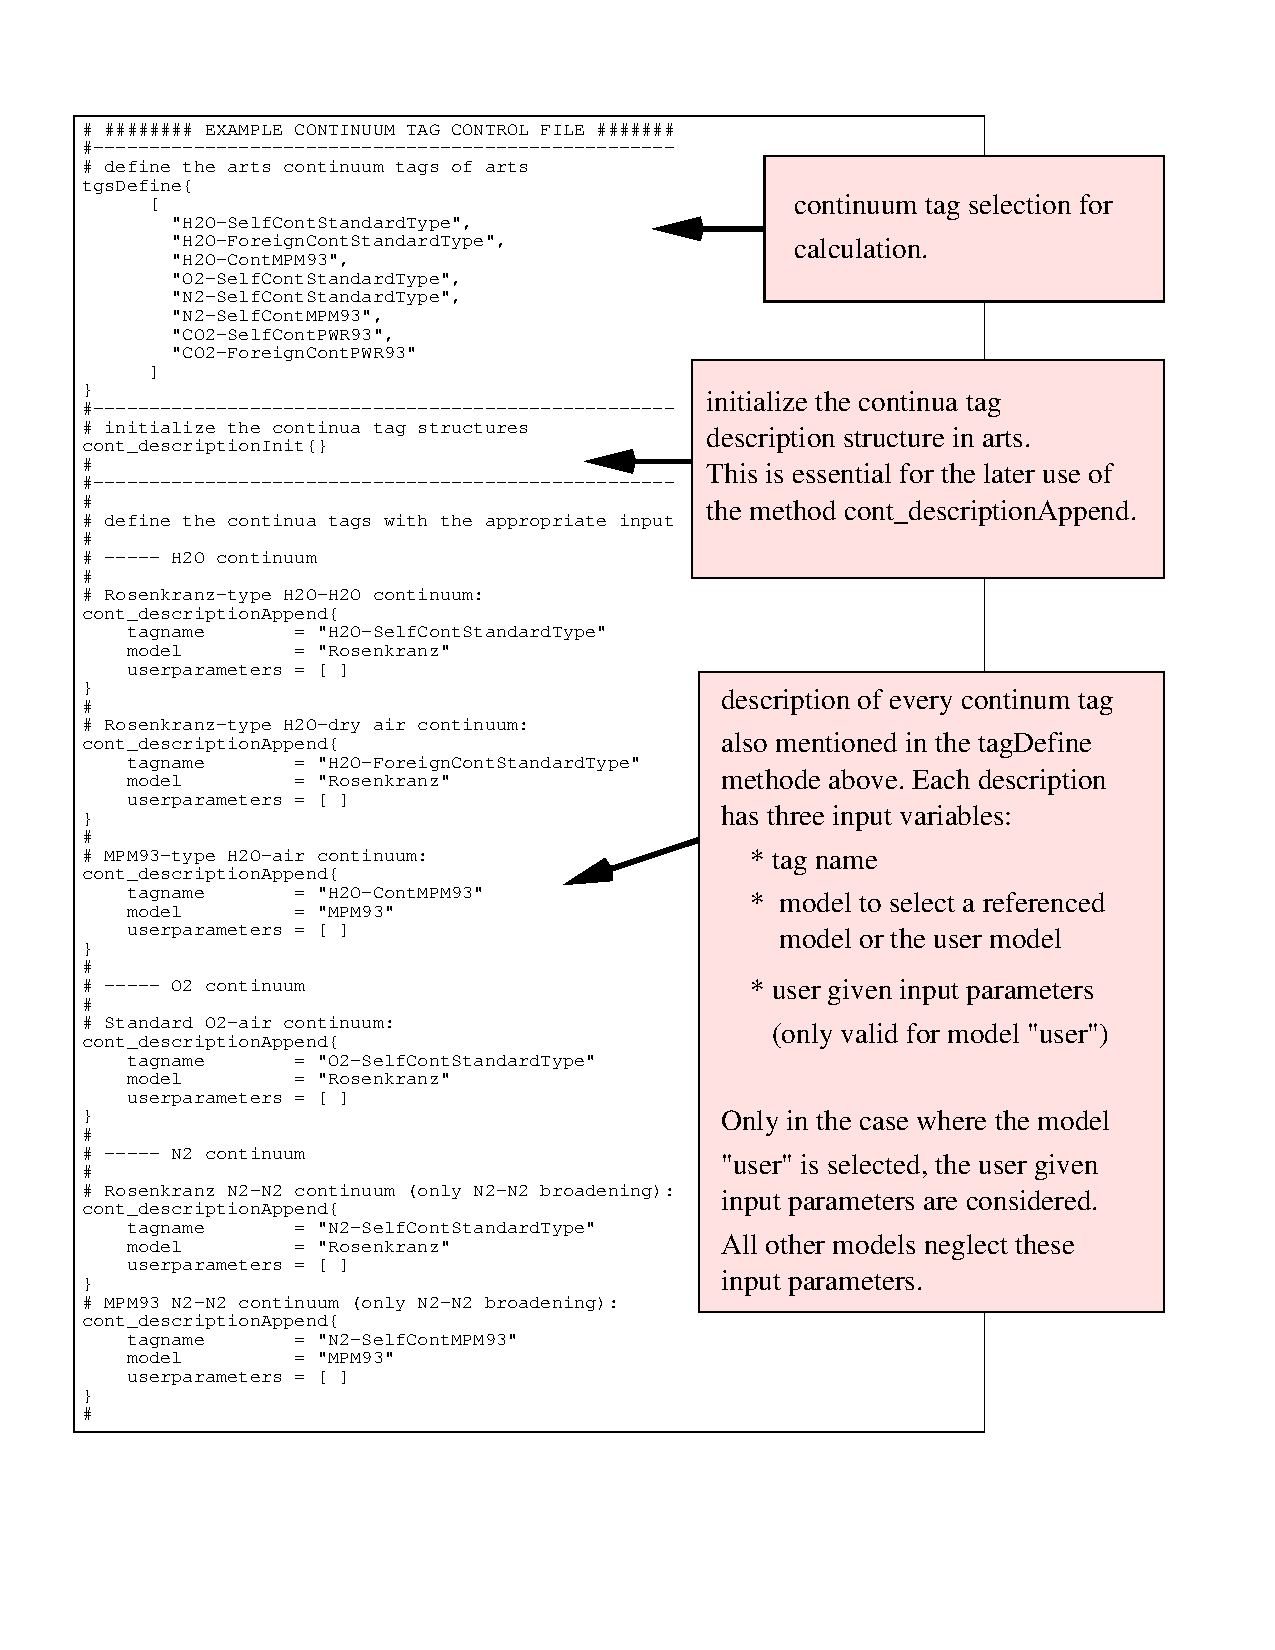
\includegraphics[scale=0.65, angle=0]{cont_description_page1}
\end{flushleft}
\begin{flushleft}
 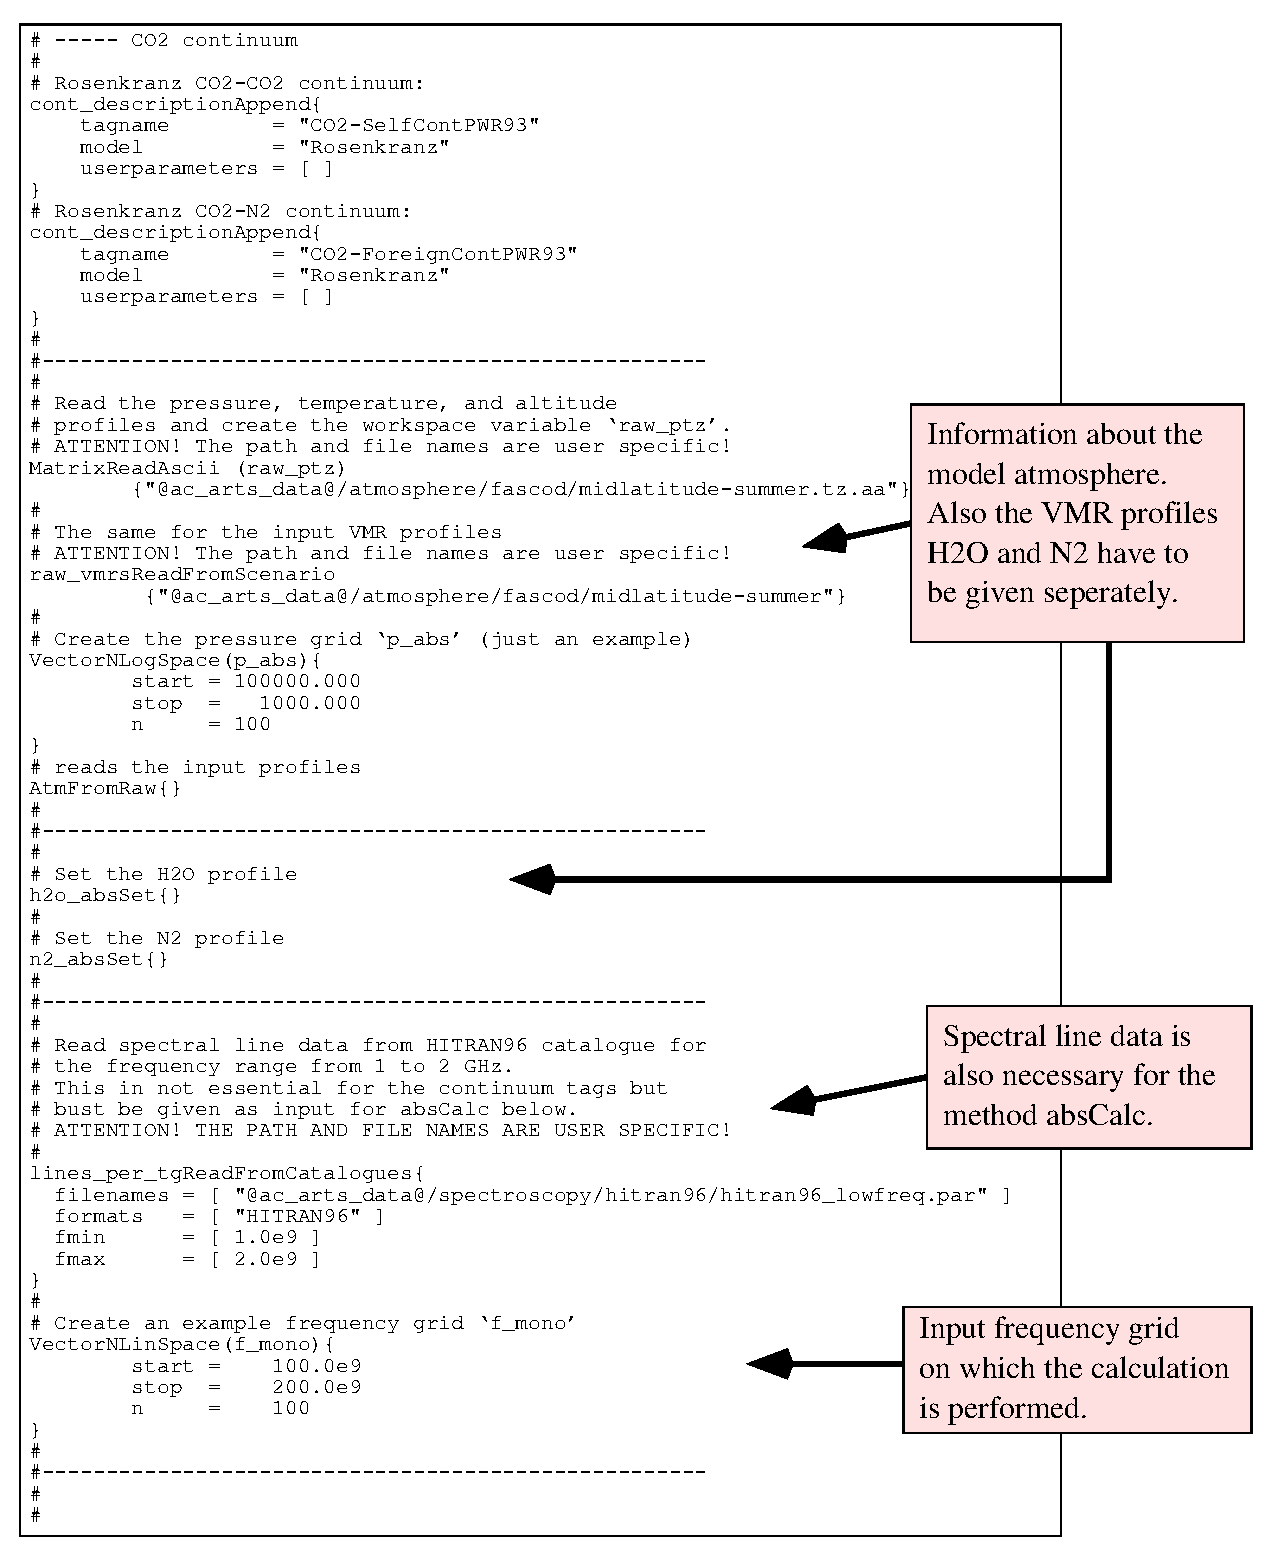
\includegraphics[scale=0.65, angle=0]{cont_description_page2}
\end{flushleft}
\begin{flushleft}
 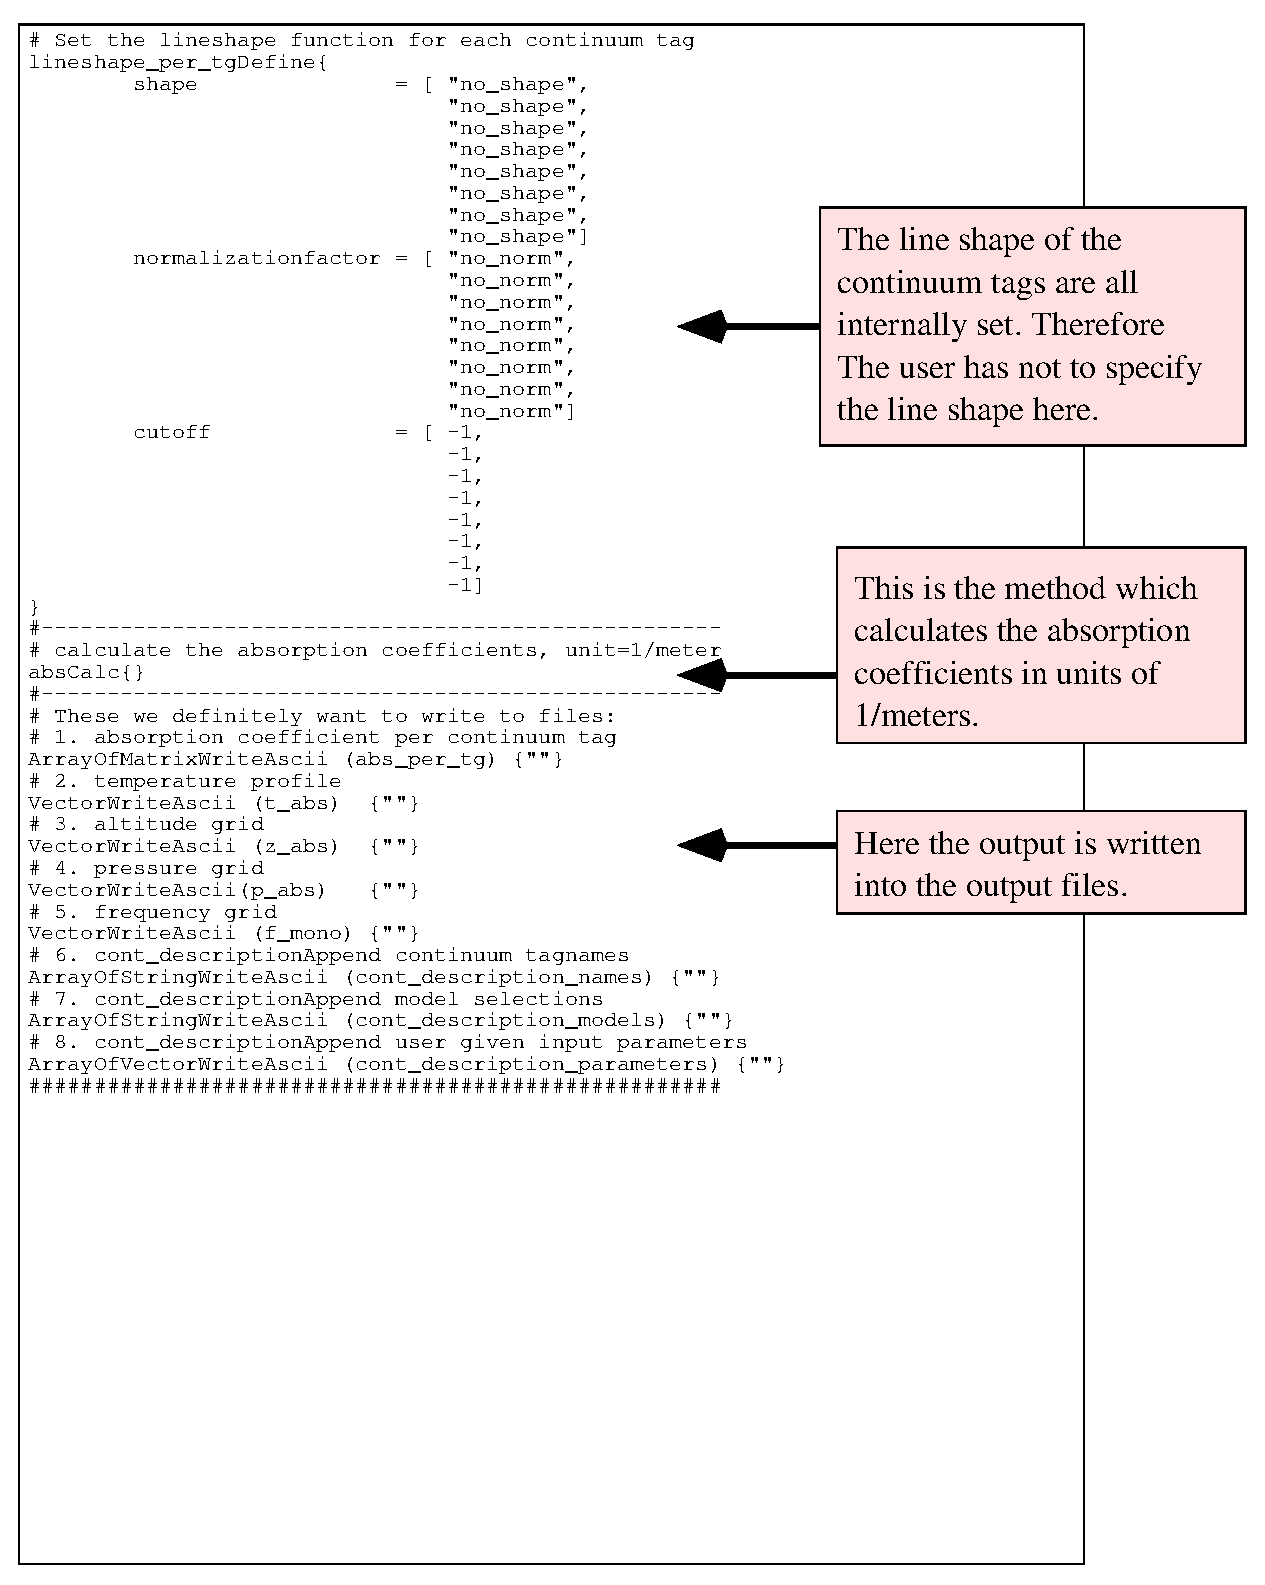
\includegraphics[scale=0.65, angle=0]{cont_description_page3}
\end{flushleft}



% ================================================================================
% The following section is written by Thomas Kuhn, iup Bremen, tkuhn@uni-bremen.de
% ================================================================================



\levelb{Complete Absorption Models}
\label{levelb:CompAbsMod}
% =================================
The MPM absorption model of Liebe and coworkers consists of modules for 
water vapor and oxygen absorption. The Rosenkranz (PWR98) absorption 
model include also $\hzo$ and $\oz$ while the Cruz-Pol et al. (CP98) absorption 
models include absorption due to water vapor. Additionally 
the CP98 model has a strongly reduced parameter set for the $\hzo$-line 
absorption since it is especially intended for the range around the 
22\,GHz water line. The MPM and R98 are valid from the microwave 
up to the submillimeter frequency range (1-1000\,GHz).

Implemented in ARTS are the following modules of the above mentioned models:
%
\begin{center}
\begin{tabular}{ll}
\hline
species & model\\
\hline
$\hzo$ & MPM87, MPM89, MPM93, PWR98, CP98 \\
$\oz$  & MPM93, PWR98 \\
\hline
\end{tabular}
\end{center}




\levelc{Complete Water Vapor Models}
\label{levelc:CompWatVapMod}
% ==================================
In ARTS several complete water vapor absorption models are implemented and 
can easily be used. Implemented models are the versions 
MPM87 \cite{liebeandlayton:87}, MPM89 \cite{liebe:89}, and 
MPM93 \cite{liebeetal:93} of the Liebe Millimeter-wave Propagation Model 
and additionally the models of Cruz-Pol et al. (CP98) \cite{cruzpol:98} 
and P.~W. Rosenkranz (PWR98) \cite{pwr:98}. 
MPM and PWR98 are especially desigend for fast absorption calculations in 
the frequency range of 1-1000\,GHz while the CP98 model is a reduced model 
for a narrow frequency band around the 22\,GHz $\hzo$-line (especially used 
by ground-based radiometers).

The total water vapor absorption ($\alphatot$) is in all the stated models 
described by a line absorption ($\alphal$) term and a continuum absorption 
($\alphac$) term: 
\begin{equation}
  \label{eq:h2o:totabs}
  \alphatot = \alphal + \alphac
\end{equation}
The main differences between the different models is the line shape used for 
$\alphal$ and the formulation of $\alphac$.

It has to be emphasized that, $\alphal$ and $\alphac$ of different
models are not necessarily compatible and should therefore not be 
interchanged between different models.


\leveld{MPM87 Water Vapor Absorption Model}
\label{leveld:mpm87}
%------------------------------------------
This version, which is described in \cite{liebeandlayton:87} and 
follows the general line of the MPM model to divide the total 
water vapor absorption, $\alphampmotot$, into a spectral line 
term, $\alphampmol$, and a continuum term not attributed to 
spectral lines, $\alphampmoc$:
\begin{equation}
  \label{eq:mpm87_abs}
  \alphampmotot = \alphampmol + \alphampmoc\hspace*{10mm}\mbox{dB/km}
\end{equation}



\levele{Water Vapor Line Absorption:}
\label{levele:mpm87_h2olines}
%-----------------------------------
The MPM87 \cite{liebeandlayton:87} water vapor line catalog consists 
of 30 lines from 22\,GHz up to 988\,GHz. The center frequencies and parameter 
values are listed in Table \ref{tab:mpm87linelist}. To describe the line 
absorption, a set of three parameters ($\bek$ and $\bdk$) per line are used: two 
for the line strength and one for the line width. The total line 
absorption coefficient (in units of dB/km) is the sum over all 
individual line absorption coefficients\footnote{The factor 
  $0.1820 \cdot 10^{6}$ is equal to $(4\,\pi/c)\cdot 10\log{(e)}$
  (the term $(4\,\pi/c)$ comes from the definition of the absorption
  coefficient in terms of the dielectric constant and the term 
  $10\,\log{(e)}$ is due to the definition of the Decibel.) The
  velocity of light is defined as $c=2.9979\cdot 10^{-4}$\,km\,GHz. 
  The factor $10^{6}$ is incorporated into the line strength and 
  does therefore not appear in the pre-factor.}:
\begin{equation}
  \label{eq:mpm87:absline}
  \alphampmol = 0.1820 \cdot \nuk \cdot \phzo \cdot 
  \sum_{k}{\inten \cdot \shape}\hspace*{10mm}\mbox{dB/km}
\end{equation}
where $\inten$ is the line intensity described by the parameterization
\begin{equation}
  \label{eq:mpm87:strength}
  \inten = \bek \cdot \phzo \cdot \Theta^{3.5} 
           \cdot \exp{(\bzk \cdot [1-\Theta])}\hspace*{10mm}\mbox{kHz}
\end{equation}
with $\nuk$ as the line center frequency, $\phzo$ the water
vapor partial pressure and $\Theta = 300\,\mbox{K}/T$.\\
The line shape function, $\shape$, in Eq.~(\ref{eq:mpm87:absline}) 
is the standard Van~Vleck-Weisskopf (VVW) function, given by:
\begin{eqnarray}
% Van Vleck-Weisskopf function
  \label{eq:mpm87:VVW}
  \shape & = & \left(\frac{\nu}{\nuk}\right) \cdot 
               \left[\frac{\gamk}{(\nu - \nuk)^2 + \gamk^2} + 
                     \frac{\gamk}{(\nu + \nuk)^2 + \gamk^2}\right]\\
\end{eqnarray}
The pressure broadened line width, $\gamk$, is calculated with the 
single parameter $\bdk$ in the following way:
\begin{equation}
  \label{eq:mpm87:gamma}
  \gamk = \bdk \cdot 
          (4.80 \cdot \phzo \cdot \Theta^{1.1} + \pda \cdot
          \Theta^{0.6})\hspace*{10mm}\mbox{GHz}
\end{equation}
where $\pda$ is the partial pressure of dry air ($\pda=\ptot-\phzo$). 
The parameterizations of $\inten$ and $\gamk$ are already in use for the 
early version of MPM81 \cite{liebe:81}.
%
\begin{longtable}{rrrrr}
 K & K & K & K & K \kill
%
% --------------------- only begin of table ------------------------------
 \hline
       & $\nu_k$ & $\bek$   & $\bzk$ & $\bdk$  \\
% //      [GHz]    [kHz/kPa]   [1]     [GHz/kPa]
 $k$   & {\rm [GHz]}  & {[$\frac{\rm kHz}{\rm kPa}$]} & {\rm [1]} & 
 {[$\frac{\rm GHz}{\rm kPa}$]}\\
 \hline
 \endfirsthead
% --------------------- every page begin of table ------------------------
 \hline
  $k$  & $\nu_k$ & $\bek$ & $\bzk$ & $\bdk$ \\
 \hline
 \endhead
% --------------------- every page end of table ------------------------
 K & K & K & K & K \kill
 \hline
 \caption[]{(continued)}\\
 \endfoot
% --------------------- only end of table ------------------------------
 K & K & K & K & K \kill 
 \hline
 \caption{List of H$_2$O spectral lines and their spectroscopic 
   parameters (H$_2$O-air mixture) for the MPM87 model \cite{liebeandlayton:87}.}
 \label{tab:mpm87linelist}
 \endlastfoot
% --------------------- body of table  ----------------------------------  
% //         0           1           2       3      
% //         f0          b1          b2      b3     
% //        [GHz]       [kHz/kPa]   [1]    [GHz/kPa]
%  const Numeric mpm87[30][4] = { 
1     &    22.235080&    0.1090&  2.143&   27.84$\cdot$ 10$^{-3}$\\
2     &    67.813960&    0.0011&  8.730&   27.60$\cdot$ 10$^{-3}$\\
3     &   119.995940&    0.0007&  8.347&   27.00$\cdot$ 10$^{-3}$\\
4     &   183.310117&    2.3000&  0.653&   31.64$\cdot$ 10$^{-3}$\\
5     &   321.225644&    0.0464&  6.156&   21.40$\cdot$ 10$^{-3}$\\
6     &   325.152919&    1.5400&  1.515&   29.70$\cdot$ 10$^{-3}$\\
7     &   336.187000&    0.0010&  9.802&   26.50$\cdot$ 10$^{-3}$\\
8     &   380.197372&   11.9000&  1.018&   30.36$\cdot$ 10$^{-3}$\\
9     &   390.134508&    0.0044&  7.318&   19.00$\cdot$ 10$^{-3}$\\
10    &   437.346667&    0.0637&  5.015&   13.70$\cdot$ 10$^{-3}$\\
11    &   439.150812&    0.9210&  3.561&   16.40$\cdot$ 10$^{-3}$\\
12    &   443.018295&    0.1940&  5.015&   14.40$\cdot$ 10$^{-3}$\\
13    &   448.001075&   10.6000&  1.370&   23.80$\cdot$ 10$^{-3}$\\
14    &   470.888947&    0.3300&  3.561&   18.20$\cdot$ 10$^{-3}$\\
15    &   474.689127&    1.2800&  2.342&   19.80$\cdot$ 10$^{-3}$\\
16    &   488.491133&    0.2530&  2.814&   24.90$\cdot$ 10$^{-3}$\\
17    &   503.568532&    0.0374&  6.693&   11.50$\cdot$ 10$^{-3}$\\
18    &   504.482692&    0.0125&  6.693&   11.90$\cdot$ 10$^{-3}$\\
19    &   556.936002&  510.0000&  0.114&   30.00$\cdot$ 10$^{-3}$\\
20    &   620.700807&    5.0900&  2.150&   22.30$\cdot$ 10$^{-3}$\\
21    &   658.006500&    0.2740&  7.767&   30.00$\cdot$ 10$^{-3}$\\
22    &   752.033227&  250.0000&  0.336&   28.60$\cdot$ 10$^{-3}$\\
23    &   841.073593&    0.0130&  8.113&   14.10$\cdot$ 10$^{-3}$\\
24    &   859.865000&    0.1330&  7.989&   28.60$\cdot$ 10$^{-3}$\\
25    &   899.407000&    0.0550&  7.845&   28.60$\cdot$ 10$^{-3}$\\
26    &   902.555000&    0.0380&  8.360&   26.40$\cdot$ 10$^{-3}$\\
27    &   906.205524&    0.1830&  5.039&   23.40$\cdot$ 10$^{-3}$\\
28    &   916.171582&    8.5600&  1.369&   25.30$\cdot$ 10$^{-3}$\\
29    &   970.315022&    9.1600&  1.842&   24.00$\cdot$ 10$^{-3}$\\
30    &   987.926764&  138.0000&  0.178&   28.60$\cdot$ 10$^{-3}$\\
\hline
% -----------------------------------------------------------------------  
\end{longtable}


\levele{Water Vapor Continuum Absorption:}
\label{levele:mpm87_h2ocont}
%----------------------------------------
The water vapor continuum absorption coefficient in MPM87, $\alphampmoc$, 
is determined from laboratory measurements at 137.8\,GHz by Liebe 
and Layton covering the following parameter range:\\
\begin{tabular}{lr}
temperature          & 282-316\,K\\
relative humidity    & 0-95\,\%\\
dry air pressure     & 0 - 160\,kPa\\ 
\end{tabular}\\
The mathematical expression of $\alphampmoc$ is derived from the far wing 
approximation of the line absorption and is expressed as follows
\begin{equation} 
  \label{eq:mpm87:cont}
  \alphampmoc = \nu^2 \cdot \phzo \cdot 
                (\cso \cdot \phzo \cdot \Theta^{\xs} + 
                 \cdo \cdot \pda  \cdot \Theta^{\xf}),
\end{equation}
with the continuum parameter set $\cso$, $\cdo$, $\xs$, and $\xf$. 
The determined values of the continuum parameters are:

\begin{description}
\item{$\cso$}   =  6.496\,$\cdot$\,10$^{-6}$~~(dB/km)~/~(hPa$\cdot$GHz)$^2$
\item{$\xs$}    = 10.5
\item{$\cdo$}   =  0.206\,$\cdot$\,10$^{-6}$~~(dB/km)~/~(hPa$\cdot$GHz)$^2$
\item{$\xd$}    =  3.0
\end{description}




\leveld{MPM89 Water Vapor Absorption Model}
\label{leveld:mpm89}
%------------------------------------------
%
MPM89 is described in \cite{liebe:89} and follows the general line 
of the MPM model to devide the total water vapor absorption, 
$\alphampmmtot$, into a spectral line term, $\alphampmml$, and a continuum 
term not attributed to spectral lines, $\alphampmmc$:
\begin{equation}
  \label{eq:mpm89_abs}
  \alphampmmtot = \alphampmml + \alphampmmc\hspace*{10mm}\mbox{dB/km}
\end{equation}
All the absorption coefficients are calculated in units of \mbox{dB/km}.


\levele{Water Vapor Line Absorption:}
\label{levele:mpm89_h2olines}
%-----------------------------------
The MPM89 water vapor line catalog consists of the same 30 lines 
like MPM87 from 22\,GHz up to 988\,GHz. The center frequencies and parameter 
values are listed in Table \ref{tab:mpm89linelist}. To describe the line 
absorption, a set of six parameters ($\bek$ and $\bsk$) per line are used: two 
for the line strength and four for the line width. The total line 
absorption coefficient (in units of dB/km) is the sum over all
individual line absorption coefficients\footnote{see footnote for
  MPM97 line absorption}:
\begin{equation}
  \label{eq:mpm89:absline}
  \alphampmml = 0.1820 \cdot \nuk \cdot \phzo \cdot 
  \sum_{k}{\inten \cdot \shape}\hspace*{10mm}\mbox{dB/km}
\end{equation}
where $\inten$ is the line intensity described by the parameterization
\begin{equation}
  \label{eq:mpm89:strength}
  \inten = \bek \cdot \phzo \cdot \Theta^{3.5} 
           \cdot \exp{(\bzk \cdot [1-\Theta])}\hspace*{10mm}\mbox{kHz}
\end{equation}
whit $\nuk$ as the line center frequency, $\phzo$ the water
vapor partial pressure and $\Theta = 300\,\mbox{K}/T$.\\
The line shape function, $\shape$, in Eq.~(\ref{eq:mpm89:absline}) 
is the standard Van Vleck-Weisskopf (VVW) function, given by 
\begin{eqnarray}
% Van Vleck-Weisskopf function
  \label{eq:mpm89:VVW}
  \shape & = & \left(\frac{\nu}{\nuk}\right) \cdot 
               \left[\frac{\gamk}{(\nu - \nuk)^2 + \gamk^2} + 
                     \frac{\gamk}{(\nu + \nuk)^2 + \gamk^2}\right]
\end{eqnarray}
where the pressure broadened line width, $\gamk$, is calculated as
\begin{equation}
  \label{eq:mpm89:gamma}
  \gamk = \bdk \cdot 
         (\bfk \cdot \phzo \cdot \Theta^{\bsk} + 
                     \pda  \cdot \Theta^{\bvk})
        \cdot 10^{-3}\hspace*{10mm}\mbox{GHz}
\end{equation}
with $\pda=\ptot-\phzo$ as the dry air partial pressure. 
The only difference between MPM87 and MPM89 with respect to the line 
absorption is the parameterization of the pressure broadened line
width, $\gamk$, which is calculated with the four parameters $\bdk$ to
$\bsk$ in the case of MPM89 whereas in MPM87 a single parameter
($\bdk$) is used (see Eq.~(\ref{eq:mpm87:gamma})).
%
\begin{longtable}{rrrrrrrr}
 K & K & K & K & K & K & K & K \kill
%
% --------------------- only begin of table ------------------------------
 \hline
    & $\nu_k$ & $\bek$ & $\bzk$ & $\bdk$ & $\bvk$ & $\bfk$ & $\bsk$ \\
%    [GHz]     [kHz/kPa]   [1]   [MHz/kPa]  [1]    [1]    [1]
 $k$& {\rm [GHz]}  & {[$\frac{\rm kHz}{\rm kPa}$]} & {\rm [1]} & 
 {[$\frac{\rm MHz}{\rm kPa}$]} & {\rm [1]} & {\rm [1]} & {\rm [1]} \\
 \hline
 \endfirsthead
% --------------------- every page begin of table ------------------------
 \hline
  $k$  & $\nu_k$ & $\bek$ & $\bzk$ & $\bdk$ & $\bvk$ & $\bfk$ & $\bsk$ \\
 \hline
 \endhead
% --------------------- every page end of table ------------------------
 K & K & K & K & K & K & K & K \kill
 \hline
 \caption[]{(continued)}\\
 \endfoot
% --------------------- only end of table ------------------------------
 K & K & K & K & K & K & K & K \kill
 \hline
 \caption{List of H$_2$O spectral lines and their spectroscopic 
   parameters (H$_2$O-air mixture) for the MPM89 model \cite{liebe:89}.}
 \label{tab:mpm89linelist}
 \endlastfoot
% --------------------- body of table  ----------------------------------  
%            0           1        2       3        4      5      6
%            f0          b1       b2      b3       b4     b5     b6
%          [GHz]     [kHz/kPa]   [1]   [MHz/kPa]  [1]    [1]    [1]
%  const Numeric mpm89[30][7] = { 
1    &    22.235080&    0.1090&  2.143&   28.11&   0.69&  4.80&  1.00\\
2    &    67.813960&    0.0011&  8.735&   28.58&   0.69&  4.93&  0.82\\
3    &   119.995940&    0.0007&  8.356&   29.48&   0.70&  4.78&  0.79\\
4    &   183.310074&    2.3000&  0.668&   28.13&   0.64&  5.30&  0.85\\
5    &   321.225644&    0.0464&  6.181&   23.03&   0.67&  4.69&  0.54\\
6    &   325.152919&    1.5400&  1.540&   27.83&   0.68&  4.85&  0.74\\
7    &   336.187000&    0.0010&  9.829&   26.93&   0.69&  4.74&  0.61\\
8    &   380.197372&   11.9000&  1.048&   28.73&   0.69&  5.38&  0.84\\
9    &   390.134508&    0.0044&  7.350&   21.52&   0.63&  4.81&  0.55\\
10    &   437.346667&    0.0637&  5.050&   18.45&   0.60&  4.23&  0.48\\
11    &   439.150812&    0.9210&  3.596&   21.00&   0.63&  4.29&  0.52\\
12    &   443.018295&    0.1940&  5.050&   18.60&   0.60&  4.23&  0.50\\
13    &   448.001075&   10.6000&  1.405&   26.32&   0.66&  4.84&  0.67\\
14    &   470.888947&    0.3300&  3.599&   21.52&   0.66&  4.57&  0.65\\
15    &   474.689127&    1.2800&  2.381&   23.55&   0.65&  4.65&  0.64\\
16    &   488.491133&    0.2530&  2.853&   26.02&   0.69&  5.04&  0.72\\
17    &   503.568532&    0.0374&  6.733&   16.12&   0.61&  3.98&  0.43\\
18    &   504.482692&    0.0125&  6.733&   16.12&   0.61&  4.01&  0.45\\
19    &   556.936002&  510.0000&  0.159&   32.10&   0.69&  4.11&  1.00\\
20    &   620.700807&    5.0900&  2.200&   24.38&   0.71&  4.68&  0.68\\
21    &   658.006500&    0.2740&  7.820&   32.10&   0.69&  4.14&  1.00\\
22    &   752.033227&  250.0000&  0.396&   30.60&   0.68&  4.09&  0.84\\
23    &   841.073593&    0.0130&  8.180&   15.90&   0.33&  5.76&  0.45\\
24    &   859.865000&    0.1330&  7.989&   30.60&   0.68&  4.09&  0.84\\
25    &   899.407000&    0.0550&  7.917&   29.85&   0.68&  4.53&  0.90\\
26    &   902.555000&    0.0380&  8.432&   28.65&   0.70&  5.10&  0.95\\
27    &   906.205524&    0.1830&  5.111&   24.08&   0.70&  4.70&  0.53\\
28    &   916.171582&    8.5600&  1.442&   26.70&   0.70&  4.78&  0.78\\
29    &   970.315022&    9.1600&  1.920&   25.50&   0.64&  4.94&  0.67\\
30    &   987.926764&  138.0000&  0.258&   29.85&   0.68&  4.55&  0.90\\
\hline
% -----------------------------------------------------------------------  
\end{longtable}


\levele{Water Vapor Continuum Absorption:}
\label{levele:mpm89_h2ocont}
%----------------------------------------
The MPM89 continuum absorption coefficients in, $\alphampmmc$, 
are identical as those in MPM87 (see Sec. \ref{levele:mpm87_h2ocont} for 
details):
\begin{equation} 
  \label{eq:mpm89:cont}
  \alphampmmc = \nu^2 \cdot \phzo \cdot 
                (\cso \cdot \phzo \cdot \Theta^{\xs} + 
                 \cdo \cdot \pda  \cdot \Theta^{\xf}),
\end{equation}
with
\begin{description}
\item{$\cso$}   =  6.496\,$\cdot$\,10$^{-6}$~~(dB/km)~/~(hPa$\cdot$GHz)$^2$
\item{$\xs$}    = 10.5
\item{$\cdo$}   =  0.206\,$\cdot$\,10$^{-6}$~~(dB/km)~/~(hPa$\cdot$GHz)$^2$
\item{$\xd$}    =  3.0
\end{description}





\leveld{MPM93 Water Vapor Absorption Model}
\label{leveld:mpm93}
%----------------------------------------------
This version, which is described in \cite{liebeetal:93} and 
follows the general line of the MPM model to devide the total 
water vapor absorption, $\alphampmntot$, into a spectral line 
term, $\alphampmnl$, and a continuum term not attributed to 
spectral lines, $\alphampmnc$:
\begin{equation}
  \label{eq:mpm93_abs}
  \alphampmntot = \alphampmnl + \alphampmnc\hspace*{10mm}\mbox{dB/km}
\end{equation}
The continuum absorption is parameterized like a
resonant spectral line of $\hzo$, a so-called pseudo-line. This is a 
fundamental change in the parameterization of the water vapor
continuum in respect to all older versions of MPM, which makes it 
quite complicate to compare the different versions, especially to 
distinguish a self- and foreign broadening term in the continuum.



\levele{Water Vapor Line Absorption:}
\label{levele:mpm93_h2olines}
%-----------------------------------
The water vapor line spectrum of MPM93 \cite{liebeetal:93} 
consists of 34 lines below 1\,THz (four more than in MPM89 and MPM87). 
To describe the MPM93 water vapor line absorption, a set of six parameters 
($\bek$ and $\bdk$) per line are used: two for the line strength and 
four for the line width. The total line absorption coefficient 
(in units of dB/km) is the sum over all individual line absorption 
coefficients\footnote{see footnote for MPM97 line absorption}:
\begin{equation}
  \label{eq:mpm93:absline}
  \alphampmnl = 0.1820 \cdot \nuk \cdot \phzo \cdot 
  \sum_{k}{\inten \cdot \shape}\hspace*{10mm}\mbox{dB/km}
\end{equation}
where $\inten$ is the line intensity described by the parameterization
\begin{equation}
  \label{eq:mpm93:strength}
  \inten = \bek \cdot \phzo \cdot \Theta^{3.5} 
           \cdot \exp{(\bzk \cdot [1-\Theta])}\hspace*{10mm}\mbox{kHz}
\end{equation}
with $\nuk$ as the line center frequency, $\phzo$ the water
vapor partial pressure and $\Theta = 300\,\mbox{K}/T$.\\
The line shape function, $\shape$, in Eq.~(\ref{eq:mpm87:absline}) 
is the standard Van~Vleck-Weisskopf (VVW) function, given by:
\begin{eqnarray}
% Van Vleck-Weisskopf function
  \label{eq:mpm93:VVW}
  \shape & = & \left(\frac{\nu}{\nuk}\right) \cdot 
               \left[\frac{\gamk}{(\nu - \nuk)^2 + \gamk^2} + 
                     \frac{\gamk}{(\nu + \nuk)^2 + \gamk^2}\right]\\
\end{eqnarray}
The pressure broadened line width, $\gamk$, is calculated with the 
single parameter $\bdk$ in the following way:
\begin{equation}
  \label{eq:mpm93:gamma}
  \gamk = \bdk \cdot 
          (4.80 \cdot \phzo \cdot \Theta^{1.1} + \pda \cdot
          \Theta^{0.6})\hspace*{10mm}\mbox{GHz}
\end{equation}
where $\pda$ is the partial pressure of dry air ($\pda=\ptot-\phzo$). 

The parameterizations of $\inten$ was already in use for the early 
version of MPM81 \cite{liebe:81}. The expression for $\gamk$ is the
same as in MPM89. The main difference between MPM93 and MPM89 
concerning the water vapor line absorption is the updated line catalog.
%
%
%\begin{landscape}
%\setlength{\LTcapwidth}{200mm} % with of the caption in longtable
\begin{longtable}{rrrrrrrr}
 K & K & K & K & K & K & K & K \kill
%
% --------------------- only begin of table ------------------------------
 \hline
       & $\nu_k$ & $\bek$ & $\bzk$ & $\bdk$ & $\bvk$ & $\bfk$ & $\bsk$ \\
 $k$   & {\rm [GHz]}  & {[$\frac{\rm kHz}{\rm hPa}$]} & {\rm [1]} & 
 {[$\frac{\rm MHz}{\rm hPa}$]} & {\rm [1]} & {\rm [1]} & {\rm [1]} \\
 \hline
 \endfirsthead
% --------------------- every page begin of table ------------------------
 \hline
    & $\nu_k$ & $\bek$ & $\bzk$ & $\bdk$ & $\bvk$ & $\bfk$ & $\bsk$ \\
 \hline
 \endhead
% --------------------- every page end of table ------------------------
 K & K & K & K & K & K & K & K \kill
 \hline
 \caption[]{(continued)}\\
 \endfoot
% --------------------- only end of table ------------------------------
 K & K & K & K & K & K & K & K \kill
 \hline
 \caption{List of used H$_2$O spectral lines and their spectroscopic 
   coefficients of H$_2$O in air for the MPM93 model \citep{liebeetal:93}. 
   The last separated line is the unphysical pseudo-line used in MPM93. 
   The lines which are marked with a "$^+$" were not in the MPM87/MPM89 
   line catalog.}
 \label{tab:mpm93linelist}
 \endlastfoot
% --------------------- body of table  ----------------------------------  
1      & 22.235080  & 0.01130 & 2.143 & 2.811 & 4.80 & 0.69 & 1.00 \\
2      & 67.803960  & 0.00012 & 8.735 & 2.858 & 4.93 & 0.69 & 0.82 \\
3      & 119.995940 & 0.00008 & 8.356 & 2.948 & 4.78 & 0.70 & 0.79 \\
4      & 183.310091 & 0.24200 & 0.668 & 3.050 & 5.30 & 0.64 & 0.85 \\
5      & 321.225644 & 0.00483 & 6.181 & 2.303 & 4.69 & 0.67 & 0.54 \\ 
6      & 325.152919 & 0.14990 & 1.540 & 2.783 & 4.85 & 0.68 & 0.74 \\
7      & 336.222601 & 0.00011 & 9.829 & 2.693 & 4.74 & 0.69 & 0.61 \\ 
8      & 380.197372 & 1.15200 & 1.048 & 2.873 & 5.38 & 0.54 & 0.89 \\
9      & 390.134508 & 0.00046 & 7.350 & 2.152 & 4.81 & 0.63 & 0.55 \\
10     & 437.346667 & 0.00650 & 5.050 & 1.845 & 4.23 & 0.60 & 0.48 \\
11     & 439.150812 & 0.09218 & 3.596 & 2.100 & 4.29 & 0.63 & 0.52 \\
12     & 443.018295 & 0.01976 & 5.050 & 1.860 & 4.23 & 0.60 & 0.50 \\
13     & 448.001075 & 1.03200 & 1.405 & 2.632 & 4.84 & 0.66 & 0.67 \\
14     & 470.888947 & 0.03297 & 3.599 & 2.152 & 4.57 & 0.66 & 0.65 \\
15     & 474.689127 & 0.12620 & 2.381 & 2.355 & 4.65 & 0.65 & 0.64 \\
16     & 488.491133 & 0.02520 & 2.853 & 2.602 & 5.04 & 0.69 & 0.72 \\
17     & 503.568532 & 0.00390 & 6.733 & 1.612 & 3.98 & 0.61 & 0.43 \\
18     & 504.482692 & 0.00130 & 6.733 & 1.612 & 4.01 & 0.61 & 0.45 \\
19$^+$ & 547.676440 & 0.97010 & 0.114 & 2.600 & 4.50 & 0.70 & 1.00 \\
20$^+$ & 552.020960 & 1.47700 & 0.114 & 2.600 & 4.50 & 0.70 & 1.00 \\
21     & 556.936002 & 48.74000& 0.159 & 3.210 & 4.11 & 0.69 & 1.00 \\
22     & 620.700807 & 0.50120 & 2.200 & 2.438 & 4.68 & 0.71 & 0.68 \\
23$^+$ & 645.866155 & 0.00713 & 8.580 & 1.800 & 4.00 & 0.60 & 0.50 \\
24     & 658.005280 & 0.03022 & 7.820 & 3.210 & 4.14 & 0.69 & 1.00 \\
25     & 752.033227 & 23.96000& 0.396 & 3.060 & 4.09 & 0.68 & 0.84 \\
26     & 841.053973 & 0.00140 & 8.180 & 1.590 & 5.76 & 0.33 & 0.45 \\
27     & 859.962313 & 0.01472 & 7.989 & 3.060 & 4.09 & 0.68 & 0.84 \\
28     & 899.306675 & 0.00605 & 7.917 & 2.985 & 4.53 & 0.68 & 0.90 \\
29     & 902.616173 & 0.00426 & 8.432 & 2.865 & 5.10 & 0.70 & 0.95 \\
30     & 906.207325 & 0.01876 & 5.111 & 2.408 & 4.70 & 0.70 & 0.53 \\
31     & 916.171582 & 0.83400 & 1.442 & 2.670 & 4.78 & 0.70 & 0.78 \\
32$^+$ & 923.118427 & 0.00869 & 10.220& 2.900 & 5.00 & 0.70 & 0.80 \\
33     & 970.315022 & 0.89720 & 1.920 & 2.550 & 4.94 & 0.64 & 0.67 \\
34     & 987.926764 & 13.21000& 0.258 & 2.985 & 4.55 & 0.68 & 0.90 \\
\hline
 & $\nu^*$ & $\beks$ & $\bzks$ & $\bdks$ & $\bvks$ & $\bfks$ & $\bsks$\\
 & {\rm [GHz]}  & {[$\frac{\rm kHz}{\rm hPa}$]} & {\rm [1]} & 
 {[$\frac{\rm MHz}{\rm hPa}$]} & {\rm [1]} & {\rm [1]} & {\rm [1]} \\
\hline
 & 1780.000000 & 2230.00000 & 0.952 & 17.620 & 30.50 & 2.00 & 5.00 \\
% -----------------------------------------------------------------------  
\end{longtable}
%\setlength{\LTcapwidth}{0.8\textwidth}
%\end{landscape}



\levele{The MPM93 Continuum Parameterization:}
\label{levele:mpm93:h2ocont}
%-----------------------------------------------
In the MPM93 version the water vapor continuum is parameterized as an
ordinary spectral line (Eqs. (\ref{eq:mpm93:strength}, 
\ref{eq:mpm93:VVW})). The parameters of this continuum "pseudo-line" 
($\nu^*$, $\beks$, $\bzks$, $\bdks$, $\bvks$, $\bfks$, $\bsks$) 
are given in Table \ref{tab:mpm93linelist}. More details about 
this continuum parameterization and its microwave approximation can be 
found in Section \ref{leveld:h2o_Cont} of this guide.




\leveld{CP98 Water Vapor Absorption Model}
\label{leveld:cp98}
%---------------------------------------------

\levele{Line Absorption}
\label{levele:cp98_h2oline}
%--------------------------
component \citep{cruzpol:98} for the water vapor line absorption 
is based on MPM87 with the main difference that the 
line catalog consists of only a single line at $\nu_{\rm o}=$\,22\,GHz. 
The contributions from the other lines is put into the water vapor 
continuum module. The line absorption is therefore very quickly 
calculated (in units of Np/km) according to the formula
\begin{eqnarray}
  \label{eq:cp98:lineabs}
  \alphacpl &=& 0.0419 \cdot \intencp \cdot \shape \\
  \mbox{with} & & \nonumber\\
  \label{eq:cp98:inten}
  \intencp    &=& 0.0109 \cdot C_L \cdot \phzo \cdot \nuo \cdot \Theta^{3.5} 
             \cdot \exp{(2.143\cdot[1-\Theta])}\nonumber\\
%
  \label{eq:cp98:width}
  \gamma &=& 0.002784 \cdot C_W \cdot (\pda \cdot \Theta^{0.6}+ 
             4.8 \cdot \phzo \cdot \Theta^{1.1}) \nonumber\\
\end{eqnarray}
where $\phzo$ and $\pda$ are the partial pressure of water vapor and dry
air in units of hPa, respectively and the Van Vleck-Weisskopf line
shape, $\shape$. The numbers correspond to the line
parameters form MPM87 for this special line and the factors  
$C_L$ and $C_W$ are adjustable scaling factors to match the model with the
measurements. Setting the scaling factors to $C_L$=1.00 and $C_W$=1.00 
leads to the same results as for MPM87. According to the parameter 
estimation of Cruz--Pol et al. best agreement between 
data and model is obtained with $C_L=$\,1.0639$\pm$0.016 and 
$C_W=$\,1.0658$\pm$0.0096. The correlation between these two scaling 
factors was found to be negligible, as can be seen from 
Table \ref{tab:cp_orr}.

\begin{table}[!htb]
\begin{center}
\begin{tabular}{lllll}
\hline
            & $C_L$ & $C_W$ & $C_C$ & $C_X$ \\
\hline
value       & 1.0639 & 1.0658 & 1.2369 & 1.0739\\
std. dev.   & 0.016  & 0.0096 & 0.155  & 0.252\\
\hline
correlation & &&&\\
$C_L$       & 1      & -0.085 & 0.045  & -0.048\\
$C_W$       & -0.085 & 1      & -0.513 &  0.485\\
$C_C$       & 0.045  & -0.513 & 1      & -0.989\\
$C_X$       & -0.048 & 0.485  & -0.989 & 1\\
\hline
\end{tabular}
\end{center}
\caption{Scaling parameter values with standard deviation and 
  correlation coefficients according to \citep{cruzpol:98}.
  The scaling parameters are $C_L$:22\,GHz line strength, 
  $C_W$:22\,GHz line width , $C_C$:$\hzo$-continuum, and 
  $C_X$:$\oz$-absorption. $C_X$ scales the entire oxygen absorption, 
  the continuum as well as the line absorption. The Cruz-Pol et al.
  model uses the \cite{pwr:93} oxygen absorption model.}
\label{tab:cp_orr}
\end{table}

The main reason why the Cruz-Pol model (CP98) considers only one line
lies in the fact that CP98 is especially designed for the data analysis
in the 20-31.4\,GHz region. The determination of the scaling factors was 
performed with ground based radiometer data in the frequency range of
from different locations\footnote{The data were recorded at San Diego, 
California (11. December 1991) and West Palm Beach, Florida 
(8.-21. March 1992)} in the USA.


\levele{Water Vapor Continuum Absorption:}
\label{levele:cp98_h2ocont}
%-----------------------------------------
The CP98 model uses the same water vapor continuum 
parameterization as MPM87, just scaled with an empirical 
factor, $CC$, determined from the above mentioned data:
\begin{equation}
 \label{eq:cp98_cont_scaling}
 \alphacpc = C_C \cdot \alphampmoc 
\end{equation}
The scaling factor $C_C$, as given in Table \ref{tab:cp_orr}, 
gives a 23.69\,\% increased continuum absorption compared 
with MPM87 (see Table \ref{tab:wvcontparam} for a comparison of the 
parameter values). But one has to keep in mind that $C_C$ has a 
high correlation with the scaling factor of the oxygen 
absorption, $C_X$, since these two components could not 
be completely distinguished in the data. Therefore the 
value of 23.69\,\% has a standard deviation of 15.5\,\% 
and is not so reliable than $C_L$ and $C_W$.





\leveld{PWR98 Water Vapor Absorption Model}
\label{leveld:pwr98_h2o}
%------------------------------------------
The water vapor continuum formulation of \citet{pwr:98} is a re-investigation 
of the existing models MPM87/MPM89, MPM93, and CKD\_2.1 especially for 
the frequency region below 1-1000\,GHz. in the context of the available
laboratory and atmospheric data \citep{abaueretal:89, abaueretal:93, 
abaueretal:95, beckerautler:46, englishetal:94, godonetal:92,
liebe:84, liebeandlayton:87, westwateretal:90}.

Rosenkranz adopted the structure of MPM89 for his improved model (R98). 
However, some important differences exist compared with MPM89:
\begin{itemize}
\item the water vapor line catalogs are different 
\item the R98 uses the Van~Vleck--Weisskopf line shape function with 
      cutoff and MPM89 without cutoff
\end{itemize}


\levele{Water Vapor Line Absorption:}
\label{levele:pwr98_h2oline}
%------------------------------------
The local line absorption is defined as 
\begin{eqnarray} 
 \label{eq:pwr98absline}
 \alphapwrl &=& N_{H_2O} \cdot \sum_k \inten \cdot \shapec \nonumber\\
            &=& N_{H_2O} \cdot \sum_k \inten \cdot 
                \left (\displaystyle{\frac{\nu}{\nuk}}\right )^2  \cdot 
                \left [\shapefp + \shapefm \right]~~\mbox{Np/km}
\end{eqnarray}
where $N_{H_2O}$ is the number density of water molecules, $\nu$ the
frequency and $S$ the line intensity, calculated from the HITRAN92
data base \citet{rothman:92}. Considered for this re-investigation are 
15 lines with a frequency lower than 1\,THz as listed in 
Table \ref{tab:pwr98linelist}.

The line shape function $\shapec$ has a cutoff frequency, $\nucut$,
and a baseline subtraction similar to the CKD model \cite{clough:89}.
The introduction of a cutoff frequency has two advantages: (1) the
cutoff avoids applying the line shape to distant frequencies where the 
line form is theoretically not well understood and (2) the cutoff also
establishes a limit to the summation in Eq.~(\ref{eq:pwr98absline}) where lines
far away from the cutoff limit do not contribute to the sum.  
The Rosenkranz formulation uses the same value for
the cutoff frequency as the CKD model:
\begin{equation} 
 \label{cutoff}
 \nucut = 750\mbox{ GHz}
\end{equation}
%
The explicit mathematical form of the line shape function is defined 
in such a way that in the limit $\nucut \rightarrow \infty$ the 
combination of Eq.~(\ref{eq:pwr98absline}) with the line shape function would 
be equivalent to a Van Vleck--Weisskopf \citep{vanvleck:45} line shape: 
\begin{equation}
 \label{eq:pwr98lineshape}
 \hspace*{-8mm}\shapefpm = 
   \left \{ \begin{array}{r@{\quad:\quad}l} 
   \displaystyle{\frac{\gamk}{\pi}} 
   \left \{ \displaystyle{\frac{1}{(\nu \mp \nuk)^2 + \gamk^2}} - 
   \displaystyle{\frac{1}{\nucut^2 + \gamk^2}} \right \}
   & |\nu \pm \nuk| < \nucut \\ 
   0 & |\nu \pm \nuk| \geq \nucut
                       \end{array} \right.
\end{equation}
$\nuk$ is the line center frequency and $\gamk$ the line
half width, which is calculated according to 
\begin{equation}
 \label{eq:pwr98gamma}
 \gamk = \ws \cdot \phzo \cdot \Theta^{\xs} + 
         \wf \cdot \pda  \cdot \Theta^{\xf}\hspace*{10mm}\mbox{GHz}
\end{equation}
with $\phzo$ and $\pda$ as the partial pressure of water vapor and of 
dry air, respectively. The line depending parameters $\ws$, $\xs$, 
$\wf$, and $\xf$ are listed in Table \ref{tab:pwr98linelist} and the 
dimensionless parameter $\Theta$ is defined as $\Theta$\,=\,300\,K/$T$.

Because of the structural similarity to MPM89, the line broadening 
parameters differ only in minor respects from the values used therein 
(only the parameters $x_{\rm s,1}$, $w_{\rm f,2}$ and $\rm w_{\rm s,2}$ 
are significantly different).
%
\begin{table}[!htb]
\begin{center}
\begin{tabular}{rrrrrr}
 \hline
 index &  $\nuk$      & $\wf$     & $\xf$ & $\ws$     & $\xs$ \\
   k   &  [GHz]       & [GHz/kPa] & [1]   & [GHz/kPa] & [1] \\ 
 \hline
   1   &   22.2351    & 0.00281   & 0.69  & 0.01349   &  0.61 \\
   2   &  183.3101    & 0.00281   & 0.64  & 0.01491   &  0.85 \\
   3   &  321.2256    & 0.00230   & 0.67  & 0.01080   &  0.54 \\
  4    &  325.1529    & 0.00278   & 0.68  & 0.01350   &  0.74 \\
  5    &  380.1974    & 0.00287   & 0.54  & 0.01541   &  0.89 \\
  6    &  439.1508    & 0.00210   & 0.63  & 0.00900   &  0.52 \\
  7    &  443.0183    & 0.00186   & 0.60  & 0.00788   &  0.50 \\
  8    &  448.0011    & 0.00263   & 0.66  & 0.01275   &  0.67 \\
  9    &  470.8890    & 0.00215   & 0.66  & 0.00983   &  0.65 \\
  10   &  474.6891    & 0.00236   & 0.65  & 0.01095   &  0.64 \\
  11   &  488.4911    & 0.00260   & 0.69  & 0.01313   &  0.72 \\
  12   &  556.9360    & 0.00321   & 0.69  & 0.01320   &  1.00 \\
  13   &  620.7008    & 0.00244   & 0.71  & 0.01140   &  0.68 \\
  14   &  752.0332    & 0.00306   & 0.68  & 0.01253   &  0.84 \\
  15   &  916.1712    & 0.00267   & 0.70  & 0.01275   &  0.78 \\
  \hline
\end{tabular}
\end{center}
  \caption{Line parameters of the Rosenkranz absorption model (R98) 
  (values taken from \citet{pwr:98}).}
\label{tab:pwr98linelist}
\end{table}



\levele{Water Vapor Continuum Absorption:}
\label{levele:pwr98_h2ocont}
%-----------------------------------------
The continuum absorption in R98 has the same functional dependence on frequency,
pressure, and temperature like in MPM87/MPM89 (see Sec. \ref{levele:mpm87_h2ocont}
for details):
\begin{equation} 
  \label{eq:pwr98:abscont}
  \alphapwrc = \nu^2 \cdot \phzo \cdot 
               (\cso \cdot \phzo \cdot \Theta^{\xs} + 
                \cdo \cdot \pda  \cdot \Theta^{\xf})
\end{equation}
with
\begin{description}
\item{$\cso$}   = 7.80\,$\cdot$\,10$^{-8}$~~(dB/km)~/~(hPa$\cdot$GHz)$^2$
\item{$\xs$}    = 7.5
\item{$\cdo$}   =  0.236\,$\cdot$\,10$^{-8}$~~(dB/km)~/~(hPa$\cdot$GHz)$^2$
\item{$\xd$}    = 3.0
\end{description}
The main difference to the MPM versions are the values of these 
parameters, since Rosenkranz used additional data to fit his set of 
parameters. A second point is the cutoff in the line shape of the line 
absorption calculation. Since this cutoff decreases the line absorption 
in the window regions, the continuum absorption tends to compensate this 
decrease to get the same total absorption as withouot cutoff. This effects 
mainly the parameters $\cso$ and $\cdo$ but has also an influence in the 
temperature dependence and therefore on $\xs$ and $\xd$.




\levelc{Complete Oxygen Models}
\label{levelc:02_models}
%==============================
%
Since the Maxwell equations are symmetric in the electric and
magnetic fields, electric as well as magnetic dipole transitions 
are both possible although magnetic dipoles are in general some
orders of magnitudes weaker and therefore not relevant in
atmospheric radiative transfer models. An exception to this is the complex 
around 60\,GHz of the paramagnetic oxygen magnetic dipole transitions. 
This bulk of lines arise due to the fact that for rotational 
quantum numbers $K>1$ the allowed transitions \mbox{$\Delta J = \pm$1} 
have an energy gap of approximately 60\,GHz.\\
The most frequently used absorption model for this absorption effect is that of
Liebe, Rosenkranz, and Hufford \cite{liebeetal:92} (also reported in 
\cite{pwr:93} with a slightly different parameterization).

For oxygen -- like for water vapor -- the total absorption 
($\alphatot$) is modelled as the line absorption ($\alphal$) plus a  
continuum absorption ($\alphac$):
\begin{equation}
  \label{eq:o2:totabs}
  \alphatot = \alphal + \alphac
\end{equation}
It has to be emphasized that, $\alphal$ and $\alphac$ of different
models are not necessarily compatible and should therefore not be interchanged.




\leveld{PWR93 Oxygen Absorption Model}
\label{leveld:O2_pwr98}
%-------------------------------------


\levele{Resonant Oxygen Absorption}
%\label{levele:02_pwr98_line}
\label{levele:pwr93_o2lines}
%----------------------------------
The oxygen absorption model of Rosenkranz is described in \cite{pwr:93}. It 
is based on the investigations made by Liebe, Rosenkranz, and Hufford 
\cite{liebeetal:92}. The FORTRAN77 computer program of Rosenkranz for 
the $\oz$ absorption calculation can be downloaded via anonymous ftp from 
mesa.mit.edu/phil/lbl\_rt.

The oxygen line catalog has 40 lines from which 33 lines build the 
complex around 60\,GHz. The parameterization of the line absorption,
$\alphapwrl$, is:
\begin{eqnarray}
% line ansorption:
  \alphapwrl & = & \frac{n_{\rm O_2}}{\pi} \cdot 
                   \sum_{k=1}^{40}{S_k(T) \cdot F(\nu,\nu_k)}\\
%
% \mbox{with} &   &\nonumber\\
%
% line intensity:
 & & \mbox{line intensity:} \nonumber\\
      \label{eq:PWR93:O2_abs_inten}
      S_k(T) & = & S_k(300\,{\rm K})~~/~~\exp{(b_k \cdot \Theta)}\\
% line shape:
 & & \mbox{line shape function:} \nonumber\\
   F(\nu,\nu_k) & = & \left(\frac{\nu}{\nuk}\right)^2 \cdot 
                   \left[\frac{\Gamma_k+(\nu-\nuk)\cdot Y_k}
                              {(\nu-\nu_k)^2+\Gamma_k^2}~~+~~
                         \frac{\Gamma_k-(\nu+\nuk)\cdot Y_k}
                              {(\nu+\nu_k)^2+\Gamma_k^2}\right] \nonumber\\
% line width:
 & & \mbox{line width:} \nonumber\\
    \label{eq:PWR93:O2_gamma}
    \Gamma_k & = & w_k \cdot \left(          \pda  \cdot \Theta^{0.8} + 
                                   1.1 \cdot \phzo \cdot \Theta \right)\\
% line coupling:
 & & \mbox{line coupling:} \nonumber\\
         \label{eq:PWR93:O2_coupling}
         Y_k & = & \pdair \cdot \Theta^{0.8} \cdot 
                   \left[ y_k + (\Theta-1) \cdot v_k \right]\nonumber\\
% O2 number density:
 & & \mbox{number density of $\oz$:} \nonumber\\
           n_{\rm O_2} & = & (0.20946 \cdot \pdair)/(k_B \cdot T)\nonumber\\
           \nonumber
\end{eqnarray}
where $S_k(300\,{\rm K})$ denotes the reference line
intensity at T=300\,K ant the exponential term approximates the exact 
partition function. All model parameters (see Refs. \cite{pwr:93} and \cite{liebeetal:92}
for the laboratory measurements and the fitting parameters) are 
tabulated in Table \ref{tab:pwr02line}.
%
%\setlength{\LTcapwidth}{200mm} % with of the caption in longtable
\begin{longtable}{lrrrrrr}
 K & K & K & K & K & K & K \kill
%
% --------------------- only begin of table ------------------------------
 \hline
 index & 
 $\nuk$ & 
 $S_k(300\,{\rm K})$ & 
 $b_k$ & 
 $w_k$  & 
 $y_k$ & 
 $v_k$ \\
 $k$   & 
 {\rm [GHz]}  & 
 {\rm [cm$^2$\,Hz]} & 
 {\rm [1]} & 
 {[$\frac{\rm MHz}{\rm hPa}$]} & 
 {[$\frac{\rm 10{^{-3}}}{\rm hPa}$]} & 
 {[$\frac{\rm 10{^{-3}}}{\rm hPa}$]} \\
 \hline
 \endfirsthead
% --------------------- every page begin of table ------------------------
 \hline
 index & 
 $\nuk$ & 
 $S_k(300\,{\rm K})$ & 
 $b_k$ & 
 $w_k$  & 
 $y_k$ & 
 $v_k$ \\
 \hline
 \endhead
% --------------------- every page end of table ------------------------
 K & K & K & K & K & K & K \kill
 \hline
 \caption[]{(continued)}\\
 \endfoot
% --------------------- only end of table ------------------------------
 K & K & K & K & K & K & K \kill
 \hline
 \caption{List of $\oz$ spectral lines of the Rosenkranz absorption 
          model \cite{pwr:93}.}
 \label{tab:pwr02line}
 \endlastfoot
% --------------------- body of table ----------------------------------  
1  & 118.7503  & .2936$\cdot$\,10$^{-14}$ & .009 & 1.63 & -0.0233 & 0.0079 \\
2  & 56.2648 & .8079$\cdot$\,10$^{-15}$ & .015 & 1.646 & 0.2408 & -0.0978 \\
3  & 62.4863 & .2480$\cdot$\,10$^{-14}$ & .083 & 1.468 & -0.3486 &  0.0844 \\
4  & 58.4466 & .2228$\cdot$\,10$^{-14}$ & .084 & 1.449 & 0.5227 & -0.1273 \\
5  & 60.3061 & .3351$\cdot$\,10$^{-14}$ & .212 & 1.382 & -0.5430 & 0.0699 \\
6  & 59.5910 & .3292$\cdot$\,10$^{-14}$ & .212 & 1.360 & 0.5877 & -0.0776 \\
7  & 59.1642 & .3721$\cdot$\,10$^{-14}$ & .391 & 1.319 & -0.3970 & 0.2309 \\
8  & 60.4348 & .3891$\cdot$\,10$^{-14}$ & .391 & 1.297 & 0.3237 & -0.2825 \\
9  & 58.3239 & .3640$\cdot$\,10$^{-14}$ & .626 & 1.266 & -0.1348 &  0.0436 \\
10 & 61.1506 & .4005$\cdot$\,10$^{-14}$ & .626 & 1.248 & 0.0311 & -0.0584 \\
11 & 57.6125 & .3227$\cdot$\,10$^{-14}$ & .915 & 1.221 & 0.0725 & 0.6056 \\
12 & 61.8002 & .3715$\cdot$\,10$^{-14}$ & .915 & 1.207 & -0.1663 & -0.6619 \\
13 & 56.9682 & .2627$\cdot$\,10$^{-14}$ & 1.260 & 1.181 & 0.2832 & 0.6451 \\
14 & 62.4112 & .3156$\cdot$\,10$^{-14}$ & 1.260 & 1.171 & -0.3629 & -0.6759 \\
15 & 56.3634 & .1982$\cdot$\,10$^{-14}$ & 1.660 & 1.144 & 0.3970 &  0.6547 \\
16 & 62.9980 & .2477$\cdot$\,10$^{-14}$ & 1.665 & 1.139 & -0.4599 & -0.6675 \\
17 & 55.7838 & .1391$\cdot$\,10$^{-14}$ & 2.119 & 1.110 & 0.4695 & 0.6135 \\
18 & 63.5685 & .1808$\cdot$\,10$^{-14}$ & 2.115 & 1.108 & -0.5199 & -0.6139 \\
19 & 55.2214 & .9124$\cdot$\,10$^{-15}$ & 2.624 & 1.079 & 0.5187 & 0.2952 \\
20 & 64.1278 & .1230$\cdot$\,10$^{-14}$ & 2.625 & 1.078 & -0.5597 & -0.2895 \\
21 & 54.6712 & .5603$\cdot$\,10$^{-15}$ & 3.194 & 1.05 & 0.5903 & 0.2654 \\
22 & 64.6789 & .7842$\cdot$\,10$^{-15}$ & 3.194 & 1.05 & -0.6246 & -0.2590 \\
23 & 54.1300 & .3228$\cdot$\,10$^{-15}$ & 3.814 & 1.02 & 0.6656 & 0.3750 \\
24 & 65.2241 & .4689$\cdot$\,10$^{-15}$ & 3.814 & 1.02 & -0.6942 & -0.3680 \\
25 & 53.5957 & .1748$\cdot$\,10$^{-15}$ & 4.484 & 1.00 & 0.7086 & 0.5085 \\
26 & 65.7648 & .2632$\cdot$\,10$^{-15}$ & 4.484 & 1.00 & -0.7325 & -0.5002 \\
27 & 53.0669 & .8898$\cdot$\,10$^{-16}$ & 5.224 & .97 & 0.7348 & 0.6206 \\
28 & 66.3021 & .1389$\cdot$\,10$^{-15}$ & 5.224 & .97 & -0.7546 & -0.6091 \\
29 & 52.5424 & .4264$\cdot$\,10$^{-16}$ & 6.004 & .94 & 0.7702 & 0.6526 \\
30 & 66.8368 & .6899$\cdot$\,10$^{-16}$ & 6.004 & .94 & -0.7864 & -0.6393 \\
31 & 52.0214 & .1924$\cdot$\,10$^{-16}$ & 6.844 & .92 & 0.8083 & 0.6640 \\
32 & 67.3696 & .3229$\cdot$\,10$^{-16}$ & 6.844 & .92 & -0.8210 & -0.6475 \\
33 & 51.5034 & .8191$\cdot$\,10$^{-17}$ & 7.744 & .89 & 0.8439 & 0.6729 \\
34 & 67.9009 & .1423$\cdot$\,10$^{-16}$ & 7.744 & .89 & -0.8529 & -0.6545 \\
35 & 368.4984 & .6460$\cdot$\,10$^{-15}$ & .048 & 1.92 & 0.0000 & 0.0000 \\
36 & 424.7631 & .7047$\cdot$\,10$^{-14}$ & .044 & 1.92 & 0.0000 & 0.0000 \\
37 & 487.2494 & .3011$\cdot$\,10$^{-14}$ & .049 & 1.92 & 0.0000 & 0.0000 \\
38 & 715.3932 & .1826$\cdot$\,10$^{-14}$ & .145 & 1.81 & 0.0000 & 0.0000 \\
39 & 773.8397 & .1152$\cdot$\,10$^{-13}$ & .141 & 1.81 & 0.0000 & 0.0000 \\
40 & 834.1453 &  .3971$\cdot$\,10$^{-14}$ & .145 & 1.81 & 0.0000 & 0.0000 \\
\end{longtable}
%\setlength{\LTcapwidth}{0.8\textwidth}

\levele{Oxygen Continuum Absorption:}
\label{levele:pwr98_o2cont}
%-----------------------------------
As pointed out by Van~Vleck \cite{vv:87}, the standard theory for
non-resonant absorption is that of Debye (see also Ref. \cite{townes:55}). 
The Debye line shape is obtained from the VVW line shape function by
the limiting case $\nuk \rightarrow 0$.
Rosenkranz \cite{pwr:93} adopt the Debye theory for his models: 
\begin{eqnarray}
  \label{eq:pwr_o2cont}
  \alphac &=&  C \cdot \pda \cdot \Theta^2 \cdot 
             \frac{\nu^2 \cdot \gamma}{\nu^2+\gamma^2}\\
%
  \label{eq:pwr_o2cont_1}
  \gamma &=&  w \cdot (\pda \cdot \Theta^{0.8} + 1.1 \cdot \phzo \cdot
  \Theta)
\end{eqnarray}
The values for the parameters are $C = 1.11\cdot 10^{-5}$ dB/km/(hPa\,GHz) and 
$w = 5.6 \cdot 10^{-4}$ GHz/hPa, respectively. This absorption
term is proportional to the collision frequency of a single oxygen molecule
and thus proportional to the dry air pressure\footnote{The absorption
  due to weakly bound complexes of $\oz$--$X$ with $X=\hzo,~\nz$ is 
  treated separately and therefore not included in this Debye
  formula.}.






\leveld{MPM93 Oxygen Absorption Model}
\label{levelb:O2_mpm93}
%-------------------------------------

\levele{Oxygen Line Absorption:}
\label{levele:mpm93_o2lines}
%-------------------------------
The oxygen line catalog has 44 lines from which 37 lines build the 
complex around 60\,GHz \citep{liebeetal:93}. The parameterization 
of the line absorption, $\alphampml$, is (in units of dB/km):
\begin{eqnarray}
% line absorption:
  \alphampml & = & 0.1820 \cdot \nu^2 \cdot  
                   \sum_{k=1}^{44}{S_k(T) \cdot F(\nu,\nu_k)}~~~~\mbox{dB/km}\\
%
 \mbox{with} &   &\nonumber\\
%
% line intensity:
 & & \mbox{line intensity:} \nonumber\\
      \label{eq:MPM93:O2_inten}
      S_k(T) & = & \frac{a_{1,k}}{\nuk} \cdot \pda \cdot \Theta^3 \cdot 
                   \exp{[a_{2,k} \cdot (1-\Theta)]}\\
% line shape:
 & & \mbox{line shape function:}  \nonumber\\
 F(\nu,\nu_k) & = & \left[\frac{\gamma_k+(\nu-\nuk)\cdot \delta_k}
                               {(\nu-\nu_k)^2+\gamma_k^2}~~+~~
                          \frac{\gamma_k-(\nu+\nuk)\cdot \delta_k}
                               {(\nu+\nu_k)^2+\gamma_k^2}\right] \nonumber\\
% line width:
 & & \mbox{line width:}  \nonumber\\
     \label{eq:MPM93:O2_gamma}
     \gamma_k & = & a_{3,k} \cdot 10^{-3} \cdot 
                 \left( \pda  \cdot \Theta^{a_{4,k}} + 
                        1.10 \cdot \phzo \cdot \Theta \right)\\
% line coupling:
& &  \mbox{line coupling:}  \nonumber\\
     \label{eq:MPM93:O2_coupling}
     \delta_k & = & \pdair \cdot \Theta^{0.8} \cdot 
                   \left[ a_{5,k} + \Theta \cdot a_{6,k} \right]\nonumber
\nonumber
\end{eqnarray}
%
where $a_{1-5,k}$ are the fitted parameters due to laboratory measurements 
\cite{liebeetal:92}. All model parameters are tabulated in 
Table \ref{tab:mpm9302line}. One has to note that in the MPM93 code is a 
threshold value for $\alphampml$ implemented:
\begin{equation}
 \label{eq:mpm93O2limit}
  \alphampml = 
   \left \{ \begin{array}{r@{\quad:\quad}l} 
    \alphampml & \alphampml > 0\\
    0          & \alphampml < 0
                       \end{array} \right.
\end{equation}
Therefore the oxygen absorption in the wings of the strong $\oz$-lines 
is remarkably higher than in the R93 model.
%\setlength{\LTcapwidth}{200mm} % with of the caption in longtable
\begin{longtable}{lrrrrrrr}
 K &  K & K & K & K & K & K & K \kill
%
% --------------------- only begin of table ------------------------------
 \hline
 index & 
 $\nuk$ & 
 $a_{1,k}$ & 
 $a_{2,k}$ & 
 $a_{3,k}$ & 
 $a_{4,k}$ & 
 $a_{5,k}$ & 
 $a_{6,k}$ \\
 $k$   & 
 {\rm [GHz]}  & 
 {\rm [$\frac{\rm kHz}{\rm hPa}$]} & 
 {\rm [1]} & 
 {[$\frac{\rm MHz}{\rm hPa}$]} & 
 {\rm [1]} & 
 {[$\frac{\rm 10{^{3}}}{\rm hPa}$]} & 
 {[$\frac{\rm 10{^{3}}}{\rm hPa}$]} \\
 \hline
 \endfirsthead
% --------------------- every page begin of table ------------------------
 \hline
 index & 
 $\nuk$ & 
 $a_{1,k}$ & 
 $a_{2,k}$ & 
 $a_{3,k}$ & 
 $a_{4,k}$ & 
 $a_{5,k}$ & 
 $a_{6,k}$ \\
 \hline
 \endhead
% --------------------- every page end of table ------------------------
 K &  K & K & K & K & K & K & K \kill
 \hline
 \caption[]{(continued)}\\
 \endfoot
% --------------------- only end of table ------------------------------
 K &  K & K & K & K & K & K & K \kill
 \hline
 \caption{List of $\oz$ spectral lines of the MPM93 absorption 
          model \cite{liebeetal:93}.}
 \label{tab:mpm9302line}
 \endlastfoot
% --------------------- body of table ----------------------------------  
%  //         f0          a1       a2      a3       a4     a5     a6
%  //        [GHz]     [kHz/hPa]   [1]   [MHz/hPa]  [1]    [10^3/hPa]
%  const Numeric mpm93[44][7] = { 
1 & 50.474238 &   0.094 &  9.694 &    0.890 & 0.0 &   0.240 &    0.790\\
2 & 50.987749 &   0.246 &  8.694 &    0.910 & 0.0 &   0.220 &    0.780\\
3 & 51.503350 &   0.608 &  7.744 &    0.940 & 0.0 &   0.197 &    0.774\\
4 & 52.021410 &   1.414 &  6.844 &    0.970 & 0.0 &   0.166 &    0.764\\
5 & 52.542394 &   3.102 &  6.004 &    0.990 & 0.0 &   0.136 &    0.751\\
6 & 53.066907 &   6.410 &  5.224 &    1.020 & 0.0 &   0.131 &    0.714\\
7 & 53.595749 &  12.470 &  4.484 &    1.050 & 0.0 &   0.230 &    0.584\\
8 & 54.130000 &  22.800 &  3.814 &    1.070 & 0.0 &   0.335 &    0.431\\
9 & 54.671159 &  39.180 &  3.194 &    1.100 & 0.0 &   0.374 &    0.305\\
10 & 55.221367 &  63.160 &  2.624 &    1.130 & 0.0 &   0.258 &    0.339\\
11 & 55.783802 &  95.350 &  2.119 &    1.170 & 0.0 &  -0.166 &    0.705\\
12 & 56.264775 &  54.890 &  0.015 &    1.730 & 0.0 &   0.390 &   -0.113\\
13 & 56.363389 & 134.400 &  1.660 &    1.200 & 0.0 &  -0.297 &    0.753\\
14 & 56.968206 & 176.300 &  1.260 &    1.240 & 0.0 &  -0.416 &    0.742\\
15 & 57.612484 & 214.100 &  0.915 &    1.280 & 0.0 &  -0.613 &    0.697\\
16 & 58.323877 & 238.600 &  0.626 &    1.330 & 0.0 &  -0.205 &    0.051\\
17 & 58.446590 & 145.700 &  0.084 &    1.520 & 0.0 &   0.748 &   -0.146\\
18 & 59.164207 & 240.400 &  0.391 &    1.390 & 0.0 &  -0.722 &    0.266\\
19 & 59.590983 & 211.200 &  0.212 &    1.430 & 0.0 &   0.765 &   -0.090\\
20 & 60.306061 & 212.400 &  0.212 &    1.450 & 0.0 &  -0.705 &    0.081\\
21 & 60.434776 & 246.100 &  0.391 &    1.360 & 0.0 &   0.697 &   -0.324\\
22 & 61.150560 & 250.400 &  0.626 &    1.310 & 0.0 &   0.104 &   -0.067\\
23 & 61.800154 & 229.800 &  0.915 &    1.270 & 0.0 &   0.570 &   -0.761\\
24 & 62.411215 & 193.300 &  1.260 &    1.230 & 0.0 &   0.360 &   -0.777\\
25 & 62.486260 & 151.700 &  0.083 &    1.540 & 0.0 &  -0.498 &    0.097\\
26 & 62.997977 & 150.300 &  1.665 &    1.200 & 0.0 &   0.239 &   -0.768\\
27 & 63.568518 & 108.700 &  2.115 &    1.170 & 0.0 &   0.108 &   -0.706\\
28 & 64.127767 &  73.350 &  2.620 &    1.130 & 0.0 &  -0.311 &   -0.332\\
29 & 64.678903 &  46.350 &  3.195 &    1.100 & 0.0 &  -0.421 &   -0.298\\
30 & 65.224071 &  27.480 &  3.815 &    1.070 & 0.0 &  -0.375 &   -0.423\\
31 & 65.764772 &  15.300 &  4.485 &    1.050 & 0.0 &  -0.267 &   -0.575\\
32 & 66.302091 &   8.009 &  5.225 &    1.020 & 0.0 &  -0.168 &   -0.700\\
33 & 66.836830 &   3.946 &  6.005 &    0.990 & 0.0 &  -0.169 &   -0.735\\
34 & 67.369598 &   1.832 &  6.845 &    0.970 & 0.0 &  -0.200 &   -0.744\\
35 & 67.900867 &   0.801 &  7.745 &    0.940 & 0.0 &  -0.228 &   -0.753\\
36 & 68.431005 &   0.330 &  8.695 &    0.920 & 0.0 &  -0.240 &   -0.760\\
37 & 68.960311 &   0.128 &  9.695 &    0.900 & 0.0 &  -0.250 &   -0.765\\
38 & 118.750343 &  94.500 &  0.009 &   1.630 & 0.0 &  -0.036 &    0.009\\
39 & 368.498350 &   6.790 &  0.049 &   1.920 & 0.6 &   0.000 &    0.000\\
40 & 424.763124 &  63.800 &  0.044 &   1.930 & 0.6 &   0.000 &    0.000\\
41 & 487.249370 &  23.500 &  0.049 &   1.920 & 0.6 &   0.000 &    0.000\\
42 & 715.393150 &   9.960 &  0.145 &   1.810 & 0.6 &   0.000 &    0.000\\
43 & 773.839675 &  67.100 &  0.130 &   1.820 & 0.6 &   0.000 &    0.000\\
44 & 834.145330 &  18.000 &  0.147 &   1.810 & 0.6 &   0.000 &    0.000\\
\end{longtable}
%\setlength{\LTcapwidth}{0.8\textwidth}

\levele{Oxygen Continuum Absorption:}
\label{levele:mpm93_o2cont}
%-----------------------------------
As pointed out by Van~Vleck \cite{vv:87}, the standard theory for
non-resonant absorption is that of Debye (see also Ref. \cite{townes:55}). 
The Debye line shape is obtained from the VVW line shape function 
by the limiting case $\nuk \rightarrow 0$.
\cite{liebeetal:93} adopt the Debye theory for his model:
\begin{eqnarray}
  \label{eq:mpm93_o2cont}
  \alphac &=&  C \cdot \pda \cdot \Theta^2 \cdot 
               \frac{\nu^2 \cdot \gamma}{\nu^2+\gamma^2}\\
%
  \label{eq:mpm93_o2cont_1}
  \gamma  &=&  w \cdot \ptot \cdot \Theta^{0.8}\nonumber\\
\nonumber
\end{eqnarray}
The values for the parameters are $C = 1.11\cdot 10^{-5}$ dB/km/(hPa\,GHz) and 
$w = 5.6 \cdot 10^{-4}$ GHz/hPa, respectively. This absorption
term is proportional to the collision frequency of a single oxygen molecule
and thus proportional to the dry air pressure\footnote{The absorption
  due to weakly bound complexes of $\oz$--$X$ with $X=\hzo,~\nz$ is 
  treated separately and therefore not included in this Debye
  formula.}.




\levelc{ARTS Workspace Variables and Methods}
\label{levelc:ArtsImplementationCompleteModels}
% ---------------------------------------------

This section explains how the above described full models (continuum+lines) 
are represented in the structure of the arts source code and how 
one can invoke them in the arts control file.

The full model tags need more input specification than normal trace gas
tags. Why this is so can be seen from Eq. \ref{eq:abs_cont} and 
Table \ref{tab:wvcontparam}. For a single function for the water vapor 
continuum we find several different function parameters in the literature. 
To solve this ambiguity arts has two methods implemented which helps 
the user to select a single set of parameters in an easy way. 
In connection with this input parameters we distinguish generally two 
types, the referenced models which are taken from the literature 
(e. g. \cite{liebeetal:93} or \cite{pwr:93}) and the user model, 
for which the arts user is providing the necessary parameter values.

After selecting the continuum tag with the {\tt tagDefine} method, 
the arts user has to setup the arts internal structure (i. e. the workspace 
variables {\it cont\_description\_names, cont\_description\_models, 
and cont\_description\_parameters}) for the selected continuum tags, 
which can simply be done by putting the following line into the arts control file:
\begin{verbatim}
cont_descriptionInit{}
\end{verbatim}

After this initialization, the continuum tag specific
information has to be transfered to arts. This is possible with the 
arts method {\it cont\_descriptionAppend}, which has itself 
three input variables: {\it tagname}, {\it model}, and 
{\it userparameters}. The user has to specify these input 
variables in the arts control file for each selected continuum tag. 
Below is a list of all the implemented continuum tags and the associated
valid range of the input variables for {\it cont\_descriptionAppend}. 
For a condensed overview of the possible continuum tags and their 
referenced models see Table \ref{tab:artsfullmodlist} and the 
online documentation can be found under 
{\it arts/doc/doxygen/html/continua\_cc.html}.

One has to note at this place that the two input variables {\it model} and
{\it userparameters} are to some extend redundant. Therefore one can also 
produce an ambiguity by giving contradicting values for these two input variables.
To avoid such ambiguities the arts user should keep in mind the general 
rule that only the user model ({\it model ="user"}) needs input parameters 
via the input variable {\it userparameters}. All the referenced models 
need no input via {\it userparameters}. If you try to run the arts control 
file with a referenced model and input parameters you will get an error message.
Below in the detailed description of {\it cont\_descriptionAppend} you 
can find correct examples for all the continuum tags.

\begin{itemize}
\item[$\bullet$] The water vapor model of MPM87 \citep{liebeandlayton:87} 
     has the arts tag name {\tt "H2O-MPM87"}. The details about this water 
     vapor absorption model are described in Section \ref{leveld:mpm87}. 
     The standard way to use the full (=continuum+lines) MPM87 water 
     vapor absorption model is to set the input variable {\it model} 
     to "MPM87" and leaving the input parameter {\it userparameters} empty. 
     It might be necessary in some cases to use only the line or the 
     continuum absorption part of MPM87. This can be easily done 
     by setting {\it model} to "MPM87Lines" or "MPM87Continuum", 
     respectively (leaving the input parameter {\it userparameters} 
     empty too).\\ To have a minimum possibility of variation for MPM87, 
     arts allows to run MPM87 also with {\it model}\,=\,"user". 
     In this case the user has to provide three scaling factors,  
     $CC$, $CL$, and $CW$, with the input variable {\it userparameters}, 
     {\it userparameters}\,=\,$[$$CC$, $CL$, $CW$$]$. 
     Each line intensity $\inten$ (see Eq. (\ref{eq:mpm87:strength})) 
     is multiplied with the scaling factor $CL$, while $CW$ scales 
     each line width, $\gamk$, (see Eq. (\ref{eq:mpm87:gamma})). 
     The continuum absorption, $\alphampmoc$, 
     (see Eq. (\ref{eq:mpm87:cont})) also scales with $CC$.\\
     In the following all the valid possibilities for the
     tag {\tt "H2O-MPM87"} are listed (the values for the 
     model user are just example values): 
\begin{verbatim}
cont_descriptionAppend{
    name           = "H2O-MPM87"
    model          = "MPM87"
    userparameters = [ ]
}
cont_descriptionAppend{
    name           = "H2O-MPM87"
    model          = "MPM87Lines"
    userparameters = [ ]
}
cont_descriptionAppend{
    name           = "H2O-MPM87"
    model          = "MPM87Continuum"
    userparameters = [ ]
}
cont_descriptionAppend{
    name           = "H2O-MPM87"
    model          = "user"
    userparameters = [ 1.0, 1.0, 1.0 ]
}
\end{verbatim}

\item[$\bullet$] The full water vapor absorption model MPM89 \cite{liebe:89} 
     has the arts tag name {\tt "H2O-MPM89"}. The details about 
     this water vapor absorption model are described in 
     Section \ref{leveld:mpm89}.
     The standard way to use the full (=continuum+lines) MPM87 water 
     vapor absorption model is to set the input variable {\it model} 
     to "MPM89" and leaving the input parameter {\it userparameters} empty. 
     It might be necessary in some cases to use only the line or the 
     continuum absorption part of MPM89. This can be easily done 
     by setting {\it model} to "MPM89Lines" or "MPM89Continuum", 
     respectively (leaving the input parameter {\it userparameters} 
     empty too).\\ To have a minimum possibility of variation for MPM89, 
     arts allows to run MPM89 also with {\it model}\,=\,"user". 
     In this case the user has to provide three scaling factors,  
     $CC$, $CL$, and $CW$, with the input variable {\it userparameters}, 
     {\it userparameters}\,=\,$[$$CC$, $CL$, $CW$$]$. 
     Each line intensity $\inten$ (see Eq. (\ref{eq:mpm89:strength})) 
     is multiplied with the scaling factor $CL$, while $CW$ scales 
     each line width, $\gamk$, (see Eq. (\ref{eq:mpm89:gamma})). 
     The continuum absorption, $\alphampmmc$, 
     (see Eq. (\ref{eq:mpm89:cont})) also scales with $CC$.\\
     In the following all the valid possibilities for the
     tag {\tt "H2O-MPM89"} are listed (the values for the 
     model user are just example values): 
\begin{verbatim}
cont_descriptionAppend{
    name           = "H2O-MPM89"
    model          = "MPM89"
    userparameters = [ ]
}
cont_descriptionAppend{
    name           = "H2O-MPM89"
    model          = "MPM89Lines"
    userparameters = [ ]
}
cont_descriptionAppend{
    name           = "H2O-MPM89"
    model          = "MPM89Continuum"
    userparameters = [ ]
}
cont_descriptionAppend{
    name           = "H2O-MPM89"
    model          = "user"
    userparameters = [ 1.0, 1.0, 1.0 ]
}
\end{verbatim}
\item[$\bullet$] The water vapor model of MPM93 \cite{liebeetal:93}
     has the arts tag name {\tt H2O-MPM93}. The details about this water vapor 
     absorption model are described in Section \ref{leveld:mpm93}.
     The standard way to use the full (=continuum+lines) MPM93 water 
     vapor absorption model is to set the input variable {\it model} 
     to "MPM93" and leaving the input parameter {\it userparameters} empty. 
     It might be necessary in some cases to use only the line or the 
     continuum absorption part of MPM93. This can be easily done 
     by setting {\it model} to "MPM93Lines" or "MPM93Continuum", 
     respectively (leaving the input parameter {\it userparameters} 
     empty too).\\ To have a minimum possibility of variation for MPM93, 
     arts allows to run MPM93 also with {\it model}\,=\,"user". 
     In this case the user has to provide three scaling factors,  
     $CC$, $CL$, and $CW$, with the input variable {\it userparameters}, 
     {\it userparameters}\,=\,$[$$CC$, $CL$, $CW$$]$. 
     Each line intensity $\inten$ (see Eq. (\ref{eq:mpm93:strength})) 
     is multiplied with the scaling factor $CL$, while $CW$ scales 
     each line width, $\gamk$, (see Eq. (\ref{eq:mpm93:gamma})). 
     The continuum absorption, $\alphampmnc$, 
     (see Eq. (\ref{eq:mpm93:strength})) also scales with $CC$.\\
     In the following all the valid possibilities for the
     tag {\tt "H2O-MPM93"} are listed (the values for the 
     model user are just example values): 
\begin{verbatim}
cont_descriptionAppend{
    name           = "H2O-MPM93"
    model          = "MPM93"
    userparameters = [ ]
}
cont_descriptionAppend{
    name           = "H2O-MPM93"
    model          = "MPM93Lines"
    userparameters = [ ]
}
cont_descriptionAppend{
    name           = "H2O-MPM93"
    model          = "MPM93Continuum"
    userparameters = [ ]
}
cont_descriptionAppend{
    name           = "H2O-MPM93"
    model          = "user"
    userparameters = [ 1.0, 1.0, 1.0 ]
}
\end{verbatim}

\item[$\bullet$] The water vapor model of CP98 \citep{cruzpol:98}
     has the arts tag name {\tt "H2O-CP98"}. The details about this water 
     vapor absorption model are described in Section \ref{leveld:cp98}. 
     The standard way to use the full (=continuum+lines) CP98 water 
     vapor absorption model is to set the input variable {\it model} 
     to "CP98" and leaving the input parameter {\it userparameters} empty. 
     It might be necessary in some cases to use only the line or the 
     continuum absorption part of CP98. This can be easily done 
     by setting {\it model} to "CruzPolLines" or "CruzPolContinuum", 
     respectively (leaving the input parameter {\it userparameters} 
     empty too).\\ To have a minimum possibility of variation for CP98, 
     arts allows to run CP98 also with {\it model}\,=\,"user". 
     In this case the user has to provide three scaling factors,  
     $CC$, $CL$, and $CW$, with the input variable {\it userparameters}, 
     {\it userparameters}\,=\,$[$$CC$, $CL$, $CW$$]$. 
     Each line intensity $\inten$ (see Eq. (\ref{eq:cp98:inten})) 
     is multiplied with the scaling factor $CL$, while $CW$ scales 
     each line width, $\gamk$, (see Eq. (\ref{eq:cp98:width})). 
     The continuum absorption, $\alphacpc$, 
     (see Eq. (\ref{eq:cp98_cont_scaling})) also scales with $CC$.\\
     In the following all the valid possibilities for the
     tag {\tt "H2O-CP98"} are listed (the values for the 
     model user are just example values): 
\begin{verbatim}
cont_descriptionAppend{
    name           = "H2O-CP98"
    model          = "CruzPol"
    userparameters = [ ]
}
cont_descriptionAppend{
    name           = "H2O-CP98"
    model          = "CruzPolLines"
    userparameters = [ ]
}
cont_descriptionAppend{
    name           = "H2O-CP98"
    model          = "CruzPolContinuum"
    userparameters = [ ]
}
cont_descriptionAppend{
    name           = "H2O-CP98"
    model          = "user"
    userparameters = [ 1.0, 1.0, 1.0 ]
}
\end{verbatim}

\item[$\bullet$] The water vapor model of PWR98 \citep{pwr:98}
     has the arts tag name {\tt "H2O-PWR98"}. The details about this water 
     vapor absorption model are described in Section \ref{leveld:pwr98_h2o}. 
     The standard way to use the full (=continuum+lines) CP98 water 
     vapor absorption model is to set the input variable {\it model} 
     to "Rosenkranz" and leaving the input parameter {\it userparameters} empty. 
     It might be necessary in some cases to use only the line or the 
     continuum absorption part of PWR98. This can be easily done 
     by setting {\it model} to "RosenkranzLines" or "RosenkranzContinuum", 
     respectively (leaving the input parameter {\it userparameters} 
     empty too).\\ To have a minimum possibility of variation for CP98, 
     arts allows to run PWR98 also with {\it model}\,=\,"user". 
     In this case the user has to provide three scaling factors,  
     $CC$, $CL$, and $CW$, with the input variable {\it userparameters}, 
     {\it userparameters}\,=\,$[$$CC$, $CL$, $CW$$]$. 
     Each line intensity $\inten$ (see Eq. (\ref{eq:pwr98absline})) 
     is multiplied with the scaling factor $CL$, while $CW$ scales 
     each line width, $\gamk$, (see Eq. (\ref{eq:pwr98gamma})). 
     The continuum absorption, $\alphapwrc$, 
     (see Eq. (\ref{eq:pwr98:abscont})) also scales with $CC$.\\
     In the following all the valid possibilities for the
     tag {\tt "H2O-PWR98"} are listed (the values for the 
     model user are just example values):
\begin{verbatim}
cont_descriptionAppend{
    name           = "H2O-PWR98"
    model          = "Rosenkranz"
    userparameters = [ ]
}
cont_descriptionAppend{
    name           = "H2O-PWR98"
    model          = "RosenkranzLines"
    userparameters = [ ]
}
cont_descriptionAppend{
    name           = "H2O-PWR98"
    model          = "RosenkranzContinuum"
    userparameters = [ ]
}
cont_descriptionAppend{
    name           = "H2O-PWR98"
    model          = "user"
    userparameters = [ 1.0, 1.0, 1.0 ]
}
\end{verbatim}

\item[$\bullet$] The MPM93 full absorption model for oxygen \citep{liebeetal:93}
     has the arts tag name {\tt "O2-MPM93"}. The details about this 
     oxygen absorption model are described in Section \ref{levelb:O2_mpm93}. 
     The standard way to use the full (=continuum+lines) MPM93 oxygen 
     absorption model is to set the input variable {\it model} 
     to "MPM93" and leaving the input parameter {\it userparameters} empty. 
     It might be necessary in some cases to use only the line or the 
     continuum absorption part of MPM93. This can be easily done 
     by setting {\it model} to "MPM93Lines" or "MPM93Continuum", 
     respectively (leaving the input parameter {\it userparameters} 
     empty too).\\ To have a minimum possibility of variation for MPM93, 
     arts allows to run MPM93 also with {\it model}\,=\,"user". 
     In this case the user has to provide four scaling factors,  
     $CC$, $CL$, $CW$, and $CO$, with the input variable {\it userparameters}, 
     e. g. {\it userparameters}\,=\,$[$$CC$, $CL$, $CW$, $CO$$]$. 
     Each line intensity $\inten$ (see Eq. (\ref{eq:MPM93:O2_inten})) 
     is multiplied with the scaling factor $CL$, while $CW$ scales 
     each line width, $\gamk$, (see Eq. (\ref{eq:MPM93:O2_gamma})) and 
     $CO$ the line coupling parameter (see Eq. (\ref{eq:MPM93:O2_coupling})). 
     The continuum absorption, (see Eq. (\ref{eq:mpm93_o2cont})) 
     also scales with $CC$.\\
     In the following all the valid possibilities for the
     tag {\tt "O2-MPM93"} are listed (the values for the 
     model user are just example values):
\begin{verbatim}
cont_descriptionAppend{
    name           = "O2-MPM93"
    model          = "MPM93"
    userparameters = [ ]
}
cont_descriptionAppend{
    name           = "O2-MPM93"
    model          = "MPM93Lines"
    userparameters = [ ]
}
cont_descriptionAppend{
    name           = "O2-MPM93"
    model          = "MPM93Continuum"
    userparameters = [ ]
}
cont_descriptionAppend{
    name           = "O2-MPM93"
    model          = "user"
    userparameters = [ 1.0, 1.0, 1.0, 1.0 ]
}
\end{verbatim}

\item[$\bullet$] The PWR93 full absorption model for oxygen \citep{pwr:93}
     has the arts tag name {\tt "O2-PWR93"}. The details about this 
     oxygen absorption model are described in Section \ref{levele:pwr93_o2lines}. 
     The standard way to use the full (=continuum+lines) PWR93 oxygen 
     absorption model is to set the input variable {\it model} 
     to "Rosenkranz" and leaving the input parameter {\it userparameters} empty. 
     It might be necessary in some cases to use only the line or the 
     continuum absorption part of PWR93. This can be easily done 
     by setting {\it model} to "RosenkranzLines" or "RosenkranzContinuum", 
     respectively (leaving the input parameter {\it userparameters} 
     empty too).\\ To have a minimum possibility of variation for PWR93, 
     arts allows to run PWR93 also with {\it model}\,=\,"user". 
     In this case the user has to provide four scaling factors,  
     $CC$, $CL$, $CW$, and $CO$, with the input variable {\it userparameters}, 
     e. g. {\it userparameters}\,=\,$[$$CC$, $CL$, $CW$, $CO$$]$. 
     Each line intensity $\inten$ (see Eq. (\ref{eq:PWR93:O2_abs_inten})) 
     is multiplied with the scaling factor $CL$, while $CW$ scales 
     each line width, $\gamk$, (see Eq. (\ref{eq:PWR93:O2_gamma})) and 
     $CO$ the line coupling parameter (see Eq. \ref{eq:PWR93:O2_coupling})). 
     The continuum absorption, (see Eq. (\ref{eq:pwr_o2cont})) 
     also scales with $CC$.\\
     In the following all the valid possibilities for the
     tag {\tt "O2-PWR93"} are listed (the values for the 
     model user are just example values):
\begin{verbatim}
cont_descriptionAppend{
    name           = "O2-PWR93"
    model          = "Rosenkranz"
    userparameters = [ ]
}
cont_descriptionAppend{
    name           = "O2-PWR93"
    model          = "RosenkranzLines"
    userparameters = [ ]
}
cont_descriptionAppend{
    name           = "O2-PWR93"
    model          = "RosenkranzContinuum"
    userparameters = [ ]
}
cont_descriptionAppend{
    name           = "O2-PWR93"
    model          = "user"
    userparameters = [ 1.0, 1.0, 1.0, 1.0]
}
\end{verbatim}
\end{itemize}

\begin{landscape}
 \setlength{\LTcapwidth}{180mm} % with of the caption in longtable
 \begin{longtable}{llllll}
 K & K & K & K & K & K \kill
%
% --------------------- only begin of table ------------------------------
 \hline
 continuum & \multicolumn{3}{c}{{\it cont\_descriptionAppend} input} & 
 reference/ & arts source code function\\
 & \multicolumn{3}{c}{input parameter} & arts uguide & \\
 \hline
 \endfirsthead
% --------------------- every page begin of table ------------------------
 \hline
 continuum & \multicolumn{3}{c}{{\it cont\_descriptionAppend}} & 
 reference/ & arts source code function\\
 & \multicolumn{3}{c}{input parameter} & arts uguide & \\
 \hline
 \endhead
% --------------------- every page end of table ------------------------
 K & K & K & K & K & K \kill
 \hline
 \caption[]{(continued)}\\
 \endfoot
% --------------------- only end of table ------------------------------
 K & K & K & K & K & K \kill 
 \hline
 \caption{This table gives an overview of the implemented referenced 
   full (continua+line) absorption models and how they are specified 
   in the arts method {\it cont\_descriptionAppend}. Additionally the 
   reference and the arts source code function names (see file 
   {\it arts/src/continua.cc} are provided. The detailed online 
   documentation can be found under {\it arts/doc/doxygen/html/continua\_cc.html}).}
 \label{tab:artsfullmodlist}
 \endlastfoot
% --------------------- body of table  ----------------------------------  
 \multicolumn{6}{c}{{\bf water vapor ($\hzo$)}}\\
 \hline
 Rosenkranz  & tagname &=& {\tt "H2O-PWR98"}   & \cite{pwr:98} & PWR98H2OAbsModel\\
             & model &=& "Rosenkranz" &   &  \\ 
             & userparameters &=& [ ] &   & \\
% --------------------------------------------------------------
 Cruz-Pol    & tagname &=& {\tt "H2O-CP98"}    & \cite{cruzpol:98} & CP98H2OAbsModel\\
             & model &=& "CruzPol" &   &  \\ 
             & userparameters &=& [ ] &   & \\
% --------------------------------------------------------------
 MPM97       & tagname &=& {\tt "H2O-MPM87"}   & \cite{liebeandlayton:87} & MPM87H2OAbsModel\\
             & model &=& "MPM93" &   &  \\ 
             & userparameters &=& [ ] &   & \\
% --------------------------------------------------------------
 MPM89       & tagname &=& {\tt "H2O-MPM89"}   & \cite{liebe:89} & MPM89H2OAbsModel\\
             & model &=& "MPM93" &   &  \\ 
             & userparameters &=& [ ] &   & \\
% --------------------------------------------------------------
 MPM93       & tagname &=& {\tt "H2O-MPM93"}   & \cite{liebeetal:93} & MPM93H2OAbsModel\\
             & model &=& "MPM93" &   &  \\ 
             & userparameters &=& [ ] &   & \\
% --------------------------------------------------------------
 \hline
 \multicolumn{6}{c}{{\bf oxygen ($\oz$)}}\\
 \hline
 Rosenkranz  & tagname &=& {\tt "O2-SelfContPWR93"} & \cite{pwr:93} & PWR93O2AbsModel\\
             & model &=& "Rosenkranz" &   &  \\ 
             & userparameters &=& [ ] &   & \\
% --------------------------------------------------------------
 MPM93       & tagname &=& {\tt "O2-SelfContMPM93"} & \cite{liebeetal:93} & MPM93O2AbsModel\\
             & model &=& "MPM93" &   &  \\ 
             & userparameters &=& [ ] &   & \\
 \hline
% -----------------------------------------------------------------------  
 \end{longtable}
 \setlength{\LTcapwidth}{0.8\textwidth}
\end{landscape}






\leveld{ARTS Example Control File for the Full Model Tags}
\label{leveld:ArtsFullModelExampleControlFile}
% --------------------------------------------------------
Below you will find an example of a control file for all 
the implemented fixed full models to calculate line+continuum
absorption of water vapor and oxygen. Please note that to 
run this example control file you have to specify user 
specific paths and input file names to run it properly. 
You can find this example in the arts directory 
{\it arts/doc/examples/fullmodels\_example.arts}


\begin{flushleft}
 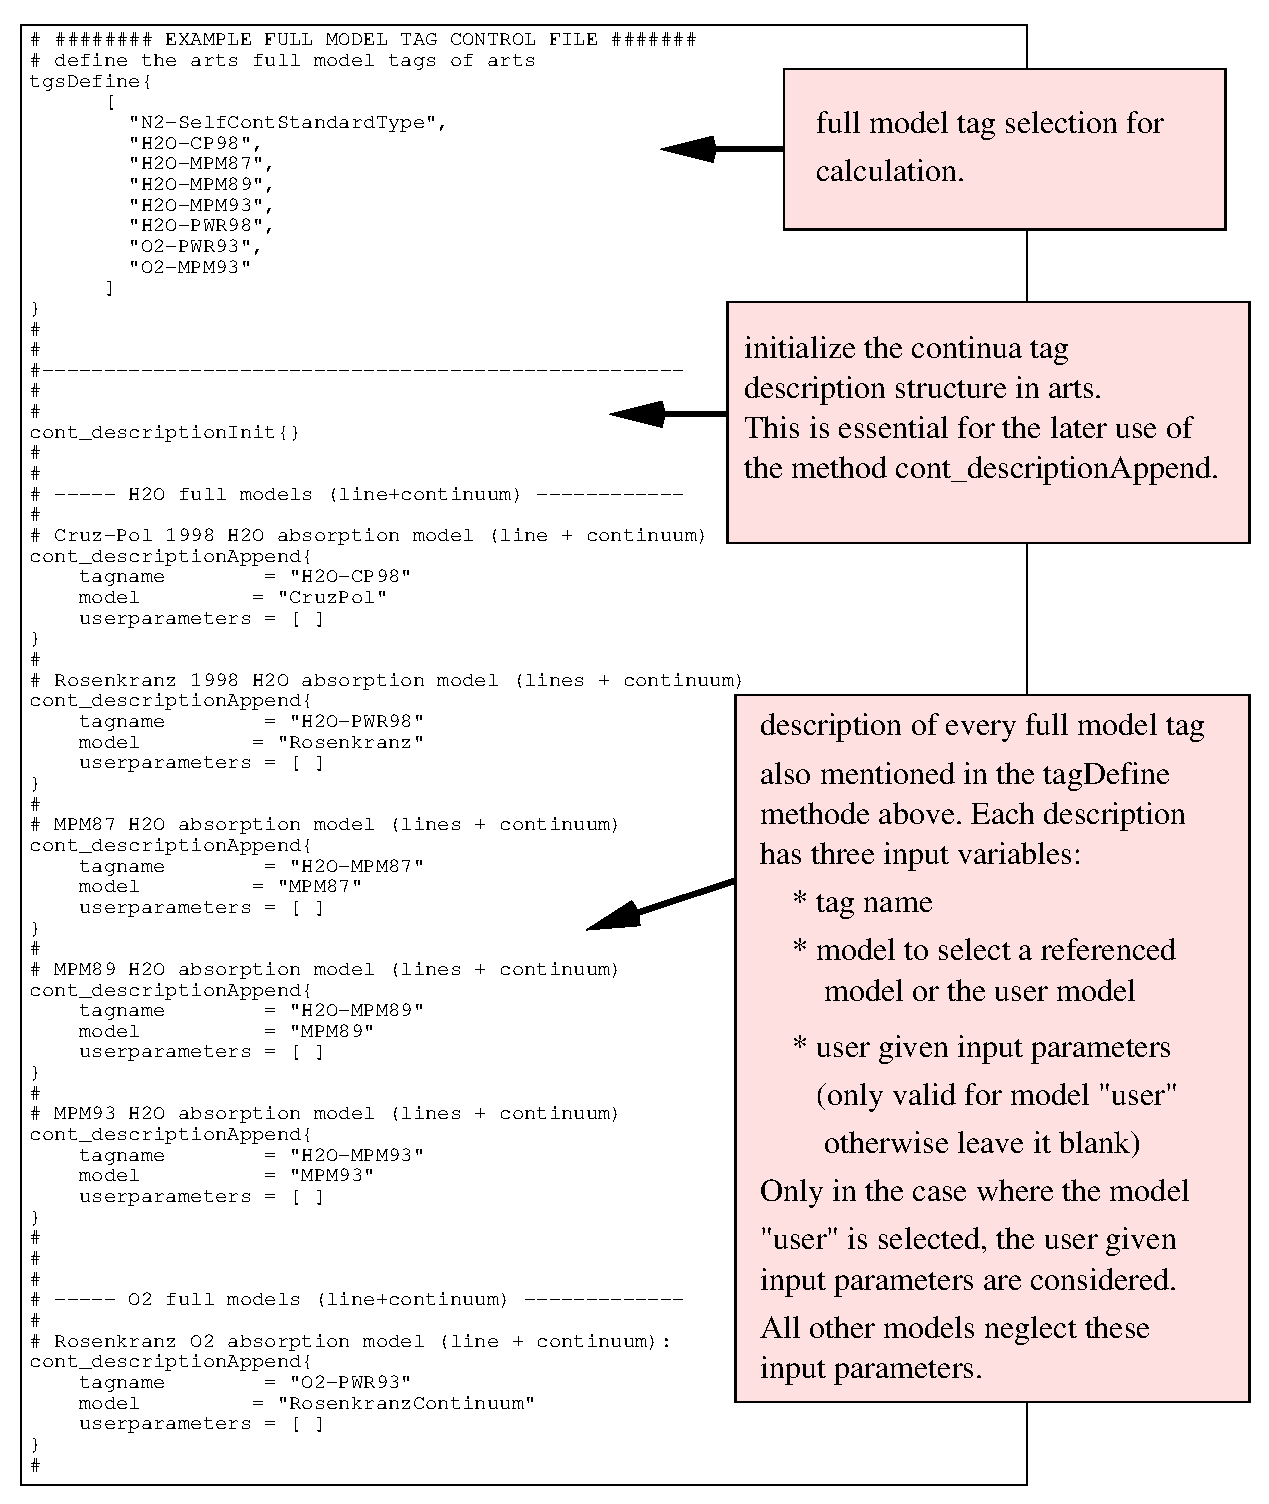
\includegraphics[scale=0.65, angle=0]{fullmodel_description_page1}
\end{flushleft}
\begin{flushleft}
 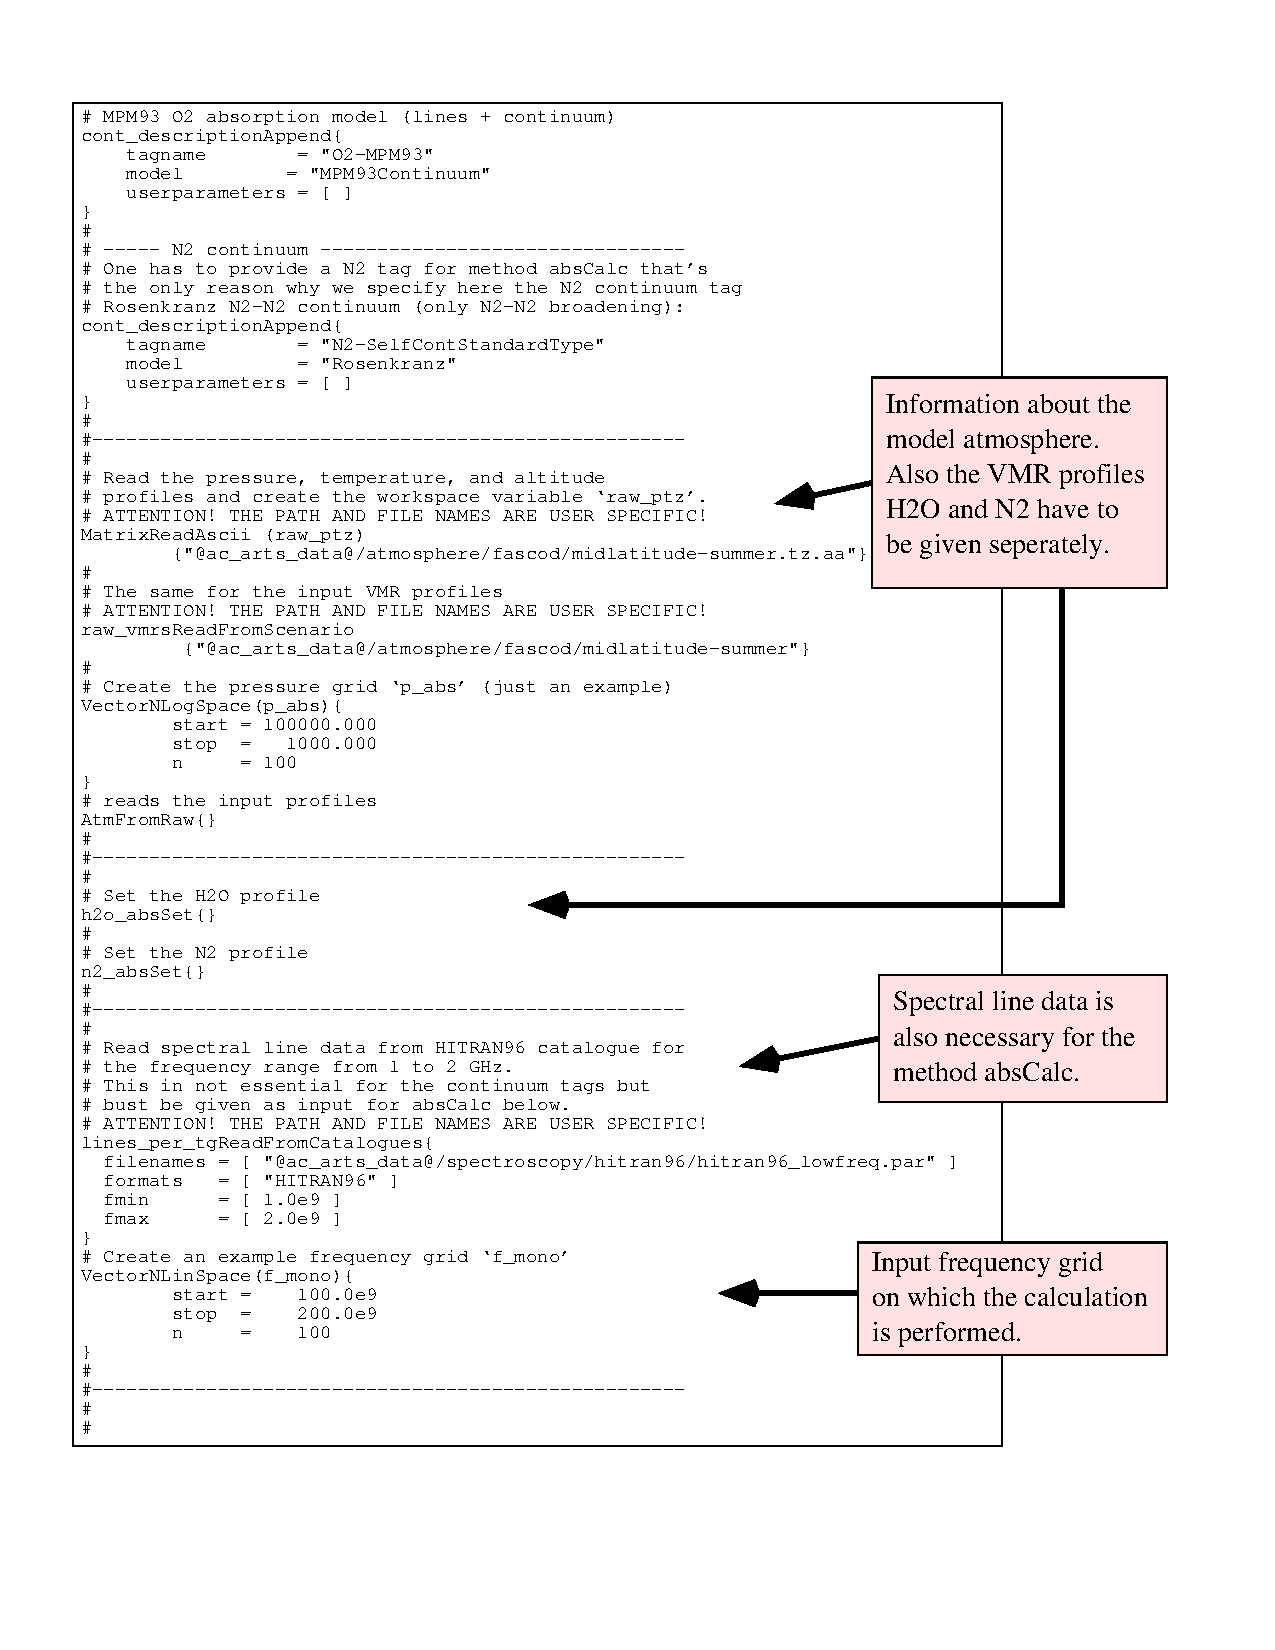
\includegraphics[scale=0.65, angle=0]{fullmodel_description_page2}
\end{flushleft}
\begin{flushleft}
 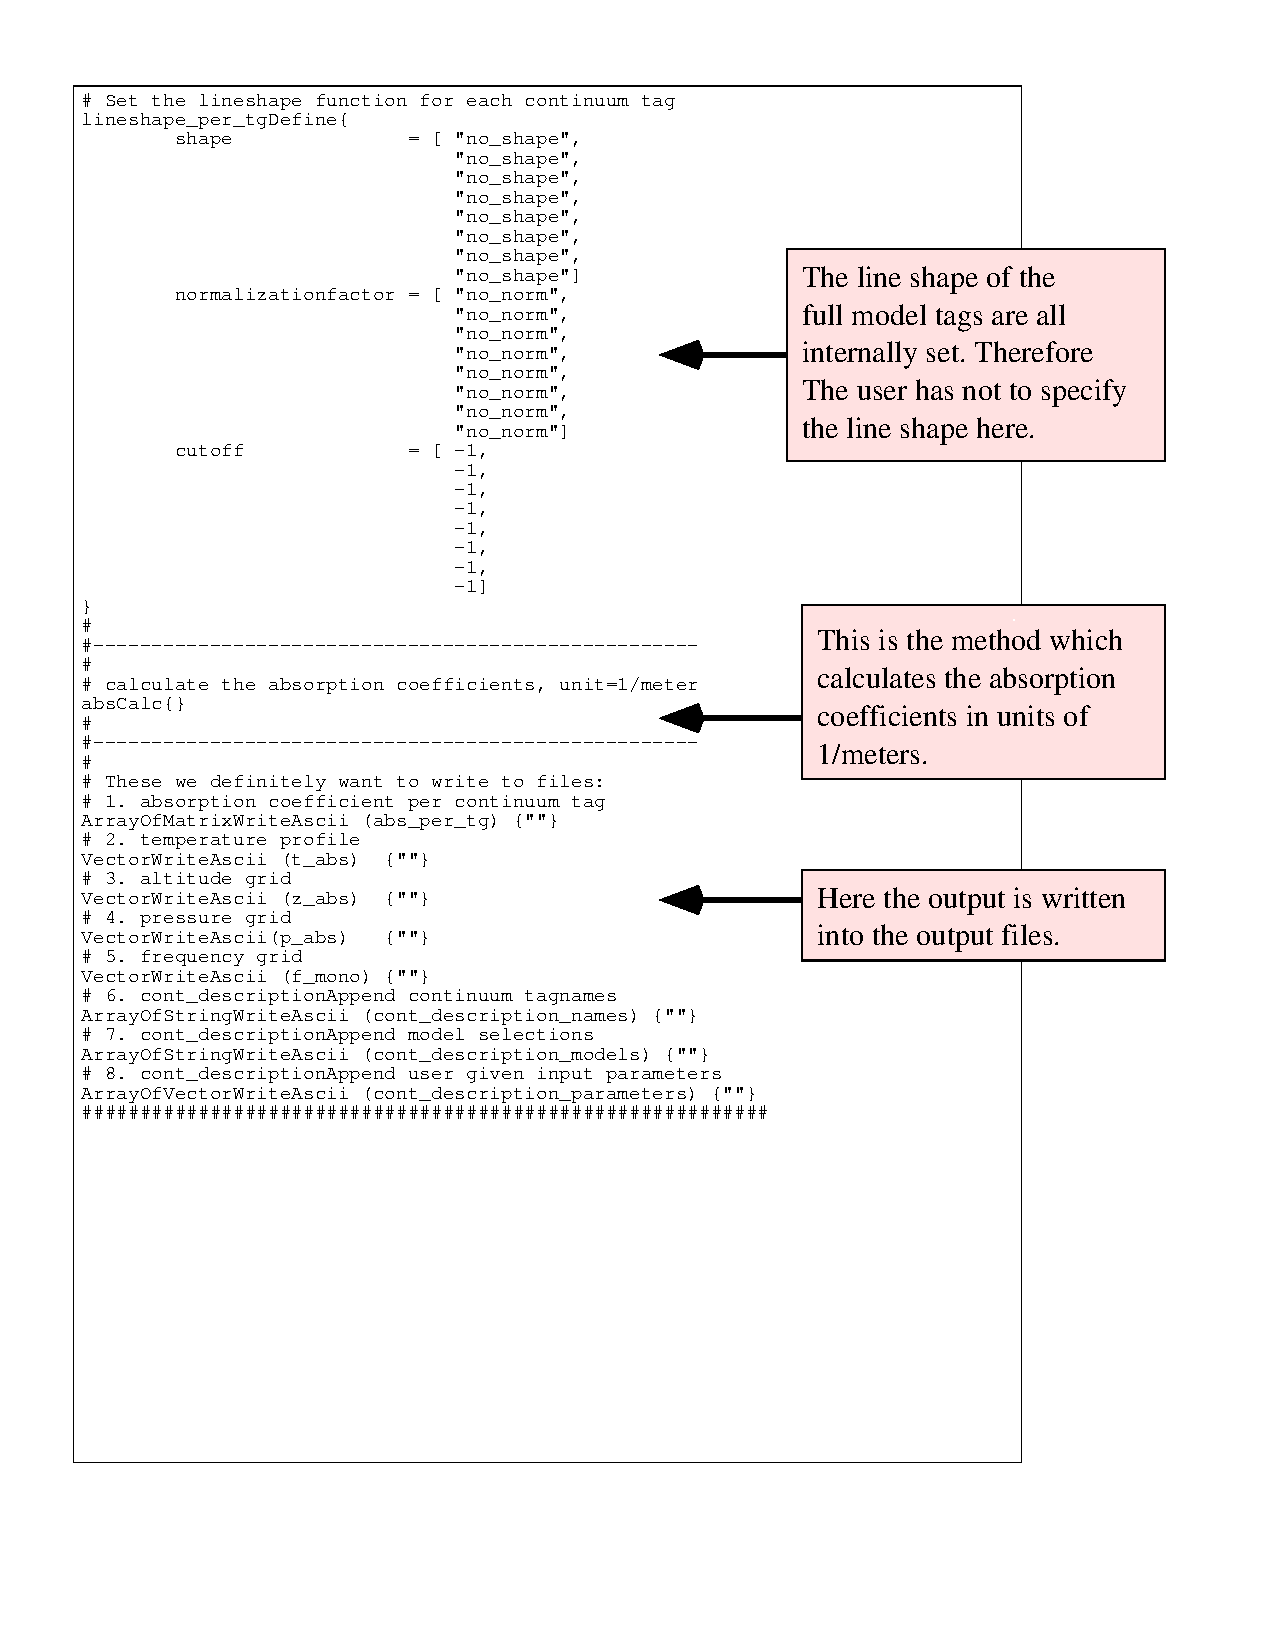
\includegraphics[scale=0.65, angle=0]{fullmodel_description_page3}
\end{flushleft}






%############################################################################# 

% ================================================================================
% The following section is written by Thomas Kuhn, iup Bremen, tkuhn@uni-bremen.de
% ================================================================================

\levela{Cloud Absorption}
\label{labela:cloudabsorption}
%=============================

\levelb{Liquid water and ice particle absorption}
\label{levelb:lipartabs}
%*************************************************
So far only absorption due to air was described. However 
hydrometeors\footnote{We denote liquid water and ice particles, either
  suspended or precipitating, in the air as hydrometeors.}
can have a noticeable effect on the radiative transfer through the
atmosphere in the 10-30\,GHz frequency range.

The MPM93 model provides beside the absorption model of air also an
absorption model for suspended liquid water droplets and ice particles
\citep{liebe:89b,liebeetal:91,hufford:91,liebeetal:93}.  The model is
applicable for the Rayleigh regime, for which the relation $r <
0.05\cdot \lambda$ holds where $r$ is the particle radius and
$\lambda$ is the wavelength\footnote{See \citet{brussaard:95}, page
  81, for details.}, e. g. for a frequency of around 22\,GHz 
this means $r<$~500\,$\mu$m. Considering \citet{salby:96}, this criterium is --
except for cirrus -- nearly for every aerosol and cloud class
satisfied. But one has to bear in mind that these values have a wide
range of variability, for example, \citet{salby:96} states that the
mean particle radius for stratus, cumulus, and nimbus clouds can be in
the range of 10-1000\,$\mu$m and that the particle radius distribution
is highly unsymmetric. 

With respect to the imaginary part of the complex refractivity, a 
unified parameterization of liquid and ice particle absorption 
is formulated in MPM93:
\begin{eqnarray}
  \label{eq:abs_cloud}
  \alpha & = & 0.1820 \cdot \nu \cdot\imn\hspace*{20mm}
               \mbox{dB/km}\\
    \imn & = & \frac{3}{2} \cdot \frac{w}{m} \cdot 
               \Im{[(\er-1)/(\er+2)]}\nonumber\\
    \imn & = & \frac{3}{2} \cdot \frac{w}{m} \cdot 
               \left[\frac{3\cdot\ime}{(\ree+2)^2~+~(\ime)^2}\right]\nonumber\\
  \nonumber
\end{eqnarray}
where $w$ is the liquid water (0.0\,$<LWC<$\,5.0\,g/m$^3$) or ice
mass (0.0\,$IWC$\,1.0\,g/m$^3$) content and $m$ is the water 
or ice bulk density ($\denli$=1.0\,g/cm$^3$ and 0.916\,g/cm$^3$, respectively).\\
The difference between liquid water and ice absorption is put in the 
expressions for the complex permittivities (i. e. the relative 
dielectric constant), $\er=\ree+i\cdot\ime$, which depend on frequency
and temperature.

\noindent$\bullet$ Complex permittivity for suspended liquid water droplets:
\begin{eqnarray}
  \label{eq:comp_perm_lwc}
  \ree       & = & \epsilon_o~-~\nu^2\cdot
                   \left[\frac{\epsilon_o-\epsilon_1}{\nu^2+\gamma_1^2}~+~
                   \frac{\epsilon_1-\epsilon_2}{\nu^2+\gamma_2^2}\right]\nonumber\\
%
  \ime       & = & \nu\cdot\left[\gamma_1\cdot
                   \frac{\epsilon_o-\epsilon_1}{\nu^2+\gamma_1^2}~+~
                   \gamma_2\cdot\frac{\epsilon_1-\epsilon_2}{\nu^2+\gamma_2^2}\right]\nonumber\\
%
  \label{eq:comp_perm_lwc_epsilon_0}
  \epsilon_o & = & 77.66 + 103.3\cdot(\Theta-1)\\
  \epsilon_1 & = & 0.0671\cdot\epsilon_o\nonumber\\
  \epsilon_2 & = & 3.52\nonumber\\
%
  \label{eq:comp_perm_lwc_gamma_1}
  \gamma_1   & = & 20.20 - 146\cdot(\Theta-1) + 316\cdot(\Theta-1)^2\,\mbox{GHz}\\
  \gamma_2   & = & 39.8\cdot\gamma_1\,\mbox{GHz}\nonumber\\
%
  \Theta     & = & 300\,\mbox{K}~/~T\nonumber
%
%  LWC        & = & 0.0~\mbox{to}~5.0~\mbox{g}/\mbox{m}^3
%                   \hspace*{10mm}\mbox{cloud liquid water content}\nonumber\\
%  \rho_l     & = & 1.0~\mbox{g}/\mbox{cm}^3
%                \hspace*{10mm}\mbox{water density}\nonumber
%  \nonumber
\end{eqnarray}
$\bullet$ Complex permittivity for ice crystals:
\begin{eqnarray}
  \label{eq:comp_perm_iwc}
  \ree    & = & 3.15\nonumber\\
%
  \ime    & = & \frac{a}{\nu}~+~b\cdot\nu\nonumber\\
%
  \label{eq:comp_perm_iwc_a}
  a       & = & (\Theta-0.1871)\cdot\exp{(17.0-22.1\cdot\Theta)}\\
  \label{eq:comp_perm_iwc_b}
  b       & = & \left[\left(\frac{0.233}{1-0.993/\Theta}\right)^2 + 
                \frac{6.33}{\Theta} - 1.31\right]\cdot10^{-5}\\
%
  \Theta  & = & 300\,\mbox{K}~/~T\nonumber
%
%  IWC     & = & 0.0~\mbox{to}~1.0~\mbox{g}/\mbox{m}^3 
%                \hspace*{10mm}\mbox{cloud ice water content}\nonumber\\
%  \rho_i    & = & 0.916~\mbox{g}/\mbox{cm}^3
%                \hspace*{10mm}\mbox{ice density}\nonumber
%  \nonumber
\end{eqnarray}
%
The absorption is directly proportional to the liquid or ice water
content $LWC/IWC$ and inversely proportional to the density of a
single liquid ice particle $\denli$. Like the mean particle radius,
the liquid and ice water content have a high variability. Table
\ref{tab:lwc} reflects this variability by summarizing different
literature values for several cloud types. Additional uncertainty 
of this absorption term comes from two sides: 
(1) the difference to the Rayleigh approximation
of the order of 1-6\% as reported in \citet{lietal:97} and (2) from
the fit of the complex permittivity.  Since $\epsilon(\nu,T)$ was
fitted to measurements which were mostly performed above $0^\circ$C,
the extrapolated values for $T<$0$^{\rm o}$C for super-cooled
clouds are not well established. For example in \cite{liebeetal:91} 
itself two different parameterizations for the so called primary 
relaxation frequency ($\gamma_1$ in Equation \ref{eq:comp_perm_lwc}) 
are given, one polynomial in $\Theta$ as presented in 
Equation \ref{eq:comp_perm_lwc}) and an exponential function derived
from theory. Although the polynomial describes the selected 
data better than the exponential function, this might not be true for
temperatures well below 0$^{\rm o}$C.
The difference in $\gamma_1$ according to these two approaches can 
be more than 2\,GHz for very low temperatures \citep{liptonetal:99}. 
The resulting consequences from this discrepancy for the absorption 
calculation at three microwave frequencies are shown in 
Figure \ref{fig:refrac_water_comp}. A more detailed
discussion about this source of uncertainty is given in Section
\ref{levelb:ref_uncert_clouds}.
%
\begin{table}[!htb]
\begin{center}
\begin{tabular}{llll}
\hline
\multicolumn{4}{c}{liquid water content ($LWC$)} \\
 cloud        & class & \multicolumn{1}{c}{(g/m$^3$)} & reference\\
\hline
 stratus      & St    & 0.15        & \cite{salby:96}\\
              &       & 0.09-0.9    & \cite{seinfeld:98}\\
              &       & 0.28-0.3    & \cite{hess:98}\\
              &       & 0.29        & \cite{abreu:96}\\
 nimbostratus & Ns    & 0.4         & \cite{salby:96}\\
              &       & 0.65        & \cite{abreu:96}\\
              &       & 0.05-0.3    & \cite{berton:00}\\
 altostratus  & As    & $<$0.01-0.2 & \cite{seinfeld:98}\\
              &       & 0.41        & \cite{abreu:96}\\
              &       & 0.1-1       & \cite{berton:00}\\
 stratocumulus& Sc    & 0.3         & \cite{salby:96}\\
              &       & $<$0.1-0.7  & \cite{seinfeld:98}\\
              &       & 0.15        & \cite{abreu:96}\\
              &       & $<$0.5      & \cite{pawlowskaetal:00}\\
              &       & 0.05-1      & \cite{berton:00}\\
 cumulus      & Cu    & 0.5         & \cite{salby:96}\\
              &       & 0.26-0.44   & \cite{hess:98}\\
              &       & 1.00        & \cite{abreu:96}\\
 cumulonimbus & Cb    & 2.5         & \cite{salby:96}\\
              &       & 0.1-2       & \cite{berton:00}\\
 cumulus 
    congestus & Cg    & 0.1-3.2     & \cite{berton:00}\\
FIRE-ACE      & -     & $<$0.7      & \cite{shupeetal:00}\\
\hline
\multicolumn{4}{c}{}  \\
\multicolumn{4}{c}{ice water content ($IWC$)}  \\
 cloud        & class & \multicolumn{1}{c}{(g/m$^3$)} & reference\\
\hline
 cirrus       & Ci    & 0.025                         & \cite{salby:96}\\
              &       & 0.00193-0.0260                & \cite{hess:98}\\
              &       & 3.128$\cdot$10$^{-4}$-0.06405 & \cite{abreu:96}\\ 
              &       & 0.15-0.3                      & \cite{larsenetal:98}\\
              &       & $<$0.1                        & \cite{berton:00}\\
cirrostratus  & Cs    & 0.2                           & \cite{salby:96}\\
              &       & 0.05-2                        & \cite{berton:00}\\
\hline
\end{tabular}
\caption{Stated values for the liquid and ice water content of several 
  cloud classes from different sources.}
\label{tab:lwc}
\end{center}
\end{table}



\levelb{Variability and Uncertainty in Cloud Absorption}
\label{levelb:ref_uncert_clouds}
%--------------------------------------------------------
In the case of clouds three sources of uncertainties can be considered
at first sight: (1) validity of the Rayleigh approximation (2) the 
parameterization of the relative dielectric constants ($\er$) of water 
and ice in the microwave region, and (3) the statistical and
climatological variability of the cloud liquid water and ice content.

As it was stated above (Section \ref{levelb:lipartabs}) the Rayleigh 
approximation is valid for particle sizes $<$~500\,$\mu$m. Figure 
\ref{fig:cloud_part_dist} shows a particle size distribution for water
clouds and ice clouds (cirrus) from the OPAC model \citep{hess:98}. 
According to this model only cirrus clouds will have particles of size
larger than 500\,$\mu$m. Nevertheless one has to keep in mind that the
variability of the particle size can be very high so that at certain 
conditions some cloud types (most probable is the cumulonimbus) 
a non-negligible large particle concentration can occur.

The uncertainty in the relative dielectric constant of water 
(see e.~g. \citet{liptonetal:99}) is largest below the freezing 
temperature, since only a few measurements at -4$^{\rm o}$C 
contributed to the parameterization of $\er$ in \cite{liebeetal:91}, 
which in turn is used in the cloud liquid water absorption model of MPM93. 
Figure \ref{fig:refrac_water_comp} shows a comparison of 
\cite{liebeetal:91} and \cite{ray:72}\footnote{{The calculations
  for this parameterizastion are performed with the computer code}\\{
   of W. Wiscombe, NASA, GSFC}\\
  (ftp://climate.gsfc.nasa.gov/pub/wiscombe/Refrac\_Index/WATER/)
  For the microwave frequency range this program uses the
  \cite{ray:72} temperature parameterization.} parameterizations 
for the temperature dependence of the expression
$\Im{[(\er-1)/(\er+2)]}$, which is in the Rayleigh approximation 
one of the relevant terms in the absorption calculation (see 
Equation \ref{eq:abs_cloud}). Additionally the same calculations with 
the alternative expression of the first  relaxation frequency, 
$\gamma_1$, as stated in Equation~2b of \cite{liebeetal:91} is shown. 
The three versions give comparable results for temperatures warmer 
than 260\,K but show significant  differences for temperatures below 
240\,K. However, an uncertainty estimation of $\Im{[(\er-1)/(\er+2)]}$ 
is due to the lack of measurements not easy, but it will certainly
increase with decreasing temperature.

The largest variability of the involved quantities of cloud absorption
is the liquid and ice water content ($LWC$ and $IWC$) of the clouds 
(see Table \ref{tab:lwc}). Even within a single cloud the $LWC$ ($IWC$) changes
with altitude and the distance from the cloud center as can be seen for
example in Figure 10 of \citet{ludlammason:57} and in the model study
of \citet{costaetal:00}.




\levelb{Water Vapor Saturation Adjustment in the Cloud}
\label{levelb:WV_sat_in_cloud}
%--------------------------------------------------------

The arts method {\tt WaterVaporSaturationInClouds{}} assures that 
the water vapor partial pressure is automatically set to 
saturation pressure (100\,\% relative humidity) in the cloud vertical
range.
This method sets the water vapor partial pressure to the 
saturation pressure over liquid water in case where liquid clouds 
are present and to the saturation pressure over ice where 
ice or water/ice clouds are present. The calculation of the 
saturation pressure is calculated according to the 
Goff-Gratch approximation \citep{liebeetal:93}:

\begin{eqnarray}
  \theta &=& (373.16\,\mbox{K} / T) \\
%
  x      &=& A \cdot \left(\theta -1 \right) + 
             B \cdot \log{(\theta)} + \nonumber\\ 
         &&  C \cdot \left( 10^{d\cdot (1- \theta^{-1})} -1 \right) +  
             E \cdot \left( 10^{g\cdot (\theta-1)} -1 \right) \\ 
%
  e^w_s  &=& 101324.6 \cdot 10.0^x\,\mbox{Pa} 
\end{eqnarray}
with
\begin{eqnarray}
 A &=& -7.90298 \nonumber \\
 B &=& 5.02808  \nonumber \\
 C &=& -1.3816 \cdot 10^{-7} \nonumber \\
 d &=& 11.344 \nonumber \\
 E &=& 8.1328 \cdot 10^{-3} \nonumber \\
 g &=& -3.49149 \nonumber
\end{eqnarray}


The $\hzo$ saturation pressure over ice the Goff-Gratch 
approximation \citep{liebeetal:93} is as follows:
\begin{eqnarray}
  \theta &=& (273.16\,\mbox{K} / T) \\
%
  x      &=& A \cdot \left(\theta -1 \right) + 
             B \cdot \log{(\theta)} + 
             C \cdot \left( 1- \theta^{-1} \right) \\ 
%
  e^i_s  &=& 610.71 \cdot 10.0^x\,\mbox{Pa} 
\end{eqnarray}
with
\begin{eqnarray}
 A &=& -9.09718  \nonumber \\
 B &=& -3.56654  \nonumber \\
 C &=&  0.876793 \nonumber
\end{eqnarray}



\begin{figure}[!htb]
  \begin{center}
% ---- uncertainty -------------------------------------
%   \includegraphics*[scale=0.6, angle=90, viewport= 80 725 480 70]%
   \includegraphics*[width=0.6\hsize, angle=90]%
   {LWCcloud}\\
% ---- ratio -------------------------------------------
%   \includegraphics*[scale=0.6, angle=90, viewport= 80 725 480 66]%
   \includegraphics*[width=0.6\hsize, angle=90]%
   {IWCcloud}
% ------------------------------------------------------
  \end{center}
  \caption{Cloud particle size distributions according to 
    Equations~3a and 3c and the microphysical properties are from the 
    Tables 1a and 1b of the OPAC model \cite{hess:98}. 
    For the liquid water clouds (upper plot) a modified gamma 
    distribution is assumed whereas for the ice clouds (lower plot) 
    exponential functions are taken.}
  \label{fig:cloud_part_dist}
\end{figure}
%
%
\begin{figure}[!hbt]
  \begin{center}
% ---- comparison --------------------------------------
   \includegraphics*[width=0.75\hsize, angle=0]%
   {refractive_water_comp_T}
% ------------------------------------------------------
  \end{center}
  \caption{Comparison of the imaginary part of the expression 
    \mbox{$(\er-1)/(\er+2)$} for liquid water at the three 
    frequencies of 32.9, 22.6, and 10,3 GHz. Plotted are the two common
    models of \cite{liebeetal:91} (a) and \cite{ray:72} (b). 
    The Ray parameterization is calculated with the F77 program 
    of W. Wiscombe, NASA, GSFC, take from 
    ftp://climate.gsfc.nasa.gov/pub/wiscombe/Refrac\_Index/WATER/.
    Additionally the \cite{liebeetal:91} parameterization (c) with the 
    alternative expression for the first relaxation frequency, 
    $\gamma_1 = 20.1\cdot\exp{[7.88\cdot(1-\Theta)]}$, is plotted.}
%
%    $(\er-1)/(\er+2)$ for liquid water at the three WATS frequencies
%    of interest. Plotted are the two common
%    models of \cite{liebeetal:91} and \cite{ray:72} (calculated with 
%    the F77 program of W. Wiscombe (NASA, GSFC) take from 
%    ftp://climate.gsfc.nasa.gov/pub/wiscombe/Refrac\_Index/WATER/).}
  \label{fig:refrac_water_comp}
\end{figure}




\levelb{ARTS Workspace Variables and Methods}
\label{levelb:ArtsImplementationCloudAbsorption}
% ----------------------------------------------

This section explains how the above described cloud absorption models
are represented in the structure of the arts source code and how 
one can invoke them in the arts control file.

The cloud tags needs not necessarily more input information than 
normal trace gas tags, since both need only a profile. But to have 
more flexibility one can run these absorption models as black boxes 
or with some user given input. In connection with this input parameters 
we distinguish generally two types, the referenced models which 
are taken from the literature (e. g. \cite{liebeetal:93}) and the 
user model, for which the arts user is providing the necessary 
parameter values.

Formally the cloud tags are like the 
continuum or full model tags implemented. Therefore after selecting 
the cloud tag with the {\tt tagDefine} method, the arts user has to 
setup the arts internal structure (i. e. the workspace variables 
{\it cont\_description\_names, cont\_description\_models, 
and cont\_description\_parameters}) for the selected continuum tags, 
which can simply be done by putting the following line into the 
arts control file:
\begin{verbatim}
cont_descriptionInit{}
\end{verbatim}

After this initialization, the cloud tag specific
information has to be transfered to arts. This is possible with the 
arts method {\it cont\_descriptionAppend}, which has itself 
three input variables: {\it tagname}, {\it model}, and 
{\it userparameters}. The user has to specify these input 
variables in the arts control file for each selected cloud tag. 
Below is a list of all the implemented continuum tags and the associated
valid range of the input variables for {\it cont\_descriptionAppend}. 
For an overview of the possible continuum tags and their 
referenced models see Table \ref{tab:artscloudlist} and the 
online documentation can be found under 
{\it arts/doc/doxygen/html/continua\_cc.html}.

One has to note at this place that the two input variables {\it model} and
{\it userparameters} are to some extend redundant. Therefore one can also 
produce an ambiguity by giving contradicting values for these two input variables.
To avoid such ambiguities the arts user should keep in mind the general 
rule that only the user model ({\it model ="user"}) needs input parameters 
via the input variable {\it userparameters}. The referenced models 
need no input via {\it userparameters}. If you try to run the arts control 
file with a referenced model and input parameters you will get an error message.
Below in the detailed description of {\it cont\_descriptionAppend} you 
can find correct examples for all the cloud tags.

\begin{itemize}
\item[$\bullet$] The liquid water cloud absorption model of 
     MPM93 \citep{liebeetal:93} has the arts tag name 
     {\tt "liquidcloud-MPM93"}. The details about this 
     absorption model are described in Section 
     \ref{labela:cloudabsorption}. The standard way to use 
     the MPM93 liquid water cloud absorption model is to set 
     the input variable {\it model} to "MPM93" and leaving 
     the input parameter {\it userparameters} empty. \\ To 
     have a minimum possibility of variation one can also run 
     this tag with {\it model}\,=\,"user". In this case one 
     has to provide three input parameters via {\it userparameters}, 
     e. g. {\it userparameters}\,=\,$[CC$, $CG$, $CE]$. The first 
     input parameter ($CC$) scales the total liquid water cloud absorption 
     (see Eq. \ref{eq:abs_cloud}) while $CG$ scales the first 
     relaxation frequency, $\gamma_1$, (see Eq. 
     (\ref{eq:comp_perm_lwc_gamma_1})) and  $CE$ scales $\epsilon_o$ 
     (see Eq. \ref{eq:comp_perm_lwc_epsilon_0})
\begin{verbatim}
cont_descriptionAppend{
    tagname        = "liquidcloud-MPM93"
    model          = "MPM93"
    userparameters = [ ]
}
cont_descriptionAppend{
    tagname        = "liquidcloud-MPM93"
    model          = "user"
    userparameters = [ 1.0, 1.0, 1.0 ]
}
\end{verbatim}
\item[$\bullet$] The ice water cloud absorption model of 
     MPM93 \citep{liebeetal:93} has the arts tag name 
     {\tt "icecloud-MPM93"}. The details about this 
     absorption model are described in Section 
     \ref{labela:cloudabsorption}. The standard way to use 
     the MPM93 ice water cloud absorption model is to set 
     the input variable {\it model} to "MPM93" and leaving 
     the input parameter {\it userparameters} empty. \\ To 
     have a minimum possibility of variation one can also run 
     this tag with {\it model}\,=\,"user". In this case one 
     has to provide three input parameters via {\it userparameters}, 
     e. g. {\it userparameters}\,=\,$[CC$, $CA$, $CB]$. The first 
     input parameter ($CC$) scales the total ice water cloud absorption 
     (see Eq. \ref{eq:abs_cloud}) while $CA$ scales $a$, (see Eq. 
     (\ref{eq:comp_perm_iwc_a})) and $CB$ scales $b$ 
     (see Eq. \ref{eq:comp_perm_iwc_b})
\begin{verbatim}
# MPM93 model for ice water particle absorption:
cont_descriptionAppend{
    tagname        = "icecloud-MPM93"
    model          = "MPM93"
    userparameters = [ ]
}
# MPM93 model for ice water particle absorption:
cont_descriptionAppend{
    tagname        = "icecloud-MPM93"
    model          = "user"
    userparameters = [ 1.0, 1.0, 1.0 ]
}
\end{verbatim}
\end{itemize}


Another important point is to state in the arts control file which
cloud profile should be read in. Becasue for a single climate zone one
can have several different cloud types, it is not enough to state 
e. g. just {\it midlatitude-summer} or {\it tropical} as for 
trace gases. Therefore the method {\tt raw\_vmrsReadFromFiles} has to 
be used to read in the trace gas and clooud profiles. For example 
the following lines in the control file will read in trace gas 
profiles from a midlatitude-summer scenario (this information is
provided with the input variable {\it basename} which states the 
basic scenario) and cumulonimbus and cirrus cloud profiles for 
liquid water and ice water clouds, respectively:
\begin{verbatim}
# ATTENTION! THE PATH AND FILE NAMES ARE USER SPECIFIC!
raw_vmrsReadFromFiles
  {seltags   = [ "liquidcloud-MPM93", 
                 "icecloud-MPM93" ]
   filenames = [ "cumulonimbus.MPM93droplet.aa",
                 "cirrus.MPM93ice.aa" ]
   basename  =   "midlatitude-summer"
  }
#
\end{verbatim}
The method {\tt raw\_vmrsReadFromFiles}can be used for any tag and 
is not specific for cloud tags. In general one has to state in the 
input variable {\it seltags} the tags which take their profile 
information from the files stated in the input variable 
{\it filenames}, while all the tags which are not stated in 
{\it seltags} take their profile information, i. e. the atmospheric 
scenario, from the input variable {\it basename}. 

To set the water vapor pressure in the cloud range to the saturation 
pressure you can use the method {\tt WaterVaporSaturationInClouds{}}
after the call of the method {\tt AtmFromRaw{}}. The saturation
pressure is calculated over liquid water in liquid water clouds and
over ice in ice water clouds. If both cloud types are present the
saturation over ice is taken.

\begin{landscape}
 \setlength{\LTcapwidth}{180mm} % with of the caption in longtable
 \begin{longtable}{llllll}
 K & K & K & K & K & K \kill
%
% --------------------- only begin of table ------------------------------
 \hline
 continuum & \multicolumn{3}{c}{{\it cont\_descriptionAppend} input} & 
 reference/ & arts source code function\\
 & \multicolumn{3}{c}{input parameter} & arts uguide & \\
 \hline
 \endfirsthead
% --------------------- every page begin of table ------------------------
 \hline
 continuum & \multicolumn{3}{c}{{\it cont\_descriptionAppend}} & 
 reference/ & arts source code function\\
 & \multicolumn{3}{c}{input parameter} & arts uguide & \\
 \hline
 \endhead
% --------------------- every page end of table ------------------------
 K & K & K & K & K & K \kill
 \hline
 \caption[]{(continued)}\\
 \endfoot
% --------------------- only end of table ------------------------------
 K & K & K & K & K & K \kill 
 \hline
 \caption{This table gives an overview of the implemented referenced 
   cloud absorption models and how they are specified 
   in the arts method {\it cont\_descriptionAppend}. Additionally the 
   reference and the arts source code function names (see file 
   {\it arts/src/continua.cc} are provided. The detailed online 
   documentation can be found under 
   {\it arts/doc/doxygen/html/continua\_cc.html}).}
 \label{tab:artscloudlist}
 \endlastfoot
% --------------------- body of table  ----------------------------------  
 \multicolumn{6}{c}{{\bf water vapor ($\hzo$)}}\\
 \hline
% --------------------------------------------------------------
 MPM93       & tagname &=& {\tt "liquidcloud-MPM93"} & \cite{liebeetal:93} & 
             MPM93WaterDropletAbs\\
             & model   &=& "MPM93"    &   &  \\ 
             & userparameters &=& [ ] &   & \\
 \hline
% --------------------------------------------------------------
 MPM93       & tagname &=& {\tt "icecloud-MPM93"} & \cite{liebeetal:93} & 
               MPM93IceCrystalAbs\\
             & model   &=& "MPM93"    &   &  \\ 
             & userparameters &=& [ ] &   & \\
 \hline
% -----------------------------------------------------------------------  
 \end{longtable}
 \setlength{\LTcapwidth}{0.8\textwidth}
\end{landscape}




\leveld{ARTS Example Control File for the Full Model Tags}
\label{leveld:ArtsCloudModelExampleControlFile}
% --------------------------------------------------------
Below you will find an example of a control file for all 
the implemented cloud absorption models. At the moment only 
the MPM93 model for water and ice clouds is implemented.
Please note that to run this example control file you 
have to specify user specific paths and input file names 
to run it properly. You can find this example in the 
arts directory {\it arts/doc/examples/cloud\_example.arts}
%
\begin{flushleft}
 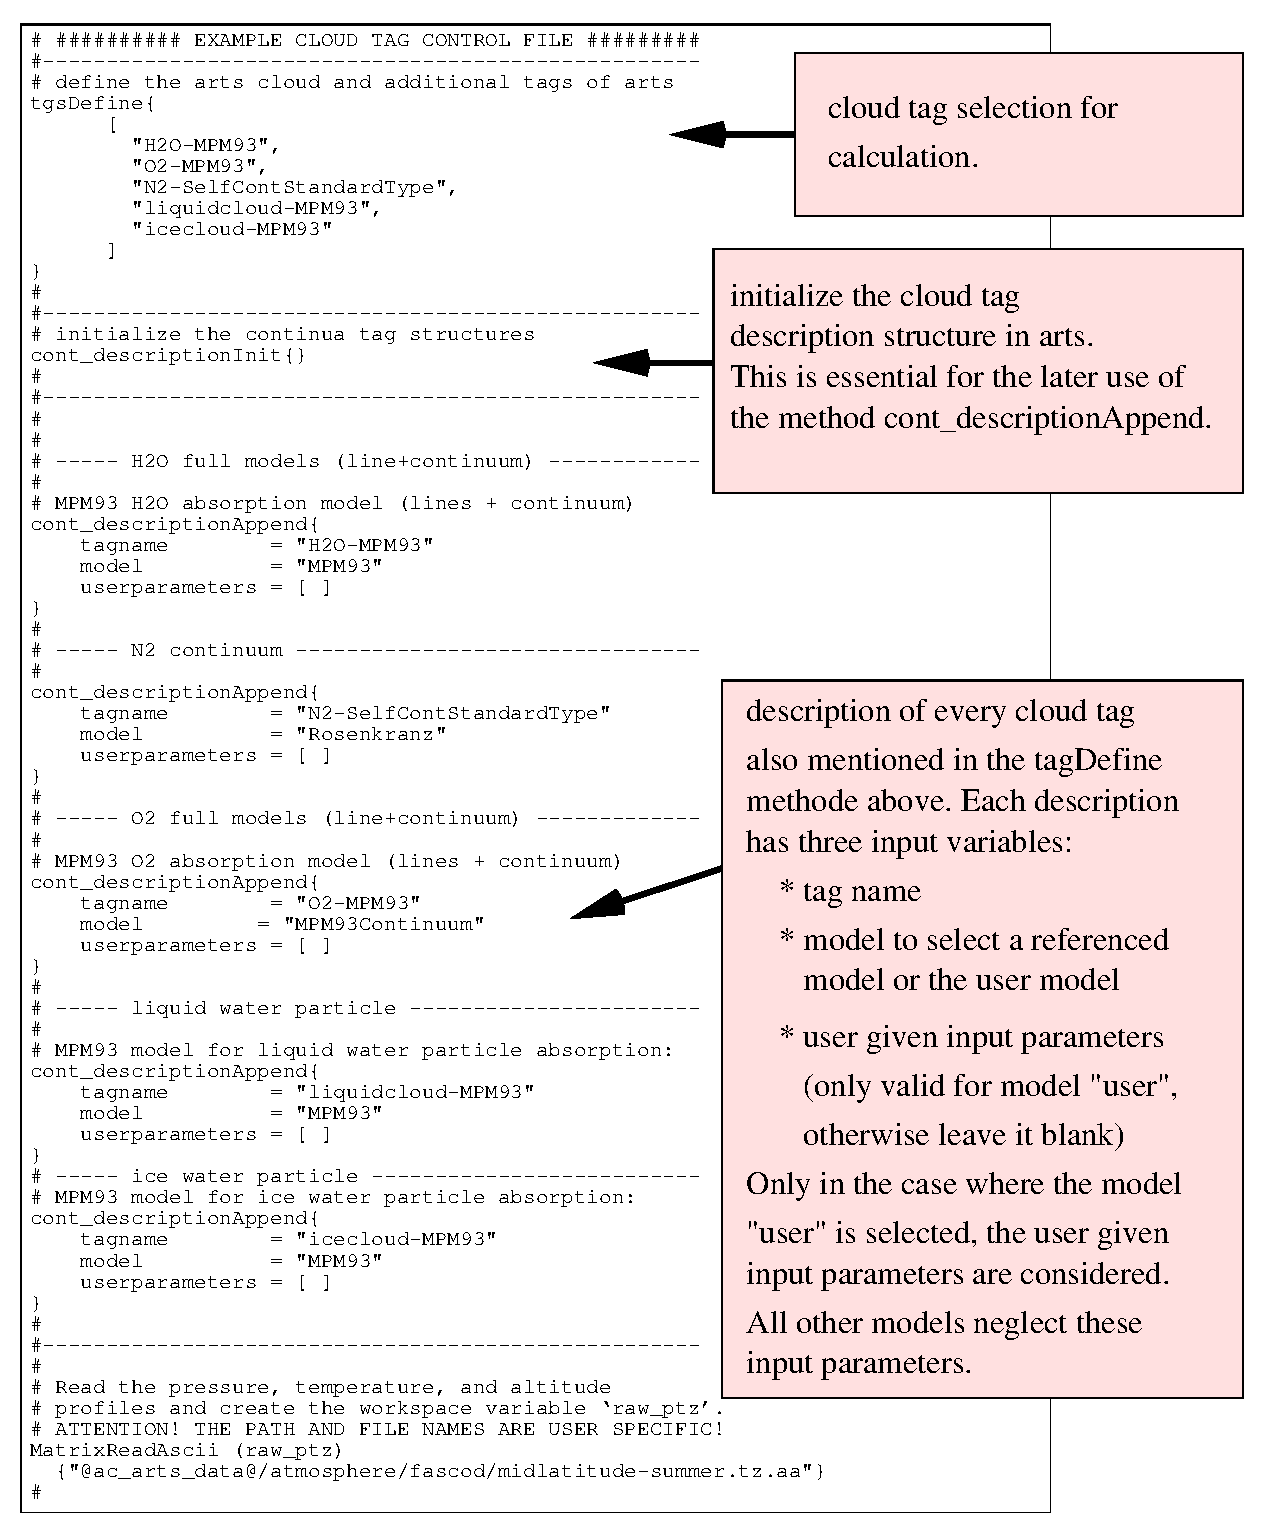
\includegraphics[scale=0.65, angle=0]{cloud_description_page1}
\end{flushleft}
\begin{flushleft}
 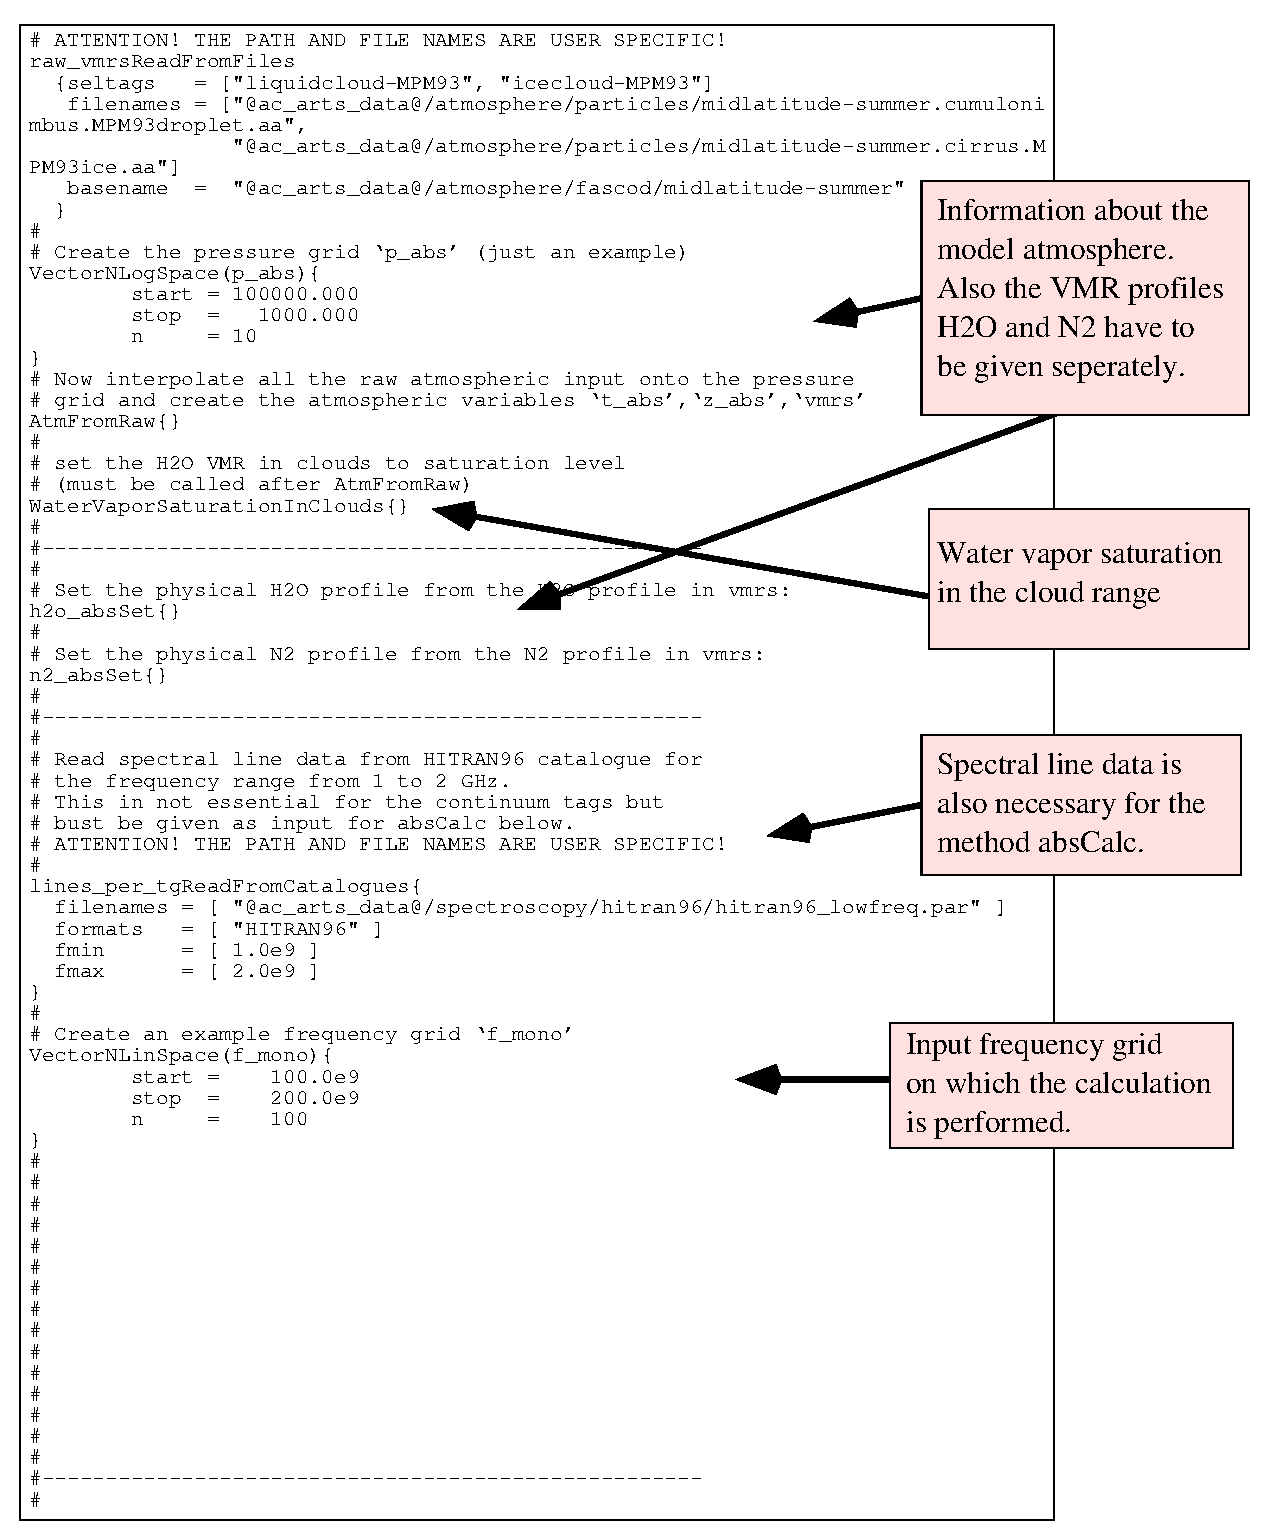
\includegraphics[scale=0.65, angle=0]{cloud_description_page2}
\end{flushleft}
\begin{flushleft}
 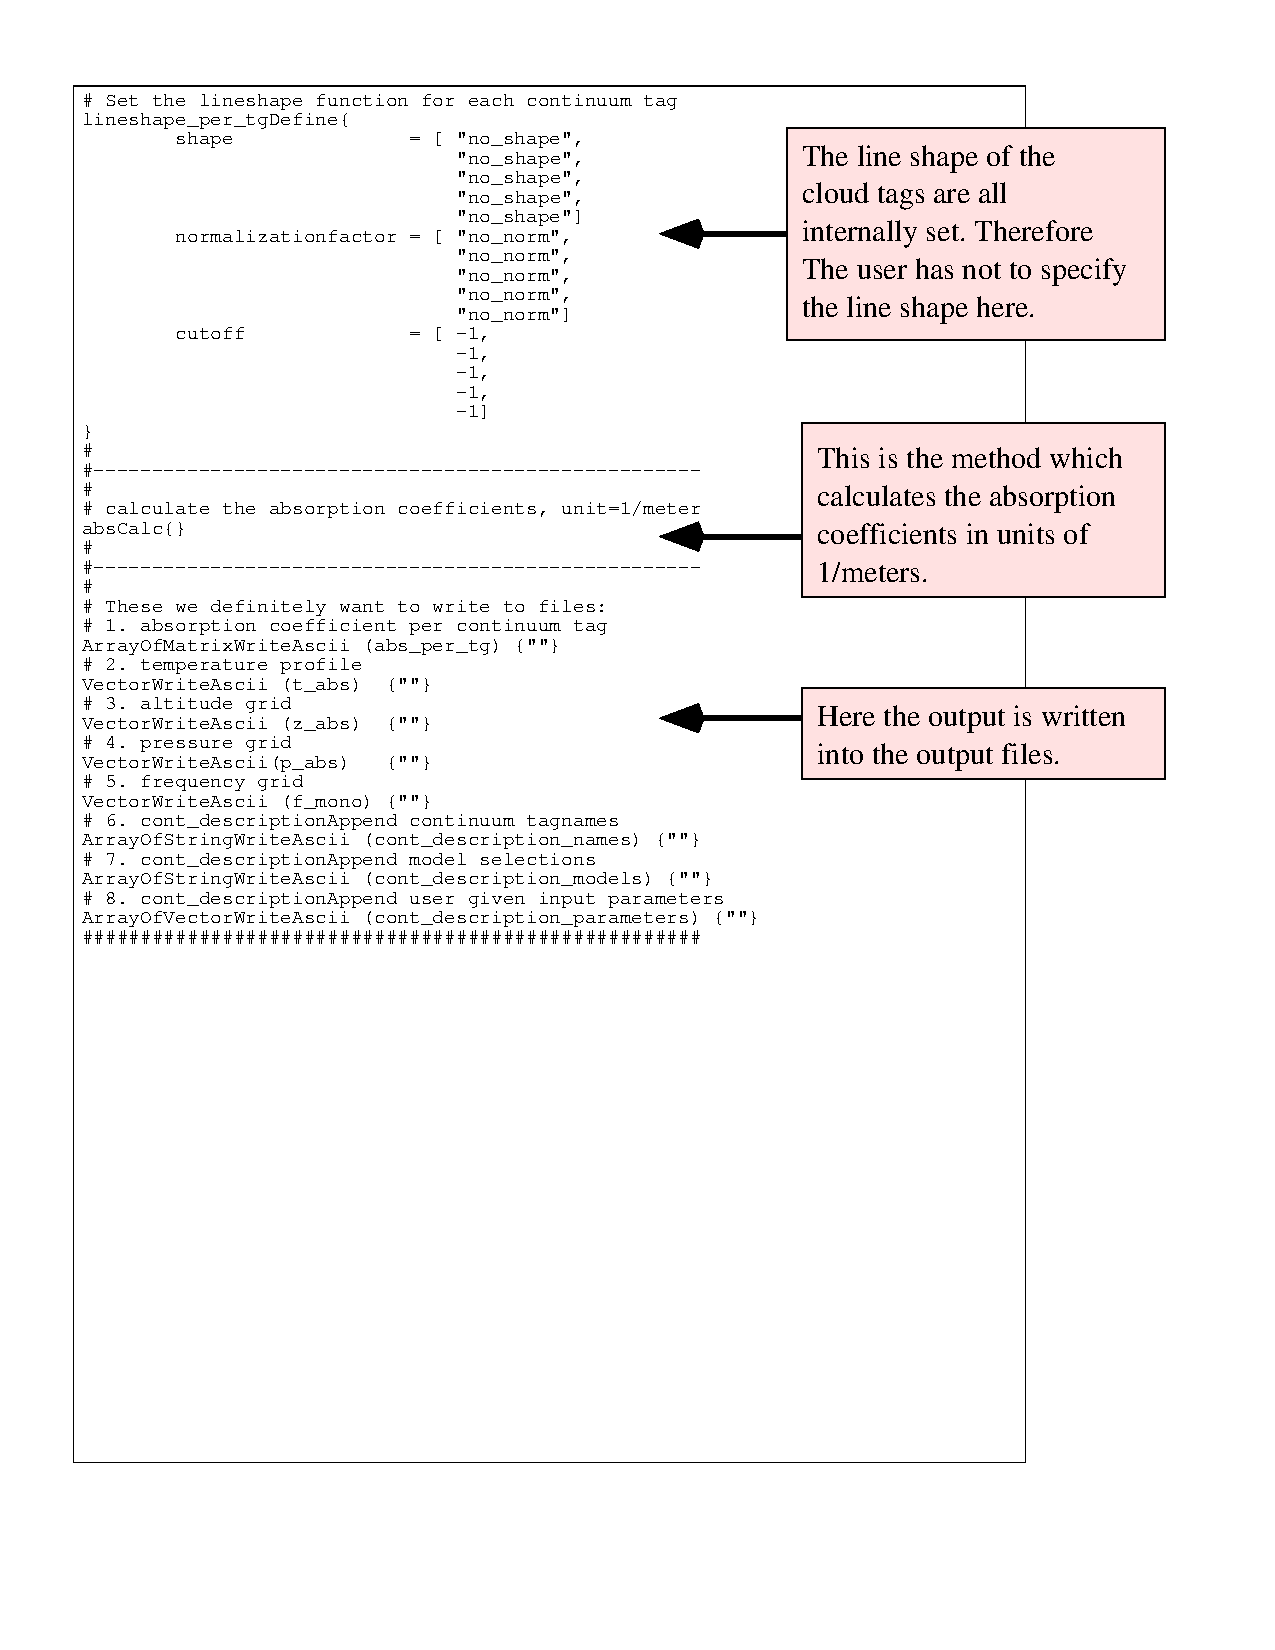
\includegraphics[scale=0.65, angle=0]{cloud_description_page3}
\end{flushleft}



%%% Local Variables: 
%%% mode: latex 
%%% TeX-master: "uguide"
%%% End:

% LocalWords:  Atmosperic

\include{refr_index}
\graphicspath{{Figs/clouds/}}

\chapter{Description of clouds}
 \label{sec:clouds}

\starthistory
 050913 & Created and written by Claudia Emde\\ 
\stophistory

\section{Introduction}
\label{sec:clouds:intro}

In the Earth's atmosphere we find liquid water clouds consisting of
approximately spherical water droplets and cirrus clouds consisting of
ice particles of diverse shapes and sizes. We also find different
kinds of aerosols. In order to take into account this variety, the
model allows to define several \emph{particle types}. A particle type
is either a specified particle or a specified particle distribution,
for example a particle ensemble following a gamma size distribution.
The particles can be completely randomly oriented, azimuthally
randomly oriented or arbitrarily oriented. For each particle type
being a part of the modeled cloud field, a data file containing the
single scattering properties ($\langle\ExtMat_i\rangle$,
$\langle\AbsVec_i\rangle$, and $\langle\PhaMat_i\rangle$), and the
appropriate particle number density field is required. The particle
number density fields are stored as \typeindex{GField3}, including the
field stored in a three-dimensional tensor and also the appropriate
atmospheric grids (pressure, latitude and longitude grid). For each
grid point in the cloud box the single scattering properties are
averaged using the particle number density fields.  In the scattering
database the single scattering properties are not always stored in the
same coordinate system. For instance for randomly oriented particles
it makes sense to store the single scattering properties in the
so-called scattering frame in order to reduce memory requirements. 
The following section describes in detail the \typeindex{SingleScatteringData}
class.  The consequent section describes how to realize different
kinds of size distributions in the ARTS frame by defining appropriate
particle number density fields. 


\section{\textindex{Single scattering properties}}
\label{sec:clouds:ssp}

\subsection[Coordinate systems]{\textindex{Coordinate systems}: The
  \textindex{laboratory frame} and the \textindex{scattering frame} }
\label{sec:clouds:coordinate_sytems}

For radiative transfer calculations we need a coordinate system to
describe the direction of propagation. For this purpose we use the
laboratory frame, which is also shown in
\theory, Figure \ref{T-fig:RT_theory_coordinates}.  The z-axis corresponds to the
local zenith direction and the x-axis points towards the
north-pole. The propagation direction is described by the local zenith
angle $\theta$ and the local azimuth angle $\phi$.  This coordinate
system is the most appropriate frame to describe the propagation
direction and the polarization state of the radiation.  However, in
order to describe scattering of radiation by a particle or a particle
ensemble, it makes sense to define another coordinate system taking
into consideration the symmetries of the particle or the scattering
medium, as one gets much simpler expressions for the single scattering
properties.  For macroscopically isotropic and mirror-symmetric
scattering media it is convenient to use the scattering frame, in
which the incidence direction is parallel to the z-axis and the x-axis
coincides with the scattering plane, that is, the plane through the
unit vectors \VctStl{\hat{n}^{\inc}}\ and \VctStl{\hat{n}^{\sca}}. The
scattering frame is illustrated in
Figure \ref{fig:scattering:part_frame}. For symmetry reasons the single
scattering properties defined with respect to the scattering frame can
only depend on the scattering angle $\Theta$,
\begin{equation}
  \label{eq:scat_angle}
  \Theta=\arccos(\hat{\PDir}^{\inc} \cdot {\hat{\PDir}^{\sca}}),
\end{equation}
between the incident and the scattering direction.

\begin{figure}[htbp]
 \begin{center}
   \includegraphics*[width=0.4\hsize]{part_frame}
   \caption{Illustration of the scattering frame. The z-axis coincides with the incident direction $\hat{\PDir}^{\inc}$. The scattering angle $\Theta$ is the angle between  $\hat{\PDir}^{\inc}$ and $\hat{\PDir}^{\sca}$.}
   \label{fig:scattering:part_frame}  
 \end{center}
\end{figure}

\subsection{Scattering datafile structure}
\label{sec:clouds:ARTS_SSP_structure}
 
The single scattering properties are pre-calculated, for example by
using the T-matrix 
code by \citet{Mishchenko:02}, and stored in data-files. Different
methods for the calculation of single scattering properties are
reviewed in \citet{emde05:_phdthesis}. 

The format of the scattering database allows space reduction due to
symmetry for certain special cases, e.g. random orientation or
horizontal alignment. The file format is XML. The data is stored in a
class called \typeindex{SingleScatteringData}, which resides in
the files \fileindex{optproperties.h}. The class consists of the
following 
fields (compare also Table \ref{tab:scattering:datastructure}):

\begin{itemize}
\item  {\sl enum} \shortcode{ptype}: An attribute which contains
  information about the 
  data type, which is the classification of the kind of hydrometeor
  species (randomly oriented, general case~...). This attribute is
  needed in the radiative transfer function to be able to extract
  the physical phase matrix, the physical extinction matrix and the
  physical absorption vector from the data. 
  
  Possible values of ptype are:
  
  \shortcode{PARTICLE\_TYPE\_GENERAL} = 10 \\
  \shortcode{PARTICLE\_TYPE\_MACROS\_ISO} = 20\\
  \shortcode{PARTICLE\_TYPE\_HORIZ\_AL} = 30\\
  
  A more detailed description of the different cases is given below.

\item {\sl String} \shortcode{description}: Here the particle type
  should be specified 
  explicitly. We can have the case randomly oriented particles, but
  furthermore we also have to specify the exact particle properties
  (i.e. size and shape distribution). This can be a longer text
  describing how the scattering properties were generated. It should
  be formatted for direct printout to screen or file.
  
\item {\sl Vector} \shortcode{f\_grid}: Frequency grid [Unit: Hz].
  
\item {\sl Vector} \shortcode{T\_grid}: Temperature grid [Unit: K].
  
\item {\sl Vector} \shortcode{za\_grid}:
  \begin{enumerate}
  \item \shortcode{p10, p30}: Zenith angle grid (Range: 0.0\degree $\le$ za $\le$ 180.0\degree).
  \item \shortcode{p20}: Scattering angle grid (Range: 0.0\degree $\le$ za $\le$ 180.0\degree).
  \end{enumerate}
  
\item {\sl Vector} \shortcode{aa\_grid}: Azimuth angle grid.
  \begin{enumerate}
  \item \shortcode{p10}: Range: -180.0\degree $\le$ aa $\le$ 180.0\degree
  \item \shortcode{p20}: Not needed, since optical properties depend only on
    scattering angle (dummy grid).
  \item \shortcode{p30}: Only half of the grid is required (Range: 0.0\degree $\le$ aa $\le$ 180.0\degree)
  \end{enumerate}
  
  The angular grids have to satisfy the following conditions:
  \begin{itemize}
  \item They have to be equidistant.
  \item The value of the data must be the same for the first and the
    last grid-point. This condition is required for the integration
    routine.
  \item If we only have to store a part of the grid, for example
    \shortcode{za\_grid} only from 0\degree to 90\degree, these two values (0\degree, 90\degree) must be
    grid-points. 
  \end{itemize}
  
\item {\sl Tensor7} \shortcode{pha\_mat\_data}: Phase matrix data
  \EnsAvr\PhaMat\ [Unit: m$^2$]. The dimensions of the data array are:  
  
  \shortcode{[frequency temperature za\_sca aa\_sca za\_inc aa\_inc matrix\_element]}
  
  The order of matrix elements depends on the chosen case. For most
  cases we do not need all matrix elements (see description of cases
  below).

\item {\sl Tensor5} \shortcode{ext\_mat\_data}: Extinction matrix data
  \EnsAvr\ExtMat\ [Unit: m$^2$]. The dimensions are: 

  \shortcode{[frequency temperature za\_inc aa\_inc matrix\_element]}
  
  Again, the order of matrix elements depends on the chosen case.

\item {\sl Tensor5} \shortcode{abs\_vec\_data}: Absorption vector data
  \EnsAvr\AbsVec\ [Unit: m$^2$]. 
  
  The absorption vector is also precalculated. It could be calculated
  from extinction matrix and phase matrix. But this calculation takes
  long computation time, as it requires an angular integration over
  the phase matrix. For the cases with symmetries (e.g., random
  orientation) the data files will not become too large even if we
  store additionally the absorption vector. The dimensions are: 
  
 \shortcode{[frequency temperature za\_inc aa\_inc vector\_element]}
\end{itemize}

\begin{table}
\label{tab:scattering:datastructure}
\caption{Structure of single scattering data files}
\begin{flushleft}
\begin{tabular}{llll}
\hline
\multicolumn{1}{c}{Symbol}&Type&Dimensions&Description \\
\hline
  &enum& & specification of particle type \\
  &String& & short description of particle type \\
\Frq & Vector & (\Frq) & frequency grid \\
\Tmp  & Vector & (\Tmp) & temperature grid \\
\ZntAng & Vector & (\ZntAng) & zenith angle grid \\
\AzmAng & Vector & (\AzmAng) & azimuth angle grid \\
\EnsAvr{\PhaMat}  & Tensor7 & (\Frq, \Tmp, \ZntAng, \AzmAng,
$\ZntAng'$, $\AzmAng'$, $i$ )  & phase matrix \\ 
\EnsAvr{\ExtMat} & Tensor5  & (\Frq, \Tmp, \ZntAng, \AzmAng, $i$ ) & extinction matrix \\
\EnsAvr{\AbsVec} & Tensor5 & (\Frq, \Tmp, \ZntAng, \AzmAng, $i$ ) & absorption vector\\
\hline
\end{tabular}
\end{flushleft}
\end{table}

\subsection{Definition of \textindex{particle types}}
\label{sec:clouds:particle_types}

\subsubsection{Macroscopically isotropic and mirror-symmetric scattering
  media (p20)}
For macroscopically isotropic and mirror-symmetric scattering media
(totally randomly oriented particles) the optical properties are
calculated in the so-called scattering frame as shown in
Figure \ref{fig:scattering:part_frame}. In this coordinate 
system the z-axis corresponds to the incident direction and the
xz-plane coincides with the scattering plane. Using this frame only
the scattering angle, which is the angle between incident and
scattered direction is needed. Furthermore the number of matrix
elements of both matrices, phase matrix and extinction matrix, can be
reduced (see \citet{Mishchenko:02}, p.90). To calculate the
particle optical properties it is convenient to use Mishchenko's
T-matrix code for randomly oriented particles \citep{Mishchenko:98}
which returns the averaged phase matrix and extinction matrix. 
The only drawback is that the single scattering data has
to be transformed from the particle frame representation to the
laboratory frame representation. These transformations are described
in the appendix of \citet{emde05:_phdthesis}.

Only six elements of the transformed phase matrix, which is commonly
called scattering matrix \ScaMat, are different. Therefore the size of
\shortcode{pha\_mat\_data} is: 

\shortcode{[N\_f N\_T N\_za\_sca 1 1 1 6]}\\
The order of the matrix elements is as follows: {\sl F11, F12, F22,
  F33, F34, F44}\\
The extinction matrix is in this case diagonal and independent of
direction and polarization. That means that we need to store only one
element for each frequency. Hence the size of
\shortcode{ext\_mat\_data} is
 
\shortcode{[N\_f N\_T 1 1 1]}\\
The absorption vector is also direction and polarization
independent. Therefore the size of \shortcode{abs\_vec\_data} for this
case is the same as \shortcode{ext\_mat\_data}: 

\shortcode{[N\_f N\_T 1 1 1]}

\paragraph{Horizontally aligned plates and columns (p30)}

For particle distributions of horizontally aligned plates and columns
that are oriented randomly in the azimuth the angular dimension can be
reduced by one, if we rotate the coordinate system appropriately. For
this case we use the T-matrix code for single particles in fixed
orientation and average phase matrix and extinction matrix manually
like in the general case.

The phase matrix (and also extinction matrix and absorption vector)
become independent of the incident azimuth angle in this
frame. Furthermore, regarding the symmetry of this case, it can be
shown that for the scattered directions we need only half of the
angular grids, as the two halves must contain the same
data. \shortcode{pha\_mat\_data} therefore has the following size:

\shortcode{[N\_f N\_T N\_za\_sca N\_aa\_sca N\_za\_inc/2+1 1 16]}\\
We store \shortcode{za\_sca} for all grid points from 0\degree to 180\degree,
\shortcode{aa\_sca} from 0\degree to 
180\degree, and \shortcode{za\_inc} from 0\degree to 90\degree. This means that the
zenith angle grid 
has to include 90\degree as grid-point. The order of the matrix elements is
the same as in the general case. For this case it can be shown that the extinction matrix has only
three elements {\sl Kjj}, {\sl K12(=K21)}, and {\sl K34(=-K43)}. 
Because of azimuthal symmetry, it can not depend on the azimuth
angle. Hence the size of \shortcode{ext\_mat\_data} is 

\shortcode{[N\_f N\_T N\_za/2+1 1 3]}\\
The absorption coefficient vector has only two elements {\sl a1} and
{\sl a2}. This means that the size of \shortcode{abs\_vec\_data} is 

\shortcode{[N\_f N\_T N\_za/2+1 1 2]}

\paragraph{General case (p10)}

If there are no symmetries at all we have to store all 16 elements of
the phase matrix. The average phase matrix has to be generated from
all individual phase matrices of the particles in the distribution
outside ARTS. The individual phase matrices are calculated using
Mishchenko's T-matrix code for single particles in fixed orientation
\citep{Mishchenko:00}. 
We have to store all elements for all angles in the grids. The size of
\shortcode{pha\_mat\_data} is therefore: 

\shortcode{[N\_f N\_T N\_za\_sca N\_aa\_sca N\_za\_inc N\_aa\_inc 16]}\\
The matrix elements have to be stored in the following order: {\sl Z11,
  Z12, Z13, Z14, Z21, Z22,~...} Seven extinction matrix elements are
independent (cp. \citet{Mishchenko:02}, p.55). The elements being equal for
single particles should still be the equal for a distribution as we
get the total extinction just by adding. Here we need only the
incoming grids, so the size of ext\_mat\_data is: 

\shortcode{[N\_f N\_T N\_za\_inc N\_aa\_inc 7]}\\
The absorption vector in general has four components (cp. Equation
(2.186) in \citet{Mishchenko:02}). The size of abs\_vec\_data is
accordingly: 

\shortcode{[N\_f N\_T N\_za\_inc N\_aa\_inc 4]}

\paragraph{Generating single scattering properties}
It is very convenient to use the Python module PyARTS, which has been
developed especially for ARTS and which is freely available at
\artsurl{tools/}. This
module can be used to generate single scattering properties for
horizontally aligned as well as for randomly oriented particles in the
ARTS data-file-format. PyARTS has been developed by C. Davis, who has
implemented the Monte Carlo scattering algorithm in ARTS (see
\theory, Section \ref{T-sec:montecarlo}).
The ATMLAB package includes functions to generate single scattering
properties for spherical particles (Mie-Theory). 


\section[Particle size distributions]{Representation of the \textindex{particle size distribution}}
\label{sec:clouds:size_distr}

The particle size has an important impact on the scattering and
absorption properties of cloud particles as shown for instance in 
\citep{emde04:_doit_jgr}.  Clouds contain a whole range of
different particle sizes, which can be described by a size
distribution giving the number of particles per unit volume per unit
radius interval as a function of radius.  It is most convenient to
parameterize the size distribution by analytical functions, because in
this case optical properties can be calculated much faster than for
arbitrary size distributions. The T-matrix code for randomly oriented
particles includes several types of analytical size distributions,
e.g., the gamma distribution or the log-normal distribution.  This
section presents the size distribution parameterizations, which were
used for the ARTS simulations included in this thesis.

\subsection{Mono-disperse particle distribution}

The most simple assumption is, that all particles in the cloud have
the same size.  In order to study scattering effects like polarization
or the influence of particle shape, it makes sense to use this most
simple assumption, because one can exclude effects resulting from the
particle size distribution itself.  

Along with the single scattering properties we need the particle
number density field, which specifies the number of particles per
cubic meter at each grid point, for ARTS scattering simulations.  For
a given \imc\ and mono-disperse particles the particle number density
$n^p$ is simply
\begin{equation}
\label{eq:pnd_mono}
  n^p (\imc, r) =\frac{\imc}{m} = \frac{\imc}{V\rho}
    =\frac{3}{4\pi}\frac{\imc}{\rho r^3},  
\end{equation}
where $m$ is the mass of a particle, $r$ is its equal volume sphere
radius, $\rho$ is its density, and $V$ is its volume.
     
\subsection{Gamma size distribution}
\label{sec:clouds:gamma_distr}

A commonly used distribution for radiative transfer modeling in cirrus
clouds is the \emph{gamma distribution}
\begin{equation}
  n(r) = a  r^\alpha \exp(-br).
\label{eq:gamma_distr}
\end{equation}
The dimensionless parameter $\alpha$ describes the width of the
distribution. The other two parameters can be linked to the effective
radius \Reff\ and the ice mass content \imc\ as follows:
\begin{eqnarray}
  b &= \frac{\alpha+3}{\Reff},\\
  a &= \frac{\imc}{4/3\pi\rho b^{-(\alpha+4)}\Gamma[\alpha+4]},
\label{eq:gamma_coeff}
\end{eqnarray}
where $\rho$ is the density of the scattering medium and $\Gamma$ is
the gamma function. For cirrus clouds $\rho$ corresponds to the bulk
density of ice, which is approximately 917 kg/m$^3$.

Generally, the effective radius \Reff\ is defined as the average
radius weighted by the particle cross-section
\begin{equation}
  \label{eq:Reff}
  \Reff= \frac{1}{\EnsAvr{A}} \int_{r_{min}}^{r_{max}} {A(r) r n(r) \DiffD r},
\end{equation}
where $A$ is the area of the geometric projection of a particle. The
minimal and maximal particle sizes in the distribution are given by
$r_{min}$ and $r_{max}$ respectively. In the case of spherical
particles $A = \pi r^2$. The average area of the geometric projection
per particle \EnsAvr{A} is given by
\begin{equation}
  \EnsAvr{A} = \frac{\int_{r_{min}}^{r_{max}} {A(r) n(r) \DiffD r}}{\int_{r_{min}}^{r_{max}} {n(r) \DiffD r}}.
\end{equation}

The question is how well a gamma distribution can represent the true
particle size distribution in radiative transfer calculations. This
question is investigated by \citet{evans:98}. The authors come to the
conclusion that a gamma distribution represents the distribution of
realistic clouds quite well, provided that the parameters \Reff, \imc\ 
and $\alpha$ are chosen correctly. They show that setting $\alpha = 1$
and calculating only \Reff\ gave an agreement within 15\% in 90\% of
the considered measurements obtained during the First ISCCP Regional
Experiment (FIRE).  Therefore, for all calculations including gamma
size distributions for ice particles, $\alpha = 1$ was assumed.  

The particle number density for size distributions is obtained by
integration of the distribution function over all sizes:
\begin{eqnarray}
  n^p(\imc, \Reff) &= \int_0^\infty {n(r)\DiffD r} \\
 &= \int_0^\infty {a  r^\alpha \exp(-br)
    \DiffD r} = a \frac{\Gamma(\alpha+1)}{b^{\alpha+1}}.
\end{eqnarray}

After setting $\alpha$ = 1, inserting Equation \ref{eq:gamma_coeff} and
some simple algebra we obtain
\begin{equation}
  \label{eq:pnd_gamma}
  n^p(\imc, \Reff) = \frac{2}{\pi} \frac{\imc}{\rho \Reff^3}.
\end{equation}
Comparing Equation \ref{eq:pnd_mono} and \ref{eq:pnd_gamma}, we see
that the particle number density for mono-disperse particles with a
particle size of $R$ is smaller than the particle number density for
gamma distributed particles with $\Reff=R$. The reason is that in the
gamma distribution most particles are smaller than~\Reff.

\subsection[McFarquhar and Heymsfield parametrization]{Ice particle size parameterization by McFarquhar and Heymsfield}
\label{sec:McFHey_distr}

A more realistic parameterization of tropical cirrus ice crystal size
distributions was derived by
\citet{mcfarquar97:_param_tropic_cirrus_ice_cryst}, who derived the
size distribution as a function of temperature and \imc. The
parameterization was made based on observations during the Central
Equatorial Pacific Experiment (CEPEX). Smaller ice crystals with an
equal volume sphere radius of less than 50\,\mum\ are parametrized
as a sum of first-order gamma functions:
\begin{equation}
  \label{eq:MH_gamma}
  n(r) = \frac{12\cdot \imc_{<50}\alpha^5_{<50} r}{\pi \rho
    \Gamma(5)} \exp(-2 \alpha_{<50} r), 
\end{equation}
where $\alpha_{<50}$ is a parameter of the distribution, and
$\imc_{<50}$ is the mass of all crystals smaller than 50\,\mum\ in
the observed size distribution.  Large ice crystals are represented
better by a log-normal function
\begin{eqnarray}
  \label{eq:MH_lognorm}
  n(r) = \frac{3\cdot\imc_{>50}}{\pi^{3/2}\rho \sqrt{2}
    \exp(3\mu_{>50}+(9/2)\sigma^2_{>50}) r \sigma_{>50} r_0^3}
  \nonumber \\
  \cdot \exp\left[-\frac{1}{2}\left(\frac{\log\frac{2r}{r_0} -
          \mu_{>50}}{\sigma_{>50}}\right)^2\right], 
\end{eqnarray}
where $\imc_{>50}$ is the mass of all ice crystals greater than
50\,\mum\ in the observed size distribution, $r_0$ = 1\,\mum\ is a
parameter used to ensure that the equation does not depend on the
choice of unit for r, $\sigma_{>50}$ is the geometric standard
deviation of the distribution, and $\mu_{>50}$ is the location of the
mode of the log-normal distribution.  The fitted parameters of the
distribution can be looked up in the article by
\citet{mcfarquar97:_param_tropic_cirrus_ice_cryst}.  The particle
number density field is obtained by numerical integration over a
discrete set of size bins. This parameterization of particle size has
been implemented in the PyARTS package, which was introduced in
Section \ref{sec:clouds:ARTS_SSP_structure}. Using PyARTS one can calculate the size
distributions, the corresponding single scattering properties and the
particle number density fields for given \imc\ and temperature.
\section{Implementation}

The workspace methods related to the description of clouds in ARTS are
implemented in the file \fileindex{m\_cloudbox.cc}.
Work space methods related to the optical properties of the clouds are
implemented in the file \fileindex{m\_optproperties.cc}. The coordinate system
transformations described above reside in the file
\fileindex{optproperties.cc}.

\subsection{Work space methods and variables}

The following controlfile section illustrates how a simple cloud can
be included in an ARTS calculation. 

First we have to define the cloudbox region, i.e. the region where
scattering objects are found. To do this we use the method
\wsmindex{cloudboxSetManuallyAltitude}:
\begin{code}
cloudboxSetManuallyAltitude( cloudbox_on, cloudbox_limits,
                             atmosphere_dim, p_grid,
                             lat_grid, lon_grid,
                             8000, 120000,
                             0, 0, 0, 0 )
\end{code}
If we want to do a simulation for a
cirrus cloud at an altitude from 9 to 11\,km the cloudbox limits can
be set to 8 and 12\,km. The latitude and longitude limits are set to
an arbitrary value for a 1D calculation. For 3D calculations they are
also needed. Alternatively one can use the method
\wsmindex{cloudboxSetManually}, where one has to provide pressure
instead of altitude limits. 
 
Now we have to specify the cloud particles inside the scattering
region:
\begin{code}
# Initialisation
ParticleTypeInit
# Only one particle type is added in this example 
ParticleTypeAdd( scat_data_array, pnd_field_raw,
                 atmosphere_dim, f_grid, p_grid,
                 lat_grid, lon_grid, cloudbox_limits,
                 "ssd_sphere_50um_p20.xml",
                 "pnd_sphere_50um_p20.xml" )
\end{code}
In the workspace method \wsmindex{ParticleTypeAdd} the single
scattering properties for one particle type are read. The
generic input \shortcode{filename\_scat\_data} must be set to
the filename of a datafile including scattering data (class
\typeindex{SingleScatteringData}) in xml-format. The generic input
\shortcode{filename\_pnd\_field} must contain the filename of the
corresponding particle number density field in xml-format (class
\typeindex{GField3}). If the cloud is composed of several
different particle types \wsmindex{ParticleTypeAdd} can be used
repeatedly for all particle types, for instance one could add to the
randomly oriented spherical particles above horizontally aligned
cylindrical particles:
\begin{code}
ParticleTypeAdd( scat_data_array, pnd_field_raw,
                 atmosphere_dim, f_grid, p_grid,
                 lat_grid, lon_grid, cloudbox_limits,
                 "ssd_cylinder_30um_p30.xml",
                 "pnd_cylinder_30um_p30.xml" )
\end{code}
Alternatively it is possible to use the method
\wsmindex{ParticleTypeAddAll}, which is convenient to generate a size
distribution using several size bins. In this case one needs to define
one
particle type for each size bin. For many size bins the control file
becomes very lengthy if one uses \wsmindex{ParticleTypeAdd}
repeatedly. \wsmindex{ParticleTypeAddAll} requires as input an array
of string including all filenames of the single scattering data files
and the variable \wsvindex{pnd\_field\_raw} which includes the particle
number density fields for all particle types. Using this function, one
has to make sure that the order of the filenames containing the single
scattering data corresponds to the order of the particle number
density fields in \wsvindex{pnd\_field\_raw}.
After reading the data the workspace variable \wsvindex{pnd\_field} is
calculated using \wsmindex{pnd\_fieldCalc}: 
\begin{code}
# Calculate the particle number density field
pnd_fieldCalc
\end{code}

The definition of the single scattering data along with the
corresponding particle number density fields is common in both
scattering modules, the DOIT module described in 
Chapter \ref{sec:scattering} and the Monte Carlo module described in
\theory, Chapter \ref{T-sec:montecarlo}.


%%% Local Variables: 
%%% mode: latex
%%% TeX-master: "uguide"
%%% End: 



\part{Radiative transfer: clear-sky + 
      general functionality}
%-----
%
% To start the document, use
%  \levela{...}
% For lover level, sections use
%  \levelb{...}
%  \levelc{...}
%
\levela{Basic radiative transfer}
 \label{sec:rte}


%
% Document history, format:
%  \starthistory
%    date1 & text .... \\
%    date2 & text .... \\
%    ....
%  \stophistory
%
\starthistory
  000307 & Started by Patrick Eriksson. \\
  000908 & First version finished by Patrick Eriksson. \\
  031205 & Cooling rates added by Patrick Eriksson. \\
\stophistory



%
% Symbol table, format:
%  \startsymbols
%    ... & \verb|...| & text ... \\
%    ... & \verb|...| & text ... \\
%    ....
%  \stopsymbols
%
%
%\startsymbols
%  \mpbi     & \verb|y|       & monochromatic pencil beam intensity      \\
%  $\mpbi_1$ & \verb|y_cbgr|          & cosmic background radiation      \\
%  $\mpbi_1$ & \verb|y_ground|        & ground blackbody radiation       \\
%  $S$       & \verb|S|               & source function                  \\
%  $k$       & \verb|Abs|             & total absorption                 \\
%  $T$       & \verb|t|               & temperature                      \\
%  \f        & \verb|f|               & frequency                        \\
%  $h$       & \verb|PLANCK_CONST|    & the Planck constant              \\ 
%  $c$       & \verb|SPEED_OF_LIGHT|  & speed of light                   \\
%  $k_B$     & \verb|BOLTZMAN_CONST|  & the Boltzmann constant           \\
%  $\tau$    & -                      & optical thickness                \\
%  $\zeta$   & \verb|Tr|              & transmission between LOS points  \\
%  $\zeta^{atm} $& \verb|y|           & total atmospheric transmission   \\
%  $l$       & \verb|l|               & distance along LOS               \\
%  $\Delta l$ &\verb|lstep|           & step length along LOS            \\
%  $e$       & \verb|e_ground|        & ground emissivity                \\
%  $T_{ground} $&\verb|t_ground|      & physical temperature of the ground\\
%  $T_{cbgr}$  &\verb|COSMIC_BG_TEMP| & temperature representing cosmic  \\ 
%         &                &        background radiation                 \\
% \label{symtable:rte}     
%\stopsymbols



%
% Introduction
%
This section discusses the solution of the atmospheric radiative
transfer equation (RTE). A non-scattering atmosphere in local
thermodynamic equilibrium is assumed. 
The radiative transfer equation gives the
monochromatic (infinite frequency resolution) pencil beam (infinite
spatial resolution) spectrum. The main problem here is
how to practically and accurately estimate the (continuous) integral
in the discrete forward model.
 
The discussion treats mainly measurements of atmospheric emission. The
forward model can also handle pure absorption measurements (that is,
emission is neglected) and such observations are discussed last in the
section.

The equations of this section are valid for monochromatic pencil beam
spectra, no effects of the sensor are considered. How to
incorporate sensor effects in the spectra is discussed separately
(Sec. \ref{sec:sensor}).



\levelb{Introduction}
 \label{sec:rte:intro}
 
 Atmospheric radiative transfer can be expressed generally as
 \begin{equation}
   I = I_1e^{-\int_{l_1}^{l_2}{\kappa(l)dl}} +
        \int_{l_1}^{l_2}{\kappa(l)\sigma(l)e^{-\int_{l}^{l_2}{\kappa(l')dl'}}dl}
    \label{eq:rte:rte}
 \end{equation}
 where $I$ is the monochromatic pencil beam intensity, $l$ distance
 along the line of sight (LOS), $l_1$ the point of the considered part
 of the LOS furthest away from the sensor, $l_2$ the closest point of
 the LOS, $I_1$ the intensity at $l_1$, $\kappa$ the total absorption
 along the LOS and $\sigma$ the source function.\footnote{The symbols
   $\kappa$ and $\sigma$ are used here for the absorption and the source 
   function \emph{along} the LOS. The more commonly used symbols, $k$ and
   $S$, respectively, are used below to express the variables as
   functions of altitude.}
  
 Equation \ref{eq:rte:rte} is of general validity if $\sigma$ and $\kappa$
 consider the relevant effects, for example, scattering. However, below in
 this section it is assumed that there is no scattering and the
 atmosphere is in local thermodynamic equilibrium.
  
 Note that Eq. \ref{eq:rte:rte} is valid both for the case when the LOS is
 determined by geometrical calculations and when refraction is
 considered (the refraction changes however the LOS).
  
 With the assumptions of no scattering and local thermodynamic
 equilibrium, $\kappa$ is the summed gaseous absorption, and the source
 function equals the Planck function, $B$:
 \begin{equation}
    \sigma = B(\f,T) = \frac{2h\f^3}{c^2} \frac{1}{e^{h\f/k_B T}-1}
    \label{eq:rte:planck}
 \end{equation}
 giving the blackbody radiation for a temperature $T$ and frequency
 $\f$.
  
 If $\sigma$ is constant along the considered part of the LOS, that is, the
 temperature is constant for the case $\sigma=B$, the RTE can be solved
 analytically to give
 \begin{equation}
   I = I_1e^{-\tau} + \sigma\left(1-e^{-\tau}\right)
  \label{eq:rte:step}
 \end{equation}
 where $\tau$ is the optical thickness
 \begin{equation}
   \tau = \int_{l_1}^{l_2}{\kappa(l)dl}
 \end{equation}
 The transmission corresponding to $\tau$ is
 \begin{equation}
   \zeta = e^{-\tau}
 \end{equation}  



\levelb{Practical considerations}
 \label{sec:rte:practical}
 
 The LOS can be divided into parts in several ways. As absorption and
 temperature most likely are avaliable at some vertical grid, the most
 natural choice would be to define the LOS using this vertical grid.
 This solution is problematic for limb sounding as the ratio between
 the distance along LOS and the corresponding vertical distance
 becomes infinite at the tangent point. Another solution would be to
 base the division on $\tau$, but such a division does not guarantee
 that $T$ is close to constant inside the slabs as the vertical
 extension in some cases could be very large, and each combination of
 frequency and viewing angle should require a specific division.
  
 As a practical compromise, it was here decided to divide LOS into
 equal long geometrical steps. With this scheme the division is
 identical for all frequency components, but changes between the
 viewing angles, and should give relatively fast and straightforward
 calculations, maintaining a good accuracy. This approach has
 been applied successfully in the Odin sub-mm forward model 
 \citep{eriksson:97a,eriksson:00a}.
  
 The next question is when and how to calculate LOS and the associated
 variables. As the determination of weighting functions associated
 with the absorption needs basically the same
 quantities as RTE, it is most efficient to do this procedure only
 once and in such way that the values are suitable for both RTE and
 the weighting functions. Hence, the LOS calculations shall be a
 separate part, not included in the RTE functions. The standard use of
 the forward model should then be:
  \begin{enumerate}
    \item Calculation of absorption coefficients.
    \item Determination of LOS.
    \item Calculation of the source function and transmissions along LOS.
    \item Iteration to solve RTE.
    \item Calculation of weighting functions.
    \item Saving etc.
  \end{enumerate}
 The determination of LOS is described separately in Section \ref {sec:los}. 
  

  
\levelb{Practical solution}
 \label{sec:rte:iter}
 
 The LOS is here assumed to be defined with $n$ points where the
 distance between the points is constant (see Fig \ref{fig:rte:los}).
 There are at least two definition points of the LOS ($n\geq1$). The
 absorption and the source function are determined at the points of
 the LOS, and these values are used to calculate the transmission and a
 mean source function value for the distances between the LOS points.
 Only the later two quantities are stored.

  \begin{figure}
    \includegraphics*[width=0.98\hsize]{Figs/los}
    \caption{Schematic description of the LOS and associated variables.
      The absorption and the source function at the LOS points are
      denoted $\kappa_i$ and $\sigma_i$, respectively, while $\zeta_i$
      is the transmission between the points and $\Psi_i$ is the mean
      of neighbouring source function values. Only $\zeta$ and $\Psi$
      are stored for the later calculations. All the points are
      separated by the distance $\Delta l$ (along the LOS). The distance
      between point $i$ and $i+1$ is denoted as step $i$ of the LOS. }
    \label{fig:rte:los}  
  \end{figure}

 \levelc{Absorption and transmission}  
  \label{sec:rte:abs}
  
  The absorption is treated to vary linearly between the LOS points.
  As mentioned above, the transmission values shall be valid between the
  LOS points. With these definitions, the optical thickness associated with 
  step $i$ is
 \begin{equation}
    \tau_i = \frac{\Delta l}{2} \left( \kappa_i+\kappa_{i+1} \right),
                             \quad 1\leq i < n 
  \label{eq:rte:tau}
 \end{equation}
 The relationship between the optical thicknesses and
 the transmission is
 \begin{equation}
   \zeta_i = e^{-\tau_i}
 \end{equation}
 Note that
 \begin{equation}
   e^{-\left(\tau_1+\tau_2\dots\tau_n\right)}=\zeta_1\zeta_2\dots\zeta_n
 \end{equation}
 The absorption at the LOS points is determined from the absorption
 matrix provided by the absorption module by linear interpolation,
 using the logarithm of the pressure as altitude
 coordinate\footnote{The logarithm of the pressure is throughout the
   basic altitude coordinate in ARTS.}.


 \levelc{The source function}  
  \label{sec:rte:source}
  The source function is also basically assumed to vary linearly
  between the LOS points, but for simplicity reasons, a single
  source function value is assigned to the LOS steps:
  \begin{equation}
    \Psi_i = \frac{\sigma_i+\sigma_{i+1}}{2}, \quad 1\leq i < n
   \label{eq:rte:smean}
  \end{equation}   
  The source function at the LOS points ($\sigma$) is simply by
  interpolating linearly the temperature profile, and calculating the
  Planck function (Eq. \ref{eq:rte:planck}) for the obtained
  temperatures.
  
  To fully model that the absorption and the source function have a
  simultanous linear variation between the LOS points would give much
  more complicated analytical expressions than presented here (if even
  possible to derive?). However, the simplified approach used here
  should not influence the accuracy in any important way. This as the
  source function has, compared to the absorption, a relatively low
  variation and it can be treated to be piecewise constant when solving
  the raqdiative transfer.
  
  If long wavelengths are assumed and the source function equals the
  Planck function (Eq.  \ref{eq:rte:planck}), $\sigma$ should
  maximally vary with about a factor of 2 as the minimum and the
  maximum temperature in the atmosphere are about 150 and 300 K,
  respectively, and the relationship between $\sigma$ and temperature
  is close to linear.  This should be compared to the absorption that,
  even for a single frequency, often varies with many orders of
  magnitude.


 \levelc{Solving the radiative transfer equation}  
  \label{sec:rte:solving}
  
  With the definitions given above, the intensity at point $n$ can be
  expressed as
 \begin{equation}
   I = I_1 \prod_{j=1}^{n-1}\zeta_j + 
       \sum_{i=1}^{n-1}\left[\Psi_i(1-\zeta_i)\prod_{j=i+1}^{n-1}\zeta_j\right]
  \label{eq:rte:rteprod}
 \end{equation}
 However, an alternative approach, requiring less computer memory, is
 to follow the radiation from one slab of the atmosphere to next, and
 is the method of choice here. Following Equation \ref{eq:rte:step},
 the following iterative expression can be determined
 \citep{eriksson:97a}
 \begin{equation}
   I_{i+1} = I_i\zeta_i + \Psi_i\left(1-\zeta_i\right)\qquad i=1,2,...,n-1
  \label{eq:rte:iteration}
 \end{equation}
 where $I_i$ is the intensity reaching point $i$.
 The iteration is started by setting $I_1$ to the intensity at the 
 atmospheric limit, that is, cosmic background radiation or correspondingly.


 \levelc{Considering ground reflection}  
  \label{sec:rte:ground}

 The effect of a ground reflection is modeled as
 \begin{equation}
   I^{after} = I^{before}(1-e) + eB(\f,T_{ground})
  \label{eq:rte:ground}
 \end{equation} 
 where $e$ is the ground emission factor and $I^{before}$ and
 $I^{after}$ is the intensity before and after the reflection,
 respectively. See further Section \ref{sec:los:ground}.


\levelb{Optical thicknesses}
 \label{sec:rte:trans}
  
 The atmospheric emission can be neglected if the observation is
 performed towards a sufficiently strong source, such as the Sun, and
 the measurement gives then the total atmospheric transmission,
 $\zeta^{tot}$. When inverting such observations, the standard
 approach is to invert the optical thicknesses $(\tau)$ to obtain a
 more linear inversion problem. For this reason, the output from ARTS
 when neglecting emission was selected to be optical thicknesses
 instead of transmission values. However, as the transmission for each
 step along the LOS is stored for the emission calculations, ARTS
 calculates internally transmission spectra that are converted to
 optical thicknesses.

 This transmission is
 \begin{equation}
   \zeta^{tot} = e^{-\int_{l_1}^{l_2}{\kappa(l)dl}}
  \label{eq:rte:tottrans}
 \end{equation}
 The corresponding iterative formula used in the forward model is
 simply (cf. Eq. \ref{eq:rte:iteration})
 \begin{equation}
   \zeta^{tot} = \prod_{i=1}^{n-1}\zeta_{i}
 \end{equation} 
 It is noteworthy that the multiplication order
 is of no importance, a fact that can be used for 1D limb sounding where
 the conditions are assumed to be symmetrical around the tangent point and
 only one half of the line of sight is stored. 

 If there is a ground reflection, it is considered as
 \begin{equation}
   \zeta^{tot} = (1-e)\prod_{i=1}^{n-1}\zeta_{i}
  \label{eq:rte:tground}
 \end{equation} 
 where $e$ is the ground emission factor. 

 The optical thicknesses are finally calculated as
 \begin{equation}
   \tau^{tot} = -\ln(\zeta^{tot})
  \label{eq:rte:odepth}
 \end{equation} 



\levelb{Cooling rates}
 \label{sec:rte:coolrates}
 
 Cooling rates is an important concept for climate models and studies.
 The cooling rate gives the change in temperature due to exchange of
 radiation, keeping all variables constant. The typical unit is K/day.
 There are two balancing (more or less) effects. Absorption of
 shortwave (UV -- near IR) results in a heating of the air mass. For
 thermal IR, emission and absorption are coupled phenomena but
 exchange of thermal and far IR radiation normally results in a
 cooling effect. These two effects give together the heating rate, but
 are normally calculated seperately and are then denoted as the
 heating and cooling rate. In ARTS only the IR cooling rate is
 handled, and that only for cloud free conditions. For more details on
 heating / cooling rates, see any text book on atmospheric physics.
 
 Cooling rates are calculated by the WSM \verb|CoolingRates|. The
 method returns the spectral cooling rates for the frequencies of
 \verb|f_mono| and the pressure levels of \verb|p_coolrates|. A
 positive value here means a cooling effect (that is, the heating rate
 is not returned). The unit of values in \verb|CoolingRates| is
 K/day/Hz. Directly below follows a derivation of the expression used
 in \verb|CoolingRates|.
 
\newcommand{ \pressure}       {\ensuremath{P}}
\newcommand{ \temperature}    {\ensuremath{T}}
\newcommand{ \altitude}       {\ensuremath{z}}
\newcommand{ \timesymbol}     {\ensuremath{t}}
\newcommand{ \density}        {\ensuremath{\rho}}
\newcommand{ \heatcapacity}   {\ensuremath{c_\pressure}}

\newcommand{ \flux}           {\ensuremath{F}}
\newcommand{ \monoflux}       {\ensuremath{F_\f}}
\newcommand{ \odepth}         {\ensuremath{\tau}}
\newcommand{ \planckfunc}     {\ensuremath{B_\f}}
\newcommand{ \abscoeff}       {\ensuremath{\alpha}}

 The heating rate can be expressed as
 \begin{equation}
  \label{eq:heatrate1}
  \frac{\dd\temperature}{\dd\timesymbol} = 
         \frac{-1}{\density\heatcapacity} \frac{\dd \flux}{\dd\altitude},
 \end{equation}
 where \temperature\ is the temperature, \timesymbol\ is the time,
 \density\ is the air density, \heatcapacity\ is the heat capacitivity
 (for pressure work) and \altitude\ is vertical altitude. This is the
 expression normally used to determine cooling rates.

 The idea here is to find an expression that gives the heating rate if
 the spectral radiance as a function of zenith angle is known. 
 As a first step, Equation~\ref{eq:heatrate1} is rewritten as
 \begin{equation}
  \label{eq:heatrate2}
  \frac{\dd\temperature}{\dd\timesymbol} = 
        \frac{-1}{\density\heatcapacity} \int_0^\infty \left[
        \lim_{\Delta\altitude\gets 0}\frac{\monoflux(\altitude+\Delta\altitude)-
                \monoflux(\altitude)}{\Delta\altitude} \right] \dd\f.
 \end{equation}
 The elationship between spectral radiance and monochromatic
 flux is
 \begin{equation}
  \monoflux(\altitude) = 2\pi\int_0^\pi \mpbi(\altitude,\view)
          \cos\view \sin\view \dd\theta,
 \end{equation}
 The assumption below is that the upwelling part of $\mpbi$ is
 known at \altitude\, and the downwelling part $\mpbi$ is known at
 $\altitude+\Delta\altitude$.

 The upwelling spectral radiance at altitude $\altitude+\Delta\altitude$
 can be expressed as
 \begin{equation}
   \mpbi(\altitude+\Delta\altitude,\view) = 
       \mpbi(\altitude,\view) e^{-\odepth(\view)} +
        \planckfunc(1-e^{-\odepth(\view)}),\qquad 0\leq\view\leq\pi/2,
 \end{equation}
 where \planckfunc\ is the Planck function for blackbody radiation.
 The fact that $\Delta\altitude$ will approach zero has been
 used, which mean that \planckfunc\ and \view\ can be assumed to
 be constant between \altitude\ and $\altitude+\Delta\altitude$.
 The downwelling spectral radiance at \altitude\ is in similar way
 \begin{equation}
   \mpbi(\altitude,\view) = 
       \mpbi(\altitude+\Delta\altitude,\view) 
        e^{-\odepth(\view)} +
        \planckfunc(1-e^{-\odepth(\view)}),\qquad \pi/2<\view\leq\pi.
 \end{equation}
 Again using the fact that $\Delta\altitude\approx0$, the optical depth is
 \begin{equation}
   \odepth(\view) = \frac{\Delta\altitude}{|\cos\view|} \abscoeff
 \end{equation}
 and the transmission is
 \begin{equation}
   e^{-\odepth(\view)} = 
      1 - \frac{\Delta\altitude}{|\cos\view|} \abscoeff.
 \end{equation}
 We have then that
 \begin{eqnarray}
   & \frac{\monoflux(\altitude+\Delta\altitude)- \monoflux(\altitude)}
       {\Delta\altitude} = \frac{2\pi}{\Delta\altitude}\Big\{
     \int_0^{\pi/2} \left[ \mpbi(\altitude,\view)
          (1 - \odepth(\view)) + \planckfunc\odepth(\view)\right]
          \cos\view \sin\view \dd\view + & \nonumber \\
   & + \int_{\pi/2}^\pi \mpbi(\altitude+\Delta\altitude,\view)
          \cos\view \sin\view \dd\view - 
       \int_0^{\pi/2} \mpbi(\altitude,\view)
          \cos\view \sin\view \dd\view - & \nonumber\\   
   & -\int_{\pi/2}^\pi \left[ \mpbi(\altitude+\Delta\altitude,\view)
          (1 - \odepth(\view)) + \planckfunc\odepth(\view)\right]
          \cos\view \sin\view \dd\view  \Big\}. &
 \end{eqnarray}
 Many of the terms above cancel out and the expression above can be
 shortened to
 \begin{eqnarray}
   \label{eq:diffF}
   & \frac{\monoflux(\altitude+\Delta\altitude)- \monoflux(\altitude)}
       {\Delta\altitude} = 2\pi\Big\{
     \int_0^{\pi/2} \left[ \planckfunc -\mpbi(\altitude,\view)
           \right] \abscoeff \sin\view \dd\view + & \nonumber \\
   & +\int_{\pi/2}^\pi \left[ \planckfunc -
                \mpbi(\altitude+\Delta\altitude,\view)
          \right]\abscoeff \sin\view \dd\view  \Big\}. &
 \end{eqnarray}
 Putting Equation~\ref{eq:diffF} into Equation~\ref{eq:heatrate2}, and
 noting that
 $\mpbi(\altitude,\view)=\mpbi(\altitude+\Delta\altitude,\view)$
 for $\Delta\altitude=0$,  gives finally
 \begin{equation}
   \label{eq:heatratefinal}
    \frac{\dd\temperature}{\dd\timesymbol} = 
        \frac{-2\pi}{\density\heatcapacity} \int_0^\infty 
     \int_0^\pi \left[ \planckfunc -\mpbi(\altitude,\view)
           \right] \abscoeff \sin\view \dd\view   \dd\f.
 \end{equation}
 We can already here note that the contribution to the heating rate
 will be zero for frequencies where $\abscoeff=0$.
 
 To obtrain correct results it is crucial that \mpbi\ converges to
 \planckfunc\ when it is expected $\mpbi=\planckfunc$, which is the
 case when the absorption is very high. Considering that radiative
 transfer applies a mean value of the Planck function at the end
 points of the integration step (Eq.~\ref{eq:rte:smean}), it is not a
 good idea to compare \mpbi\ with the \planckfunc\ for the position of
 interest. This would require an extremly short radiative transfer
 step length (\verb|l_step|), a statement verified by practical
 calculations. A better solution is to replace $(\planckfunc
 -\mpbi(\altitude,\view))$ in Equation~\ref{eq:heatratefinal} by
 $(\Psi-\mpbi(\altitude,\view))$, where $\Psi$ (defined in
 Eq.~\ref{eq:rte:smean}) is the effective source function for
 radiative transfer step closest to the point of interest. This
 modification will balance the radiation budget perfectly for high
 values of $\abscoeff$ and has a small impact on the accuracy.
 However, as for all radiative transfer calculations in ARTS, reducing
 the step length will improve the calculation accuracy.
 
 

 \levelb{Control file examples}
  \label{sec:rte:cfe}
 
  See Section \ref{sec:los:cfe}.



%%% Local Variables: 
%%% mode: latex
%%% TeX-master: "main"
%%% End: 

\include{ppath}
\include{surface}
%
% To start the document, use
%  \levela{...}
% For lover level, sections use
%  \levelb{...}
%  \levelc{...}
%
\levela{Sensor modeling}
 \label{sec:sensor}


%
% Document history, format:
%  \starthistory
%    date1 & text .... \\
%    date2 & text .... \\
%    ....
%  \stophistory
%
\starthistory
  000321 & Started by Patrick Eriksson.\\
  000826 & First version finished by Patrick Eriksson.\\
\stophistory


%
% Symbol table, format:
%  \startsymbols
%    ... & \verb|...| & text ... \\
%    ... & \verb|...| & text ... \\
%    ....
%  \stopsymbols
%
%
%\startsymbols
%  -- & -- & -- \\
% \label{symtable:sensor}     
%\stopsymbols



%
% Introduction
%
{\it Modeling of the sensor is not yet part of ARTS. Sensor modeling is so
far covered by Qpack} but this chapter is included here for
completness. On the other hand, conversion of radiances to brightness
temperatures is part ARTS and this issue is also discussed here.

A sensor model is needed because a practical instrument gives
consistently spectra deviating from the hypothetical monochromatic
pencil beam spectra provided by the atmospheric part of the forward
model (that is $\y\neq\iv$ always). For a radio (heterodyne)
instrument, the most influential sensor parts are the antenna, the
mixer, the sideband filter and the spectrometer. Limb sounding
observations are also affected by Doppler shifts, but this effect is
not considered here, it is assumed to be treated separately.
Conversion of radiances to brightness temperatures is also treated
here.




\levelb{Implementation strategy}
 \label{sec:sensor:strategy}

\levelc{The sensor transfer matrix}
 \label{sec:sensor:strategy:h}
 
 The modeling of a sensor part is either a summation of different
 frequency components (mixer), or a weighting of the spectra as a
 function of frequency (spectrometer) or viewing direction (antenna)
 with the instrument response of concern. In all cases it is
 possible to describe the sensor influence by an analytical
 expression. See for example \citet{eriksson:97a} for more details.
 These analytical expressions can be implemented and solved for each
 run of the sensor model, but this would be relatively computationally
 demanding for cases when the settings are kept constant, as the
 calculations are duplicated in an unnecessary manner, and we want to
 find a better implementation strategy.
 
 Summation and weighting of the spectral components are both linear
 operations, and thus it is possible to model the effect of the
 different sensor parts as subsequent matrix multiplications of the
 monochromatic pencil beam spectrum, as suggested in \citet{eriksson:00a}:
 \begin{eqnarray}
   \y = \Hm_n\dots\Hm_2\Hm_1\iv + \merr
 \end{eqnarray}
 where $n$ is the number of sensor parts to consider, and this results
 in that the sensor model can be expressed as a single matrix
 multiplication (Eq. \ref{eq:formalism:H})
 \begin{eqnarray}
   \y = \Hm\iv + \merr                     \nonumber
 \end{eqnarray}
 Applying Equation \ref{eq:formalism:H} for the sensor model will
 clearly give very rapid calculations, and we must find ways to
 calculate $\Hm$.


\levelc{Normalization of \Hm}
 \label{sec:sensor:strategy:norm}
 
 It is important that the transfer matrix for
 each sensor part is normalized in such way that a unit response is
 obtained. A unit response signifies here that a constant intensity
 (as a function of frequency or zenith angle) is preserved, that is
 \begin{equation}
   \mat{u}_2 = \Hm\mat{u}_1
 \end{equation}
 where $\mat{u}_1$ and $\mat{u}_2$ are vectors of appropriate length
 where each element is $1$. This criterion equals that the sum of 
 the elements of each row of \Hm\ is 1.


\levelb{Integration as vector multiplication} 
 \label{sec:sensor:integr}
  
 The effect of both the antenna and the spectrometer can be expressed
 as an integral \citep[e.g.][Eq. 86 and 94]{eriksson:97a}, and the
 question is how to transform these integrals into matrix operations.
  
 The problem at hand is that the antenna and spectrometer responses
 and the zenith angle and frequency grids are known, while the spectral
 values are unknown. This problem corresponds to determine a (row)
 vector $\mat{h}$ that multiplied with an unknown (column) vector,
 $\mat{g}$, approximates the integral of the product between the
 functions $g$ and $f$:
 \begin{equation} 
   \mat{hg} = \int{f(x)g(x) \dd x}
   \label{eq:sensor:integral_problem}
 \end{equation}
 where $\mat{g}$ contains values of $g$ at some discrete points. The
 functions $f$ is here the response for some sensor part, and $g$
 holds the spectral values. The shape of $f$ and $g$ between the grid
 points must be known to solve this problem.


\levelc{Piecewise linear functions} 
 \label{sec:sensor:integr:lins}
 
 In this section the problem of
 Equation~\ref{eq:sensor:integral_problem} is solved analytically when
 both functions are piecewise linear. The practical solution used
 Qpack is discussed in next section.
  
 Following Figure \ref{fig:sensor:vecintegr}, the function $g$ can between
 the points $x_1$ and $x_4$ be expressed as a sum of the two unknown
 values $g_1$ and $g_2$:
 \begin{equation}
   g(x) = g_1 + (g_2-g_1)\frac{x-x_1}{x_4-x_1} =
           g_1 \frac{x_4-x}{x_4-x_1} + g_2\frac{x-x_1}{x_4-x_1}
 \end{equation}
 which can be rewritten as
 \begin{equation}
   g(x) = g_1(a+bx)+g_2(c-bx), \qquad x_1 \leq x \leq x_4
   \label{eq:sensor:glin}
 \end{equation}
 where
 \begin{eqnarray}
    a=\frac{x_4}{x_4-x_1}, \qquad b=\frac{-1}{x_4-x_1}, \qquad 
    c=\frac{-x_1}{x_4-x_1}   \nonumber
 \end{eqnarray} 
 A shorter expression can be obtained for the function $f$ as the
 values $f_1$ and $f_2$ are known:
 \begin{equation}
   f(x) = (d+ex), \qquad x_2 \leq x \leq x_3
 \end{equation}
 where 
 \begin{eqnarray}
    d=f_1-x_2\frac{f_2-f1}{x_3-x_2} \qquad e=\frac{f_2-f_1}{x_3-x_2} \nonumber
 \end{eqnarray}
 \begin{figure}[tb]
    \begin{center}
      \includegraphics*{Figs/vecintegr}
      \caption{The quantities used in Section \ref{sec:sensor:integr}.}  
      \label{fig:sensor:vecintegr} 
    \end{center} 
 \end{figure}
 The integral in Equation \ref{eq:sensor:integral_problem} can now for
 ranges between $x_2$ and $x_3$ be calculated analytically in a
 straightforward manner:
 \begin{eqnarray}
    \int_{x_a}^{x_b}{f(x)g(x) \dd x} =
    \int_{x_a}^{x_b}{\big(d+ex\big)\big(g_1(a+bx)+g_2(c-bx)\big) \dd x}  
    =\dots= \nonumber\\
    \bigg[ g_1x\Big(ad+\frac{x}{2}(bd+ae)+\frac{x^2}{3}be\Big) + 
           g_2x\Big(cd+\frac{x}{2}(ce-bd)-\frac{x^2}{3}be \Big)
           \bigg]_{x_a}^{x_b}
    \label{eq:sensor:integr_weights}
 \end{eqnarray}
 For the practical calculations, the integral is solved from one grid
 point to next, of either $\mat{f}$ or $\mat{g}$. The functions are 
 assumed to be zero outside their defined ranges (for example, $f=0$ 
 for $x<x_2$).
 For the case
 shown in Figure \ref{fig:sensor:vecintegr}, the integration order would be
 $(x_a,x_b)=(x_2,x_3)$, $(x_a,x_b)=(x_3,x_4)$, $(x_a,x_b)=(x_4,x_5)$
 \ldots\
  
 Using Equation \ref{eq:sensor:integr_weights}, we can now determine how to
 calculate $\mat{h}$. For each integration step, $\mat{h}_i$ and
 $\mat{h_{i+1}}$ are increased as
 \begin{eqnarray}
    \mat{h}_i \!\! &=& \!\! \mat{h}_i +    
              x_b\Big(ad+\frac{x_b}{2}(bd+ae)+\frac{x_b^2}{3}be\Big) - 
              x_a\Big(ad+\frac{x_a}{2}(bd+ae)+\frac{x_a^2}{3}be\Big) 
    \nonumber \\
    \mat{h}_{i+1} \!\! &=& \!\! \mat{h}_{i+1} +
              x_b\Big(cd+\frac{x_b}{2}(ce-bd)-\frac{x_b^2}{3}be\Big) - 
              x_a\Big(cd+\frac{x_a}{2}(ce-bd)-\frac{x_a^2}{3}be\Big) 
    \nonumber
 \end{eqnarray}
 where $i$ is the index for which $\mat{x}^i \leq x_a$ and $x_b \leq
 \mat{x}^{i+1}$. The vector $\mat{h}$ is initialized with
 zeros before the calculation starts.


\levelc{Practical solution} 
 \label{sec:sensor:integr:practical}
 
 The functions $f$ and $g$ can in Qpack be treated to be piecewice
 linear or cubic functions. The polynomial order of the two functions
 is set individually. When a function is assumed to be piecewise
 cubic, two points on each side of the range of interest (that is, in
 total 4 points) are used to determine the polynomial. For the end
 ranges, a quadratic polynomial is used as there exists only a single
 point on one of the sides. 
 
 Accordingly, Equation~\ref{eq:sensor:integral_problem} must be
 handled in Qpack for combinations of piecewise linear, quadratic and
 cubic functions. Instead of repeating the calculations in Section
 \ref{sec:sensor:integr:lins} for all possible polynomial
 combinations, a more general solution was implemented. The polynomial
 coefficents for $f$ are simply obtained by doing a polynomial fit to
 the considered points (by the Matlab function \verb|polyfit|). The
 polynomial basis for $g$ ($a$, $b$ and $c$ in Equation
 \ref{eq:sensor:glin}) is obtained by Lagrange's formula (Equation
 \ref{eq:wfuns:lagrange}), which expresses the polynomial that passes
 a fixed set of points. The Lagrange's formula can be written as:
 \begin{eqnarray}
  g(x) &=& (a_{11}+a_{12}x+\dots+a_{1N}x^N)*g_1 + \nonumber \\
       & & (a_{21}+a_{22}x+\dots+a_{2N}x^N)*g_2 + \nonumber \\
       & & \dots \nonumber \\
       & & (a_{N1}+a_{N2}x+\dots+a_{NN}x^N)*g_N 
  \label{eq:sensor:pbasis}
 \end{eqnarray}
 With the obtained coefficients for $f$ and $g$, Equation
 \ref{eq:sensor:integr_weights} can easily be solved analytically in a
 general manner. The polynomial pasis is determined by the AMI
 function \verb|pbasis|, the both set of coefficients are
 multiplicated in the function \verb|pbasis_x_pol| and the integral is
 solved by the function \verb|pbasis_integrate|.


\levelb{Summation as vector multiplication}
 \label{sec:sensor:mixer}
  
 The influence of the mixer and sideband filter of the sensor
 correspond to a summation of pairs of frequency components. The two
 frequencies of the pair are related as
 \begin{equation}
    \f' = 2\f_{LO}-\f
 \end{equation}
 where $\f_{LO}$ is the frequence of the local oscillator signal, and
 $\f'$ is denoted as the image frequency.

 \begin{figure}[tb]
  \begin{center}
    \includegraphics*[width=0.8\hsize]{Figs/sideband}
    \caption{Schematic description of image frequency and sideband filtering.}
   \label{fig:sensor:sideband} 
  \end{center} 
 \end{figure}
 
 The intensity correspondence after the mixer and the sideband filter
 can be written as
 \begin{equation}
   I_{IF}(\f) = \frac{f_s(\f)I(\f)+f_s(\f')I(\f')}{f_s(\f)+f_s(\f')}
  \label{eq:sensor:sband}
 \end{equation}
 where $I(\f)$ is the intensity for frequency $\f$ and $f_s$ the response
 of the sideband filter as a function of frequency.

 The frequency grid after the mixer consists of the frequencies inside
 the primary band of the grid before the mixer. To include frequencies
 from the image band (mirrored to the primary band) would need an 
 interpolation in the primary band that could cause unexpected effects.  


\levelc{Piecewise linear functions} 
 \label{sec:sensor:mixer:lins}

 If the intensity is assumed to vary linearly between the points of the
 frequency grid, Equation \ref{eq:sensor:sband} can be written as
 \begin{eqnarray}
   I_{IF}(\f^i) &=& \frac{1}{f_s(\f_i)+f_s(\f_i')} \bigg[ f_s(\f_i)I(\f_i)+ \nonumber \\ 
      & & + \frac{f_s(\f_i')}{\f_{j+1}-\f_j} \Big( I(\f_j)(\f_{j+1}-\f_i')
           + I(\f_{j+1})(\f_i'-\f_j) \Big)  \bigg]
  \label{eq:sensor:mixer}
 \end{eqnarray}
 where $f_s$ for the different frequencies is obtained by linear
 interpolation, and $\f_j$ and $\f_{j+1}$ are the two
 points of the frequency grid surrounding the image frequency,
 $\f_i'$. The row of the $\Hm$ matrix corresponding to $\f^i$ is then
 \begin{eqnarray}
    \label{eq:sensor:mixer:hi}
    \mat{h}^i &=& \frac{f_s(\f_i)}{f_s(\f_i)+f_s(\f_i')}  \\
    \mat{h}^j &=& \frac{f_s(\f_i')}{f_s(\f_i)+f_s(\f_i')}
                  \frac{\f_{j+1}-\f_i'}{\f_{j+1}-\f_j}     \nonumber \\
    \mat{h}^{j+1} &=& \frac{f_s(\f_i')}{f_s(\f_i)+f_s(\f_i')}
                  \frac{\f_i'-\f_j}{\f_{j+1}-\f_j}     \nonumber
 \end{eqnarray}
 where $\mat{h}^i$ is the value of $\mat{h}$ for frequency $\f_i$ etc.
 Remaining values of $\Hm$ are zero.

 For the special case when the image frequency matches perfectly a frequency
 grid point, the equations above can be simplified to give
 \begin{eqnarray}
    \mat{h}^i &=& \frac{f_s(\f_i)}{f_s(\f_i)+f_s(\f_i')}    \nonumber \\
    \mat{h}^j &=& \frac{f_s(\f_i')}{f_s(\f_i)+f_s(\f_i')}    \nonumber
 \end{eqnarray}


\levelc{Practical solution} 
 \label{sec:sensor:mixer:practical}
 
 The responses of the sideband filter is determined by linear or cubic
 interpolation, dependent on the selected order.
 As the frequency in the primary band always equals one of the points
 of the monochromatic frequency grid, Equation
 \ref{eq:sensor:mixer:hi} can be used throughout. The weights for the
 image band are found by evaluating the polynomial basis from Equation
 \ref{eq:sensor:pbasis} at $\f_i'$ and multiplicate with 
 $f_s(\f_i') / (f_s(\f_i)+f_s(\f_i'))$. These calculations are 
 performed in the AMI function \verb|h_matrix|.

 
\levelb{Brightness temperature} 
 \label{sec:sensor:tb}

 Some kind of calibration process, either in absolute or relative units,
 is always needed. For mm and sub-mm receivers, the calibration normally
 presents the measured intensity in some temperature scale, and conversion
 to brightness and Rayleigh-Jeans temperatures is also treated in this section.


\levelc{Conversion to Planck brightness temperature} 
 \label{sec:sensor:tb_planck}

 The brightness temperature is defined as the temperature a blackbody 
 shall have to give the same intensity magnitude as observed. The 
 brightness temperature is thus calculated as
 \begin{equation}
   T_b = \frac{h\f}{k_B} \frac{1}{\ln{ \left( \frac{2h\f^3}{c^2\mpbi}+1 \right)}}
   \label{eq:sensor:cal:tb}
 \end{equation}
 where \mpbi\ is the radiative intensity.
 
 It should be noted that the conversion from intensity to brightness
 temperature is non-linear. This non-linearity has (at least) two important
 consequences:
 \begin{itemize}
  \item The conversion from intensity to brightness temperature cannot be
        included in \Hm.
  \item \bf{Brightness temperature cannot be used for retrievals.}
 \end{itemize}
 Accordingly, the main reason to convert a spectrum to brightness
 temperatures is to display the spectrum in an unit that gives a more
 intuitive understanding of the emission magnitude.


\levelc{Conversion to Rayleigh-Jean temperature} 
 \label{sec:sensor:tb:rj}

 For lower frequencies where $h\f \ll k_BT$ the Planck function can
 be approximated by the Rayleigh-Jean (RJ) formula:
 \begin{equation}
   B \approx \frac{2\f^2k_BT}{c^2}
 \end{equation}
 This relationship holds rather well in the microwave region. For example,
 for $T=50$~K, $h\f = k_BT$ at 1.04~THz. The RJ approximation of the Planck
 function gives a natural definition on a ``brightness temperature'' with
 that has a linear relationship to the intensity:
 \begin{equation}
   T_{rj} = \frac{c^2}{2\f^2k_B} \mpbi
   \label{eq:sensor:cal:rj}
 \end{equation}
 This intensity unit is often referred to as the brightness temperature but
 to avoid confusion it is here denoted as the RJ temperature.
 
 As the intensity from intensity to RJ temperature is linear, this
 conversion can be included in \Hm\ and weighting functions can be
 converted using \ref{eq:sensor:cal:rj}, that is, retrievals are
 possible using RJ temperatures.
 On the other hand, the RJ temperature shall not be mistaken for the
 ``physical'' brightness temperature $(T_b)$ as the deviation between
 $T_b$ and $T_{rj}$ is not negligible \citep{eriksson:97a}.


\levelb{Control file examples}
 \label{sec:sensor:cfe}

 The following sequence of ARTS functions can be used to store the
 spectra in both brightness temperature units:

 {\footnotesize
 \begin{verbatim}
VectorCopy( y0, y ) {
}
yTRJ{
}
VectorWriteAscii( y ) {
   "ytb_rj.aa"
}
VectorCopy( y, y0 ) {
}
yTB{
}
VectorWriteAscii( y ) {
   "ytb_planck.aa"
}
 \end{verbatim}
 }
 \noindent
 A weighting function matrix is converted to Rayleigh-Jean temperature
 as:

 {\footnotesize
 \begin{verbatim}
MatrixTRJ( kx, kx ) {
}

 \end{verbatim}
 }
 


%%% Local Variables: 
%%% mode: latex 
%%% TeX-master: "uguide" 
%%% End:


\include{winds}
\include{faraday}
\include{transmission}
\include{wfuns}
\include{batch}


\part{Radiative transfer: dedicated 
      scattering methods}
%-----
\graphicspath{{Figs/scattering/}}

\chapter{Scattering - DOIT module}
 \label{sec:scattering}

\starthistory
 020601 & Created and written by Claudia Emde\\ 
 050223 & Rewritten by Claudia Emde, mostly taken from
 Chapter 4 of Claudia's PhD thesis \\
 050929 & Included technical part, example contol file
\stophistory

The \textindex{Discrete Ordinate ITerative (DOIT) method} is one of the scattering
algorithms in ARTS. Besides the DOIT method a backward Monte Carlo
scheme has been implemented (see \theory, Section \ref{T-sec:montecarlo}). The DOIT
method is unique because a discrete ordinate iterative method is used to solve the
scattering problem in a spherical atmosphere. Although the DOIT module
is implemented for 1D and 3D atmospheres, it is strongly recommended to
use it only for 1D, because the Monte Carlo module
(\theory, Chapter \ref{T-sec:montecarlo}) is much more appropriate for 3D
calulations. More appropriate in the sense that it is much more
efficient. A literature review
about scattering models for the microwave region, which is presented
in \citet{sreerekha04:_devel_rt_ghz_wp1}, shows that former implementations
of discrete ordinate schemes are only applicable for
(1D-)plane-parallel or 3D-cartesian atmospheres. All of these algorithms
can not be used for the simulation of limb radiances.
A description of the DOIT method, similar to what is presented in this
chapter, has been published in \citet{emde04:_doit_jgr} and in 
\citet{emde05:_phdthesis}. 


\section{The discrete ordinate iterative method}
\label{sec:scattering:doit}

\subsection{Radiation field}
\label{sec:scattering:rad_field}
The Stokes vector depends on the
position in the cloud box and on the propagation direction specified
by the zenith angle ($\ZntAng$) and the azimuth angle ($\AzmAng$). All
these dimensions are discretized inside the model; five
numerical grids are required to represent the \textindex{radiation field}
$\IFld$:
\begin{eqnarray}
  \vec{\Prs} &= \{ \Prs_1, \Prs_2, ... , \Prs_{N_\Prs}\}, \nonumber \\
  \vec{\Lat} &= \{ \Lat_1, \Lat_2, ... , \Lat_{N_\Lat}\}, \nonumber \\
  \vec{\Lon} &= \{\Lon_1, \Lon_2, ... , \Lon_{N_\Lon}\}, \\
  \vec{\ZntAng} &= \{\ZntAng_1, \ZntAng_2, ... , \ZntAng_{N_\ZntAng}\}, \nonumber \\
  \vec{\AzmAng} &= \{\AzmAng_1, \AzmAng_2, ... , \AzmAng_{N_\AzmAng}\}. \nonumber 
\end{eqnarray}
Here $\vec{\Prs}$ is the pressure grid, $\vec{\Lat}$ is the latitude
grid and $\vec{\Lon}$ is the longitude grid.
The radiation field is a set of Stokes vectors ($N_\Prs\times N_\Lat
\times N_\Lon \times N_\ZntAng \times N_\AzmAng$ elements) for all
combinations of positions and directions:
\begin{eqnarray}
  \IFld &= \{ \StoVec_1(\Prs_1,\Lat_1, \Lon_1, \ZntAng_1, \AzmAng_1),
  \StoVec_2(\Prs_2,\Lat_1, \Lon_1, \ZntAng_1, \AzmAng_1), ... , \nonumber \\ 
  &\StoVec_{N_\Prs\times N_\Lat \times N_\Lon \times N_\ZntAng \times N_\AzmAng}
  (\Prs_{N_\Prs},\Lat_{N_\Lat}, \Lon_{N_\Lon}, \ZntAng_{N_\ZntAng}, 
  \AzmAng_{N_\AzmAng}) \}. 
\end{eqnarray}
In the following we will use the notation
\begin{eqnarray}
  & i = 1 \ldots N_\Prs  \nonumber \\
  & j = 1 \ldots N_\Lat  \nonumber \\
  \IFld = \left\{\StoVec_{ijklm}\right\}  \hspace{5ex}&
  k = 1 \ldots N_\Lon. \\
  &  l = 1 \ldots N_\ZntAng  \nonumber \\
  &  m = 1 \ldots N_\AzmAng  \nonumber
\end{eqnarray}

\subsection{Vector radiative transfer equation solution} 
\label{sec:scattering:VRTE_sol}

Figure \ref{fig:scattering:iteration_scheme} shows a schematic of the iterative
method, which is applied to solve the \textindex{vector radiative transfer
equation} (compare \theory, Equation \ref{T-eq:rtetheory:VRTE})
\begin{eqnarray}
  \frac {\DiffD\StoVec(\PDir, \nu, T)}{\DiffD s} =
    &{}-\EnsAvr{\ExtMat(\PDir, \nu, T)} \StoVec(\PDir, \nu, T) +
    \EnsAvr{\AbsVec(\PDir, \nu, T)} \rlap{$B(\nu, T)$} \\
    &{}+ \int_{4\pi} \DiffD\PDir' \EnsAvr{\PhaMat(\PDir, \PDir', \nu, T)} \StoVec(\PDir', \nu, T),
\end{eqnarray}
where $\StoVec$ is the specific intensity vector, $\EnsAvr\ExtMat$
is the ensemble-averaged extinction matrix, $\EnsAvr\AbsVec$ is the
ensemble-averaged absorption vector, $B$ is the 
Planck function and $\EnsAvr\PhaMat$ is the ensemble-averaged
phase matrix.  Furthermore $\nu$ is the frequency of the radiation,
$T$ is the temperature, $\DiffD s$ is a path-length-element of the
propagation path and $\PDir$ the propagation direction.
The vector radiative transfer equation is explained in more detail in
\theory, Section \ref{T-sec:rtetheory:theory_rte}. 


\begin{figure}[t!]
  \fbox{
  \includegraphics[width=.95\hsize]{iteration_scheme}}
  \caption{Schematic of the iterative method to solve the VRTE in the cloud box.}
  \label{fig:scattering:iteration_scheme}
\end{figure}

The \emph{first guess field}
\begin{equation}
  \IFld^{(0)} = \left\{\StoVec^{(0)}_{ijklm}\right\},
\end{equation}
is partly determined by the boundary condition given by the radiation
coming from the clear sky part of the atmosphere traveling into the
cloud box.  Inside the cloud box an arbitrary field can be chosen as a
first guess. In order to minimize the number of iterations it should
be as close as possible to the solution field.

The next step is to solve the scattering integrals
\begin{equation}
  \EnsAvr{\AmpMat^{(0)}_{ijklm}} = \int_{4\pi} \DiffD \PDir'
  \EnsAvr{\PhaMat_{ijklm}} \StoVec_{ijklm}^{(0)},
  \label{eq:scattering:scat-int}
\end{equation}
using the first guess field, which is now stored in a variable
reserved for the \emph{old radiation field}. For the integration we
use equidistant angular grids in order to save computation time (cf.
Section \ref{sec:scattering:grid_opt_interp}).  The radiation field, which is
generally defined on finer angular grids ($\vec{\AzmAng},
\vec{\ZntAng}$), is interpolated on the equidistant angular grids.
The integration is performed over all incident directions $\PDir'$ for
each propagation direction $\PDir$.  The evaluation of the scattering
integral is done for all grid points inside the cloud box. The
obtained integrals are interpolated on $\vec{\AzmAng}$ and
$\vec{\ZntAng}$.  The result is the first guess \emph{scattering
  integral field} ${\mathcal S}^{0}$:
\begin{equation}
  \SFld^{(0)} = \left\{\EnsAvr{\SVec^{(0)}_{ijklm} }\right\}.  
\end{equation}

Figure \ref{fig:scattering:average} shows a propagation path step from a grid
point $\VctStl{P} = (\Prs_i, \Lat_j, \Lon_k)$ into direction $\PDir =
(\ZntAng_l, \AzmAng_m)$. The radiation arriving at $\VctStl{P}$ from the
direction $\PDir'$ is obtained by solving the linear
differential equation:
\begin{equation}
  \frac{\DiffD \StoVec^{(1)}}{\DiffD s} =
  -\overline{\EnsAvr\ExtMat}  \StoVec^{(1)} + \overline{\EnsAvr\AbsVec}\,  \bar{B}
  +\overline{\EnsAvr{\SVec^{(0)}}},
  \label{eq:scattering:vrte-fs-av}
\end{equation}
where $\overline{\EnsAvr\ExtMat}$, $\overline{\EnsAvr\AbsVec}$, $\bar{B}$ and $\overline{\EnsAvr{\SVec^{(0)}}} $ are \emph{averaged quantities}.  This equation
can be solved analytically for constant coefficients. Multi-linear
interpolation gives the quantities $\ExtMat', \AbsVec',
\SVec'$ and $T'$ at the intersection point $\VctStl{P}'$.  To calculate the radiative transfer from $\VctStl{P}'$ towards $\VctStl{P}$ all quantities are approximated by
taking the averages between the values at $\VctStl{P}'$ and $\VctStl{P}$. The average value of the temperature is used to get the
averaged Planck function $\bar{B}$.

\begin{figure}[t!]
  \centering\includegraphics[width=.8\hsize]{average}
  \caption{Path from a grid point ($(\Prs_i, \Lat_j, \Lon_k)$~-~($\times$)) to the intersection point ($(\Prs_i', \Lat_j', \Lon_k')$~-~($\circ$)) with the next grid cell boundary. Viewing direction is specified by $(\ZntAng_l, \AzmAng_m)$ at ($\times$) or $(\ZntAng_l', \AzmAng_m')$ at ($\circ$).}
  \label{fig:scattering:average}
\end{figure}

The solution of Equation \ref{eq:scattering:vrte-fs-av} is found analytically using
a matrix exponential approach: % \FIXME  (see \appref{app:A}):
\begin{equation}
  \StoVec^{(1)} =
  e^{-\overline{\EnsAvr\ExtMat}  s} \StoVec^{(0)} + 
  \left( \IdnMtr -  e^{-\overline{\EnsAvr\ExtMat} s} \right)
  \overline{\EnsAvr\ExtMat}^{\,-1} \left(\overline{\EnsAvr\AbsVec}\,
    \bar{B} + \overline{\EnsAvr{\SVec^{(0)}}} \right),
  \label{eq:scattering:VRTE_sol}
\end{equation}
where \IdnMtr\ denotes the identity matrix and $\StoVec^{(0)}$ the
initial Stokes vector.  The \emph{radiative transfer step} from $\VctStl{P}'$ to $\VctStl{P}$ is calculated, therefore $\StoVec^{(0)}$ is
the incoming radiation at $\VctStl{P}'$ into direction
$(\ZntAng_l', \AzmAng_m')$, which is the first guess field
interpolated on $\VctStl{P}'$.  This radiative transfer step
calculation is done for all points inside the cloud box in all
directions. The resulting set of Stokes vectors ($\StoVec^{(1)}$ for
all points in all directions) is the first order iteration field
$\IFld^{(1)}$:
\begin{equation}
  \IFld^{(1)} = \left\{ \StoVec^{(1)}_{ijklm}\right\}.  
\end{equation}
The first order iteration field is stored in a variable reserved for the 
\emph{new radiation field}. 

In the \emph{convergence test} the \emph{new radiation field} is
compared to the \emph{old radiation field}. For the difference field,
the absolute values of all Stokes vector elements for all cloud box
positions are calculated. If one of the differences is larger than a
requested accuracy limit, the convergence test is not fulfilled. The
user can define different convergence limits for the different Stokes
components.

If the convergence test is not fulfilled, the first order iteration
field is copied to the variable holding the \emph{old radiation field}, 
and is then used to evaluate again the scattering integral at all
cloud box points:
\begin{equation}
  \EnsAvr{\SVec^{(1)}_{ijklm}} = \int_{4\pi} \DiffD \PDir'
  \EnsAvr\PhaMat \StoVec^{(1)}_{ijklm}.
\end{equation}
The second order iteration field
\begin{equation}
  \IFld^{(2)} = \left\{\StoVec^{(2)}_{ijklm}\right\},  
\end{equation}
is obtained by solving
\begin{equation}
  \frac{\DiffD \StoVec^{(2)}}{\DiffD s} =
  -\overline{\EnsAvr\ExtMat}  \StoVec^{(2)} + \overline{\EnsAvr\AbsVec}\,  \bar{B}
  +\overline{\EnsAvr{\SVec^{(1)}}},
\end{equation}
for all cloud box points in all directions.  This equation contains
already the averaged values and is valid for specified positions and
directions.

As long as the convergence test is not fulfilled the scattering integral fields and higher order iteration
fields are calculated alternately. 

We can formulate a differential equation for the $n$-th order
iteration field. The scattering integrals are given by
\begin{equation}
 \EnsAvr{\SVec^{(n-1)}_{ijklm}} = \int_{4\pi} \DiffD \PDir'
  \EnsAvr\PhaMat \StoVec^{(n-1)}_{ijklm},
\end{equation}
and the differential equation for a specified grid point into a
specified direction is
\begin{equation}
  \frac{\DiffD \StoVec^{(n)}}{\DiffD s} =
  -\overline{\EnsAvr\ExtMat}  \StoVec^{(n)} + \overline{\EnsAvr\AbsVec} \,\bar{B}
  +\overline{\EnsAvr{\SVec^{(n-1)}}}.
\end{equation}
Thus the \emph{$n$-th order iteration field }
\begin{equation}
  \IFld^{(n)} = \left\{ \StoVec^{(n)}_{ijklm} \right\},  
\end{equation}
is given by
\begin{equation}
  \StoVec^{(n)} =  e^{-\overline{\EnsAvr\ExtMat}
    s} + \cdot\StoVec^{(n-1)}  (\IdnMtr - e^{-\overline {\EnsAvr\ExtMat
    s}} ) \overline{\EnsAvr\ExtMat} ^{\,-1} ( \overline{\EnsAvr\AbsVec}\,\bar{B} + \overline{\EnsAvr{\SVec^{(n-1)}}} ),
\end{equation}
for all cloud box points and all directions defined in the numerical
grids.

If the convergence test
\begin{equation}
  \Abs{\StoVec^{(N)}_{ijklm} \left( \Prs_i, \Lat_j, \Lon_k, \ZntAng_l, \AzmAng_m\right)  -  \StoVec^{(N-1)}_{ijklm} \left( \Prs_i, \Lat_j, \Lon_k, \ZntAng_l, \AzmAng_m\right)} < \VctStl{\epsilon},
  \label{eq:scattering:conv_test}
\end{equation}
is fulfilled,
 a solution to the vector radiative transfer equation 
has been found:
\begin{equation}
  \IFld^{(N)} = \left\{ \StoVec^{(N)}_{ijklm} \right\}. 
\end{equation}



\subsection{Scalar radiative transfer equation solution}
\label{sec:scattering:scattering:solution_rte_scalar}

In analogy to the \emph{scattering integral} vector field the scalar
scattering integral field is obtained:
\begin{equation}
  \EnsAvr{S^{(0)}_{ijklm}}  = \int_{4\pi} \DiffD \PDir' \EnsAvr{ Z_{11}} I^{(0)}_{ijklm}.
\end{equation}
The \emph{\textindex{scalar radiative transfer}} equation (compare \theory, \ref{T-eq:rtetheory:SRTE}) with a
fixed scattering integral is
\begin{equation}
  \label{eq:scattering:SRTE-Int}
  \frac{\DiffD I^{(1)}}{\DiffD s} = -\EnsAvr{ K_{11}} I^{(1)}
  + \EnsAvr{a_1} B +\EnsAvr{S^{(0)}}.
\end{equation}
Assuming constant coefficients this equation is solved analytically
after averaging extinction coefficients, absorption coefficients,
scattering vectors and the temperature. The averaging procedure is done
analogously to the procedure described for solving the VRTE.  The
solution of the averaged differential equation is
\begin{equation}
\label{eq:scattering:SRTE_sol}
  I^{(1)} = I^{(0)} e^{-\overline{\EnsAvr{K_{11}}} s} +
  \frac{\overline{\EnsAvr{a_1}}\, 
    \bar{B} + \overline{\EnsAvr{ S^{(0)}}} }
  {\overline{\EnsAvr{ K_{11}}} }
  \left(1-e^{-\overline{\EnsAvr{K_{11}}} s}\right),
\end{equation}
where $I^{(0)}$ is obtained by interpolating the initial field, and
$\overline{\EnsAvr{K_{11}}}$, $\overline{\EnsAvr{a_1}}$,
$\bar{B}$ and $\overline{\EnsAvr{S^{(0)}}}$ are the
averaged values for the extinction coefficient, the absorption
coefficient, the 
Planck function and the scattering integral respectively.  Applying
this equation leads to the first iteration scalar intensity field,
consisting of the intensities $I^{(1)}$ at all points in the cloud box
for all directions.
  
As the solution to the vector radiative transfer equation, the solution
to the scalar radiative transfer equation is found numerically by the
same iterative method.  The convergence test for the scalar equation
compares the values of the calculated intensities of two successive
iteration fields.

\subsection{Single scattering approximation}
\label{sec:scattering:ss_approx}

The DOIT method uses the \textindex{single scattering approximation},
which means 
that for one propagation path step the optical depth is assumed to be
much less than one so that multiple-scattering can be neglected along
this propagation path step. It is possible to choose a rather
coarse grid inside the cloud box. The user can define a limit
for the maximum propagation path step length. If a propagation path step from one
grid cell to the intersection point with the next grid cell boundary
is greater than this value, the path step is divided in several steps such
that all steps are less than the maximum value. The user has to make
sure that the optical depth due to cloud particles for one propagation
path sub-step is is sufficiently small to assume
single scattering. The maximum optical depth due to ice particles is 
\begin{equation}
  \tau_{max} = \EnsAvr{\ExtMat^p} \cdot \Delta s,
\end{equation}
where $\Delta s$ is the length of a propagation  path step. In all
simulations presented in \citet{emde05:_phdthesis}, $\tau_{max} \ll$ 0.01 is
assumed. This threshold value is also used in \citet{czekala99:_microw}.
The radiative transfer calculation
is done along the propagation path through one grid cell.  All
coefficients of the VRTE are interpolated linearly on the propagation
path points.

\section{\textindex{Sequential update}}\label{chap:numerical_methods}
\label{sec:scattering:sequential_update}

In the previous Section \ref{sec:scattering:doit} the iterative solution method
for the VRTE  
has been described. For each grid point inside the cloud box the
intersection point with the next grid cell boundary is determined in
each viewing direction.  After that, all the quantities involved in the
VRTE are interpolated onto this intersection point. As described in
the sections above, the intensity field of the previous iteration is
taken to obtain the Stokes vector at the intersection point.  Suppose
that there are $N$ pressure levels inside the cloud box.  If the
radiation field is updated taking into account for each grid point
only the adjacent grid cells, at least $N$-1 iterations are required
until the scattering effect from the lower-most pressure level has
propagated throughout the cloud box up to the uppermost pressure level.
From these considerations, it follows, that the number of iterations
depends on the number of grid points inside the cloud box.  This means
that the original method is very ineffective where a fine resolution
inside the cloud box is required to resolve the cloud inhomogeneities.

A solution to this problem is the ``sequential update of the radiation
field'', which is shown schematically in Figure \ref{fig:scattering:seq_update}.
For simplicity it will be explained in detail for a 1D cloud box. We
divide the update of the radiation field, i.e., the radiative transfer
step calculations for all positions and directions inside the
cloud box, into three parts: Update for ``up-looking'' zenith angles
(0$^\circ$ $\le$ $\ZntAng_\mathrm{up}$ $\le$ 90$^\circ$), for ``down-looking''
angles ($\ZntAng_\mathrm{limit}$ $\le$ $\ZntAng_\mathrm{down}$ $\le$ 180$^\circ$) and
for ``limb-looking'' angles (90$^\circ$ $<$ $\ZntAng_\mathrm{limb}$ $<$
$\ZntAng_\mathrm{limit}$). The ``limb-looking'' case is needed, because for
angles between 90$^\circ$\ and $\ZntAng_\mathrm{limit}$ the intersection point
is at the same pressure level as the observation point. The limiting
angle $\ZntAng_\mathrm{limit}$ is calculated geometrically.  Note that the
propagation direction of the radiation is opposite to the viewing
direction or the direction of the line of sight, which is indicated by the arrows.  In the
1D case the radiation field is a set of Stokes vectors each of which
depend upon the position and direction:
\begin{equation}
  \IFld = \left\{\StoVec \left( \Prs_i,\ZntAng_l \right) \right\}. 
\end{equation}

\begin{figure}[htbp]
\centering
  \includegraphics[width=.8\hsize]{seq_update_bw}
 \caption{Schematic of the sequential update (1D) showing the three different parts:  ``up-looking'' corresponds to zenith angles $\ZntAng_\mathrm{up}$, ``limb-looking'' corresponds to $\ZntAng_\mathrm{limb}$ ``down-looking'' corresponds to $\ZntAng_\mathrm{down}$.}
  \label{fig:scattering:seq_update}  
\end{figure}

The \emph{boundary condition} for the calculation is the incoming
radiation field on the cloud box boundary $\IFld^{bd}$:
\begin{eqnarray}
  \IFld^{bd} = \left\{\StoVec \left( \Prs_i,\ZntAng_l \right) \right\}
  \: \mathrm{where}  \: & \Prs_i = \Prs_N \, \forall \,  \ZntAng_l \in [0,\ZntAng_\mathrm{limit}]  \nonumber\\
   & \Prs_i = \Prs_0  \, \forall \, \ZntAng_l \in (\ZntAng_\mathrm{limit},180^\circ],
\end{eqnarray}
where $\Prs_0$ and $\Prs_N$ are the pressure coordinates of the lower and
upper cloud box boundaries respectively. For down-looking directions,
the intensity field at the lower-most cloud box boundary and for up-
and limb-looking directions the intensity field at the uppermost
cloud box boundary are the required boundary conditions respectively.

\subsection{Up-looking directions}

The first step of the sequential update is to calculate the intensity
field for the pressure coordinate $\Prs_{N-1}$, the pressure level below
the uppermost boundary, for all up-looking directions.  Radiative
transfer steps are calculated for paths starting at the uppermost
boundary and propagating to the ($N-1$) pressure level. The required
input for this radiative transfer step are the averaged coefficients
of the uppermost cloud box layer and the Stokes vectors at
the uppermost boundary for all up-looking directions. These are obtained
by interpolating the boundary condition $\IFld^{bd}$ on the
appropriate zenith angles. Note that the zenith angle of the
propagation path for the observing direction $\ZntAng_l$ does not equal
$\ZntAng_l'$ at the intersection point due to the spherical
geometry. If $\ZntAng_l$ is close to $90^\circ$\ this difference is
most significant.
  
To calculate the intensity field for the pressure coordinate
$\Prs_{N-2}$, we repeat the calculation above. We have to calculate a
radiative transfer step from the ($N-1$) to the ($N-2$) pressure level.
As input we need the interpolated intensity field at the ($N-1$)
pressure level, which has been calculated in the last step.
  
For each pressure level ($m-1$) we take the interpolated field of the
layer above ($\IFld(\Prs_{m})^{(1)}$).  Using this method, the
scattering influence from particles in the upper-most cloud box
layer can propagate during one iteration down to the lower-most layer.
This means that the number of iterations does not scale with the
number of pressure levels, which would be the case without sequential
update.
  
The radiation field at a specific point in the cloud box is obtained by
solving Equation \ref{eq:scattering:VRTE_sol}. For up-looking directions at position
$\Prs_{m-1}$ we may write:
\begin{eqnarray}
 & \StoVec\left( \Prs_{m-1},\ZntAng_\mathrm{up} \right) ^{(1)}  =  
  e^{-\overline{\EnsAvr{\ExtMat (\ZntAng_\mathrm{up})}} s} 
  \StoVec\left( \Prs_m,\ZntAng_\mathrm{up} \right)^{(1)}  \nonumber \\ &+
  \left( \IdnMtr -  e^{-\overline{\EnsAvr{\ExtMat (\ZntAng_\mathrm{up})}} s}\right) 
  \overline{\EnsAvr{\ExtMat(\ZntAng_\mathrm{up})}}^{\,-1} 
  \left( \overline{\EnsAvr{\AbsVec (\ZntAng_\mathrm{up})}}\,  
    \bar{B} +
    \overline{\EnsAvr{\SVec\left(\ZntAng_\mathrm{up} \right)^{(0)}} }
  \right).
\end{eqnarray}
For simplification we write
\begin{equation}
  \StoVec ( \Prs_{m-1},\ZntAng_\mathrm{up})^{(1)} = 
  \MtrStl{A}(\ZntAng_\mathrm{up})  \StoVec\left( \Prs_m,\ZntAng_\mathrm{up} \right)^{(1)} 
  + \MtrStl{B} ( \ZntAng_\mathrm{up}).
\end{equation}
Solving this equation sequentially, starting at the top of the cloud
and finishing at the bottom, we get the updated radiation field for
all up-looking angles.
\begin{equation} \IFld(\Prs_i, \ZntAng_\mathrm{up})^{(1)} =
  \left\{ \StoVec^{(1)} \left( \Prs_i,\ZntAng_l \right) \right\} \qquad
  \forall \; \ZntAng_{l} \in [0, 90^\circ].
\end{equation}

\subsection{Down-looking directions}
The same procedure is done for down-looking directions.  The only
difference is that the starting point is the lower-most pressure level
$\Prs_1$ and the incoming clear sky field at the lower cloud box boundary,
which is interpolated on the required zenith angles, is taken as
boundary condition.  The following equation is solved sequentially,
starting at the bottom of the cloud box and finishing at the top:
\begin{equation}
  \StoVec ( \Prs_{m},\ZntAng_\mathrm{down} ) ^{(1)} = 
  \MtrStl{A}(\ZntAng_\mathrm{down}) \StoVec\left( \Prs_{m-1},\ZntAng_\mathrm{down} \right)^{(1)} 
  + \MtrStl{B}(\ZntAng_\mathrm{down}).
\end{equation}
This yields the updated radiation field for all down-looking angles.
\begin{equation}
  \IFld(\Prs_i, \ZntAng_\mathrm{down})^{(1)} = \left\{ \StoVec^{(1)} \left( \Prs_i,\ZntAng_l \right) \right\}  \qquad
  \forall \;  \ZntAng_l \in [\ZntAng_\mathrm{limit}, 180^\circ].
\end{equation}

\subsection{Limb directions}
A special case for limb directions, which correspond to angles
slightly above 90$^\circ$\, had to be implemented.  If the tangent
point is part of the propagation path step, the intersection point is
exactly at the same pressure level as the starting point.  In this
case the linearly interpolated clear sky field is taken as input for
the radiative transfer calculation, because we do not have an already
updated field for this pressure level:
\begin{equation}
  \StoVec ( \Prs_{m},\ZntAng_\mathrm{limb} ) ^{(1)} =   
  \MtrStl{A}(\ZntAng_\mathrm{limb}) \StoVec\left( \Prs_{m},\ZntAng_\mathrm{limb} \right)^{(0)} 
  + \MtrStl{B}(\ZntAng_\mathrm{limb})
\end{equation}
By solving this equation the missing part of the updated radiation
field is obtained
\begin{equation}
  \IFld(\Prs_i, \ZntAng_\mathrm{limb})^{(1)} = \left\{\StoVec \left( \Prs_i,\ZntAng_l \right) \right\}  \qquad
  \forall \;  \ZntAng_l \in  ]90^\circ, \ZntAng_\mathrm{limit}[
\end{equation}
For all iterations the sequential update is applied. Using this method
the number of iterations depends only on the optical thickness of the
cloud or on the number of multiple-scattering events, not on the
number of pressure levels.


\section{Numerical Issues}
\label{sec:scattering:implementation_DOIT}


\subsection{Grid optimization and interpolation}
\label{sec:scattering:grid_opt_interp}

The accuracy of the DOIT method depends very much on the
discretization of the zenith angle. The reason is that the intensity
field strongly increases at about $\ZntAng=90^\circ$. For angles
below 90$^\circ$ (``up-looking'' directions) the intensity is very
small compared to angles above 90$^\circ$ (``down-looking''
directions), because the thermal emission from the lower atmosphere
and from the ground is much larger than thermal emission from trace
gases in the upper atmosphere. Figure \ref{fig:scattering:i_field} shows an
example intensity field as a function of zenith angle for different
pressure levels inside a cloud box, which is placed from 7.3 to 12.7\,km
altitude, corresponding to pressure limits of 411\,hPa and 188\,hPa
respectively. The cloud box includes 27 pressure levels. The frequency
of the sample calculation was 318\,GHz. A midlatitude-summer scenario
including water vapor, ozone, nitrogen and oxygen was used.
The atmospheric data was taken from the FASCOD \citep{anderson:86}
and the spectroscopic data was obtained from the HITRAN database
\citep{rothman:98}. For simplicity 
this 1D set-up was chosen for all sample calculations in this section.  As the
intensity (or the Stokes vector) at the intersection point of a
propagation path is obtained by interpolation, large interpolation
errors can occur for zenith angles of about 90$^\circ$ if the zenith
angle grid discretization is too coarse.  Taking a very fine
equidistant zenith angle grid leads to very long computation times.
Therefore a zenith angle grid optimization method is required.

For the computation of the scattering integral it is possible to take
a much coarser zenith angle resolution without losing accuracy.  It
does not make sense to use the zenith angle grid, which is optimized
to represent the radiation field with a certain accuracy. The
integrand is the product of the phase matrix and the radiation field.
The peaks of the phase matrices can be at any zenith angle, depending
on the incoming and the scattered directions. The multiplication
smooths out both the radiation field increase at 90$^\circ$ and the
peaks of the phase matrices.  Test calculations have shown that an
increment of 10$^\circ$ is sufficient. Taking the equidistant grid
saves the computation time of the scattering integral to a very large
extent, because much less grid points are required.

\begin{figure}[htbp]
\centering
  \includegraphics[width=0.8\hsize]{i_field}
  \caption{Intensity field for different pressure levels.}
  \label{fig:scattering:i_field}  
\end{figure}


\subsubsection{Zenith angle grid optimization}

As a reference field for the grid optimization the DOIT method is
applied for an empty cloud box using a very fine zenith angle grid. The
grid optimization routine finds a reduced zenith angle grid which can
represent the intensity field with the desired accuracy.  It first
takes the radiation at 0$^\circ$ and 180$^\circ$ and interpolates
between these two points on all grid points contained in the fine
zenith angle grid for all pressure levels. Then the differences
between the reference radiation field and the interpolated field are
calculated. The zenith angle grid point, where the difference is
maximal is added to 0$^\circ$ and 180$^\circ$. After that the
radiation field is interpolated between these three points forming 
part of the reduced grid and again the grid point with the maximum
difference is added. Using this method more and more grid points are
added to the reduced grid until the maximum difference is below a
requested accuracy limit.

The top panel of Figure \ref{fig:scattering:grid_acc} shows the clear sky
radiation in all viewing directions for a sensor located at 13\,km
altitude. This result was obtained with a switched-off cloud box.  The
difference between the clear sky part of the ARTS model and the
scattering part is that in the clear sky part the radiative transfer
calculations are done along the line of sight of the instrument
whereas inside the cloud box the RT calculations are done as described
in the previous section to obtain the full radiation field inside the
cloud box. In the clear sky part the radiation field is not
interpolated, therefore we can take the clear sky solution as the exact
solution.

\begin{figure}[t]
\centering
  \includegraphics[width=.9\hsize]{grid_acc}
  \caption{Interpolation errors for different grid accuracies.
    Top panel: Clear sky radiation simulated for a sensor at an altitude of
    13\,km for all viewing directions.
    Bottom left: Grid optimization accuracy for limb directions.
    Bottom right: Grid optimization accuracy for down-looking
    directions.}
  \label{fig:scattering:grid_acc}  
\end{figure}

The interpolation error is the relative difference between the exact
clear sky calculation (cloud box switched off) and the clear sky
calculation with empty cloud box.  The bottom panels of
Figure \ref{fig:scattering:grid_acc} show the interpolation errors for zenith
angle grids optimized with three different accuracy limits (0.1\%,
0.2\% and 0.5\%.). The left plot shows the critical region close to
90$^\circ$.  For a grid optimization accuracy of 0.5\% the
interpolation error becomes very large, the maximum error is 
about 8\%. For grid accuracies of 0.2\% and 0.1\% the maximum
interpolation errors are about 0.4\% and 0.2\% respectively. However
for most angles it is below 0.2\%, for all three cases. For
down-looking directions from 100$^\circ$ to 180$^\circ$ the
interpolation error is at most 0.14\% for grid accuracies of 0.2\% and 0.5\%
and for a grid accuracy of 0.1\% it is below~0.02\%. 


\subsubsection{Interpolation methods}
Two different interpolation methods can be chosen in ARTS for the
interpolation of the radiation field in the zenith angle dimension:
linear interpolation or three-point polynomial interpolation. The polynomial interpolation
method produces more accurate results provided that the zenith angle
grid is optimized appropriately. The linear interpolation method on
the other hand is safer. If the zenith angle grid is not optimized for
polynomial interpolation one should use the simpler linear interpolation
method.  Apart from the interpolation of the radiation field in the
zenith angle dimension linear interpolation is used everywhere in the
model.  Figure \ref{fig:scattering:interp} shows the interpolation errors for the
different interpolation methods.  Both calculations are performed on
optimized zenith angle grids, for polynomial interpolation 65 grid points
were required to achieve an accuracy of 0.1\% and for linear
interpolation 101 points were necessary to achieve the same accuracy.
In the region of about 90$^\circ$ the interpolation errors are below
1.2\% for linear interpolation and below 0.2\% for polynomial
interpolation. For the other down-looking directions the differences
are below 0.08\% for linear and below 0.02\% for polynomial interpolation.
It is obvious that polynomial interpolation gives more accurate results.
Another advantage is that the calculation is faster because less grid
points are required, although the polynomial interpolation method itself is
slower than the linear interpolation method.  Nevertheless, we have
implemented the polynomial interpolation method so far only in the 1D
model. In the 3D model, the grid optimization needs to be done over
the whole cloud box, where it is not obvious that
one can save grid points. Applying the polynomial interpolation method
using non-optimized grids can yield much larger interpolation errors
than the linear interpolation method.

\begin{figure}[htbp]
\centering
  \includegraphics[width=.9\hsize]{interp}
  \caption{Interpolation errors for polynomial and linear interpolation.
  }
  \label{fig:scattering:interp}  
\end{figure}

\subsubsection{Error estimates}
The interpolation error for scattering calculations can be estimated
by comparison of a scattering calculation performed on a very fine
zenith angle grid (resolution 0.001$^\circ$ from 80$^\circ$ to
100$^\circ$) with a scattering calculation performed on an optimized
zenith angle grid with 0.1\% accuracy. The cloud box used in previous
test calculations is filled with spheroidal particles with an aspect
ratio of 0.5 from 10 to 12\,km altitude. The ice mass content is
assumed to be $4.3\cdot10^{-3}$\,g/m$^3$ at all pressure levels.  
An equal volume sphere radius of 75$\,\mum$ is assumed. The particles are
either completely randomly oriented (p20) or azimuthally randomly
oriented (p30) (cf. Section \ref{sec:clouds:particle_types}).
The top panels of
Figure \ref{fig:scattering:interp_err} show the interpolation errors of the
intensity.  For both particle orientations the interpolation error is
in the same range as the error for the clear sky calculation, below
0.2\,K. The bottom panels show the interpolation errors for~$Q$. For the
randomly oriented particles the error is below 0.5\%. For the
horizontally aligned particles with random azimuthal orientation it goes up to 2.5\% for a
zenith angle of about 91.5$^\circ$. It is obvious that the
interpolation error for~$Q$ must be larger than that for~$I$ because the
grid optimization is accomplished using only the clear-sky field,
where the polarization is zero. Only the limb directions about
90$^\circ$ are problematic, for other down-looking directions the
interpolation error is below~0.2\%.

\begin{figure}[htbp]
  \centering
  \includegraphics[width=.9\hsize]{interp_err}
  \caption{Interpolation errors for a scattering calculation.
    Left panels: Interpolation errors for limb directions.
    Right panels: Interpolation errors for down-looking directions.
    Top: Intensity~$I$, Bottom: Polarization difference~$Q$}
  \label{fig:scattering:interp_err}  
\end{figure}

\section{Implementation}

The workspace methods required for DOIT calculations are implemented
in the files \fileindex{m\_scatrte.cc}, \fileindex{m\_cloudbox.cc} and
\fileindex{m\_optproperties.cc}. 

\subsection{1D control file example}
This example demonstrates how to set up a 1D DOIT calculation. A full
running controlfile example for a DOIT calculation can be found in the
ARTS package in the controlfiles/artscomponents/doit directory. The file
is called \shortcode{TestDOIT.arts}. For detailed descriptions of the
workspace methods and variables please refer also to the online help
(\shortcode{arts -d ...}).
 
\subsection{DOIT frame}
\label{sec:scattering:frame}

As a first step for a DOIT calculation we have to calculate the
incoming field on the boundary of the cloudbox. This is done using the
workspace method \wsmindex{CloudboxGetIncoming}:
\begin{code}
CloudboxGetIncoming
\end{code}
The next step is the initialization of variables required for a DOIT
calculation using \wsmindex{DoitInit}:
\begin{code}
DoitInit
\end{code}
The grid discretization plays a very significant role in discrete
ordinate methods. In spherical geometry the zenith angular grid is of
particular importance (cf. Section \ref{sec:scattering:grid_opt_interp}). 
The angular discretization is defined in the workspace method
\wsmindex{DoitAngularGridsSet}:
\begin{code} 
DoitAngularGridsSet( doit_za_grid_size,
                     scat_aa_grid, scat_za_grid,
                     19, 10, "doit_za_grid_opt.xml" )
\end{code}
For down-looking geometries it is sufficient to define the generic inputs:
\begin{tabular}{ll}
  \shortcode{N\_za\_grid}& Number of grid points in zenith angle grid,
  recommended value: 19\\
  \shortcode{N\_aa\_grid}& Number of grid points in azimuth angle grid,
  recommended value: 37\\ 
\end{tabular}
From these numbers equally spaced grids are created and stored in the
work space variables \wsvindex{scat\_za\_grid} and
\wsvindex{scat\_aa\_grid}. 

For limb simulations it is important to use an optimized zenith angle
grid with a very fine resolution about 90\degree\ for the RT calculations.
Such a grid can be generated using the workspace method
\wsmindex{doit\_za\_grid\_optCalc}. Please refer to the online
documentation of this method. 
The filename of the optimized zenith angle grid can be given
as a generic input. If a filename is given, the equidistant grid is
taken for the calculation of the scattering integrals and the
optimized grid is taken for the radiative transfer part.
Otherwise, if no filename is specified
(\shortcode{za\_grid\_opt\_file = ""}) the equidistant grid is
taken for the calculation of the scattering integrals and for
the radiative transfer calculations. This option makes sense for
down-looking cases to speed up the calculation.

The main agenda for a DOIT calculation is
\wsaindex{doit\_mono\_agenda}. 
The agenda is executed by the workspace method
\wsmindex{ScatteringDoit}:
\begin{code}
ScatteringDoit
\end{code}

\subsubsection{The DOIT main agenda}
\label{sec:scattering:doit_main_agenda}

The agenda \wsaindex{doit\_mono\_agenda} requires the incoming
clearsky field on the cloudbox boundary as an input and gives as
output the scattered field on the cloudbox boundary if the sensor is
placed outside the cloudbox or the full scattered field in the
cloudbox if the sensor is placed inside the cloudbox.
\begin{code}
AgendaSet( doit_mono_agenda ){
 # Prepare scattering data for DOIT calculation (Optimized method):
   DoitScatteringDataPrepare
 # Alternative method (needs less memory):
 # scat_data_array_monoCalc
 # Set first guess field:		
   doit_i_fieldSetClearsky
 # Perform iterations: 1. scattering integral. 2. RT calculations with 
 #   fixed scattering integral field, 3. convergence test 
   doit_i_fieldIterate
 # Put solution into interface for clearsky calculation   
   DoitCloudboxFieldPut
 }		
\end{code}
The first method \wsmindex{DoitScatteringDataPrepare} reads the
single scattering data and interpolates it on the requested
frequency. It also performs the transformation from the scattering
frame into the laboratory frame. Alternatively the method
\wsmindex{scat\_data\_array\_monoCalc} can be used. In this case only the
frequency interpolation is done and the transformations are done
later. The advantage is that this method needs less memory. For 1D
calculation it is recommended to use
\wsmindex{DoitScatteringDataPrepare} because it is much more
efficient. 

The method \wsmindex{doit\_i\_fieldSetClearsky} interpolates the
incoming radiation field on all points inside the cloudbox to obtain
the initial field (\wsvindex{doit\_i\_field}) for the DOIT calculation. 
As a test one can alternatively start with a constant radiation field
using the method \wsmindex{doit\_i\_fieldSetConst}. 

The iteration is performed in the method
\wsmindex{doit\_i\_fieldIterate}, which includes the calculation of
the scattering integral field (\wsvindex{doit\_scat\_field}), the
radiative transfer calculations in 
the cloudbox with fixed scattering integral and the convergence test.

After convergence is obtained the radiation field has to be stored in an
interface variable that creates the link between the scattering solver solution
and the evaluation of the radiative transfer equation. This is done by the
workspace method \wsmindex{DoitCloudboxFieldPut}.
 The radiation field at the boundary of the cloudbox is
stored in the interface variable \wsvindex{scat\_i\_p}.  
\wsvindex{doit\_i\_field1D\_spectrum} is used as interface
variable storing the cloudbox radiation field. In contrast to
\wsvindex{doit\_i\_field} the interface variables include an additional
dimension for the frequency.


\subsubsection{Agendas used in \wsmindex{doit\_i\_fieldIterate}}

There are several methods which can be used in
\wsmindex{doit\_i\_fieldIterate}, for instance for the calculation of
the scattering integral. The methods are selected in the control-file by
defining several agendas.

\paragraph{Calculation of the scattering integral:}

To calculate the scattering integral (Equation \ref{eq:scattering:scat-int})
the phase matrix (\wsvindex{pha\_mat}) is required. How 
the phase matrix is calculated is defined in the agenda
\wsaindex{pha\_mat\_spt\_agenda}:
\begin{code}
# Calculation of the phase matrix
AgendaSet( pha_mat_spt_agenda ){
 # Optimized option:
   pha_mat_sptFromDataDOITOpt
 # Alternative option:
 #  pha_mat_sptFromMonoData
}
\end{code}
If in \wsaindex{doit\_mono\_agenda}
the optimized method \wsmindex{DoitScatteringDataPrepare} is used we
have to use here the corresponding method
\wsmindex{pha\_mat\_sptFromDataDOITOpt}. Otherwise we have to use
\wsmindex{pha\_mat\_sptFromMonoData}.

To do the integration itself, we have to define
\wsaindex{doit\_scat\_field\_agenda}:
\begin{code}
AgendaSet( doit_scat_field_agenda ){
 doit_scat_fieldCalcLimb
 # Alternative: 
 # doit_scat_fieldCalc
}
\end{code}
Here we have two options. One is \wsmindex{doit\_scat\_fieldCalcLimb},
which should be used for limb simulations, for which we need a fine
zenith angle grid resolution to represent the radiation field. This
method has to be used if a zenith angle grid file is given in
\wsmindex{DoitAngularGridsSet}. The
scattering integral can be calculated on a coarser grid resolution, hence
in \wsmindex{doit\_scat\_fieldCalcLimb}, the radiation field is
interpolated on the equidistant angular grids specified in
\wsmindex{DoitAngularGridsSet} by the generic inputs \shortcode{Nza} and
\shortcode{Naa}. Alternatively, one can use 
\wsmindex{doit\_scat\_fieldCalc}, where this interpolation is not 
performed. This function is efficient for simulations in up- or
down-looking geometry, where the we do not need the fine zenith angle
grid resolution about 90\degree. 

\paragraph{Radiative transfer with fixed scattering integral term:}

With a fixed scattering integral field the radiative transfer equation
can be solved (Equation \ref{eq:scattering:vrte-fs-av}). The workspace
method to be used for this calculation is defined in
\wsaindex{doit\_rte\_agenda}. The most efficient and recommended
workspace method is \wsmindex{doit\_i\_fieldUpdateSeq1D} where the
sequential update which is described in
Section \ref{sec:scattering:sequential_update} is applied. The workspace
method \wsmindex{doit\_i\_fieldUpdate1D} does the same calculation
without 
sequential update and is therefore much less efficient because the
number of iterations depends in this case on the number of pressure
levels in the cloudbox.  Other options
are to use a plane-parallel approximation implemented in the workspace
method \wsmindex{doit\_i\_fieldUpdateSeq1DPP}. This method is not
much more efficient than \wsmindex{doit\_i\_fieldUpdateSeq1D},
therefore it is usually better to use
\wsmindex{doit\_i\_fieldUpdateSeq1D} since it is more accurate. 
\begin{code}
AgendaSet( doit_rte_agenda ){
     doit_i_fieldUpdateSeq1D
   # Alternatives:
   # doit_i_fieldUpdateSeq1DPP
   # i_fieldUpdate1D
   }
\end{code}
The optical properties of the particles, i.e., extinction matrix and
absorption vector are required for solving the radiative transfer
equation. How they are calculated is specified in
\wsaindex{spt\_calc\_agenda}. The workspace method
\wsmindex{opt\_prop\_sptFromMonoData} requires that the raw data is
already interpolated on the frequency of the monochromatic
calculation. This requirement is fulfilled when
\wsmindex{DoitScatteringDataPrepare} or \wsmindex{scat\_data\_array\_monoCalc}
is executed before \wsmindex{doit\_i\_fieldIterate} (see
Section \ref{sec:scattering:doit_main_agenda}). The work space method
\wsmindex{ext\_matAddPart} and \wsmindex{abs\_vecAddPart} are used to
extract the absorption vector \wsvindex{abs\_vec} and extinction
matrix \wsvindex{ext\_mat} from the workspace variable
\wsvindex{ext\_mat\_spt}. The gas absorption is added internally. 
\begin{code}
AgendaSet( spt_calc_agenda ){
   opt_prop_sptFromMonoData
}
AgendaSet( opt_prop_part_agenda ){
   ext_matInit
   abs_vecInit
   ext_matAddPart
   abs_vecAddPart
}
\end{code}

\paragraph{Convergence test:}
After the radiative transfer calculations with a fixed scattering
integral field are complete the newly obtained radiation field is
compared to the old radiation field by a convergence test. The
functions and parameters for the convergence test are defined in the
agenda \wsaindex{doit\_conv\_test\_agenda}. There are several
options. The workspace methods \wsmindex{doit\_conv\_flagAbsBT} and
\wsmindex{doit\_conv\_flagAbs} compare the absolute differences of the
radiation field element-wise as described in
Equation \ref{eq:scattering:conv_test}. The convergence limits are specified by the
generic input \shortcode{epsilon} which specifies the convergence limit. A limit
must be given for each Stokes component. In
\wsmindex{doit\_conv\_flagAbsBT} the limits must be specified in
Rayleigh Jeans brightness temperatures whereas in
\wsmindex{doit\_conv\_flagAbs} they must be defined in the basic radiance unit
([W/(m$^2$Hz sr)]. Another option is to perform a least square
convergence test using the workspace method
\wsmindex{doit\_conv\_flagLsq}. Test calculations have shown that this
test is not safe, therefore the least square convergence test should
only be used for test purposes.
\begin{code}
AgendaSet( doit_conv_test_agenda) {
    doit_conv_flagAbsBT( doit_conv_flag, doit_iteration_counter,
                         doit_i_field, doit_i_field_old,
                         f_grid, f_index,
                         [0.1, 0.01, 0.01, 0.01] )
    # Alternative: Give limits in radiances
    #   doit_conv_flagAbs( doit_conv_flag, doit_iteration_counter,
    #                      doit_i_field, doit_i_field_old,
    #                      [0.1e-15, 0.1e-18, 0.1e-18, 0.1e-18] )
    #
    # If you want to look at several iteration fields, for example 
    # to investigate the convergence behavior, you can use
    # the following workspace method:
    # DoitWriteIterationFields( doit_iteration_counter, doit_i_field,
    #                           [2, 4] )
}
\end{code}
\subsection{Propagation of the DOIT result towards the sensor}
In order to propagate the result of the scattering calculation towards
the sensor, the fields needs to be interpolated on the direction of
the sensor's line of sight. This is done in the workspace method
\wsmindex{iyInterpCloudboxField}, which has to be put into the agenda
\wsaindex{iy\_cloudbox\_agenda}:

\begin{code}
AgendaSet( iy_cloudbox_agenda ){
    iyInterpCloudboxField
}
\end{code}

\subsection{3D DOIT calculations}

The DOIT method is implemented for 1D and 3D spherical atmospheres, but it is
strongly recommended to use it only for 1D calculations, because there
are several numerical difficulties related to the grid
discretizations. It is difficult to find appropriate discretizations
to get sufficiently accurate results in reasonable computation
time. Therefore only experienced ARTS users should use DOIT for 3D
calculations only for smaller cloud scenarios. Please refer to the online
documentation for the workspace method for  3D scattering calculations
(\wsmindex{doit\_i\_fieldUpdateSeq3D}). All other workspace
methods adapt automatically to the atmospheric dimensionality.






%%% Local Variables: 
%%% mode: latex
%%% TeX-master: "uguide"
%%% End: 

\include{cloudradar}




\part{Bibliography and Appendices}
%
\bibliography{references}


\part{Index}
%
\printindex


%===   End of report   =====================================================
\end{document}


%%% Local Variables: 
%%% mode: latex
%%% TeX-master: t
%%% End: 
